%&preformat-disser
\RequirePackage[l2tabu,orthodox]{nag} % Раскомментировав, можно в логе получать рекомендации относительно правильного использования пакетов и предупреждения об устаревших и нерекомендуемых пакетах
% Формат А4, 14pt (ГОСТ Р 7.0.11-2011, 5.3.6)
\documentclass[a4paper,14pt,oneside,openany]{memoir}

%%%%%%%%%%%%%%%%%%%%%%%%%%%%%%%%%%%%%%%%%%%%%%%%%%%%%%
%%%% Файл упрощённых настроек шаблона диссертации %%%%
%%%%%%%%%%%%%%%%%%%%%%%%%%%%%%%%%%%%%%%%%%%%%%%%%%%%%%

%%%        Подключение пакетов                 %%%
\usepackage{ifthen}                 % добавляет ifthenelse
%%% Инициализирование переменных, не трогать!  %%%
\newcounter{intvlb}
\newcounter{intvla}
\newcounter{otstup}
\newcounter{contnumeq}
\newcounter{contnumfig}
\newcounter{contnumtab}
\newcounter{pgnum}
\newcounter{bibliosel}
\newcounter{chapstyle}
\newcounter{headingdelim}
\newcounter{headingalign}
\newcounter{headingsize}
\newcounter{tabcap}
\newcounter{tablaba}
\newcounter{tabtita}
\newcounter{goststyle}
%%%%%%%%%%%%%%%%%%%%%%%%%%%%%%%%%%%%%%%%%%%%%%%%%%

%%% Область упрощённого управления оформлением %%%

%% Интервал между заголовками и между заголовком и текстом
% Заголовки отделяют от текста сверху и снизу тремя интервалами (ГОСТ Р 7.0.11-2011, 5.3.5)
\setcounter{intvlb}{0}               % Коэффициент кратности к размеру шрифта
\setcounter{intvla}{0}               % Коэффициент кратности к размеру шрифта

%% Отступы у заголовков в тексте
\setcounter{otstup}{1}              % 0 --- без отступа; 1 --- абзацный отступ

%% Нумерация формул, таблиц и рисунков
\setcounter{contnumeq}{0}           % Нумерация формул: 0 --- пораздельно (во введении подряд, без номера раздела); 1 --- сквозная нумерация по всей диссертации
\setcounter{contnumfig}{1}          % Нумерация рисунков: 0 --- пораздельно (во введении подряд, без номера раздела); 1 --- сквозная нумерация по всей диссертации
\setcounter{contnumtab}{1}          % Нумерация таблиц: 0 --- пораздельно (во введении подряд, без номера раздела); 1 --- сквозная нумерация по всей диссертации

%% Оглавление
\setcounter{pgnum}{1}               % 0 --- номера страниц никак не обозначены; 1 --- Стр. над номерами страниц (дважды компилировать после изменения)

%% Библиография
\setcounter{bibliosel}{1}           % 0 --- встроенная реализация с загрузкой файла через движок bibtex8; 1 --- реализация пакетом biblatex через движок biber

%% Текст и форматирование заголовков
\setcounter{chapstyle}{0}           % 0 --- разделы только под номером; 1 --- разделы с названием "Глава" перед номером
\setcounter{headingdelim}{2}        % 0 --- номер отделен пропуском в 1em или \quad; 1 --- номера разделов и приложений отделены точкой с пробелом, подразделы пропуском без точки; 2 --- номера разделов, подразделов и приложений отделены точкой с пробелом.

%% Выравнивание заголовков в тексте
\setcounter{headingalign}{1}        % 0 --- по центру; 1 --- по левому краю

%% Размеры заголовков в тексте
\setcounter{headingsize}{0}         % 0 --- по ГОСТ, все всегда 14 пт; 1 --- пропорционально изменяющийся размер в зависимости от базового шрифта

%% Подпись таблиц
\setcounter{tabcap}{0}              % 0 --- по ГОСТ, номер таблицы и название разделены тире, выровнены по левому краю, при необходимости на нескольких строках; 1 --- подпись таблицы не по ГОСТ, на двух и более строках, дальнейшие настройки: 
%Выравнивание первой строки, с подписью и номером
\setcounter{tablaba}{2}             % 0 --- по левому краю; 1 --- по центру; 2 --- по правому краю
%Выравнивание строк с самим названием таблицы
\setcounter{tabtita}{1}             % 0 --- по левому краю; 1 --- по центру; 2 --- по правому краю

\setcounter{goststyle}{0}

\newcommand{\journalStyle}{KNUBAThesis}


%%% Цвета гиперссылок %%%
% Latex color definitions: http://latexcolor.com/
%\definecolor{linkcolor}{rgb}{0.9,0,0}
%\definecolor{citecolor}{rgb}{0,0.6,0}
\definecolor{urlcolor}{rgb}{0,0,1}
\definecolor{linkcolor}{rgb}{0,0,0} %black
\definecolor{citecolor}{rgb}{0,0,0} %black
%\definecolor{urlcolor}{rgb}{0,0,0} %black     % общие настройки шаблона
%%% Проверка используемого TeX-движка %%%
\RequirePackage{ifxetex, ifluatex}
\newif\ifxetexorluatex   % определяем новый условный оператор (http://tex.stackexchange.com/a/47579)
\ifxetex
    \xetexorluatextrue
\else
    \ifluatex
        \xetexorluatextrue
    \else
        \xetexorluatexfalse
    \fi
\fi

\newif\ifsynopsis           % Условие, проверяющее, что документ --- автореферат

\RequirePackage{etoolbox}[2015/08/02]               % Для продвинутой проверки разных условий
\usepackage{xpatch}

%%% Поля и разметка страницы %%%
\usepackage{pdflscape}                              % Для включения альбомных страниц
\usepackage{geometry}                               % Для последующего задания полей

%%% Математические пакеты %%%
\usepackage{amsthm,amsmath,amscd}   % Математические дополнения от AMS
\usepackage{amsfonts,amssymb}       % Математические дополнения от AMS
\usepackage{mathtools}              % Добавляет окружение multlined

%%%% Установки для размера шрифта 14 pt %%%%
%% Формирование переменных и констант для сравнения (один раз для всех подключаемых файлов)%%
%% должно располагаться до вызова пакета fontspec или polyglossia, потому что они сбивают его работу
\newlength{\curtextsize}
\newlength{\bigtextsize}
\setlength{\bigtextsize}{13.9pt}

\makeatletter
%\show\f@size                                       % неплохо для отслеживания, но вызывает стопорение процесса, если документ компилируется без команды  -interaction=nonstopmode 
\setlength{\curtextsize}{\f@size pt}
\makeatother

%%% Кодировки и шрифты %%%
\ifxetexorluatex
    \usepackage{polyglossia}[2014/05/21]            % Поддержка многоязычности (fontspec подгружается автоматически)
\else
   %%% Решение проблемы копирования текста в буфер кракозябрами
    \ifnumequal{\value{usealtfont}}{0}{}{
        \input glyphtounicode.tex
        \input glyphtounicode-cmr.tex %from pdfx package
        \pdfgentounicode=1
    }
    \usepackage{cmap}                               % Улучшенный поиск русских слов в полученном pdf-файле
    \ifnumequal{\value{usealtfont}}{2}{}{
        \defaulthyphenchar=127                      % Если стоит до fontenc, то переносы не впишутся в выделяемый текст при копировании его в буфер обмена
    }
    \usepackage{textcomp}
    \usepackage[T1,T2A]{fontenc}                    % Поддержка русских букв
    \ifnumequal{\value{usealtfont}}{1}{% Используется pscyr, при наличии
        \IfFileExists{pscyr.sty}{\usepackage{pscyr}}{}  % Подключение pscyr
    }{}
    \usepackage[utf8]{inputenc}[2014/04/30]         % Кодировка utf8
    \usepackage[english, russian, ukrainian]{babel}[2014/03/24]% Языки: русский, английский
    \ifnumequal{\value{usealtfont}}{2}{
        % http://dxdy.ru/post1238763.html#p1238763
        \usepackage[scaled=0.960]{XCharter}[2017/12/19] % Подключение русифицированных шрифтов XCharter
        \usepackage[charter, vvarbb, scaled=1.048]{newtxmath}[2017/12/14]
        \setDisplayskipStretch{-0.078}
    }{}
\fi

%%% Оформление абзацев %%%
\usepackage{indentfirst}                            % Красная строка

%%% Цвета %%%
\usepackage[dvipsnames, table, hyperref, cmyk]{xcolor} % Совместимо с tikz. Конвертация всех цветов в cmyk заложена как удовлетворение возможного требования типографий. Возможно конвертирование и в rgb.

%%% Таблицы %%%
\usepackage{longtable,ltcaption}                    % Длинные таблицы
\usepackage{multirow,makecell}                      % Улучшенное форматирование таблиц

%%% Общее форматирование
\usepackage{soulutf8}                               % Поддержка переносоустойчивых подчёркиваний и зачёркиваний
\usepackage{icomma}                                 % Запятая в десятичных дробях

%%% Оптимизация расстановки переносов и длины последней строки абзаца
\ifluatex
    \ifnumequal{\value{draft}}{1}{% Черновик
        \usepackage[hyphenation, lastparline, nosingleletter, homeoarchy,
        rivers, draft]{impnattypo}
    }{% Чистовик
        \usepackage[hyphenation, lastparline, nosingleletter]{impnattypo}
    }
\else
    \usepackage[hyphenation, lastparline]{impnattypo}
\fi

%%% Гиперссылки %%%
\usepackage{hyperref}[2012/11/06]

%%% Изображения %%%
\usepackage{graphicx}[2014/04/25]                   % Подключаем пакет работы с графикой

%%% Списки %%%
\usepackage{enumitem}

%%% Счётчики %%%
\usepackage[figure,table]{totalcount}               % Счётчик рисунков и таблиц
\usepackage{totcount}                               % Пакет создания счётчиков на основе последнего номера подсчитываемого элемента (может требовать дважды компилировать документ)
\usepackage{totpages}                               % Счётчик страниц, совместимый с hyperref (ссылается на номер последней страницы). Желательно ставить последним пакетом в преамбуле

%%% Продвинутое управление групповыми ссылками (пока только формулами) %%%
\ifxetexorluatex
    \usepackage{cleveref}                           % cleveref корректно считывает язык из настроек polyglossia
\else
    \usepackage[ukrainian]{cleveref}                  % cleveref имеет сложности со считыванием языка из babel. Такое решение русификации вывода выбрано вместо определения в documentclass из опасности что-то лишнее передать во все остальные пакеты, включая библиографию.
\fi
\creflabelformat{equation}{#2#1#3}                  % Формат по умолчанию ставил круглые скобки вокруг каждого номера ссылки, теперь просто номера ссылок без какого-либо дополнительного оформления
\crefrangelabelformat{equation}{#3#1#4\cyrdash#5#2#6}   % Интервалы в русском языке принято делать через тире, если иное не оговорено


\ifnumequal{\value{draft}}{1}{% Черновик
    \usepackage[firstpage]{draftwatermark}
    \SetWatermarkText{DRAFT}
    \SetWatermarkFontSize{14pt}
    \SetWatermarkScale{15}
    \SetWatermarkAngle{45}
}{}

%%% Цитата, не приводимая в автореферате:
% возможно, актуальна только для biblatex
%\newcommand{\citeinsynopsis}[1]{\ifsynopsis\else ~\cite{#1} \fi}
  % Пакеты общие для диссертации и автореферата
\synopsisfalse              % Этот документ --- не автореферат
%%% Прикладные пакеты %%% 
\usepackage{calc}               % Пакет для расчётов параметров, например длины

%%% Для добавления Стр. над номерами страниц в оглавлении
%%% http://tex.stackexchange.com/a/306950
\usepackage{afterpage}

\usepackage{tikz}                   % Продвинутый пакет векторной графики
\usetikzlibrary{chains}             % Для примера tikz рисунка
\usetikzlibrary{shapes.geometric}   % Для примера tikz рисунка
\usetikzlibrary{shapes.symbols}     % Для примера tikz рисунка
\usetikzlibrary{arrows}             % Для примера tikz рисунка
\ifnumequal{\value{imgprecompile}}{1}{% Только если у нас включена предкомпиляция
    \usetikzlibrary{external}   % подключение возможности предкомпиляции
    \tikzexternalize[prefix=images/] % activate! % здесь можно указать отдельную папку для скомпилированных файлов
    \ifxetex
        \tikzset{external/up to date check={diff}}
    \fi
}{}
         % Пакеты для диссертации
%%% Микротипографика %%%
%\ifnumequal{\value{draft}}{0}{% Только если у нас режим чистовика
%    \usepackage[final]{microtype}[2016/05/14] % улучшает представление букв и слов в строках, может помочь при наличии отдельно висящих слов
%}{}

\usepackage{needspace}        % Пакеты для специфических пользовательских задач

%%%%%%%%%%%%%%%%%%%%%%%%%%%%%%%%%%%%%%%%%%%%%%%%%%%%%%
%%%% Файл упрощённых настроек шаблона диссертации %%%%
%%%%%%%%%%%%%%%%%%%%%%%%%%%%%%%%%%%%%%%%%%%%%%%%%%%%%%

%%%        Подключение пакетов                 %%%
\usepackage{ifthen}                 % добавляет ifthenelse
%%% Инициализирование переменных, не трогать!  %%%
\newcounter{intvlb}
\newcounter{intvla}
\newcounter{otstup}
\newcounter{contnumeq}
\newcounter{contnumfig}
\newcounter{contnumtab}
\newcounter{pgnum}
\newcounter{bibliosel}
\newcounter{chapstyle}
\newcounter{headingdelim}
\newcounter{headingalign}
\newcounter{headingsize}
\newcounter{tabcap}
\newcounter{tablaba}
\newcounter{tabtita}
\newcounter{goststyle}
%%%%%%%%%%%%%%%%%%%%%%%%%%%%%%%%%%%%%%%%%%%%%%%%%%

%%% Область упрощённого управления оформлением %%%

%% Интервал между заголовками и между заголовком и текстом
% Заголовки отделяют от текста сверху и снизу тремя интервалами (ГОСТ Р 7.0.11-2011, 5.3.5)
\setcounter{intvlb}{0}               % Коэффициент кратности к размеру шрифта
\setcounter{intvla}{0}               % Коэффициент кратности к размеру шрифта

%% Отступы у заголовков в тексте
\setcounter{otstup}{1}              % 0 --- без отступа; 1 --- абзацный отступ

%% Нумерация формул, таблиц и рисунков
\setcounter{contnumeq}{0}           % Нумерация формул: 0 --- пораздельно (во введении подряд, без номера раздела); 1 --- сквозная нумерация по всей диссертации
\setcounter{contnumfig}{1}          % Нумерация рисунков: 0 --- пораздельно (во введении подряд, без номера раздела); 1 --- сквозная нумерация по всей диссертации
\setcounter{contnumtab}{1}          % Нумерация таблиц: 0 --- пораздельно (во введении подряд, без номера раздела); 1 --- сквозная нумерация по всей диссертации

%% Оглавление
\setcounter{pgnum}{1}               % 0 --- номера страниц никак не обозначены; 1 --- Стр. над номерами страниц (дважды компилировать после изменения)

%% Библиография
\setcounter{bibliosel}{1}           % 0 --- встроенная реализация с загрузкой файла через движок bibtex8; 1 --- реализация пакетом biblatex через движок biber

%% Текст и форматирование заголовков
\setcounter{chapstyle}{0}           % 0 --- разделы только под номером; 1 --- разделы с названием "Глава" перед номером
\setcounter{headingdelim}{2}        % 0 --- номер отделен пропуском в 1em или \quad; 1 --- номера разделов и приложений отделены точкой с пробелом, подразделы пропуском без точки; 2 --- номера разделов, подразделов и приложений отделены точкой с пробелом.

%% Выравнивание заголовков в тексте
\setcounter{headingalign}{1}        % 0 --- по центру; 1 --- по левому краю

%% Размеры заголовков в тексте
\setcounter{headingsize}{0}         % 0 --- по ГОСТ, все всегда 14 пт; 1 --- пропорционально изменяющийся размер в зависимости от базового шрифта

%% Подпись таблиц
\setcounter{tabcap}{0}              % 0 --- по ГОСТ, номер таблицы и название разделены тире, выровнены по левому краю, при необходимости на нескольких строках; 1 --- подпись таблицы не по ГОСТ, на двух и более строках, дальнейшие настройки: 
%Выравнивание первой строки, с подписью и номером
\setcounter{tablaba}{2}             % 0 --- по левому краю; 1 --- по центру; 2 --- по правому краю
%Выравнивание строк с самим названием таблицы
\setcounter{tabtita}{1}             % 0 --- по левому краю; 1 --- по центру; 2 --- по правому краю

\setcounter{goststyle}{0}

\newcommand{\journalStyle}{KNUBAThesis}


%%% Цвета гиперссылок %%%
% Latex color definitions: http://latexcolor.com/
%\definecolor{linkcolor}{rgb}{0.9,0,0}
%\definecolor{citecolor}{rgb}{0,0.6,0}
\definecolor{urlcolor}{rgb}{0,0,1}
\definecolor{linkcolor}{rgb}{0,0,0} %black
\definecolor{citecolor}{rgb}{0,0,0} %black
%\definecolor{urlcolor}{rgb}{0,0,0} %black               % Упрощённые настройки шаблона

% Новые переменные, которые могут использоваться во всём проекте
% ГОСТ 7.0.11-2011
% 9.2 Оформление текста автореферата диссертации
% 9.2.1 Общая характеристика работы включает в себя следующие основные структурные
% элементы:
% актуальность темы исследования;
\newcommand{\actualityTXT}{Актуальность темы.}
% степень ее разработанности;
\newcommand{\progressTXT}{Степень разработанности темы.}
% цели и задачи;
\newcommand{\aimTXT}{Целью}
\newcommand{\tasksTXT}{задачи}
% научную новизну;
\newcommand{\noveltyTXT}{Научная новизна:}
% теоретическую и практическую значимость работы;
%\newcommand{\influenceTXT}{Теоретическая и практическая значимость}
% или чаще используют просто
\newcommand{\influenceTXT}{Практическая значимость}
% методологию и методы исследования;
\newcommand{\methodsTXT}{Mетодология и методы исследования.}
% положения, выносимые на защиту;
\newcommand{\defpositionsTXT}{Основные положения, выносимые на~защиту:}
% степень достоверности и апробацию результатов.
\newcommand{\reliabilityTXT}{Достоверность}
\newcommand{\probationTXT}{Апробация работы.}

\newcommand{\contributionTXT}{Личный вклад.}
\newcommand{\publicationsTXT}{Публикации.}


\newcommand{\authorbibtitle}{Публикации автора по теме диссертации}
\newcommand{\vakbibtitle}{В изданиях из списка ВАК РФ}
\newcommand{\notvakbibtitle}{В прочих изданиях}
\newcommand{\confbibtitle}{В сборниках трудов конференций}
\newcommand{\fullbibtitle}{Список литературы} % (ГОСТ Р 7.0.11-2011, 4)


\newcommand{\titleKeywordsUkr}{Ключові слова}
\newcommand{\titleKeywordsRus}{Ключевые слова}
\newcommand{\titleKeywordsEng}{Keywords}

\newcommand{\titleAuthorEmail}{E-mail}

\newcommand{\titleAuthorTelUkr}{Контактний тел.}
\newcommand{\titleAuthorTelRus}{Контактный тел.}
\newcommand{\titleAuthorTelEng}{Contact tel.}

\newcommand{\titleAuthorLocArtCountUkr}{Кількість статей у загальнодержавних базах даних}
\newcommand{\titleAuthorLocArtCountRus}{Количество статей в общегосударственных базах данных}
\newcommand{\titleAuthorLocArtCountEng}{The number of articles in the national database}

\newcommand{\titleAuthorGlobArtCountUkr}{}
\newcommand{\titleAuthorGlobArtCountRus}{}
\newcommand{\titleAuthorGlobArtCountEng}{}

\newcommand{\titleAuthorORCIDUkr}{Номер ORCID}
\newcommand{\titleAuthorORCIDRus}{Номер ORCID}
\newcommand{\titleAuthorORCIDEng}{Number ORCID}

\newcommand{\titleAuthorPostAddres}{Поштова адреса для відправки журналу}

  % Новые переменные, для всего проекта

%%% Основные сведения %%%
\newcommand{\thesisAuthorLastName}{Найдьонов}
\newcommand{\thesisAuthorOtherNames}{Іван Михайлович}
\newcommand{\thesisAuthorInitials}{І.\,М.}
\newcommand{\thesisAuthor}             % Диссертация, ФИО автора
{%
    \texorpdfstring{% \texorpdfstring takes two arguments and uses the first for (La)TeX and the second for pdf
        \thesisAuthorLastName~\thesisAuthorOtherNames% так будет отображаться на титульном листе или в тексте, где будет использоваться переменная
    }{%
        \thesisAuthorLastName, \thesisAuthorOtherNames% эта запись для свойств pdf-файла. В таком виде, если pdf будет обработан программами для сбора библиографических сведений, будет правильно представлена фамилия.
    }
}
\newcommand{\thesisAuthorShort}        % Диссертация, ФИО автора инициалами
{\thesisAuthorInitials~\thesisAuthorLastName}
\newcommand{\thesisUdk}                % Диссертация, УДК
{656.073, 004.934}
\newcommand{\thesisTitle}              % Диссертация, название
{Інформаційна технологія формалізації голосової інформації в системах диспетчерського контролю за рухом автотранспорту}
\newcommand{\thesisSpecialtyNumber}    % Диссертация, специальность, номер
{05.13.06}
\newcommand{\thesisSpecialtyTitle}     % Диссертация, специальность, название
{інформаційні технології}
\newcommand{\thesisDegree}             % Диссертация, ученая степень
{кандидата технічних наук}
\newcommand{\thesisDegreeShort}        % Диссертация, ученая степень, краткая запись
{канд. техн. наук}
\newcommand{\thesisCity}               % Диссертация, город написания диссертации
{Київ}
\newcommand{\thesisYear}               % Диссертация, год написания диссертации
{2019}
\newcommand{\thesisOrganizationDone}            % Диссертация, ВНЗ або наукова установа, де виконана робота
{Київський національний університет імені Тараса Шевченка}
\newcommand{\thesisOrganizationMinistryDone}    % Диссертация, Орган, до сфери управління якого належить установа
{Міністерство освіти і науки України}
\newcommand{\thesisOrganizationDefence}         % Диссертация, Назва установи, де проводився захист дисертації
{Київський національний університет імені Тараса Шевченка}
\newcommand{\thesisOrganizationMinistryDefence} % Диссертация, Орган, до сфери управління якого належить установа
{Міністерство освіти і науки України}
\newcommand{\thesisOrganizationShort}  % Диссертация, краткое название организации для доклада
{КНУ ім. Т. Шевченка}

\newcommand{\thesisInOrganization}     % Диссертация, организация в предложном падеже: Работа выполнена в ...
{кафедрі технологій управління Київського
	національного університету імені Тараса Шевченка Міністерства освіти і науки
	України, м. Київ}

\newcommand{\supervisorFio}            % Научный руководитель, ФИО
{Тесля Юрій Миколайович}
\newcommand{\supervisorRegalia}        % Научный руководитель, регалии
{доктор технічних наук, професор}
\newcommand{\supervisorFioShort}       % Научный руководитель, ФИО
{Ю.\,М.~Тесля}
\newcommand{\supervisorRegaliaShort}   % Научный руководитель, регалии
{д.т.н., проф.}
\newcommand{\supervisorJobPlace}      % Научный руководитель, место работы
{Київський національний університет імені Тараса Шевченка Міністерства освіти і науки України}
\newcommand{\supervisorJobPost}       % Научный руководитель, должность
{декан факультету інформаційних технологій}
\newcommand{\supervisorJobCity}       % Научный руководитель, город
{м. Київ}


\newcommand{\opponentOneFio}           % Оппонент 1, ФИО
{Зайченко Юрій Петрович}
\newcommand{\opponentOneRegalia}       % Оппонент 1, регалии
{доктор технічних наук, професор}
\newcommand{\opponentOneJobPlace}      % Оппонент 1, место работы
{Національний технічний університет України «Київський політехнічний інститут імені Ігоря Сікорського»}
\newcommand{\opponentOneJobPost}       % Оппонент 1, должность
{професор кафедри математичних методів системного аналізу}
\newcommand{\opponentOneJobCity}       % Оппонент 1, город
{м. Київ}

\newcommand{\opponentTwoFio}           % Оппонент 2, ФИО
{Голуб Сергій Васильович}
\newcommand{\opponentTwoRegalia}       % Оппонент 2, регалии
{доктор технічних наук, професор}
\newcommand{\opponentTwoJobPlace}      % Оппонент 2, место работы
{Черкаський державний технологічний університет}
\newcommand{\opponentTwoJobPost}       % Оппонент 2, должность
{професор кафедри математичного та програмного забезпечення автоматизованих систем}
\newcommand{\opponentTwoJobCity}       % Оппонент 2, город
{м. Черкаси}

\newcommand{\leadingOrganizationTitle} % Ведущая организация, дополнительные строки
{\todo{Федеральное государственное бюджетное образовательное учреждение высшего профессионального образования с~длинным длинным длинным длинным названием}}

\newcommand{\defenseDate}              % Защита, дата
{<<23>> вересня 2019~р.~о~\_\_ годині}
\newcommand{\defenseCouncilNumber}     % Защита, номер диссертационного совета
{Д\,26.001.51}
\newcommand{\defenseCouncilTitle}      % Защита, учреждение диссертационного совета
{навчальному корпусі факультету інформаційних технологій Київського національного університету імені Тараса Шевченка}
\newcommand{\defenseCouncilAddress}    % Защита, адрес учреждение диссертационного совета
{04116, м. Київ, вул. Богдана Гаврилишина, 24, ауд. 310}
\newcommand{\defenseCouncilPhone}      % Телефон для справок
{\todo{+3~(0000)~00-00-00}}

\newcommand{\defenseSecretaryFio}      % Секретарь диссертационного совета, ФИО
%{Латишева Тетяна Володимирівна}
{Т.\,В.~Латишева}
\newcommand{\defenseSecretaryRegalia}  % Секретарь диссертационного совета, регалии
{кандидат технічних наук}            % Для сокращений есть ГОСТы, например: ГОСТ Р 7.0.12-2011 + http://base.garant.ru/179724/#block_30000

\newcommand{\synopsisLibraryTitle}          % Автореферат, название библиотеки
{при Київському національному університеті імені Тараса Шевченка}
\newcommand{\synopsisLibraryAddress}          % Автореферат, название библиотеки
{01033, м. Київ, вул. Володимирська, 60}
\newcommand{\synopsisDate}             % Автореферат, дата рассылки
{\todo{<<\_\_>> \_\_\_\_\_\_\_\_\_\_ YYYY р.}}

% To avoid conflict with beamer class use \providecommand
\providecommand{\keywords}%            % Ключевые слова для метаданных PDF диссертации и автореферата
{диспетчеризація автотранспорту, маршрути доставки, голосова взаємодія, розпізнавання мовлення, фонетичний текст, інтелектуальні рефлекторні системи, згорткові нейронні мережі}




%%%%%%%%%%%%%%
% Для статей %
%%%%%%%%%%%%%%

\newcommand{\authorLastNameUkr}{Найдьонов}
\newcommand{\authorLastNameRus}{Найдёнов}
\newcommand{\authorLastNameEng}{Naydonov}

\newcommand{\authorInitialsUkr}{І.~М.}
\newcommand{\authorInitialsRus}{И.~М.}
\newcommand{\authorInitialsEng}{I.}

\newcommand{\authorFirstNameUkr}{Іван Михайлович}
\newcommand{\authorFirstNameRus}{Иван Михайлович}
\newcommand{\authorFirstNameEng}{Ivan}

\newcommand{\authorNameUkr}{\authorInitialsUkr\ \authorLastNameUkr}
\newcommand{\authorNameRus}{\authorInitialsRus\ \authorLastNameRus}
\newcommand{\authorNameEng}{\authorInitialsEng\ \authorLastNameEng}

\newcommand{\authorFullNameUkr}{\authorLastNameUkr\ \authorFirstNameUkr}
\newcommand{\authorFullNameRus}{\authorLastNameRus\ \authorFirstNameRus}
\newcommand{\authorFullNameEng}{\authorLastNameEng\ \authorFirstNameEng}

\newcommand{\authorPositionUkr}{Аспірант}
\newcommand{\authorPositionRus}{Аспирант}
\newcommand{\authorPositionEng}{PhD student}

\newcommand{\authorDepartmentUkr}{Кафедра технологій управління}
\newcommand{\authorDepartmentRus}{Кафедра технологий управления}
\newcommand{\authorDepartmentEng}{The Department of Technology Management}

\newcommand{\authorInstitutionUkr}{Київський національний університет імені Тараса Шевченка}
\newcommand{\authorInstitutionRus}{Киевский национальный университет имени Тараса Шевченко}
\newcommand{\authorInstitutionEng}{Taras Shevchenko National University of Kyiv}

\newcommand{\authorInstitutionCityUkr}{м. Київ}
\newcommand{\authorInstitutionCityRus}{г. Киев}
\newcommand{\authorInstitutionCityEng}{Kyiv}

\newcommand{\authorInstitutionCountryUkr}{Україна}
\newcommand{\authorInstitutionCountryRus}{Украина}
\newcommand{\authorInstitutionCountryEng}{Ukraine}

\newcommand{\authorInstitutionAddressUkr}{Україна, 01033, місто Київ, вул. Володимирська, 60}
\newcommand{\authorInstitutionAddressRus}{Украина, 01033, город Киев, ул. Владимирская, 60}
\newcommand{\authorInstitutionAddressEng}{60 Volodymyrska Street, City of Kyiv, Ukraine, 01033}

\newcommand{\authorEmail}{samogot@gmail.com}
\newcommand{\authorTel}{+38-050-410-56-31}
\newcommand{\authorLocArtCount}{1}
\newcommand{\authorGlobArtCount}{0}
\newcommand{\authorORCID}{http://orcid.org/0000-0002-2498-6375}
\newcommand{\authorPostAddress}{Відділення Нової пошти №146 (м. Київ, вул. Кирилівська, 126/2)}
      % Основные сведения
%%% Кодировки и шрифты %%%
\ifxetexorluatex
    \setmainlanguage[babelshorthands=true]{ukrainian}    % Язык по-умолчанию русский с поддержкой приятных команд пакета babel
    \setotherlanguage{russian}                         % Дополнительный язык = английский (в американской вариации по-умолчанию)
    \setotherlanguage{english}                         % Дополнительный язык = английский (в американской вариации по-умолчанию)

    % Проверка существования шрифтов. Недоступна в pdflatex
    \ifnumequal{\value{fontfamily}}{1}{
        \IfFontExistsTF{Times New Roman}{}{\setcounter{fontfamily}{0}}
    }{}
    \ifnumequal{\value{fontfamily}}{2}{
        \IfFontExistsTF{LiberationSerif}{}{\setcounter{fontfamily}{0}}
    }{}

    \ifnumequal{\value{fontfamily}}{0}{                    % Семейство шрифтов CMU. Используется как fallback
        \setmonofont{CMU Typewriter Text}                  % моноширинный шрифт
        \newfontfamily\cyrillicfonttt[Mapping=../tec/tex-text-ukr]{CMU Typewriter Text} % моноширинный шрифт для кириллицы
        \defaultfontfeatures{Ligatures=TeX}                % стандартные лигатуры TeX, замены нескольких дефисов на тире и т. п. Настройки моноширинного шрифта должны идти до этой строки, чтобы при врезках кода программ в коде не применялись лигатуры и замены дефисов
        \setmainfont{CMU Serif}                            % Шрифт с засечками
        \newfontfamily\cyrillicfont[Mapping=../tec/tex-text-ukr]{CMU Serif}             % Шрифт с засечками для кириллицы
        \setsansfont{CMU Sans Serif}                       % Шрифт без засечек
        \newfontfamily\cyrillicfontsf[Mapping=../tec/tex-text-ukr]{CMU Sans Serif}      % Шрифт без засечек для кириллицы
    }

    \ifnumequal{\value{fontfamily}}{1}{                    % Семейство MS шрифтов
        \setmonofont{Courier New}                          % моноширинный шрифт
        \newfontfamily\cyrillicfonttt[Mapping=../tec/tex-text-ukr]{Courier New}         % моноширинный шрифт для кириллицы
        \defaultfontfeatures{Ligatures=TeX}                % стандартные лигатуры TeX, замены нескольких дефисов на тире и т. п. Настройки моноширинного шрифта должны идти до этой строки, чтобы при врезках кода программ в коде не применялись лигатуры и замены дефисов
        \setmainfont{Times New Roman}                      % Шрифт с засечками
        \newfontfamily\cyrillicfont[Mapping=../tec/tex-text-ukr]{Times New Roman}       % Шрифт с засечками для кириллицы
        \setsansfont{Arial}                                % Шрифт без засечек
        \newfontfamily\cyrillicfontsf[Mapping=../tec/tex-text-ukr]{Arial}               % Шрифт без засечек для кириллицы
    }

    \ifnumequal{\value{fontfamily}}{2}{                    % Семейство шрифтов Liberation (https://pagure.io/liberation-fonts)
        \setmonofont{LiberationMono}[Scale=0.87] % моноширинный шрифт
        \newfontfamily\cyrillicfonttt[Mapping=../tec/tex-text-ukr]{LiberationMono}[     % моноширинный шрифт для кириллицы
            Scale=0.87]
        \defaultfontfeatures{Ligatures=TeX}                % стандартные лигатуры TeX, замены нескольких дефисов на тире и т. п. Настройки моноширинного шрифта должны идти до этой строки, чтобы при врезках кода программ в коде не применялись лигатуры и замены дефисов
        \setmainfont{LiberationSerif}                      % Шрифт с засечками
        \newfontfamily\cyrillicfont[Mapping=../tec/tex-text-ukr]{LiberationSerif}       % Шрифт с засечками для кириллицы
        \setsansfont{LiberationSans}                       % Шрифт без засечек
        \newfontfamily\cyrillicfontsf[Mapping=../tec/tex-text-ukr]{LiberationSans}      % Шрифт без засечек для кириллицы
    }

\else
    \ifnumequal{\value{usealtfont}}{1}{% Используется pscyr, при наличии
        \IfFileExists{pscyr.sty}{\renewcommand{\rmdefault}{ftm}}{}
    }{}
\fi
     % Определение шрифтов (частичное)
%%% Шаблон %%%
\DeclareRobustCommand{\todo}{\textcolor{red}}       % решаем проблему превращения названия цвета в результате \MakeUppercase, http://tex.stackexchange.com/a/187930, \DeclareRobustCommand protects \todo from expanding inside \MakeUppercase
\AtBeginDocument{%
    \setlength{\parindent}{2.5em}                   % Абзацный отступ. Должен быть одинаковым по всему тексту и равен пяти знакам (ГОСТ Р 7.0.11-2011, 5.3.7).
}


%%% Выравнивание и переносы %%%
%% http://tex.stackexchange.com/questions/241343/what-is-the-meaning-of-fussy-sloppy-emergencystretch-tolerance-hbadness
%% http://www.latex-community.org/forum/viewtopic.php?p=70342#p70342
\tolerance 1414
\hbadness 9999
\emergencystretch 1.5em % В случае проблем регулировать в первую очередь
\hfuzz 0.3pt
\vfuzz \hfuzz
%\raggedbottom
%\sloppy                 % Избавляемся от переполнений
\clubpenalty=10000      % Запрещаем разрыв страницы после первой строки абзаца
\widowpenalty=10000     % Запрещаем разрыв страницы после последней строки абзаца
\brokenpenalty=4991     % Ограничение на разрыв страницы, если строка заканчивается переносом

%%% Изображения %%%
\graphicspath{{images/}{../images/}}         % Пути к изображениям

%%% Подписи %%%
\setlength{\abovecaptionskip}{7pt}   % Отбивка над подписью
\setlength{\belowcaptionskip}{7pt}   % Отбивка под подписью
%\setlength{\baselineskip}{0pt}   % Отбивка под подписью
\captionwidth{\linewidth}
\normalcaptionwidth

%%% Таблицы %%%
\ifnumequal{\value{tabcap}}{0}{%
    \newcommand{\tabcapalign}{\raggedright}  % по левому краю страницы или аналога parbox
    \renewcommand{\tablabelsep}{~\cyrdash\ } % тире как разделитель идентификатора с номером от наименования
    \newcommand{\tabtitalign}{}
}{%
    \ifnumequal{\value{tablaba}}{0}{%
        \newcommand{\tabcapalign}{\raggedright}  % по левому краю страницы или аналога parbox
    }{}

    \ifnumequal{\value{tablaba}}{1}{%
        \newcommand{\tabcapalign}{\centering}    % по центру страницы или аналога parbox
    }{}

    \ifnumequal{\value{tablaba}}{2}{%
        \newcommand{\tabcapalign}{\raggedleft}   % по правому краю страницы или аналога parbox
    }{}

    \ifnumequal{\value{tabtita}}{0}{%
        \newcommand{\tabtitalign}{\par\raggedright}  % по левому краю страницы или аналога parbox
    }{}

    \ifnumequal{\value{tabtita}}{1}{%
        \newcommand{\tabtitalign}{\par\centering}    % по центру страницы или аналога parbox
    }{}

    \ifnumequal{\value{tabtita}}{2}{%
        \newcommand{\tabtitalign}{\par\raggedleft}   % по правому краю страницы или аналога parbox
    }{}
}

\precaption{\tabcapalign} % всегда идет перед подписью или \legend
\captionnamefont{\normalfont\normalsize} % Шрифт надписи «Таблица #»; также определяет шрифт у \legend
\captiondelim{\tablabelsep} % разделитель идентификатора с номером от наименования
\captionstyle[\tabtitalign]{\tabtitalign}
\captiontitlefont{\normalfont\normalsize\linespread{1.6}\selectfont{}} % Шрифт с текстом подписи

\newcommand{\longtableheader}[3]{
	\caption{#1}#2\\
	\hline
	#3 \\
	\hline
	\endfirsthead
	
	\caption*{Продовження таблиці \thetable{}}\\
	\hline
	#3 \\
	\hline
	\endhead
	
	\hline
	\endfoot
	
	\hline
	\endlastfoot
}

\newenvironment{mytable*}[5][]
{\begin{longtable}[c]{#2}\longtableheader{#3}{#4}{#5}}
	{\end{longtable}}

\newenvironment{mytable}[5][ht]
{\begin{table}[#1]\caption{#3}#4\centering\renewcommand{\arraystretch}{1.2}\begin{tabular}{#2}\hline#5\\\hline}
		{\hline\end{tabular}\end{table}}

\newcommand{\specialcell}[3][c]{%
	\pbox[#1]{#2}{\strut\linespread{1}\selectfont{}#3\strut}}

\newcommand{\specialcellrot}[3][c]{%
	\rotatebox[origin=c]{90}{\pbox[#1]{#2}{\strut\selectfont{}#3\strut}}}

\setlength{\floatsep}{2\bigskipamount}

%%% Рисунки %%%
\setfloatadjustment{figure}{%
    \setlength{\abovecaptionskip}{0pt}   % Отбивка над подписью
    \setlength{\belowcaptionskip}{0pt}   % Отбивка под подписью
    \precaption{} % всегда идет перед подписью или \legend
    \captionnamefont{\normalfont\normalsize} % Шрифт надписи «Рисунок #»; также определяет шрифт у \legend
    \captiondelim{\figlabelsep} % разделитель идентификатора с номером от наименования
    \captionstyle[\centering]{\centering} % Центрирование подписей, заданных командой \caption и \legend
    \captiontitlefont{\normalfont\normalsize} % Шрифт с текстом подписи
    \postcaption{} % всегда идет после подписи или \legend, и с новой строки
}

% SMGT настройка локаций floatов
\setfloatlocations{figure}{htb}

%%% Подписи подрисунков %%%
\newsubfloat{figure} % Включает возможность использовать подрисунки у окружений figure
\renewcommand{\thesubfigure}{\asbuk{subfigure}}           % Буквенные номера подрисунков
\subcaptionsize{\normalsize} % Шрифт подписи названий подрисунков (не отличается от основного)
\subcaptionlabelfont{\normalfont}
\subcaptionfont{\!\!) \normalfont} % Вот так тут добавили скобку после буквы.
\subcaptionstyle{\centering}
%\subcaptionsize{\fontsize{12pt}{13pt}\selectfont} % объявляем шрифт 12pt для использования в подписях, тут же надо интерлиньяж объявлять, если не наследуется

%%% Настройки гиперссылок %%%
\ifluatex
    \hypersetup{
        unicode,                % Unicode encoded PDF strings
    }
\fi

\hypersetup{
    linktocpage=true,           % ссылки с номера страницы в оглавлении, списке таблиц и списке рисунков
%    linktoc=all,                % both the section and page part are links
%    pdfpagelabels=false,        % set PDF page labels (true|false)
    plainpages=false,           % Forces page anchors to be named by the Arabic form  of the page number, rather than the formatted form
    colorlinks,                 % ссылки отображаются раскрашенным текстом, а не раскрашенным прямоугольником, вокруг текста
    linkcolor={linkcolor},      % цвет ссылок типа ref, eqref и подобных
    citecolor={citecolor},      % цвет ссылок-цитат
    urlcolor={urlcolor},        % цвет гиперссылок
%    hidelinks,                  % Hide links (removing color and border)
    pdftitle={\thesisTitle},    % Заголовок
    pdfauthor={\thesisAuthor},  % Автор
    pdfsubject={\thesisSpecialtyNumber\ \thesisSpecialtyTitle},      % Тема
%    pdfcreator={Создатель},     % Создатель, Приложение
%    pdfproducer={Производитель},% Производитель, Производитель PDF
    pdfkeywords={\keywords},    % Ключевые слова
    pdflang={ru},
}
\ifnumequal{\value{draft}}{1}{% Черновик
    \hypersetup{
        draft,
    }
}{}

%%% Списки %%%
% Используем короткое тире (endash) для ненумерованных списков (ГОСТ 2.105-95, пункт 4.1.7, требует дефиса, но так лучше смотрится)
\renewcommand{\labelitemi}{\normalfont\bfseries{--}}

% Перечисление строчными буквами латинского алфавита (ГОСТ 2.105-95, 4.1.7)
%\renewcommand{\theenumi}{\alph{enumi}}
%\renewcommand{\labelenumi}{\theenumi)} 

% Перечисление строчными буквами русского алфавита (ГОСТ 2.105-95, 4.1.7)
\makeatletter
\AddEnumerateCounter{\asbuk}{\russian@alph}{щ}      % Управляем списками/перечислениями через пакет enumitem, а он 'не знает' про asbuk, потому 'учим' его
\makeatother
%\renewcommand{\theenumi}{\asbuk{enumi}} %первый уровень нумерации
%\renewcommand{\labelenumi}{\theenumi)} %первый уровень нумерации 
\renewcommand{\theenumii}{\asbuk{enumii}} %второй уровень нумерации
\renewcommand{\labelenumii}{\theenumii)} %второй уровень нумерации 
\renewcommand{\theenumiii}{\arabic{enumiii}} %третий уровень нумерации
\renewcommand{\labelenumiii}{\theenumiii)} %третий уровень нумерации 

\setlist{nosep,%                                    % Единый стиль для всех списков (пакет enumitem), без дополнительных интервалов.
    labelindent=\parindent,leftmargin=*%            % Каждый пункт, подпункт и перечисление записывают с абзацного отступа (ГОСТ 2.105-95, 4.1.8)
}


%%http://www.linux.org.ru/forum/general/6993203#comment-6994589 (используется totcount)
\makeatletter
\def\formbytotal#1#2#3#4#5{%
	\newcount\@c
	\@c\totvalue{#1}\relax
	\newcount\@last
	\newcount\@pnul
	\@last\@c\relax
	\divide\@last 10
	\@pnul\@last\relax
	\divide\@pnul 10
	\multiply\@pnul-10
	\advance\@pnul\@last
	\multiply\@last-10
	\advance\@last\@c
	\total{#1}~#2%
	\ifnum\@pnul=1#5\else%
	\ifcase\@last#5\or#3\or#4\or#4\or#4\else#5\fi
	\fi
}
\makeatother
    % Стили общие для диссертации и автореферата
%% Переопределение именований, если иначе не сработает %%%
\gappto\captionsrussian{
	\renewcommand{\chaptername}{РОЗДІЛ}
	\renewcommand{\appendixname}{ДОДАТОК} % (ГОСТ Р 7.0.11-2011, 5.7)
}

%%% Изображения %%%
\graphicspath{{images/}{../images/}}         % Пути к изображениям

%%% Интервалы %%%
%% По ГОСТ Р 7.0.11-2011, пункту 5.3.6 требуется полуторный интервал
%% Реализация средствами класса (на основе setspace) ближе к типографской классике.
%% И правит сразу и в таблицах (если со звёздочкой)
%\DoubleSpacing*     % Двойной интервал
%\OnehalfSpacing*    % Полуторный интервал
%\setSpacing{1.42}   % Полуторный интервал, подобный Ворду (возможно, стоит включать вместе с предыдущей строкой)
\setSpacing{1.5}

%%% Макет страницы %%%
% Выставляем значения полей (ГОСТ 7.0.11-2011, 5.3.7)
\geometry{a4paper, top=2cm, bottom=2cm, left=3cm, right=1.5cm, nofoot, nomarginpar} %, heightrounded, showframe
\setlength{\topskip}{0pt}   %размер дополнительного верхнего поля
\setlength{\footskip}{12.3pt} % снимет warning, согласно https://tex.stackexchange.com/a/334346

%%% Выравнивание и переносы %%%
%% http://tex.stackexchange.com/questions/241343/what-is-the-meaning-of-fussy-sloppy-emergencystretch-tolerance-hbadness
%% http://www.latex-community.org/forum/viewtopic.php?p=70342#p70342
\tolerance 1414
\hbadness 1414
\emergencystretch 1.5em % В случае проблем регулировать в первую очередь
\hfuzz 0.3pt
\vfuzz \hfuzz
%\raggedbottom
%\sloppy                 % Избавляемся от переполнений
\clubpenalty=10000      % Запрещаем разрыв страницы после первой строки абзаца
\widowpenalty=10000     % Запрещаем разрыв страницы после последней строки абзаца
\brokenpenalty=4991     % Ограничение на разрыв страницы, если строка заканчивается переносом

%%% Блок управления параметрами для выравнивания заголовков в тексте %%%
\newlength{\otstuplen}
\setlength{\otstuplen}{\theotstup\parindent}
\ifnumequal{\value{headingalign}}{0}{% выравнивание заголовков в тексте
    \newcommand{\hdngalign}{\centering}                % по центру
    \newcommand{\hdngaligni}{}% по центру
    \setlength{\otstuplen}{0pt}
}{%
    \newcommand{\hdngalign}{}                 % по левому краю
    \newcommand{\hdngaligni}{\hspace{\otstuplen}}      % по левому краю
} % В обоих случаях вроде бы без переноса, как и надо (ГОСТ Р 7.0.11-2011, 5.3.5)

%%% Оглавление %%%


\makeatletter
\patchcmd{\l@chapapp}{#1}{\MakeUppercase{#1}}{}{} %% SMGT Отображать разделы в оглавлении в ВЕРХНЕМ РЕГИСТРЕ
\patchcmd{\l@chapapp}{addtolength}{setlength}{}{} %% SMGT Убрать выравнивание на ширину \chaptername / \appendixname
\makeatother

\setlength{\cftbeforechapterskip}{0pt}
\cftsetindents{chapter}{0pt}{0pt}
\cftsetindents{section}{0pt}{0pt}
\cftsetindents{subsection}{0pt}{0pt}
\cftsetindents{subsubsection}{0pt}{0pt}
\renewcommand\chapternumberlinebox[2]{#2}
\renewcommand\numberlinebox[2]{#2}

\renewcommand{\cftchapterdotsep}{\cftdotsep}                % отбивка точками до номера страницы начала главы/раздела

%% Переносить слова в заголовке не допускается (ГОСТ Р 7.0.11-2011, 5.3.5). Заголовки в оглавлении должны точно повторять заголовки в тексте (ГОСТ Р 7.0.11-2011, 5.2.3). Прямого указания на запрет переносов в оглавлении нет, но по той же логике невнесения искажений в смысл, лучше в оглавлении не переносить:
\setrmarg{2.55em plus1fil}                             %To have the (sectional) titles in the ToC, etc., typeset ragged right with no hyphenation
\renewcommand{\cftchapterpagefont}{\normalfont}        % нежирные номера страниц у глав в оглавлении
\renewcommand{\cftchapterleader}{\cftdotfill{\cftchapterdotsep}}% нежирные точки до номеров страниц у глав в оглавлении
%\renewcommand{\cftchapterfont}{}                       % нежирные названия глав в оглавлении

\ifnumgreater{\value{headingdelim}}{0}{%
    \renewcommand\cftchapteraftersnum{.\space}       % добавляет точку с пробелом после номера раздела в оглавлении
}{}
\ifnumgreater{\value{headingdelim}}{1}{%
    \renewcommand\cftsectionaftersnum{.\space}       % добавляет точку с пробелом после номера подраздела в оглавлении
    \renewcommand\cftsubsectionaftersnum{.\space}    % добавляет точку с пробелом после номера подподраздела в оглавлении
    \renewcommand\cftsubsubsectionaftersnum{.\space} % добавляет точку с пробелом после номера подподподраздела в оглавлении
    \AtBeginDocument{% без этого polyglossia сама всё переопределяет
        \setsecnumformat{\csname the#1\endcsname.\space}
    }
}{%
    \AtBeginDocument{% без этого polyglossia сама всё переопределяет
        \setsecnumformat{\csname the#1\endcsname\quad}
    }
}

\renewcommand*{\cftappendixname}{\appendixname\space} % Слово Приложение в оглавлении

%%% Колонтитулы %%%
% Порядковый номер страницы печатают на середине верхнего поля страницы (ГОСТ Р 7.0.11-2011, 5.3.8)
\makeevenhead{plain}{}{\thepage}{}
\makeoddhead{plain}{}{\thepage}{}
\makeevenfoot{plain}{}{}{}
\makeoddfoot{plain}{}{}{}
\pagestyle{plain}

%%% добавить Стр. над номерами страниц в оглавлении
%%% http://tex.stackexchange.com/a/306950
\newif\ifendTOC

\newcommand*{\tocheader}{
\ifnumequal{\value{pgnum}}{1}{%
    \ifendTOC\else\hbox to \linewidth%
      {\noindent{}~\hfill{Стор.}}\par%
      \ifnumless{\value{page}}{3}{}{%
        \vspace{0.5\onelineskip}
      }
      \afterpage{\tocheader}
    \fi%
}{}%
}%

%%% Оформление заголовков глав, разделов, подразделов %%%
%% Работа должна быть выполнена ... размером шрифта 12-14 пунктов (ГОСТ Р 7.0.11-2011, 5.3.8). То есть не должно быть надписей шрифтом более 14. Так и поставим.
%% Эти установки будут давать одинаковый результат независимо от выбора базовым шрифтом 12 пт или 14 пт
\newcommand{\basegostsectionfont}{\fontsize{14pt}{16pt}\selectfont\bfseries}

\makechapterstyle{thesisgost}{%
    \chapterstyle{default}
    \setlength{\beforechapskip}{0pt}
    \setlength{\midchapskip}{0pt}
    \setlength{\afterchapskip}{\theintvla\curtextsize}
    \renewcommand*{\chapnamefont}{\basegostsectionfont}
    \renewcommand*{\chapnumfont}{\basegostsectionfont}
    \renewcommand*{\chaptitlefont}{\basegostsectionfont}
    \renewcommand*{\chapterheadstart}{}
    \ifnumgreater{\value{headingdelim}}{0}{%
        \renewcommand*{\afterchapternum}{.\space}   % добавляет точку с пробелом после номера раздела
    }{%
        \renewcommand*{\afterchapternum}{\quad}     % добавляет \quad после номера раздела
    }
    \renewcommand*{\afterchapternum}{\break}   % добавляет разрыв строки после номера раздела
    \renewcommand*{\printchapternum}{\hdngaligni\hdngalign\chapnumfont \thechapter}
    \renewcommand*{\printchaptername}{}
    \renewcommand*{\printchapternonum}{\hdngaligni\hdngalign}
    \renewcommand{\printchaptertitle}[1]{\textbf{\MakeUppercase{##1}}} % SMGT заголовки разделов жирным капсом
}

\makeatletter
\makechapterstyle{thesisgostchapname}{%
    \chapterstyle{thesisgost}
    \renewcommand*{\printchapternum}{\chapnumfont \thechapter}
    \renewcommand*{\printchaptername}{\hdngaligni\hdngalign\chapnamefont \@chapapp}
}
\makeatother

\chapterstyle{thesisgost}

\setsecheadstyle{\basegostsectionfont} % SMGT без \hdngalign всегда по левому краю
\setsecindent{\otstuplen}

\setsubsecheadstyle{\basegostsectionfont} % SMGT без \hdngalign всегда по левому краю
\setsubsecindent{\otstuplen}

\setsubsubsecheadstyle{\basegostsectionfont} % SMGT без \hdngalign всегда по левому краю
\setsubsubsecindent{\otstuplen}

\sethangfrom{\noindent #1} %все заголовки подразделов центрируются с учетом номера, как block

\ifnumequal{\value{chapstyle}}{1}{%
    \chapterstyle{thesisgostchapname}
    \renewcommand*{\cftchaptername}{\chaptername\space} % будет вписано слово Глава перед каждым номером раздела в оглавлении
}{}%

%%% Интервалы между заголовками
\setbeforesecskip{\theintvlb\curtextsize}% Заголовки отделяют от текста сверху и снизу тремя интервалами (ГОСТ Р 7.0.11-2011, 5.3.5).
\setaftersecskip{\theintvla\curtextsize}
\setbeforesubsecskip{\theintvlb\curtextsize}
\setaftersubsecskip{\theintvla\curtextsize}
\setbeforesubsubsecskip{\theintvlb\curtextsize}
\setaftersubsubsecskip{\theintvla\curtextsize}

%%% Блок дополнительного управления размерами заголовков
\ifnumequal{\value{headingsize}}{1}{% Пропорциональные заголовки и базовый шрифт 14 пт
    \renewcommand{\basegostsectionfont}{\large\bfseries}
    \renewcommand*{\chapnamefont}{\Large\bfseries}
    \renewcommand*{\chapnumfont}{\Large\bfseries}
    \renewcommand*{\chaptitlefont}{\Large\bfseries}
}{}

%%% Счётчики %%%

%% Упрощённые настройки шаблона диссертации: нумерация формул, таблиц, рисунков
\ifnumequal{\value{contnumeq}}{1}{%
    \counterwithout{equation}{chapter} % Убираем связанность номера формулы с номером главы/раздела
}{}
\ifnumequal{\value{contnumfig}}{1}{%
    \counterwithout{figure}{chapter}   % Убираем связанность номера рисунка с номером главы/раздела
}{}
\ifnumequal{\value{contnumtab}}{1}{%
    \counterwithout{table}{chapter}    % Убираем связанность номера таблицы с номером главы/раздела
}{}


%%http://www.linux.org.ru/forum/general/6993203#comment-6994589 (используется totcount)
\makeatletter
\def\formbytotal#1#2#3#4#5{%
    \newcount\@c
    \@c\totvalue{#1}\relax
    \newcount\@last
    \newcount\@pnul
    \@last\@c\relax
    \divide\@last 10
    \@pnul\@last\relax
    \divide\@pnul 10
    \multiply\@pnul-10
    \advance\@pnul\@last
    \multiply\@last-10
    \advance\@last\@c
    \total{#1}~#2%
    \ifnum\@pnul=1#5\else%
    \ifcase\@last#5\or#3\or#4\or#4\or#4\else#5\fi
    \fi
}
\makeatother

\AtBeginDocument{
%% регистрируем счётчики в системе totcounter
    \regtotcounter{totalcount@figure}
    \regtotcounter{totalcount@table}       % Если иным способом поставить в преамбуле то ошибка в числе таблиц
    \regtotcounter{TotPages}               % Если иным способом поставить в преамбуле то ошибка в числе страниц
}

%%% Правильная нумерация приложений %%%
%% По ГОСТ 2.105, п. 4.3.8 Приложения обозначают заглавными буквами русского алфавита,
%% начиная с А, за исключением букв Ё, З, Й, О, Ч, Ь, Ы, Ъ.
%% Здесь также переделаны все нумерации русскими буквами.
\ifxetexorluatex
    \makeatletter
    \def\russian@Alph#1{\ifcase#1\or
       А\or Б\or В\or Г\or Д\or Е\or Ж\or
       И\or К\or Л\or М\or Н\or
       П\or Р\or С\or Т\or У\or Ф\or Х\or
       Ц\or Ш\or Щ\or Э\or Ю\or Я\else\xpg@ill@value{#1}{russian@Alph}\fi}
    \def\russian@alph#1{\ifcase#1\or
       а\or б\or в\or г\or д\or е\or ж\or
       и\or к\or л\or м\or н\or
       п\or р\or с\or т\or у\or ф\or х\or
       ц\or ш\or щ\or э\or ю\or я\else\xpg@ill@value{#1}{russian@alph}\fi}
    \makeatother
\else
    \makeatletter
    \if@uni@ode
      \def\russian@Alph#1{\ifcase#1\or
        А\or Б\or В\or Г\or Д\or Е\or Ж\or
        И\or К\or Л\or М\or Н\or
        П\or Р\or С\or Т\or У\or Ф\or Х\or
        Ц\or Ш\or Щ\or Э\or Ю\or Я\else\@ctrerr\fi}
    \else
      \def\russian@Alph#1{\ifcase#1\or
        \CYRA\or\CYRB\or\CYRV\or\CYRG\or\CYRD\or\CYRE\or\CYRZH\or
        \CYRI\or\CYRK\or\CYRL\or\CYRM\or\CYRN\or
        \CYRP\or\CYRR\or\CYRS\or\CYRT\or\CYRU\or\CYRF\or\CYRH\or
        \CYRC\or\CYRSH\or\CYRSHCH\or\CYREREV\or\CYRYU\or
        \CYRYA\else\@ctrerr\fi}
    \fi
    \if@uni@ode
      \def\russian@alph#1{\ifcase#1\or
        а\or б\or в\or г\or д\or е\or ж\or
        и\or к\or л\or м\or н\or
        п\or р\or с\or т\or у\or ф\or х\or
        ц\or ш\or щ\or э\or ю\or я\else\@ctrerr\fi}
    \else
      \def\russian@alph#1{\ifcase#1\or
        \cyra\or\cyrb\or\cyrv\or\cyrg\or\cyrd\or\cyre\or\cyrzh\or
        \cyri\or\cyrk\or\cyrl\or\cyrm\or\cyrn\or
        \cyrp\or\cyrr\or\cyrs\or\cyrt\or\cyru\or\cyrf\or\cyrh\or
        \cyrc\or\cyrsh\or\cyrshch\or\cyrerev\or\cyryu\or
        \cyrya\else\@ctrerr\fi}
    \fi
    \makeatother
\fi
           % Стили для диссертации
% для вертикального центрирования ячеек в tabulary
\def\zz{\ifx\[$\else\aftergroup\zzz\fi}
%$ \] % <-- чиним подсветку синтаксиса в некоторых редакторах
\def\zzz{\setbox0\lastbox
\dimen0\dimexpr\extrarowheight + \ht0-\dp0\relax
\setbox0\hbox{\raise-.5\dimen0\box0}%
\ht0=\dimexpr\ht0+\extrarowheight\relax
\dp0=\dimexpr\dp0+\extrarowheight\relax 
\box0
}



\lstdefinelanguage{Renhanced}%
{keywords={abbreviate,abline,abs,acos,acosh,action,add1,add,%
        aggregate,alias,Alias,alist,all,anova,any,aov,aperm,append,apply,%
        approx,approxfun,apropos,Arg,args,array,arrows,as,asin,asinh,%
        atan,atan2,atanh,attach,attr,attributes,autoload,autoloader,ave,%
        axis,backsolve,barplot,basename,besselI,besselJ,besselK,besselY,%
        beta,binomial,body,box,boxplot,break,browser,bug,builtins,bxp,by,%
        c,C,call,Call,case,cat,category,cbind,ceiling,character,char,%
        charmatch,check,chol,chol2inv,choose,chull,class,close,cm,codes,%
        coef,coefficients,co,col,colnames,colors,colours,commandArgs,%
        comment,complete,complex,conflicts,Conj,contents,contour,%
        contrasts,contr,control,helmert,contrib,convolve,cooks,coords,%
        distance,coplot,cor,cos,cosh,count,fields,cov,covratio,wt,CRAN,%
        create,crossprod,cummax,cummin,cumprod,cumsum,curve,cut,cycle,D,%
        data,dataentry,date,dbeta,dbinom,dcauchy,dchisq,de,debug,%
        debugger,Defunct,default,delay,delete,deltat,demo,de,density,%
        deparse,dependencies,Deprecated,deriv,description,detach,%
        dev2bitmap,dev,cur,deviance,off,prev,,dexp,df,dfbetas,dffits,%
        dgamma,dgeom,dget,dhyper,diag,diff,digamma,dim,dimnames,dir,%
        dirname,dlnorm,dlogis,dnbinom,dnchisq,dnorm,do,dotplot,double,%
        download,dpois,dput,drop,drop1,dsignrank,dt,dummy,dump,dunif,%
        duplicated,dweibull,dwilcox,dyn,edit,eff,effects,eigen,else,%
        emacs,end,environment,env,erase,eval,equal,evalq,example,exists,%
        exit,exp,expand,expression,External,extract,extractAIC,factor,%
        fail,family,fft,file,filled,find,fitted,fivenum,fix,floor,for,%
        For,formals,format,formatC,formula,Fortran,forwardsolve,frame,%
        frequency,ftable,ftable2table,function,gamma,Gamma,gammaCody,%
        gaussian,gc,gcinfo,gctorture,get,getenv,geterrmessage,getOption,%
        getwd,gl,glm,globalenv,gnome,GNOME,graphics,gray,grep,grey,grid,%
        gsub,hasTsp,hat,heat,help,hist,home,hsv,httpclient,I,identify,if,%
        ifelse,Im,image,\%in\%,index,influence,measures,inherits,install,%
        installed,integer,interaction,interactive,Internal,intersect,%
        inverse,invisible,IQR,is,jitter,kappa,kronecker,labels,lapply,%
        layout,lbeta,lchoose,lcm,legend,length,levels,lgamma,library,%
        licence,license,lines,list,lm,load,local,locator,log,log10,log1p,%
        log2,logical,loglin,lower,lowess,ls,lsfit,lsf,ls,machine,Machine,%
        mad,mahalanobis,make,link,margin,match,Math,matlines,mat,matplot,%
        matpoints,matrix,max,mean,median,memory,menu,merge,methods,min,%
        missing,Mod,mode,model,response,mosaicplot,mtext,mvfft,na,nan,%
        names,omit,nargs,nchar,ncol,NCOL,new,next,NextMethod,nextn,%
        nlevels,nlm,noquote,NotYetImplemented,NotYetUsed,nrow,NROW,null,%
        numeric,\%o\%,objects,offset,old,on,Ops,optim,optimise,optimize,%
        options,or,order,ordered,outer,package,packages,page,pairlist,%
        pairs,palette,panel,par,parent,parse,paste,path,pbeta,pbinom,%
        pcauchy,pchisq,pentagamma,persp,pexp,pf,pgamma,pgeom,phyper,pico,%
        pictex,piechart,Platform,plnorm,plogis,plot,pmatch,pmax,pmin,%
        pnbinom,pnchisq,pnorm,points,poisson,poly,polygon,polyroot,pos,%
        postscript,power,ppoints,ppois,predict,preplot,pretty,Primitive,%
        print,prmatrix,proc,prod,profile,proj,prompt,prop,provide,%
        psignrank,ps,pt,ptukey,punif,pweibull,pwilcox,q,qbeta,qbinom,%
        qcauchy,qchisq,qexp,qf,qgamma,qgeom,qhyper,qlnorm,qlogis,qnbinom,%
        qnchisq,qnorm,qpois,qqline,qqnorm,qqplot,qr,Q,qty,qy,qsignrank,%
        qt,qtukey,quantile,quasi,quit,qunif,quote,qweibull,qwilcox,%
        rainbow,range,rank,rbeta,rbind,rbinom,rcauchy,rchisq,Re,read,csv,%
        csv2,fwf,readline,socket,real,Recall,rect,reformulate,regexpr,%
        relevel,remove,rep,repeat,replace,replications,report,require,%
        resid,residuals,restart,return,rev,rexp,rf,rgamma,rgb,rgeom,R,%
        rhyper,rle,rlnorm,rlogis,rm,rnbinom,RNGkind,rnorm,round,row,%
        rownames,rowsum,rpois,rsignrank,rstandard,rstudent,rt,rug,runif,%
        rweibull,rwilcox,sample,sapply,save,scale,scan,scan,screen,sd,se,%
        search,searchpaths,segments,seq,sequence,setdiff,setequal,set,%
        setwd,show,sign,signif,sin,single,sinh,sink,solve,sort,source,%
        spline,splinefun,split,sqrt,stars,start,stat,stem,step,stop,%
        storage,strstrheight,stripplot,strsplit,structure,strwidth,sub,%
        subset,substitute,substr,substring,sum,summary,sunflowerplot,svd,%
        sweep,switch,symbol,symbols,symnum,sys,status,system,t,table,%
        tabulate,tan,tanh,tapply,tempfile,terms,terrain,tetragamma,text,%
        time,title,topo,trace,traceback,transform,tri,trigamma,trunc,try,%
        ts,tsp,typeof,unclass,undebug,undoc,union,unique,uniroot,unix,%
        unlink,unlist,unname,untrace,update,upper,url,UseMethod,var,%
        variable,vector,Version,vi,warning,warnings,weighted,weights,%
        which,while,window,write,\%x\%,x11,X11,xedit,xemacs,xinch,xor,%
        xpdrows,xy,xyinch,yinch,zapsmall,zip},%
    otherkeywords={!,!=,~,$,*,\%,\&,\%/\%,\%*\%,\%\%,<-,<<-},%$
    alsoother={._$},%$
    sensitive,%
    morecomment=[l]\#,%
    morestring=[d]",%
    morestring=[d]'% 2001 Robert Denham
}%

%решаем проблему с кириллицей в комментариях (в pdflatex) https://tex.stackexchange.com/a/103712
\lstset{extendedchars=true,keepspaces=true,literate={Ö}{{\"O}}1
    {Ä}{{\"A}}1
    {Ü}{{\"U}}1
    {ß}{{\ss}}1
    {ü}{{\"u}}1
    {ä}{{\"a}}1
    {ö}{{\"o}}1
    {~}{{\textasciitilde}}1
    {а}{{\selectfont\char224}}1
    {б}{{\selectfont\char225}}1
    {в}{{\selectfont\char226}}1
    {г}{{\selectfont\char227}}1
    {д}{{\selectfont\char228}}1
    {е}{{\selectfont\char229}}1
    {ё}{{\"e}}1
    {ж}{{\selectfont\char230}}1
    {з}{{\selectfont\char231}}1
    {и}{{\selectfont\char232}}1
    {й}{{\selectfont\char233}}1
    {к}{{\selectfont\char234}}1
    {л}{{\selectfont\char235}}1
    {м}{{\selectfont\char236}}1
    {н}{{\selectfont\char237}}1
    {о}{{\selectfont\char238}}1
    {п}{{\selectfont\char239}}1
    {р}{{\selectfont\char240}}1
    {с}{{\selectfont\char241}}1
    {т}{{\selectfont\char242}}1
    {у}{{\selectfont\char243}}1
    {ф}{{\selectfont\char244}}1
    {х}{{\selectfont\char245}}1
    {ц}{{\selectfont\char246}}1
    {ч}{{\selectfont\char247}}1
    {ш}{{\selectfont\char248}}1
    {щ}{{\selectfont\char249}}1
    {ъ}{{\selectfont\char250}}1
    {ы}{{\selectfont\char251}}1
    {ь}{{\selectfont\char252}}1
    {э}{{\selectfont\char253}}1
    {ю}{{\selectfont\char254}}1
    {я}{{\selectfont\char255}}1
    {А}{{\selectfont\char192}}1
    {Б}{{\selectfont\char193}}1
    {В}{{\selectfont\char194}}1
    {Г}{{\selectfont\char195}}1
    {Д}{{\selectfont\char196}}1
    {Е}{{\selectfont\char197}}1
    {Ё}{{\"E}}1
    {Ж}{{\selectfont\char198}}1
    {З}{{\selectfont\char199}}1
    {И}{{\selectfont\char200}}1
    {Й}{{\selectfont\char201}}1
    {К}{{\selectfont\char202}}1
    {Л}{{\selectfont\char203}}1
    {М}{{\selectfont\char204}}1
    {Н}{{\selectfont\char205}}1
    {О}{{\selectfont\char206}}1
    {П}{{\selectfont\char207}}1
    {Р}{{\selectfont\char208}}1
    {С}{{\selectfont\char209}}1
    {Т}{{\selectfont\char210}}1
    {У}{{\selectfont\char211}}1
    {Ф}{{\selectfont\char212}}1
    {Х}{{\selectfont\char213}}1
    {Ц}{{\selectfont\char214}}1
    {Ч}{{\selectfont\char215}}1
    {Ш}{{\selectfont\char216}}1
    {Щ}{{\selectfont\char217}}1
    {Ъ}{{\selectfont\char218}}1
    {Ы}{{\selectfont\char219}}1
    {Ь}{{\selectfont\char220}}1
    {Э}{{\selectfont\char221}}1
    {Ю}{{\selectfont\char222}}1
    {Я}{{\selectfont\char223}}1
    {і}{{\selectfont\char105}}1
    {ї}{{\selectfont\char168}}1
    {є}{{\selectfont\char185}}1
    {ґ}{{\selectfont\char160}}1
    {І}{{\selectfont\char73}}1
    {Ї}{{\selectfont\char136}}1
    {Є}{{\selectfont\char153}}1
    {Ґ}{{\selectfont\char128}}1
}

% Ширина текста минус ширина надписи 999
\newlength{\twless}
\newlength{\lmarg}
\setlength{\lmarg}{\widthof{999}}   % ширина надписи 999
\setlength{\twless}{\textwidth-\lmarg}


\lstset{ %
%    language=R,                     %  Язык указать здесь, если во всех листингах преимущественно один язык, в результате часть настроек может пойти только для этого языка
    numbers=left,                   % where to put the line-numbers
    numberstyle=\fontsize{12pt}{14pt}\selectfont\color{Gray},  % the style that is used for the line-numbers
    firstnumber=1,                  % в этой и следующей строках задаётся поведение нумерации 5, 10, 15...
    stepnumber=5,                   % the step between two line-numbers. If it's 1, each line will be numbered
    numbersep=5pt,                  % how far the line-numbers are from the code
    backgroundcolor=\color{white},  % choose the background color. You must add \usepackage{color}
    showspaces=false,               % show spaces adding particular underscores
    showstringspaces=false,         % underline spaces within strings
    showtabs=false,                 % show tabs within strings adding particular underscores
    frame=leftline,                 % adds a frame of different types around the code
    rulecolor=\color{black},        % if not set, the frame-color may be changed on line-breaks within not-black text (e.g. commens (green here))
    tabsize=2,                      % sets default tabsize to 2 spaces
    captionpos=t,                   % sets the caption-position to top
    breaklines=true,                % sets automatic line breaking
    breakatwhitespace=false,        % sets if automatic breaks should only happen at whitespace
%    title=\lstname,                 % show the filename of files included with \lstinputlisting;
    % also try caption instead of title
    basicstyle=\fontsize{12pt}{14pt}\selectfont\ttfamily,% the size of the fonts that are used for the code
%    keywordstyle=\color{blue},      % keyword style
    commentstyle=\color{ForestGreen}\emph,% comment style
    stringstyle=\color{Mahogany},   % string literal style
    escapeinside={\%*}{*)},         % if you want to add a comment within your code
    morekeywords={*,...},           % if you want to add more keywords to the set
    inputencoding=utf8,             % кодировка кода
    xleftmargin={\lmarg},           % Чтобы весь код и полоска с номерами строк была смещена влево, так чтобы цифры не вылезали за пределы текста слева
} 

%http://tex.stackexchange.com/questions/26872/smaller-frame-with-listings
% Окружение, чтобы листинг был компактнее обведен рамкой, если она задается, а не на всю ширину текста
\makeatletter
\newenvironment{SmallListing}[1][]
{\lstset{#1}\VerbatimEnvironment\begin{VerbatimOut}{VerbEnv.tmp}}
{\end{VerbatimOut}\settowidth\@tempdima{%
        \lstinputlisting{VerbEnv.tmp}}
    \minipage{\@tempdima}\lstinputlisting{VerbEnv.tmp}\endminipage}    
\makeatother


\DefineVerbatimEnvironment% с шрифтом 12 пт
{Verb}{Verbatim}
{fontsize=\fontsize{12pt}{14pt}\selectfont}

\newfloat[chapter]{ListingEnv}{lol}{Листинг}

\renewcommand{\lstlistingname}{Листинг}

%Общие счётчики окружений листингов
%http://tex.stackexchange.com/questions/145546/how-to-make-figure-and-listing-share-their-counter
% Если смешивать плавающие и не плавающие окружения, то могут быть проблемы с нумерацией
\makeatletter
\AtBeginDocument{%
    \let\c@ListingEnv\c@lstlisting
    \let\theListingEnv\thelstlisting
    \let\ftype@lstlisting\ftype@ListingEnv % give the floats the same precedence
}
\makeatother

% значок С++ — используйте команду \cpp
\newcommand{\cpp}{%
    C\nolinebreak\hspace{-.05em}%
    \raisebox{.2ex}{+}\nolinebreak\hspace{-.10em}%
    \raisebox{.2ex}{+}%
}

%%%  Чересстрочное форматирование таблиц
%% http://tex.stackexchange.com/questions/278362/apply-italic-formatting-to-every-other-row
\newcounter{rowcnt}
\newcommand\altshape{\ifnumodd{\value{rowcnt}}{\color{red}}{\vspace*{-1ex}\itshape}}
% \AtBeginEnvironment{tabular}{\setcounter{rowcnt}{1}}
% \AtEndEnvironment{tabular}{\setcounter{rowcnt}{0}}

%%% Ради примера во второй главе
\let\originalepsilon\epsilon
\let\originalphi\phi
\let\originalkappa\kappa
\let\originalle\le
\let\originalleq\leq
\let\originalge\ge
\let\originalgeq\geq
\let\originalemptyset\emptyset
\let\originaltan\tan
\let\originalcot\cot
\let\originalcsc\csc

%%% Русская традиция начертания математических знаков
\renewcommand{\le}{\ensuremath{\leqslant}}
\renewcommand{\leq}{\ensuremath{\leqslant}}
\renewcommand{\ge}{\ensuremath{\geqslant}}
\renewcommand{\geq}{\ensuremath{\geqslant}}
\renewcommand{\emptyset}{\varnothing}

%%% Русская традиция начертания математических функций (на случай копирования из зарубежных источников)
\renewcommand{\tan}{\operatorname{tg}}
\renewcommand{\cot}{\operatorname{ctg}}
\renewcommand{\csc}{\operatorname{cosec}}

%%% Русская традиция начертания греческих букв (греческие буквы вертикальные, через пакет upgreek)
\renewcommand{\epsilon}{\ensuremath{\upvarepsilon}}   %  русская традиция записи
\renewcommand{\phi}{\ensuremath{\upvarphi}}
%\renewcommand{\kappa}{\ensuremath{\varkappa}}
\renewcommand{\alpha}{\upalpha}
\renewcommand{\beta}{\upbeta}
\renewcommand{\gamma}{\upgamma}
\renewcommand{\delta}{\updelta}
\renewcommand{\varepsilon}{\upvarepsilon}
\renewcommand{\zeta}{\upzeta}
\renewcommand{\eta}{\upeta}
\renewcommand{\theta}{\uptheta}
\renewcommand{\vartheta}{\upvartheta}
\renewcommand{\iota}{\upiota}
\renewcommand{\kappa}{\upkappa}
\renewcommand{\lambda}{\uplambda}
\renewcommand{\mu}{\upmu}
\renewcommand{\nu}{\upnu}
\renewcommand{\xi}{\upxi}
\renewcommand{\pi}{\uppi}
\renewcommand{\varpi}{\upvarpi}
\renewcommand{\rho}{\uprho}
%\renewcommand{\varrho}{\upvarrho}
\renewcommand{\sigma}{\upsigma}
%\renewcommand{\varsigma}{\upvarsigma}
\renewcommand{\tau}{\uptau}
\renewcommand{\upsilon}{\upupsilon}
\renewcommand{\varphi}{\upvarphi}
\renewcommand{\chi}{\upchi}
\renewcommand{\psi}{\uppsi}
\renewcommand{\omega}{\upomega}

          % Стили для специфических пользовательских задач

%%% Библиография. Выбор движка для реализации %%%
\ifnumequal{\value{bibliosel}}{0}{%
    \input{../biblio/predefined}   % Встроенная реализация с загрузкой файла через движок bibtex8
}{
    %%% Реализация библиографии пакетами biblatex и biblatex-gost с использованием движка biber %%%


\WarningFilter{biblatex-gost}{You set maxbibnames or maxcitenames}

\usepackage[autostyle=try]{csquotes} % biblatex рекомендует его подключать. Пакет для оформления сложных блоков цитирования.
%%% Загрузка пакета с основными настройками %%%
\makeatletter
\ifnumequal{\value{draft}}{0}{% Чистовик
\usepackage[%
backend=biber,% движок
bibencoding=utf8,% кодировка bib файла
sorting=none,% настройка сортировки списка литературы
%style=apa,% стиль цитирования и библиографии (по ГОСТ)
style=gost-numeric,% стиль цитирования и библиографии (по ГОСТ)
language=autobib,% получение языка из babel/polyglossia, default: autobib % если ставить autocite или auto, то цитаты в тексте с указанием страницы, получат указание страницы на языке оригинала
autolang=other,% многоязычная библиография
clearlang=true,% внутренний сброс поля language, если он совпадает с языком из babel/polyglossia
defernumbers=true,% нумерация проставляется после двух компиляций, зато позволяет выцеплять библиографию по ключевым словам и нумеровать не из большего списка
%sortcites=true,% сортировать номера затекстовых ссылок при цитировании (если в квадратных скобках несколько ссылок, то отображаться будут отсортированно, а не абы как)
%doi=false,% Показывать или нет ссылки на DOI
isbn=false,% Показывать или нет ISBN, ISSN, ISRN
%movenames=false,
maxnames=4,
minnames=3,
%mincitenames=1, maxcitenames=1, uniquelist=true,
%datamodel=ukrainian-gost,
]{biblatex}[2016/09/17]
\ltx@iffilelater{biblatex-gost.def}{2017/05/03}%
{\toggletrue{bbx:gostbibliography}%
\renewcommand*{\revsdnamepunct}{\addcomma}}{}
}{%Черновик
\usepackage[%
backend=biber,% движок
bibencoding=utf8,% кодировка bib файла
sorting=none,% настройка сортировки списка литературы
]{biblatex}[2016/09/17]%
}
\makeatother

\DeclareLanguageMapping{ukrainian}{../biblio/ukrainian}

\ifnumgreater{\value{usefootcite}}{0}{
    \ExecuteBibliographyOptions{autocite=footnote}
    \newbibmacro*{cite:full}{%
        \printtext[bibhypertarget]{%
            \usedriver{%
                \DeclareNameAlias{sortname}{default}%
            }{%
                \thefield{entrytype}%
            }%
        }%
        \usebibmacro{shorthandintro}%
    }
    \DeclareCiteCommand{\smartcite}[\mkbibfootnote]{%
        \usebibmacro{prenote}%
    }{%
        \usebibmacro{citeindex}%
        \usebibmacro{cite:full}%
    }{%
        \multicitedelim%
    }{%
        \usebibmacro{postnote}%
    }
}{}

%%% Подключение файлов bib %%%
\addbibresource[label=other]{../biblio/othercites.bib}
\addbibresource[label=vak]{../biblio/authorpapersVAK.bib}
\addbibresource[label=papers]{../biblio/authorpapers.bib}
\addbibresource[label=conf]{../biblio/authorconferences.bib}
\addbibresource[label=patents]{../biblio/authorpatents.bib}

%http://tex.stackexchange.com/a/141831/79756
%There is a way to automatically map the language field to the langid field. The following lines in the preamble should be enough to do that.
%This command will copy the language field into the langid field and will then delete the contents of the language field. The language field will only be deleted if it was successfully copied into the langid field.
\DeclareSourcemap{ %модификация bib файла перед тем, как им займётся biblatex 
    \maps{
        \map{% перекидываем значения полей language в поля langid, которыми пользуется biblatex
            \step[fieldsource=language, fieldset=langid, origfieldval, final]
            \step[fieldset=language, null]
        }
        \map[overwrite]{% перекидываем значения полей shortjournal, если они есть, в поля journal, которыми пользуется biblatex
            \step[fieldsource=shortjournal, final]
            \step[fieldset=journal, origfieldval]
        }
        \map[overwrite]{% перекидываем значения полей shortbooktitle, если они есть, в поля booktitle, которыми пользуется biblatex
            \step[fieldsource=shortbooktitle, final]
            \step[fieldset=booktitle, origfieldval]
        }
        \map[overwrite, refsection=0]{% стираем значения всех полей addendum
            \perdatasource{biblio/authorpapersVAK.bib}
            \perdatasource{biblio/authorpapers.bib}
            \perdatasource{biblio/authorconferences.bib}
            \step[fieldsource=addendum, final]
            \step[fieldset=addendum, null] %чтобы избавиться от информации об объёме авторских статей, в отличие от автореферата
        }
        \map{% перекидываем значения полей numpages в поля pagetotal, которыми пользуется biblatex
            \step[fieldsource=numpages, fieldset=pagetotal, origfieldval, final]
            \step[fieldset=pagestotal, null]
        }
        \map{% если в поле medium написано "Электронный ресурс", то устанавливаем поле media, которым пользуется biblatex, в значение eresource.
            \step[fieldsource=medium,
            match=\regexp{Электронный\s+ресурс},
            final]
            \step[fieldset=media, fieldvalue=eresource]
        }
        \map{% 
            \pertype{online}
            \step[fieldset=media, fieldvalue=eresource]
        }
        \ifthenelse{\equal{\thegoststyle}{2006}}
        	{\map{% 
        	    \step[fieldset=media, fieldvalue=text]
        	}}
        	{}
        \map[overwrite]{% стираем значения всех полей issn
            \step[fieldset=issn, null]
        }
        \map[overwrite]{% стираем значения всех полей abstract, поскольку ими не пользуемся, а там бывают "неприятные" латеху символы
            \step[fieldsource=abstract]
            \step[fieldset=abstract,null]
        }
        \map[overwrite]{ % переделка формата записи даты
            \step[fieldsource=urldate,
            match=\regexp{([0-9]{2})\.([0-9]{2})\.([0-9]{4})},
            replace={$3-$2-$1$4}, % $4 вставлен исключительно ради нормальной работы программ подсветки синтаксиса, которые некорректно обрабатывают $ в таких конструкциях
            final]
        }
        \map[overwrite]{ % добавляем ключевые слова, чтобы различать источники
            \perdatasource{../biblio/othercites.bib}
            \step[fieldset=keywords, fieldvalue={biblioother,bibliofull}]
        }
        \map[overwrite]{ % добавляем ключевые слова, чтобы различать источники
            \perdatasource{../biblio/authorpapersVAK.bib}
            \step[fieldset=keywords, fieldvalue={biblioauthorvak,biblioauthor,bibliofull}]
            \step[fieldset=url,null]
            \step[fieldset=doi,null]
        }
        \map[overwrite]{ % добавляем ключевые слова, чтобы различать источники
            \perdatasource{../biblio/authorpapers.bib}
            \step[fieldset=keywords, fieldvalue={biblioauthornotvak,biblioauthor,bibliofull}]
            \step[fieldset=url,null]
            \step[fieldset=doi,null]
        }
        \map[overwrite]{ % добавляем ключевые слова, чтобы различать источники
            \perdatasource{../biblio/authorconferences.bib}
            \step[fieldset=keywords, fieldvalue={biblioauthorconf,biblioauthor,bibliofull}]
            \step[fieldset=url,null]
            \step[fieldset=doi,null]
        }
        \map[overwrite]{ % добавляем ключевые слова, чтобы различать источники
            \perdatasource{../biblio/authorpatents.bib}
            \step[fieldset=keywords, fieldvalue={biblioauthorpatents,biblioauthor,bibliofull}]
        }
%        \map[overwrite]{% стираем значения всех полей series
%            \step[fieldset=series, null]
%        }
        \map[overwrite]{% перекидываем значения полей howpublished в поля organization для типа online
            \step[typesource=online, typetarget=online, final]
            \step[fieldsource=howpublished, fieldset=organization, origfieldval]
            \step[fieldset=howpublished, null]
        }
        % Так отключаем [Электронный ресурс]
%        \map[overwrite]{% стираем значения всех полей media=eresource
%            \step[fieldsource=media,
%            match={eresource},
%            final]
%            \step[fieldset=media, null]
%        }
		\map{
			\step[fieldsource=year, final]
			\step[fieldset=pubstate, null]
		}
		\map{
			\step[fieldsource=date, final]
			\step[fieldset=pubstate, null]
		}     
		\map{% стираем значения полей url если есть doi
			\step[fieldsource=doi, final]
			\step[fieldset=url, null]
		}                       
    }
}

%%% Убираем неразрывные пробелы перед двоеточием и точкой с запятой %%%
%\makeatletter
%\ifnumequal{\value{draft}}{0}{% Чистовик
%    \renewcommand*{\addcolondelim}{%
%      \begingroup%
%      \def\abx@colon{%
%        \ifdim\lastkern>\z@\unkern\fi%
%        \abx@puncthook{:}\space}%
%      \addcolon%
%      \endgroup}
%
%    \renewcommand*{\addsemicolondelim}{%
%      \begingroup%
%      \def\abx@semicolon{%
%        \ifdim\lastkern>\z@\unkern\fi%
%        \abx@puncthook{;}\space}%
%      \addsemicolon%
%      \endgroup}
%}{}
%\makeatother

%%% Правка записей типа thesis, чтобы дважды не писался автор
%\ifnumequal{\value{draft}}{0}{% Чистовик
%\DeclareBibliographyDriver{thesis}{%
%  \usebibmacro{bibindex}%
%  \usebibmacro{begentry}%
%  \usebibmacro{heading}%
%  \newunit
%  \usebibmacro{author}%
%  \setunit*{\labelnamepunct}%
%  \usebibmacro{thesistitle}%
%  \setunit{\respdelim}%
%  %\printnames[last-first:full]{author}%Вот эту строчку нужно убрать, чтобы автор диссертации не дублировался
%  \newunit\newblock
%  \printlist[semicolondelim]{specdata}%
%  \newunit
%  \usebibmacro{institution+location+date}%
%  \newunit\newblock
%  \usebibmacro{chapter+pages}%
%  \newunit
%  \printfield{pagetotal}%
%  \newunit\newblock
%  \usebibmacro{doi+eprint+url+note}%
%  \newunit\newblock
%  \usebibmacro{addendum+pubstate}%
%  \setunit{\bibpagerefpunct}\newblock
%  \usebibmacro{pageref}%
%  \newunit\newblock
%  \usebibmacro{related:init}%
%  \usebibmacro{related}%
%  \usebibmacro{finentry}}
%}{}

%\newbibmacro{string+doi}[1]{% новая макрокоманда на простановку ссылки на doi
%    \iffieldundef{doi}{#1}{\href{http://dx.doi.org/\thefield{doi}}{#1}}}

\ifnumequal{\value{draft}}{0}{% Чистовик
%\renewcommand*{\mkgostheading}[1]{\usebibmacro{string+doi}{#1}} % ссылка на doi с авторов. стоящих впереди записи
\renewcommand*{\mkgostheading}[1]{#1} % только лишь убираем курсив с авторов
}{}
%\DeclareFieldFormat{title}{\usebibmacro{string+doi}{#1}} % ссылка на doi с названия работы
%\DeclareFieldFormat{journaltitle}{\usebibmacro{string+doi}{#1}} % ссылка на doi с названия журнала
%%% Тире как разделитель в библиографии традиционной руской длины:
%\renewcommand*{\newblockpunct}{\addperiod\addnbspace\cyrdash\space\bibsentence}
%%% Убрать тире из разделителей элементов в библиографии:
%\renewcommand*{\newblockpunct}{%
%    \addperiod\space\bibsentence}%block punct.,\bibsentence is for vol,etc.
%%% Короткое тире как разделитель в библиографии:
\renewcommand*{\newblockpunct}{\addperiod\addnbspace\textendash\space\bibsentence}

%\protected\def\bibrangedash{-}
%\renewrobustcmd*{\bibrangedash}{-}

\DeclareFieldFormat{pages}{\mkpageprefix[bookpagination][\mknormrange]{#1}}
%\DeclareFieldFormat{pages}{#1}

%\renewcommand{\bibrangedash}{\textendash\penalty\hyphenpenalty}

%%% Возвращаем запись «Режим доступа» %%%
\DefineBibliographyStrings{english}{%
    urlfrom = {Mode of access}
}
\DeclareFieldFormat{url}{\bibstring{urlfrom}\addcolon\space\href{#1}{\nolinkurl{\thefield{urlraw}}}}

\DefineBibliographyStrings{english}{%
    mediatext = {text},
    mediaeresource = {electronic resource}
}
\NewBibliographyString{fromukrainian}
\DefineBibliographyStrings{russian}{%
	fromukrainian = {{с\addabbrvspace укр\adddot}},
}

%%% В списке литературы обозначение одной буквой диапазона страниц англоязычного источника %%%
\DefineBibliographyStrings{english}{%
    pages = {p\adddot} %заглавность буквы затем по месту определяется работой самого biblatex
}

%%% В ссылке на источник в основном тексте с указанием конкретной страницы обозначение одной большой буквой %%%
%\DefineBibliographyStrings{russian}{%
%    page = {C\adddot}
%}

%%% Исправление длины тире в диапазонах %%%
% \cyrdash --- тире «русской» длины, \textendash --- en-dash
\DefineBibliographyExtras{russian}{%
  \protected\def\bibrangedash{%
    \cyrdash\penalty\value{abbrvpenalty}}% almost unbreakable dash
  \protected\def\bibdaterangesep{\bibrangedash}%тире для дат
}
\DefineBibliographyExtras{english}{%
  \protected\def\bibrangedash{%
    \cyrdash\penalty\value{abbrvpenalty}}% almost unbreakable dash
  \protected\def\bibdaterangesep{\bibrangedash}%тире для дат
}

%% Убрать "и др." из заголовка, сократить до единственной фамилии
\DeclareNameFormat{heading}{%
  \nameparts{#1}%
  \ifnumequal{\value{listcount}}{1}
    {\ifgiveninits
      {\usebibmacro{headingname:family-given}
        {\namepartfamily}
        {\namepartgiveni}
        {\namepartprefix}
        {\namepartsuffix}}
      {\usebibmacro{headingname:family-given}
        {\namepartfamily}
        {\namepartgiven}
        {\namepartprefix}
        {\namepartsuffix}}}
    {}}


\DeclareNameFormat{citea}{%
	\usebibmacro{name:family-given}
	{\namepartfamily}
	{\namepartgiveni}
	{\namepartprefix}
	{\namepartsuffix}}

\DeclareCiteCommand{\citea}
{\usebibmacro{prenote}}%
{\printnames[citea][1-1]{labelname}}
{\addcomma\addspace}
{\usebibmacro{postnote}} 

%% Повторять авторов из заголовка в области ответственности
\renewbibmacro*{byauthor}{%
	\setrespdelim\printnames[byauthor]{author}}

%% Ставить запятую после фамилии в заголовке, если стандарт 2006
\ifthenelse{\equal{\thegoststyle}{2006}}
{\renewcommand*{\revsdnamepunct}{\addcomma\addspace}}
{\renewcommand*{\revsdnamepunct}{\addspace}}


\DeclareNumChars*{)(S}

%% Всегда писть № в поле number
%\DeclareFieldFormat{number}{%
%  \bibsstring{number}\addabbrvspace#1}
  
%% Всегда писть issue в поле issue
%\DeclareFieldFormat{issue}{%
%  \bibsstring{issue}\addabbrvspace#1}

%% Использовать патент в варианте под заголовком
\xpatchbibdriver{patent}%
    {\usebibmacro{heading}%
     \newunit
     \usebibmacro{title}%
     \setunit*{\subtitlepunct}%
     \printfield{type}%
     \setunit*{\addspace}%
     \printfield{number}%
     \iflistundef{location}
       {}
       {\setunit*{\addspace}%
        \printlist[][-\value{listtotal}]{location}}%
     \setunit{\addcolondelim}%
     \printfield{ipc}}
    {\mkgostheading{
       \printfield{type}%
       \setunit*{\addspace}%
       \printfield{number}%
       \iflistundef{location}{}
         {\setunit*{\addspace}%
          \printlist[][-\value{listtotal}]{location}}%
       \setunit{\addcolondelim}%
       \printfield{ipc}}
   	 \newunit
     \usebibmacro{title}}
    {\typeout{patching patent for subtitle to heading succeded}}%
    {\typeout{patching patent for subtitle to heading failed}}
    
\renewcommand*{\subtitlepunct}{\addcolondelim}

% Использовать тире как разделитель в fullcite
%\renewcommand*{\newunitpunct}{\addperiod\addnbspace\textemdash\space\bibsentence}
%\renewcommand*{\newblockpunct}{}

% Отображать части в журналах
\xpatchbibmacro{jour:volume+parts+issuetitle}
	{\printfield{number}}%
	{\printfield{number}%
	 \setunit*{\addcomma\space}%
	 \printfield{part}}%
	{\typeout{patching article for parts succeded}}%
	{\typeout{patching article for parts failed}}
	
% Двоеточие после подзаголовка в диссертациях
\xpatchbibmacro{thesistitle}
{\printfield[titlecase]{subtitle}}%
{\printfield[titlecase]{subtitle}%
 \setunit*{\addcolondelim}}%
{\typeout{patching thesis for colondelim after subtitle succeded}}%
{\typeout{patching thesis for colondelim after subtitle failed}}
	
% Отображать организацию в дисертациях
\xpatchbibdriver{thesis}%
	{\printnames[family-given:full]{author}}%
	{\printnames[family-given:full]{author}\setunit{\resppunct}\printlist{organization}}%
	{\typeout{patching thesis for organization succeded}}%
	{\typeout{patching thesis for organization failed}}
	

%% Set low penalties for breaks at uppercase letters and lowercase letters
\setcounter{biburllcpenalty}{500} %управляет разрывами ссылок после маленьких букв RTFM biburllcpenalty
\setcounter{biburlucpenalty}{3000} %управляет разрывами ссылок после больших букв, RTFM biburlucpenalty

%Set higher penalty for breaking in number, dates and pages ranges
\setcounter{abbrvpenalty}{10000} % default is \hyphenpenalty which is 12

%Set higher penalty for breaking in names
\setcounter{highnamepenalty}{10000} % If you prefer the traditional BibTeX behavior (no linebreaks at highnamepenalty breakpoints), set it to ‘infinite’ (10 000 or higher).
\setcounter{lownamepenalty}{10000}

%%% Set low penalties for breaks at uppercase letters and lowercase letters
\setcounter{biburllcpenalty}{500} %управляет разрывами ссылок после маленьких букв RTFM biburllcpenalty
\setcounter{biburlucpenalty}{3000} %управляет разрывами ссылок после больших букв, RTFM biburlucpenalty

%%% Список литературы с красной строки (без висячего отступа) %%%
\defbibenvironment{bibliography} % переопределяем окружение библиографии из gost-numeric.bbx пакета biblatex-gost
  {\list
     {\printtext[labelnumberwidth]{%
	\printfield{prefixnumber}%
	\printfield{labelnumber}}}
     {%
      \setlength{\labelwidth}{\labelnumberwidth}%
      \setlength{\leftmargin}{0pt}% default is \labelwidth
      \setlength{\labelsep}{\widthof{\ }}% Управляет длиной отступа после точки % default is \biblabelsep
      \setlength{\itemsep}{\bibitemsep}% Управление дополнительным вертикальным разрывом между записями. \bibitemsep по умолчанию соответствует \itemsep списков в документе.
      \setlength{\itemindent}{\parindent}% Пользуемся тем, что \bibhang по умолчанию принимает значение \parindent (абзацного отступа), который переназначен в styles.tex
      \addtolength{\itemindent}{\labelwidth}% Сдвигаем правее на величину номера с точкой
      \addtolength{\itemindent}{\labelsep}% Сдвигаем ещё правее на отступ после точки
      \setlength{\parsep}{\bibparsep}%
     }%
      \renewcommand*{\makelabel}[1]{\hss##1}%
  }
  {\endlist}
  {\item}

%% Счётчик использованных ссылок на литературу, обрабатывающий с учётом неоднократных ссылок
%http://tex.stackexchange.com/a/66851/79756
%\newcounter{citenum}
\newtotcounter{citenum}
\makeatletter
\defbibenvironment{counter} %Env of bibliography
  {\setcounter{citenum}{0}%
  \renewcommand{\blx@driver}[1]{}%
  } %what is doing at the beginining of bibliography. In your case it's : a. Reset counter b. Say to print nothing when a entry is tested.
  {} %Здесь то, что будет выводиться командой \printbibliography. \thecitenum сюда писать не надо
  {\stepcounter{citenum}} %What is printing / executed at each entry.
\makeatother
\defbibheading{counter}{}



\newtotcounter{citeauthorvak}
\makeatletter
\defbibenvironment{countauthorvak} %Env of bibliography
{\setcounter{citeauthorvak}{0}%
    \renewcommand{\blx@driver}[1]{}%
} %what is doing at the beginining of bibliography. In your case it's : a. Reset counter b. Say to print nothing when a entry is tested.
{} %Здесь то, что будет выводиться командой \printbibliography. Обойдёмся без \theciteauthorvak в нашей реализации
{\stepcounter{citeauthorvak}} %What is printing / executed at each entry.
\makeatother
\defbibheading{countauthorvak}{}

\newtotcounter{citeauthornotvak}
\makeatletter
\defbibenvironment{countauthornotvak} %Env of bibliography
{\setcounter{citeauthornotvak}{0}%
    \renewcommand{\blx@driver}[1]{}%
} %what is doing at the beginining of bibliography. In your case it's : a. Reset counter b. Say to print nothing when a entry is tested.
{} %Здесь то, что будет выводиться командой \printbibliography. Обойдёмся без \theciteauthornotvak в нашей реализации
{\stepcounter{citeauthornotvak}} %What is printing / executed at each entry.
\makeatother
\defbibheading{countauthornotvak}{}

\newtotcounter{citeauthorindexed}
\makeatletter
\defbibenvironment{countauthorindexed} %Env of bibliography
{\setcounter{citeauthorindexed}{0}%
	\renewcommand{\blx@driver}[1]{}%
} %what is doing at the beginining of bibliography. In your case it's : a. Reset counter b. Say to print nothing when a entry is tested.
{} %Здесь то, что будет выводиться командой \printbibliography. Обойдёмся без \theciteauthorindexed в нашей реализации
{\stepcounter{citeauthorindexed}} %What is printing / executed at each entry.
\makeatother
\defbibheading{countauthorindexed}{}

\newtotcounter{citeauthorpaper}
\makeatletter
\defbibenvironment{countauthorpaper} %Env of bibliography
{\setcounter{citeauthorpaper}{0}%
	\renewcommand{\blx@driver}[1]{}%
} %what is doing at the beginining of bibliography. In your case it's : a. Reset counter b. Say to print nothing when a entry is tested.
{} %Здесь то, что будет выводиться командой \printbibliography. Обойдёмся без \theciteauthorpaper в нашей реализации
{\stepcounter{citeauthorpaper}} %What is printing / executed at each entry.
\makeatother
\defbibheading{countauthorpaper}{}

\DeclareBibliographyCategory{biblioauthoreng}
\newtotcounter{citeauthoreng}
\makeatletter
\defbibenvironment{countauthoreng} %Env of bibliography
{\setcounter{citeauthoreng}{0}%
	\renewcommand{\blx@driver}[1]{}%
} %what is doing at the beginining of bibliography. In your case it's : a. Reset counter b. Say to print nothing when a entry is tested.
{} %Здесь то, что будет выводиться командой \printbibliography. Обойдёмся без \theciteauthoreng в нашей реализации
{\stepcounter{citeauthoreng}} %What is printing / executed at each entry.
\makeatother
\defbibheading{countauthoreng}{}

\newtotcounter{citeauthorconf}
\makeatletter
\defbibenvironment{countauthorconf} %Env of bibliography
{\setcounter{citeauthorconf}{0}%
    \renewcommand{\blx@driver}[1]{}%
} %what is doing at the beginining of bibliography. In your case it's : a. Reset counter b. Say to print nothing when a entry is tested.
{} %Здесь то, что будет выводиться командой \printbibliography. Обойдёмся без \theciteauthorconf в нашей реализации
{\stepcounter{citeauthorconf}} %What is printing / executed at each entry.
\makeatother
\defbibheading{countauthorconf}{}

\newtotcounter{citeauthor}
\makeatletter
\defbibenvironment{countauthor} %Env of bibliography
{\setcounter{citeauthor}{0}%
    \renewcommand{\blx@driver}[1]{}%
} %what is doing at the beginining of bibliography. In your case it's : a. Reset counter b. Say to print nothing when a entry is tested.
{} %Здесь то, что будет выводиться командой \printbibliography. Обойдёмся без \theciteauthor в нашей реализации
{\stepcounter{citeauthor}} %What is printing / executed at each entry.
\makeatother
\defbibheading{countauthor}{}

\defbibheading{authorpublications}[\authorbibtitle]{\section*{#1}}
\defbibheading{pubsubgroup}{\needspace{3em}\centering\textit{#1}}
\defbibheading{otherpublications}{\section*{#1}}


%%% Создание команд для вывода списка литературы %%%
\newcommand*{\insertbibliofull}[1][]{
\printbibliography[keyword=bibliofull,section=0,title=\ifstrempty{#1}{\fullbibtitle}{#1}]
\printbibliography[heading=counter,env=counter,keyword=bibliofull,section=0]
}

\newcommand*{\insertbiblioauthorcited}{
\printbibliography[heading=authorpublications,keyword=biblioauthor,section=0,title=\authorbibtitle]
}
\newcommand*{\insertbiblioauthor}{
\printbibliography[heading=authorpublications,section=1,title=\authorbibtitle]
}
\newcommand*{\insertbiblioauthorimportant}{
\printbibliography[heading=authorpublications,keyword=biblioauthor,section=2,title={Наиболее значимые \MakeLowercase{\protect\authorbibtitle{}}}]
}
\newcommand*{\insertbiblioauthorgrouped}{% Заготовка для вывода сгруппированных печатных работ автора. Порядок нумерации определяется в соответствующих счетчиках внутри окружения refsection в файле common/characteristic.tex
\section*{\authorbibtitle}
\printbibliography[heading=pubsubgroup, keyword=biblioauthorvak, notcategory=biblioauthoreng, section=1,title=\vakbibtitle]%
\printbibliography[heading=pubsubgroup, keyword=biblioauthorvak, category=biblioauthoreng, section=1,title=\vakindexedbibtitle]%
\printbibliography[heading=pubsubgroup, notkeyword=biblioauthorvak, category=biblioauthoreng, section=1,title=\engbibtitle]%
\printbibliography[heading=pubsubgroup, keyword=biblioauthornotvak, notcategory=biblioauthoreng, section=1,title=\notvakbibtitle]%
\printbibliography[heading=pubsubgroup, keyword=biblioauthorconf, section=1,title=\confbibtitle]%
}

\newcommand*{\insertbiblioother}{
\printbibliography[heading=otherpublications,keyword=biblioother]
}

\makeatletter
\newcommand{\EnableTranslatedBibCategory}{
	\WarningFilter{biblatex}{The following entry could not be found}
	\WarningFilter{biblatex}{citation 'eng_}
	\DeclareBibliographyCategory{orig}
	\DeclareBibliographyCategory{eng}
	\AtEveryCitekey{%
		\addtocategory{orig}{\thefield{entrykey}}%
		\nocite{eng_\thefield{entrykey}}%
		\blx@ifdata{eng_\thefield{entrykey}}%
		{\addtocategory{eng}{eng_\thefield{entrykey}}}%
		{\addtocategory{eng}{\thefield{entrykey}}}}}
\makeatother

%% % %
\def\printdateextralabel{\printlabeldateextra}

\newtoggle{bbx:apastyle}
\newtoggle{bbx:related}
\global\settoggle{bbx:apastyle}{false}

\long\def\renewapa#1#2{%
	\csletcs{origapa@#1}{#1}%
	\long\csdef{#1}{\iftoggle{bbx:apastyle}{#2}{\csuse{origapa@#1}}}%
}
\long\def\renewapaa#1#2{%
	\csletcs{origapa@#1}{#1}%
	\csdef{#1}##1{\iftoggle{bbx:apastyle}{#2}{\csuse{origapa@#1}}}%
}
\long\def\renewapao#1#2#3{%
	\ifcsundef{#1}%
		{\csdef{#1}##1{\iftoggle{bbx:apastyle}{#3}{\csuse{#2}}}}%
		{\csletcs{origapa@#1}{#1}%
		 \csdef{#1}##1{\iftoggle{bbx:apastyle}{#3}{\csuse{origapa@#1}}}}%
}

\urlstyle{rm} % APA examples all have URLs in same font as text

%%%%%%%%%%%%%%%%%%%%%%%%%%%%%%%%%%%%%%%%%%%
%  Used to join citations/references to
%  extrayear

\newcommand{\apashortdash}{-}

%
%%%%%%%%%%%%%%%%%%%%%%%%%%%%%%%%%%%%%%%%%%%


%%%%%%%%%%%%%%%%%%%%%%%%%%%%%%%%%%%%%%%%%%%
%  Allow variable max authors/editors limit

\newcommand{\maxprtauth}{7}
\DeclareBibliographyOption{apamaxprtauth}{%
  \ifstrempty{#1}
    {}
    {\renewcommand{\maxprtauth}{#1}}}

%
%%%%%%%%%%%%%%%%%%%%%%%%%%%%%%%%%%%%%%%%%%%

%%%%%%%%%%%%%%%%%%%%%%%%%%%%%%%%%%%%%%%%%%%%%
% (APA 6.22) Force roman numerals into arabic
%            using etoolbox macros

\newcommand{\apanum}[1]{\ifrmnum{#1}{\rmntonum{#1}}{#1}}

%
%%%%%%%%%%%%%%%%%%%%%%%%%%%%%%%%%%%%%%%%%%%%%

%%%%%%%%%%%%%%%%%%%%%%%%%%%%%%%%%%%%%%%%%%%%%%%%%%%%%%%%%%%%%%%%%%%%%%%%%%
% Apa defines no particular hanging indent but this makes it look like the
% examples in the style manual.

\setlength{\bibhang}{2.5em}

%
%%%%%%%%%%%%%%%%%%%%%%%%%%%%%%%%%%%%%%%%%%%%%%%%%%%%%%%%%%%%%%%%%%%%%%%%%%

%%%%%%%%%%%%%%%%%%%%%%%%%%%%%%%%%%%%%%%
% (APA 4.16 Example 29) Some DSM macros

\gdef\DSMIII{\emph{DSM-III}}
\gdef\DSMIIIR{\emph{DSM-III-R}}
\gdef\DSMIV{\emph{DSM-IV}}
\gdef\DSMIVTR{\emph{DSM-IV-TR}}
\gdef\PsycSCAN{\emph{PsycSCAN}}
\gdef\PsycARTICLES{\emph{PsycARTICLES}}

%
%%%%%%%%%%%%%%%%%%%%%%%%%%%%%%%%%%%%%%%

%%%%%%%%%%%%%%%%%%%%%%%%%%%%%%%%
%

% Date formats. Suppress end range of less specific fields
\newcommand*{\mkdaterangeapalong}[1]{%
	%\blx@metadateinfo{#1}%
	\iffieldundef{#1year}{}
	{\datecircaprint
		\ifstrequal{#1}{url}% URL dates are unlikely to be BCE ...
		{\printtext{%
				\mkbibdateapalongmdy{#1year}{#1month}{#1day}%
				\iffieldundef{#1endyear}%
				{}%
				{\iffieldequalstr{#1endyear}{}% open-ended range?
					{\mbox{\bibdatedash}}
					{\bibdatedash%
						\iffieldsequal{#1year}{#1endyear}%
						{\iffieldsequal{#1month}{#1endmonth}%
							{\iffieldsequal{#1day}{#1endday}%
								{}%
								{\mkbibdateapalongmdy{}{}{#1endday}}}%
							{\mkbibdateapalongmdy{}{#1endmonth}{#1endday}}}%
						{\mkbibdateapalongmdy{#1endyear}{#1endmonth}{#1endday}}}}%
				\dateuncertainprint}}
		{\printtext{%
				\mkbibdateapalong{#1year}{#1month}{#1day}%
				\dateeraprint{#1year}%
				\iffieldundef{#1endyear}%
				{}%
				{\iffieldequalstr{#1endyear}{}% open-ended range?
					{\mbox{\bibdatedash}}
					{\bibdatedash%
						\iffieldsequal{#1year}{#1endyear}%
						{\iffieldsequal{#1month}{#1endmonth}%
							{\iffieldsequal{#1day}{#1endday}%
								{}%
								{\mkbibdateapalong{}{}{#1endday}}}%
							{\mkbibdateapalong{}{#1endmonth}{#1endday}}}%
						{\mkbibdateapalong{#1endyear}{#1endmonth}{#1endday}%
							\dateeraprint{#1endyear}}}%
					\enddateuncertainprint}}}}}

% Only for DATE as only \printdateextra is used
\newcommand*{\mkdaterangeapalongextra}[1]{%
	%\blx@metadateinfo{#1}%
	\iffieldundef{#1year}{}
	{\printtext{%
			\datecircaprint
			\mkbibdateapalongextra{#1year}{#1month}{#1day}%
			\dateeraprint{#1year}%
			\dateuncertainprint
			\iffieldundef{#1endyear}%
			{}%
			{\iffieldequalstr{#1endyear}{}% open-ended range?
				{\mbox{\bibdatedash}}
				{\bibdatedash%
					\iffieldsequal{#1year}{#1endyear}%
					{\iffieldsequal{#1month}{#1endmonth}%
						{\iffieldsequal{#1day}{#1endday}%
							{}%
							{\mkbibdateapalongextra{}{}{#1endday}}}
						{\mkbibdateapalongextra{}{#1endmonth}{#1endday}}}
					{\mkbibdateapalongextra{#1endyear}{#1endmonth}{#1endday}%
						\dateeraprint{#1endyear}}}%
				\enddateuncertainprint}}}}


	\renewcommand*{\datecircaprint}{%
		\ifdatecirca{\biblcstring{circa}\printdelim{datecircadelim}}{}}


%
%%%%%%%%%%%%%%%%%%%%%%%%%%%%%%%%

%%%%%%%%%%%%%%%%%%%%%%%%%%%%%%%%%
% (APA 7.09 Example 62) ERIC
% eprint references

\DeclareFieldFormat{eprint:eric}{%
  \printtext{\bibcpstring{retrieved}}%
  \setunit{\addspace}%
  \printtext{\bibstring{from}}\addspace%
  ERIC\addspace database\adddot\addspace%
  \mkbibparens{#1}}

%
%%%%%%%%%%%%%%%%%%%%%%%%%%%%%%%%%

%%%%%%%%%%%%%%%%%%%%%%%%%%%%%%%%%%%%%%%%%%%%%%%
% (APA 6.12) Five author max before "et al" and a one author truncation policy
%            However, only after the first cite, see the labelname format
%            in .cbx. It's also overridden per-entry by uniquelist
% (APA 6.x)  citation tracking is global
% (APA 6.14) uses initials to disambiguate shared surnames
% (APA 6.16) uses year postfix to disambiguate multiple items in same year
% (APA 6.10) Never reference anything not cited
% (APA 6.25) author initials only
% (APA 6.25) sorting is nyt but we need to account for PUBSTATE which comes
%            after all normal cites for the same author

%\DeclareSortingScheme{apa}{
%  \sort{
%    \field{presort}
%  }
%  \sort[final]{
%    \field{sortkey}
%  }
%  \sort{
%    \field{sortname}
%    \field{author}
%    \field{editor}
%    \field{translator}
%    \field{writer}
%    \field{director}
%    \field{producer}
%    \field{execproducer}
%    \field{origauthor}
%    \field{sorttitle}
%    \field{title}
%  }
%  \sort{
%    \field{sortyear}
%    \field{year}
%    \field{pubstate}
%  }
%  \sort{
%    \field{sorttitle}
%    \field{title}
%  }
%  \sort{
%    \field[padside=left,padwidth=4,padchar=0]{volume}
%    \literal{0000}
%  }
%}

% Don't fall back on other year fields if there is no year, use
% "nodate" string
\DeclareLabeldate{%
  \field{pubstate}
  \field{date}
  \field{year}%legacy - no EDTF support     
  \literal{nodate}
}

% Due to APA strange requirements like truncation after first cite and
% ellipsis from 7th to n-1 in bib, there might be some really strange
% edge cases which can't be handled as this needs treating in the style
% after biber has finished. Very unlikely though.
\ExecuteBibliographyOptions{
	date=apalong,%
	dateabbrev=false,%
	datecirca=true,%
	dateera=christian,%
	labeldate=apalong,%
	labeldateparts=true,%
	dateuncertain=true,%       
}

%
%%%%%%%%%%%%%%%%%%%%%%%%%%%%%%%%%%%%%%%%%%%%%%%


%% Enforce ignoring of PUBSTATE if there is a YEAR or DATE field
%\DeclareStyleSourcemap{
%  \maps[datatype=bibtex]{
%    \map{
%      \step[fieldsource=year, final]
%      \step[fieldset=pubstate, null]
%    }
%    \map{
%      \step[fieldsource=date, final]
%      \step[fieldset=pubstate, null]
%   }
%   \map{% перекидываем значения полей language в поля langid, которыми пользуется biblatex
%       \step[fieldsource=year, fieldset=origyear, origfieldval, final]
%   }
%  }
%}

%%%%%%%%%%%%%%%%%%%%%%%%%%%%%%%%%%%%%%%%%%%%%%%%%%%%
% It is not APA standard to have backrefs in the bib
% Some users might like it though.

\newbool{apa:backref}
\DeclareBibliographyOption{apabackref}{%
  \ifstrequal{#1}{true}
    {\global\booltrue{apa:backref}}
    {\global\boolfalse{apa:backref}}}

%
%%%%%%%%%%%%%%%%%%%%%%%%%%%%%%%%%%%%%%%%%%%%%%%%%%%%%

%%%%%%%%%%%%%%%%%%%%%%%%%%%%%%%%%%%%%%%%%%%%%%%%%%%%%%%%%
% (APA 6.29) Additional material sometimes goes in parens
%            after title. This bool tracks the parens.

\newbool{bbx:parens}
\AtEveryBibitem{\global\boolfalse{bbx:parens}}

%
%%%%%%%%%%%%%%%%%%%%%%%%%%%%%%%%%%%%%%%%%%%%%%%%%%%%%%%%%

%%%%%%%%%%%%%%%%%%%%%%%%%%%%%%%%%%%%%%%%%%%%%%%%%%%%%%%%%
% (APA 7.06:47) Reviews are awkward - if no author, date
%               position changes so we need a flag to
%               track this

\newbool{bbx:noreviewauthor}
\AtEveryBibitem{\global\boolfalse{bbx:noreviewauthor}}

%
%%%%%%%%%%%%%%%%%%%%%%%%%%%%%%%%%%%%%%%%%%%%%%%%%%%%%%%%%

%%%%%%%%%%%%%%%%%%%%%%%%%%%%%%%%%%%%%%%%%%%%%%%%%%%%%%
% (APA 6.30) Sometimes "Vol" is inside the additional
%            material parens, sometimes not. This bool
%            tracks if it has been inserted yet.     
%            Can't use \clearfield{volume} as some
%            later number format tests need to know
%            whether volume was defined.

\newbool{bbx:volseen}
\AtEveryBibitem{\global\boolfalse{bbx:volseen}}

%
%%%%%%%%%%%%%%%%%%%%%%%%%%%%%%%%%%%%%%%%%%%%%%%%%%%%%%

%%%%%%%%%%%%%%%%%%%%%%%%%%%%%%%%%%%%%%%%%%%%%%%%%%
% (APA 6.27) This bool tracks if the title was put
%            in the author position.
%            Can't use \clearfield{title} as some
%            later punctuation tests need to know
%            whether title was defined.

\newbool{bbx:titleinauthpos}
\AtEveryBibitem{\global\boolfalse{bbx:titleinauthpos}}

%
%%%%%%%%%%%%%%%%%%%%%%%%%%%%%%%%%%%%%%%%%%%%%%%%%%

%%%%%%%%%%%%%%%%%%%%%%%%%%%%%%%%%%%%%%%%%%%%%%%
% (APA 6.27) Need a flag to say when the editor
%            is in author position because this
%            can effect where the year goes.

\newbool{bbx:editorinauthpos}
\AtEveryBibitem{\global\boolfalse{bbx:editorinauthpos}}

%
%%%%%%%%%%%%%%%%%%%%%%%%%%%%%%%%%%%%%%%%%%%%%%%

%%%%%%%%%%%%%%%%%%%%%%%%%%%%%%%%%%%%%%%%%%%%%
% (APA 6.27) Flag to say whether the "in" has
%            been placed already in IN*
%            Reset every bibitem.

\newbool{bbx:in}
\AtEveryBibitem{\global\boolfalse{bbx:in}}

%
%%%%%%%%%%%%%%%%%%%%%%%%%%%%%%%%%%%%%%%%%%%%%

%%%%%%%%%%%%%%%%%%%%%%%%%%%%%%%%%%%%%%
% Set up some standard APA formats

%\DeclareFieldFormat{volume}{\apanum{#1}}
%\DeclareFieldFormat{series}{#1}
%\DeclareFieldFormat{chapter}{\bibcpstring{chapter}~\apanum{#1}}
%\DeclareFieldFormat{volumes}{\bibcpstring{volumes}~#1}
%\DeclareFieldFormat{addendum}{\mkbibparens{#1}}
%\DeclareFieldFormat{part}{#1}

%
%%%%%%%%%%%%%%%%%%%%%%%%%%%%%%%%%%%%%%

%%%%%%%%%%%%%%%%%%%%%%%%%%%%%%%%%%%%%%%%%%%%%%%%%%%%%%%%%%
% (APA 6.25) Works by the same author have the full author
%            name, not an eliding dash. Author is always
%            last name first.
% (APA 6.27) Ellipsis in 7th position and then nothing until last
% (APA 7.10 Example 67) Unknown names and dates
%

% \printnames does different things depending on whether the format you are
% calling is the default for the name field or is a custom format:
%
%   * Default format (e.g. "labelname" format for printing labelname): no
%     start/stop max/minnames truncation is done first - the format is
%     supposed to do it.
%   * Custom format (e.g. "labelname" format for printing author):
%     max/minnames truncation is done before calling the format so we have
%     to do \printnames[format][-\value{listtotal}]{field} to ensure we get
%     all of the names in the list to work on

%\DeclareNameAlias{default}{apaauthor}

\DeclareNameFormat{apaauthor}{%
  \ifthenelse{\value{listcount}=\maxprtauth\AND\value{listcount}<\value{listtotal}}
    {\addcomma\addspace\ldots\addspace}
    {\ifthenelse{\value{listcount}>\maxprtauth\AND\value{listcount}<\value{listtotal}}
      {}
      {\iffieldequalstr{doubtfulauthor}{true}
        {\mkbibbrackets{\usebibmacro{name:apa:family-given}%
                         {\namepartfamily}%
                         {\namepartgiven}%
                         {\namepartgiveni}%
                         {\namepartprefix}%
                         {\namepartsuffix}?}}
        {\usebibmacro{name:apa:family-given}%
          {\namepartfamily}%
          {\namepartgiven}%
          {\namepartgiveni}%
          {\namepartprefix}%
          {\namepartsuffix}}}}%
    \ifthenelse{\value{listcount}=\value{listtotal}}%
      {\ifmorenames{\andothersdelim\bibstring{andothers}}{}}{}}

\newbibmacro*{apa__author}{%
  \ifnameundef{author}
    {\usebibmacro{labeltitle}}
    {\printnames[apaauthor][-\value{listtotal}]{author}%
     \setunit*{\addspace}%
     \printfield{nameaddon}%
     \ifnameundef{with}
       {}
       {\setunit{}\addspace\mkbibparens{\printtext{\bibstring{with}\addspace}%
        \printnames[apaauthor][-\value{listtotal}]{with}}
        \setunit*{\addspace}}}%
  \newunit\newblock%
  \usebibmacro{labelyear+extrayear}}

%
%%%%%%%%%%%%%%%%%%%%%%%%%%%%%%%%%%%%%%%%%%%%%%%%%%%%%%%%%%

%%%%%%%%%%%%%%%%%%%%%%%%%%%%%%%%%%%%%%%%%%%%%%%%%%%%%%%%%%%%%%%%%%%%%%
% (APA 6.27) References section delimiters are ampersands, not " and "
%            Needs to be in this hook otherwise it sets this for all
%            citations too.
% (APA 6.27) Use blank for long lists
% (APA 4.03) Serial comma for lists of three or more

\renewapa{finalnamedelim}{%
    \ifthenelse{\value{listcount}>\maxprtauth}
      {}
      {\ifthenelse{\value{liststop}>2}
         {\finalandcomma\addspace\&\space}
         {\addspace\&\space}}}

%
%%%%%%%%%%%%%%%%%%%%%%%%%%%%%%%%%%%%%%%%%%%%%%%%%%%%%%%%%%%%%%%%%%%%%%

%%%%%%%%%%%%%%%%%%%%%%%%%%%%%%%%%%%%%%%%%%%%%%%%%%%%%%%%%%%%%%%%%%%%%%%%%%%%%
% (APA 6.28) Use "nodate" bibstring for references with no year
%            Months and days go into parenthesis with year, if set
% (APA 6.29) Issue goes where month normally goes if it
%            is set.

% Make sure endmonth gets an expansion too
\DeclareFieldFormat{endmonth}{\mkbibmonth{#1}}

\newbibmacro*{monthorissue}{%
  \iffieldundef{issue}
    {\iffieldundef{month}
      {}
      {\addcomma\space\printfield{month}%
      \iffieldundef{endmonth}{}{/\printfield{endmonth}}}}
    {\addcomma\space\printfield{issue}}}

\newbibmacro*{labelyear+extrayear}{%
  \iffieldundef{labelyear}
    {\iffieldundef{origyear}
      {}
      {\printtext[apadate[{\printorigdate}}}%
  {\printtext[apadate]{\printlabeldateextra}}}

\DeclareFieldFormat{apadate}{%
\ifboolexpr{ test {\ifdatecirca} or test {\ifdateuncertain} }
{\printtext{\mkbibbrackets{#1}}}
{\printtext{\mkbibparens{#1}}}}  
%
%%%%%%%%%%%%%%%%%%%%%%%%%%%%%%%%%%%%%%%%%%%%%%%%%%%%%%%%%%%%%%%%%%%%%%%%%%%%%

%%%%%%%%%%%%%%%%%%%%%%%%%%%%%%%%%%%%%%%%%%%%%%%%%%%%%%%%%%%%%%%%%%
% (APA 6.29) General format of titles.
%            Ugly Chicago-style lowercasing of English titles

\DeclareFieldFormat{apacase}{\MakeSentenceCase*{#1}}



%\renewapaa{abx@ffd@*@issuetitle}{#1\isdot}
%\renewapaa{abx@ffd@*@title}{\iffieldequalstr{titleisdescription}{true}{\mkbibbrackets{#1}}{\mkbibemph{#1}\isdot}}
%\renewapaa{abx@ffd@*@origtitle}{\mkbibemph{\MakeSentenceCase*{#1}}\isdot}
%\renewapaa{abx@ffd@article@title}{#1\isdot}
%\renewapaa{abx@ffd@article@origtitle}{\MakeSentenceCase*{#1}\isdot}
%\renewapaa{abx@ffd@inbook@title}{#1\isdot}
%\renewapaa{abx@ffd@inbook@origtitle}{\MakeSentenceCase*{#1}\isdot}
%\renewapaa{abx@ffd@incollection@title}{#1\isdot}
%\renewapaa{abx@ffd@incollection@origtitle}{\MakeSentenceCase*{#1}\isdot}
%\renewapaa{abx@ffd@inproceedings@title}{#1\isdot}
%\renewapaa{abx@ffd@inproceedingsicle@origtitle}{\MakeSentenceCase*{#1}\isdot}
%\renewapaa{abx@ffd@proceedings@title}{#1\isdot}
%\renewapaa{abx@ffd@proceedings@origtitle}{\MakeSentenceCase*{#1}\isdot}

%\DeclareFieldFormat{issuetitle}{#1\isdot}
%\DeclareFieldFormat{title}{\iffieldequalstr{titleisdescription}{true}{\mkbibbrackets{#1}}{\mkbibemph{#1}\isdot}}
%\DeclareFieldFormat{origtitle}{\mkbibemph{\MakeSentenceCase*{#1}}\isdot}
%\DeclareFieldFormat[article]{title}{#1\isdot}
%\DeclareFieldFormat[article]{origtitle}{\MakeSentenceCase*{#1}\isdot}
%\DeclareFieldFormat[inbook]{title}{#1\isdot}
%\DeclareFieldFormat[inbook]{origtitle}{\MakeSentenceCase*{#1}\isdot}
%\DeclareFieldFormat[incollection]{title}{#1\isdot}
%\DeclareFieldFormat[incollection]{origtitle}{\MakeSentenceCase*{#1}\isdot}
%\DeclareFieldFormat[inproceedings]{title}{#1\isdot}
%\DeclareFieldFormat[inproceedings]{origtitle}{\MakeSentenceCase*{#1}\isdot}
%\DeclareFieldFormat[proceedings]{title}{#1\isdot}
%\DeclareFieldFormat[proceedings]{origtitle}{\MakeSentenceCase*{#1}\isdot}

%
%%%%%%%%%%%%%%%%%%%%%%%%%%%%%%%%%%%%%%%%%%%%%%%%%%%%%%%%%%%%%%%%%%

%%%%%%%%%%%%%%%%%%%%%%%%%%%%%%%%%%%%%%%%%%%%%%%%%%%%%%%
% (APA 7.01 Example 10) Newspapers have prefix for pages.

\DeclareFieldFormat[newsarticle]{pages}{%
    \DeclareNumChars{.abcdefghijklmnopqrstuvwxyzABCDEFGHIJKLMNOPQRSTUVWXYZ}%
    \mkpageprefix{#1}%
    \DeclareNumChars{.}}

\DeclareFieldFormat[newsarticle]{newspaper}{\mkbibemph{#1}}
\DeclareFieldFormat[newsarticle]{entrysubtype}{\mkbibbrackets{#1}}
\DeclareFieldFormat[newsarticle]{title}{#1}
\DeclareFieldFormat[article]{pages}{\iftoggle{bbx:apastyle}{#1}{\mkpageprefix[bookpagination]{#1}}}
%\DeclareFieldFormat[article]{pages}{#1}
%\renewapao(abx@ffd@article@pages){abx@ffd@*@pages}{#1}
%\ifcsundef{abx@ffd@article@pages}%
%	{\csdef{abx@ffd@article@pages}#1{\iftoggle{bbx:apastyle}{#1}{\mkpageprefix[bookpagination]{#1}}}}%
%	{\csletcs{origapa@abx@ffd@article@pages}{abx@ffd@article@pages}%
% 	 \csdef{abx@ffd@article@pages}#1{\iftoggle{bbx:apastyle}{#1}{\csuse{origapa@abx@ffd@article@pages}}}}%

\newbibmacro*{newspaper}{%
  \printfield{newspaper}
  \setunit{\addcomma\space}}

%
%%%%%%%%%%%%%%%%%%%%%%%%%%%%%%%%%%%%%%%%%%%%%%%%%%%%%%%

%%%%%%%%%%%%%%%%%%%%%%%%%%%%%%%%%%%%%%%%%%%%%%%%%%%%%%%%%%%%%%%%%%%%%%%%
% (APA 6.29)      Additional {main}title information in brackets (using)
%                 {MAIN}TITLEADDON field. Colon after maintitle.

\DeclareFieldFormat{titleaddon}{\mkbibbrackets{\MakeSentenceCase*{#1}}}
\DeclareFieldFormat{maintitleaddon}{\mkbibbrackets{\MakeSentenceCase*{#1}}}
\DeclareFieldFormat{booktitleaddon}{\mkbibbrackets{\MakeSentenceCase*{#1}}}

\newbibmacro*{bookaddinfo}{%
  \ifthenelse{\iffieldundef{edition}\AND\iffieldundef{volumes}}
    {}
    {\printtext{\bibopenparen}%
     \printfield{edition}%
     \setunit*{\addcomma\addspace}%
     \printfield{volumes}%
     \setunit{}%
     \printtext{\bibcloseparen}}%
}

\newbibmacro*{apa__title}{%
  \ifthenelse{\iffieldundef{title}\AND\iffieldundef{subtitle}}
    {}
    {\iffieldundef{origtitle}
      {\printtext[title]{%
        \printfield[apacase]{title}%
        \setunit{\subtitlepunct}%
        \printfield[apacase]{subtitle}}}
      {\printfield{origtitle}%
       \setunit{\addspace}%
       \printtext[brackets]{%
        \printfield[apacase]{title}%
        \setunit{\subtitlepunct}%
        \printfield[apacase]{subtitle}}}%
     \setunit{\addspace}%
     \printfield{titleaddon}%
     \iffieldequalstr{entrytype}{book}%
       {\setunit{\addspace}\usebibmacro{bookaddinfo}}%
       {}%
     \ifthenelse{%
       \ifnameundef{author}\AND%
       \(\ifnameundef{editor}\AND\NOT\boolean{bbx:editorinauthpos}\)\AND%
       \ifnameundef{producer}\AND%
       \ifnameundef{director}\AND%
       \ifnameundef{writer}}
        {\newunit\newblock
         \usebibmacro{labelyear+extrayear}}
        {}}}

\newbibmacro*{apa__maintitle}{%
  \ifthenelse{\iffieldundef{maintitle}\AND\iffieldundef{mainsubtitle}}
    {}
    {\printtext[maintitle]{%
       \printfield[apacase]{maintitle}%
       \setunit{\subtitlepunct}%
       \printfield[apacase]{mainsubtitle}}%
    \setunit{\addspace}}
  \printfield{maintitleaddon}%
  \addcolon}

%
%%%%%%%%%%%%%%%%%%%%%%%%%%%%%%%%%%%%%%%%%%%%%%%%%%%%%%%%%%%%%%%%%%%%%%%%

%%%%%%%%%%%%%%%%%%%%%%%%%%%%%%%%%%%%%%%%%%%%%%%%%%%%%
% (APA 6.30) Format of volume and number for articles

%\renewapao{abx@ffd@article@volume}{abx@ffd@*@volume}{\mkbibemph{\apanum{#1}}}
%\renewapao{abx@ffd@article@number}{abx@ffd@*@number}{\mkbibparens{\apanum{#1}}}

\DeclareFieldFormat[article]{journaltitle}{\iftoggle{bbx:apastyle}{\mkbibemph{#1}}{#1}}
\DeclareFieldFormat[article]{volume}{\iftoggle{bbx:apastyle}{\mkbibemph{\apanum{#1}}}{%
  \ifbibstring{volume}
{\bibstring{jourvol}\addabbrvspace#1}
{#1}}}
\DeclareFieldFormat[article]{number}{\iftoggle{bbx:apastyle}{\mkbibparens{\apanum{#1}}}{%
  \iffieldnums{number}
{\ifbibstring{number}
	{\bibsstring{number}\addabbrvspace#1}
	{\unspace\adddot#1}}%
{\ifcapital{\MakeCapital{#1}}{#1}\isdot}}}
\DeclareFieldFormat[article]{issue}{\iftoggle{bbx:apastyle}{\mkbibparens{\apanum{#1}}}{%
  \iffieldnums{issue}
{\ifbibstring{issue}
	{\bibstring{issue}\addabbrvspace#1}
	{#1}}
{\ifcapital{\MakeCapital{#1}}{#1}\isdot}}}


%
%%%%%%%%%%%%%%%%%%%%%%%%%%%%%%%%%%%%%%%%%%%%%%%%%%%%%

%%%%%%%%%%%%%%%%%%%%%%%%%%%%%%%%%%%%%%%%%%%%%%%%%%%%%%%%%
% (APA 6.30) Commas between title and volume for articles

\newbibmacro*{journal+issuetitle}{%
  \usebibmacro{journal}%
  \setunit*{\addcomma\addspace}%
  \iffieldundef{series}
    {}
    {\newunit
     \printfield{series}
     \setunit{\addcomma\space}}%
  \printfield{volume}%
  \printfield{number}%
  \printfield{issue}%
  \setunit{\addspace}\newblock
  \usebibmacro{issuename}%
  \newunit}

\newbibmacro*{issuename}{%
  \iffieldundef{issuetitle}
    {}
    {\printtext[issuetitle]{%
       \printfield[noformat]{issuetitle}%
       \setunit{\subtitlepunct}%
       \printfield[noformat]{issuesubtitle}}}}

%
%%%%%%%%%%%%%%%%%%%%%%%%%%%%%%%%%%%%%%%%%%%%%%%%%%%%%%%%%

%%%%%%%%%%%%%%%%%%%%%%%%%%%%%%%%%%%%%%%%%%%%%%%%%%%%%%%%%%
% (APA 6.29) Additional information for non-periodicals in
%            parenthesis after title. This is ugly but it's 
%            hard to put in "optional parens" like this
%            around an unknown amount of characters.

\newbibmacro*{addinfo}{%
  \ifthenelse{\iffieldundef{edition}\AND%
              \iffieldundef{chapter}\AND%
              \iffieldundef{volumes}\AND%
              \iffieldundef{pages}\AND%
              \iffieldundef{number}\AND%
              \(\iffieldundef{volume}\OR\boolean{bbx:volseen}\)}
  {}
  {\printtext{\bibopenparen}%
   \printfield{edition}%
   \setunit*{\addcomma\addspace}%
   \printfield{chapter}%
   \setunit*{\addcomma\addspace}%
   \notbool{bbx:volseen}%
     {\iffieldundef{volume}{}{\global\booltrue{bbx:volseen}}%
      \printfield{volume}%
      \iffieldundef{part}{}{\printfield{part}}}{}%
   \setunit*{\addcomma\addspace}%
   \printfield{number}%
   \setunit*{\addcomma\addspace}%
   \printfield{volumes}%
   \setunit*{\addcomma\addspace}%
   \printfield{pages}%
   \setunit{}%
   \printtext{\bibcloseparen}%
   \newunit}}

%
%%%%%%%%%%%%%%%%%%%%%%%%%%%%%%%%%%%%%%%%%%%%%%%%%%%%%%%%%%

%%%%%%%%%%%%%%%%%%%%%%%%%%%%%%%%%%%%%%%%%%%%%%%%%%%%%%%
% (APA 6.27) "In " precedes editor/trans list, no colon

\newbibmacro*{in}{%
  \ifbool{bbx:in}%
    {}%
    {\global\booltrue{bbx:in}%
     \bibcpstring{in}\setunit{\space}}}

%
%%%%%%%%%%%%%%%%%%%%%%%%%%%%%%%%%%%%%%%%%%%%%%%%%%%%%%%

%%%%%%%%%%%%%%%%%%%%%%%%%%%%%%%%%%%%%%%%%%%%%%%%%%%%%%%%%%%
% (APA 6.27) Editors have first names first ...
% (APA 7.02 Example 27) ... unless there is no author

\DeclareNameFormat{apanames}{%
  \ifthenelse{\value{listcount}=\maxprtauth\AND\value{listcount}<\value{listtotal}}
    {\addcomma\addspace\ldots}
    {\ifthenelse{\value{listcount}>\maxprtauth\AND\value{listcount}<\value{listtotal}}
      {}
      {\usebibmacro{name:apa:given-family}%
        {\namepartfamily}%
        {\namepartgiven}%
        {\namepartgiveni}%
        {\namepartprefix}%
        {\namepartsuffix}}}%
    \ifthenelse{\value{listcount}=\value{listtotal}}%
      {\ifmorenames{\andothersdelim\bibstring{andothers}}{}}{}}

\newbibmacro*{apa__author/editor}{%
  \ifnameundef{author}
    {\ifnameundef{editor}
      {}
      {\usebibmacro{editorinauthpos}}}
    {\global\boolfalse{bbx:editorinauthpos}%
     \usebibmacro{apa__author}}}

\newbibmacro*{editorinauthpos}{%
    \global\booltrue{bbx:editorinauthpos}%
    \printnames[apaauthor][-\value{listtotal}]{editor}%
    \setunit{\addspace}%
    \ifnameundef{editor}
      {}
      {\printtext[parens]{\usebibmacro{apaeditorstrg}{editor}}%
       % need to clear editor so we don't get an "In" clause later
       % But we also need to set a flag to say we did this so we
       % don't lose sight of the fact we once had an editor for
       % various year placement tests
       \clearname{editor}%
       \setunit{\adddot\addspace}%
       \usebibmacro{labelyear+extrayear}%
       \setunit{\adddot\addspace}}}

%
%%%%%%%%%%%%%%%%%%%%%%%%%%%%%%%%%%%%%%%%%%%%%%%%%%%%%%%%%%%

%%%%%%%%%%%%%%%%%%%%%%%%%%%%%%%%%%%%%%%%%%%%%%%%%%%
% (APA 6.27) Name format. Don't capitalise prefixes
% (APA 6.27) Full name disambiguation using brackets

% #1 = family name
% #2 = given name
% #3 = given name (initials)
% #4 = name prefix
% #5 = name suffix

\newbibmacro*{name:apa:family-given}[5]{%
  \ifuseprefix
    {\usebibmacro{name:delim}{#4#1}%
     \usebibmacro{name:hook}{#4#1}%
     \ifdefvoid{#4}{}{%
       \mkbibnameprefix{#4}%
       \ifpunctmark{'}{}{\addhighpenspace}}%
     \mkbibnamefamily{#1\isdot}%
     \ifdefvoid{#2}{}{\addcomma\addlowpenspace\mkbibnamegiven{#3}\isdot%
                    \ifthenelse{\value{uniquename}>1}
                      {\addspace\mkbibbrackets{#2}}
                      {}}%
     \ifdefvoid{#5}{}{\addcomma\addlowpenspace\mkbibnamesuffix{#5}\isdot}}
    {\usebibmacro{name:delim}{#1}%
     \usebibmacro{name:hook}{#1}%
     \mkbibnamefamily{#1}\isdot
     \ifboolexpe{%
       test {\ifdefvoid{#2}}
       and
       test {\ifdefvoid{#4}}}
       {}
       {\addcomma}%
     \ifdefvoid{#2}{}{\addlowpenspace\mkbibnamegiven{#3}%
                    \ifthenelse{\value{uniquename}>1}
                      {\addspace\mkbibbrackets{#2}}
                      {}}%
     \ifdefvoid{#4}{}{%
       \addhighpenspace\mkbibnameprefix{#4}%
       \ifpunctmark{'}{}{\addhighpenspace}}%
     \ifdefvoid{#5}{}{\addcomma\addlowpenspace\mkbibnamesuffix{#5}\isdot}}}

\newbibmacro*{name:apa:given-family}[5]{%
  \ifuseprefix
    {\usebibmacro{name:delim}{#2}%
     \usebibmacro{name:hook}{#2}%
     \ifdefvoid{#2}{}{\mkbibnamegiven{#3}\isdot%
                    \ifthenelse{\value{uniquename}>1}
                      {\addspace\mkbibbrackets{#2}}
                      {}\addspace}%
     \ifdefvoid{#4}{}{%
       \mkbibnameprefix{#4\isdot}%
       \ifpunctmark{'}{}{\addhighpenspace}}%
     \mkbibnamefamily{#1\isdot}%
     \ifdefvoid{#5}{}{\addlowpenspace\mkbibnamesuffix{#5}\isdot}}
    {\usebibmacro{name:delim}{#1}%
     \usebibmacro{name:hook}{#1}%
     \ifdefvoid{#2}{}{\mkbibnamegiven{#3}\isdot%
                    \ifthenelse{\value{uniquename}>1}
                      {\addspace\mkbibbrackets{#2}}
                      {}\addspace}%
     \mkbibnamefamily{#1}\isdot
     \ifdefvoid{#5}{}{\addcomma\addlowpenspace\mkbibnamesuffix{#5}\isdot}}}

%
%%%%%%%%%%%%%%%%%%%%%%%%%%%%%%%%%%%%%%%%%%%%%%%%%%%

%%%%%%%%%%%%%%%%%%%%%%%%%%%%%%%%%%%%%%%%%%%%%%%%%%%%%%
% (APA 6.27) Editor string in parens after author list
% (APA 7.02 Example 21) Collapse editor and trans if same
% (APA 7.02 Example 26) Translator


% Separated out into book and in* macros because otherwise
% this makes one ugly, huge, unreadable beast.

\newbibmacro*{book:editor+trans}{%
  \ifthenelse{\ifnameundef{editor}\AND%
              \ifnameundef{editora}\AND%
              \ifnameundef{editorb}\AND%
              \ifnameundef{editorc}\AND%
              \ifnameundef{translator}}%
    {}%
    {\ifnamesequal{editor}{translator}%
       {\printtext{\bibopenparen}\global\booltrue{bbx:parens}%
        \printnames[apanames][-\value{listtotal}]{editor}%
        \setunit*{\addcomma\addspace}%
        \usebibmacro{apaeditorstrg}{editor}%
        \setunit*{\addspace\&\space}%
        \printtext{\bibcpstring{translator}}%
        \ifbool{bbx:parens}{\printtext{\bibcloseparen}\global\boolfalse{bbx:parens}}{}}
       {\printtext{\bibopenparen}\global\booltrue{bbx:parens}%
        \ifnameundef{editor}%
          {}%
          {\printnames[apanames][-\value{listtotal}]{editor}%
           \setunit{\addcomma\addspace}%
           \usebibmacro{apaeditorstrg}{editor}%
           \clearname{editor}%
           \setunit{\adddot}%
           \setunit*{\addspace\&\space}}%
        \ifnameundef{translator}%
          {\setunit{}}%
          {\printnames[apanames][-\value{listtotal}]{translator}%
           \setunit{\addcomma\addspace}%
           \printtext{\bibcpstring{translator}}%
           \clearname{translator}%
           \setunit{\adddot}}%
        \ifbool{bbx:parens}{\printtext{\bibcloseparen}\global\boolfalse{bbx:parens}}{}}}}
 
\newbibmacro*{editor+trans}{%
  \ifthenelse{\ifnameundef{editor}\AND%
              \ifnameundef{editora}\AND%
              \ifnameundef{editorb}\AND%
              \ifnameundef{editorc}\AND%
              \ifnameundef{translator}}%
    {\setunit{\adddot\addspace}}%
    {\ifnamesequal{editor}{translator}%
      {\usebibmacro{in}%
       \printnames[apanames][-\value{listtotal}]{editor}%
       \setunit{\addspace\bibopenparen\global\booltrue{bbx:parens}}%
       \usebibmacro{apaeditorstrg}{editor}%
       \setunit*{\addspace\&\space}%
       \printtext{\bibcpstring{translator}}%
       \ifbool{bbx:parens}{\printtext{\bibcloseparen}\global\boolfalse{bbx:parens}}{}}
      {\ifnameundef{translator}%
        {}%
        {\setunit{\addspace}%
         \printtext[parens]{\printnames[apanames][-\value{listtotal}]{translator}%
         \setunit{\addcomma\addspace}%
         \printtext{\bibcpstring{translator}}}%
         \clearname{translator}%
         \setunit{\adddot\addspace}}%
       \usebibmacro{in}%
       \usebibmacro{editorx}}%
     \setunit{\addcomma\addspace}}}

%
%%%%%%%%%%%%%%%%%%%%%%%%%%%%%%%%%%%%%%%%%%%%%%%%%%

%%%%%%%%%%%%%%%%%%%%%%%%%%%%%%%%%%%
% (APA 6.29) Special journal issues

%\renewapaa{abx@ffd@periodical@title}{#1\isdot}
%\renewapaa{abx@ffd@periodical@title}{\mkbibemph{#1}\isdot}


\newbibmacro*{apa__periodical}{%
  \iffieldundef{title}
    {}
    {\printtext[title]{%
       \printfield[apacase]{title}%
       \setunit{\subtitlepunct}%
       \printfield[apacase]{subtitle}}}}

\newbibmacro*{title+issuetitle}{%
  \usebibmacro{apa__periodical}%
  \newunit
  \usebibmacro{issue}%
  \setunit*{\addcomma\addspace}%
  \setunit{\addcomma\space}}

%
%%%%%%%%%%%%%%%%%%%%%%%%%%%%%%%%%%%

%%%%%%%%%%%%%%%%%%%%%%%%%%%%%%%%%%%%%%%%%
% (APA 7.02 Example 21) Original year

\DeclareFieldFormat{origyear}{\mkbibparens{\bibcpstring{origyear}~\thefield{origyear}}}

% Only give ORIGYEAR in references if both:
%   YEAR is also given
%   YEAR and ORIGYEAR are different

\newbibmacro*{origyear}{%
  \ifthenelse{\NOT\iffieldundef{labelyear}\AND\NOT\iffieldsequal{labelyear}{origyear}}
    {\printfield{origyear}}
    {}}

%
%%%%%%%%%%%%%%%%%%%%%%%%%%%%%%%%%%%%%%%%%

%%%%%%%%%%%%%%%%%%%%%%%%%%%%%%%%%%%%%%%%%%%%%%%%%%%%%%%%%%%%%
% (APA 7.02) "In " before booktitle, edited or not
% (APA 6.30) Non-periodical volume number followed by "."

\newbibmacro*{maintitle+title}{%
  \iffieldsequal{maintitle}{title}
    {\clearfield{maintitle}%
     \clearfield{mainsubtitle}%
     \clearfield{maintitleaddon}}
    {\iffieldundef{maintitle}
      {}
      {\usebibmacro{apa__maintitle}%
       \newunit\newblock
       \iffieldundef{volume}
         {}
         {\setunit{\global\booltrue{bbx:volseen}}%
          \printfield{volume}%
          \printfield{part}%
          \setunit{\adddot}%
          \printfield{number}%
          \setunit{\adddot\space}}}}%
  \usebibmacro{apa__title}%
  \newunit}

\newbibmacro*{maintitle+booktitle}{%
  \ifthenelse{\iffieldundef{maintitle}\AND\iffieldundef{booktitle}}
    {}
    {\usebibmacro{in}%
     \iffieldundef{maintitle}
      {}
      {\usebibmacro{apa__maintitle}%
       \newunit\newblock
       \iffieldundef{volume}
         {}
         {\setunit{\addspace\global\booltrue{bbx:volseen}}%
          \printfield{volume}%
          \printfield{part}%
          \setunit{\adddot}%
          \printfield{number}%
          \setunit{\adddot\addspace}}}%
    \usebibmacro{apa__booktitle}}}

\newbibmacro*{apa__booktitle}{%
  \ifthenelse{\iffieldundef{booktitle}\AND\iffieldundef{booksubtitle}}
    {}
    {\printtext[booktitle]{%
       \printfield[apacase]{booktitle}%
       \setunit{\subtitlepunct}%
       \printfield[apacase]{booksubtitle}}%
     \setunit{\addspace}}%
  \printfield{booktitleaddon}}

%
%%%%%%%%%%%%%%%%%%%%%%%%%%%%%%%%%%%%%%%%%%%%%%%%%%%%%%%%%%%%%

%%%%%%%%%%%%%%%%%%%%%%%%%%%%%%%%%%%%%%%%%%%
% (APA 6.29) Colon separates title/subtitle
%            Skip if following terminating punctuation

%\renewcommand*{\subtitlepunct}{\ifterm{}{\addcolon}\space}
\renewapa{subtitlepunct}{\ifterm{}{\addcolon}\space}

%
%%%%%%%%%%%%%%%%%%%%%%%%%%%%%%%%%%%%%%%%%%%

%%%%%%%%%%%%%%%%%%%%%%%%%%%%%%%%%%%%%%%%%%%%%%%%%%%%%%%%%%%%%%
% (APA 6.30) Format of volume depends on whether
%            there is a maintitle (what APA calls "series") or not.

%\DeclareFieldFormat{volume}{\iffieldundef{maintitle}
%                              {\bibcpstring{volume}~\apanum{#1}}
%                              {\mkbibemph{\bibcpstring{volume}~\apanum{#1}}}}

%
%%%%%%%%%%%%%%%%%%%%%%%%%%%%%%%%%%%%%%%%%%%%%%%%%%%%%%%%%%%%%%

%%%%%%%%%%%%%%%%%%%%%%%%%%%%%%%%%%%%%%%%%%%%%%%%%%%%%%%%%%%%%%%%
% (APA 6.30) Number for reports with no prefix if not
%            a numeral. Report number is optional and so must be
%            the parens.

%\DeclareFieldFormat{number}{\iffieldundef{volume}
%                             {\ifinteger{\thefield{number}}
%                               {\addspace\mkbibemph{\bibcpstring{number}~\apanum{#1}}\adddot}
%                               {\apanum{#1}}}
%                             {\mkbibemph{\apanum{#1}}}}
%
%\DeclareFieldFormat[report]{number}{\mkbibparens{\iffieldundef{type}
%                                                  {}
%                                                  {\printfield{type}\setunit{\addspace}}%
%                                                  \bibcpstring{number}~\apanum{#1}}}

\newbibmacro*{apa:reportnum}{%
  \iffieldundef{number}%
    {}%
    {\printfield{number}}}

%
%%%%%%%%%%%%%%%%%%%%%%%%%%%%%%%%%%%%%%%%%%%%%%%%%%%%%%%%%%%%%%%%

%%%%%%%%%%%%%%%%%%%%%%%%%%%%%%%%%%%%%%%%%%%
% (APA 6.30) Location only shows first item

%\DeclareListFormat{default}{%
%  \usebibmacro{list:delim}{#1}%
%  #1\isdot}

%
%%%%%%%%%%%%%%%%%%%%%%%%%%%%%%%%%%%%%%%%%%%

%%%%%%%%%%%%%%%%%%%%%%%%%%%%%%%%%%%%%%%%%%%%%%
% (APA 6.30) Periodicals emph number, location
%            and pages (with no prefix)

%\DeclareFieldFormat[periodical]{pages}{\mkbibemph{#1}}
%\DeclareFieldFormat[periodical]{number}{\mkbibemph{\apanum{#1}}}
%\DeclareListFormat[periodical]{location}{\mkbibemph{#1}}

%
%%%%%%%%%%%%%%%%%%%%%%%%%%%%%%%%%%%%%%%%%%%%%%

%%%%%%%%%%%%%%%%%%%%%%%%%%%%%%%%%%%%%%%%%%%%%%%%%%%%%%%%%%
% (APA 7.02 Example 38) Proceedings emph number, location
%                       and location. Pages have no prefix

%\DeclareListFormat[proceedings]{location}{\mkbibemph{#1}}
%\DeclareFieldFormat[proceedings]{pages}{#1}
%\DeclareFieldFormat[proceedings]{number}{\mkbibemph{\apanum{#1}}}
%\DeclareFieldFormat[proceedings]{volume}{\mkbibemph{\apanum{#1}}}

%
%%%%%%%%%%%%%%%%%%%%%%%%%%%%%%%%%%%%%%%%%%%%%%%%%%%%%%%%%%

%%%%%%%%%%%%%%%%%%%%%%%%%%%%%%%%%%%%%%%%%%%%%%%%%%%
% (APA 7.02 Example 40--44) Theses titles and volume
%                           Titles are not emph if only an abstract

%\DeclareFieldFormat[thesis]{title}{\mkbibemph{#1}}

%
%%%%%%%%%%%%%%%%%%%%%%%%%%%%%%%%%%%%%%%%%%%%%%%%%%%

%%%%%%%%%%%%%%%%%%%%%%%%%%%%%%%
% (APA 7.05) Unpublished theses

%\DeclareFieldFormat[unpublished]{title}{\mkbibemph{#1}}

%
%%%%%%%%%%%%%%%%%%%%%%%%%%%%%%%

%%%%%%%%%%%%%%%%%%%%%%%%%%%%%%%%%%
% (APA 7.06) Reviews

% The title of the review depends on the entrytype of the thing reviewed
%\DeclareFieldFormat[review]{title}{%
%  \entrydata*{\thefield{related}}{%
%    \iffieldequalstr{entrytype}{article}
%      {\mkbibemph{\printtext[apacase]{\thefield{savedtitle}}}}
%      {\printtext[apacase]{\thefield{savedtitle}}}}}

%\DeclareFieldFormat[review]{pages}{#1}
%\DeclareFieldFormat[review]{volume}{\mkbibemph{\apanum{#1}}}
%\DeclareFieldFormat[review]{number}{\mkbibparens{\apanum{#1}}}

\newbibmacro*{reviewauthor}{%
  \ifnameundef{author}
    {\booltrue{bbx:noreviewauthor}}
    {\usebibmacro{apa__author}}}

%
%%%%%%%%%%%%%%%%%%%%%%%%%%%%%%%%%%

%%%%%%%%%%%%%%%%%%%%%%%%%%%%%
% Media authors

\newbibmacro*{producer}{%
  \ifnameundef{producer}
    {}
    {\printnames[apaauthor][-\value{listtotal}]{producer}%
     \newunit
     \printtext[parens]{\bibcpstring{producer}}%
     \setunit*{\addcomma\addspace\&\addspace}}}

\newbibmacro*{director}{%
  \ifnameundef{director}
    {}
    {\printnames[apaauthor][-\value{listtotal}]{director}%
     \newunit
     \printtext[parens]{\bibcpstring{director}}%
     \setunit*{\addcomma\addspace\&\addspace}}}

\newbibmacro*{writer}{%
  \ifnameundef{writer}
    {}
    {\printnames[apaauthor][-\value{listtotal}]{writer}%
     \newunit
     \printtext[parens]{\bibcpstring{writer}}%
     \setunit*{\addcomma\addspace\&\addspace}}}

%
%%%%%%%%%%%%%%%%%%%%%%%%%%%%%

%%%%%%%%%%%%%%%%%
% (APA 7.07) Misc and data

%\DeclareFieldFormat[data]{title}{\mkbibemph{#1}}
%\DeclareFieldFormat[data]{entrysubtype}{\mkbibbrackets{#1}}
%\DeclareFieldFormat[misc]{entrysubtype}{\mkbibbrackets{#1}}
%\DeclareFieldFormat[misc]{nameaddon}{\mkbibparens{#1}}
%\DeclareFieldFormat[misc]{title}{\iffieldequalstr{titleisdescription}{true}{\mkbibbrackets{#1}}{{#1}\isdot}}

\newbibmacro*{datatitle}{%
  \iffieldundef{title}
    {\iffieldundef{entrysubtype}
      {}
      {\printfield{entrysubtype}}}
    {\iffieldundef{entrysubtype}
      {}
      {\usebibmacro{apa__title}\addspace
       \printfield{entrysubtype}}}}

%
%%%%%%%%%%%%%%%%%

%%%%%%%%%%%%%%%%%%%%%%%%
% (APA 7.07) Audiovisual

%\DeclareFieldFormat[video]{title}{\iffieldundef{maintitle}{\mkbibemph{#1}}{#1}}
%\DeclareFieldFormat[video]{maintitle}{\mkbibemph{#1}}
%\DeclareFieldFormat[video]{entrysubtype}{\mkbibbrackets{#1}}
%\DeclareFieldFormat[audio]{entrysubtype}{\mkbibbrackets{#1}}
%\DeclareFieldFormat[music]{title}{#1}
%\DeclareFieldFormat[music]{maintitle}{\mkbibemph{#1}}
%\DeclareFieldFormat[music]{mainsubtitle}{\mkbibemph{#1}}
%\DeclareFieldFormat[audio]{howpublished}{\mkbibparens{#1}}

\newbibmacro*{tvseries}{%
  \iffieldundef{maintitle}
    {}
    {\usebibmacro{in}%
     \ifnameundef{execproducer}
       {}
       {\printnames[apanames][-\value{listtotal}]{execproducer}%
         \addspace
         \printtext[parens]{\bibcpstring{execproducer}}}
     \setunit{\addcomma\addspace}%
     \usebibmacro{avmaintitle}%
     \newunit}}

\newbibmacro*{avmaintitle}{%
  \ifthenelse{\iffieldundef{maintitle}\AND\iffieldundef{mainsubtitle}}
    {}
    {\printtext[maintitle]{%
       \printfield[apacase]{maintitle}%
       \setunit{\subtitlepunct}%
       \printfield[apacase]{mainsubtitle}}%
    \setunit{\addspace}}
  \printfield{maintitleaddon}}

\newbibmacro*{album}{%
  \iffieldundef{maintitle}
    {}
    {\bibcpstring{on}%
     \setunit{\addspace}%
     \usebibmacro{avmaintitle}%
     \newunit}}


%
%%%%%%%%%%%%%%%%%%%%%%%%

%%%%%%%%%%%%%%%%%%%%
% (APA 7.10) Letter/Letters

%\DeclareFieldFormat[letter]{title}{\mkbibbrackets{#1}}
%\DeclareFieldFormat[letters]{title}{#1}
%\DeclareFieldFormat[letter]{number}{\mkbibparens{#1}}
%\DeclareFieldFormat[letters]{number}{\mkbibparens{#1}}

%
%%%%%%%%%%%%%%%%%%%%

%%%%%%%%%%%%%%%%%
% (APA 6.31) URLs

%\DeclareFieldFormat{url}{\url{#1}}
%\DeclareFieldFormat{abstracturl}{\url{#1}}
%\DeclareFieldFormat{urldate}{#1}

\newbibmacro*{apa__url+urldate}{%
     \ifthenelse{\(\iffieldundef{url}\AND\iffieldundef{abstracturl}\AND\iffieldundef{abstractloc}\)\OR\NOT\iffieldundef{doi}}
       {}
       {\ifthenelse{\iffieldundef{abstracturl}\AND\iffieldundef{abstractloc}}
         {}
         {\printtext{\bibcpstring{abstract}}\addspace}%
          \printtext{\bibstring{retrieved}}%
          \setunit{\addspace}%
          \iffieldundef{urlyear}
            {}
            {\printurldate%
             \setunit*{\addcomma\addspace}}%
          \printtext{\bibstring{from}}%
          \setunit*{\addspace}%
          \printfield{urldescription}%
          \setunit*{\addcolon\addspace}%
          \iffieldundef{url}{}{\printfield{url}\renewcommand*{\finentrypunct}{\relax}}%
          \iffieldundef{abstractloc}{}{\printfield{abstractloc}\renewcommand*{\finentrypunct}{\relax}}
          \iffieldundef{abstracturl}{}{\printfield{abstracturl}\renewcommand*{\finentrypunct}{\relax}}}}

%
%%%%%%%%%%%%%%%%%

%%%%%%%%%%%%%%%%%%%%%%%%%%%%%%%%%%%%%%%%%%%%%
% (APA 7.11) Non-emph titles for online items
%            Subtype in brackets


%\DeclareFieldFormat[online]{title}{#1}
%\DeclareFieldFormat[online]{entrysubtype}{\mkbibbrackets{#1}}

%
%%%%%%%%%%%%%%%%%%%%%%%%%%%%%%%%%%%%%%%%%%%%%

%%%%%%%%%%%%%%%%%%%%%%%%%%%%%%%%%%%%%
% (APA A7.07) Emph titles for patents

%\DeclareFieldFormat[patent]{title}{\mkbibemph{#1}}

%
%%%%%%%%%%%%%%%%%%%%%%%%%%%%%%%%%%%%%

%%%%%%%%%%%%%%%%%%%%%%%%%%%%%%%%%%%%%%%%%%%%%%%%%%%%%
% (APA 7.08 Example 56) Software has version in title

\DeclareFieldFormat[software]{title}{#1}
\DeclareFieldFormat[software]{version}{\mkbibparens{\bibcpstring{version}~#1}}

\newbibmacro*{apa:softwaretitle}{%
  \printtext[title]{%
  \printfield[apacase]{title}%
  \setunit{\subtitlepunct}%
  \printfield[apacase]{subtitle}}%
  \setunit{\addspace}%
  \iffieldundef{version}%
     {}
     {\printfield{version}}
  \printfield{titleaddon}}

%
%%%%%%%%%%%%%%%%%%%%%%%%%%%%%%%%%%%%%%%%%%%%%%%%%%%%%

%%%%%%%%%%%%%%%%%%%%%%%%%%%%%%%%%%%%%%%%%%%%%%%%%%%%%
% Hacky bits to suppress final period in some cases.
% * If there is an ORIGYEAR field (APA 7.02:21)
% * Unless there is a RELATED and ADDENDUM
\newbibmacro*{apa:finpunct}{%
  \iffieldundef{origyear}
    {\ifboolexpr{
       test {\iffieldundef{addendum}}
       and
       test {\iffieldundef{related}}}
     {}
     {\renewcommand*{\finentrypunct}{\relax}}}
    {\renewcommand*{\finentrypunct}{\relax}}}

%
%%%%%%%%%%%%%%%%%%%%%%%%%%%%%%%%%%%%%%%%%%%%%%%%%%%%%
       
%%%%%%%%%%%%%%%%%%%%%%%%%%%%%%%%%%%%%%%%%%%%%%%%%%%%%
% Related entries

%\DeclareFieldFormat{related:reprintfrom}{\mkbibparens{#1}}
%\DeclareFieldFormat{related:reviewof}{\mkbibbrackets{#1}}

\newbibmacro*{apa__related:reprintfrom}[1]{%
  \entrydata*{#1}{%
    \printtext{\mkbibemph{\printfield[apacase]{title}}}%
    \setunit{\bibpagespunct}%
    \printfield{pages}%
    \setunit{\addcomma\addspace}%
    \bibstring{byauthor}\addspace
    \printnames[apanames][-\value{listtotal}]{editor}%
    \printnames[apanames][-\value{listtotal}]{author}%
    \setunit{\addcomma\addspace}%
    \usebibmacro{location+publisher}%
    \newunit\newblock
    \usebibmacro{related}}}

\newbibmacro*{related:reviewof}[1]{%
  \setunit{}% Sanitize this in case no author
  \entrydata*{#1}{%
    \ifentrytype{article}
      {\printtext{\printfield[apacase]{title}}}
      {\printtext{\mkbibemph{\printfield[apacase]{title}}}}%
    \setunit{\addspace}%
    \bibstring{byauthor}\addspace
    \printnames[apanames][-\value{listtotal}]{author}%
    \printnames[apanames][-\value{listtotal}]{producer}%
    \printnames[apanames][-\value{listtotal}]{director}%
    \setunit{\addcomma\addspace}%
    \printdateextra
    \newunit\newblock
    \usebibmacro{related}}}

%
%%%%%%%%%%%%%%%%%%%%%%%%%%%%%%%%%%%%%%%%%%%%%%%%%%%%%

%%%%%%%%%%%%%%%%%%%%%%%%%%%%%%%%
% (APA 7.x) General type layouts

\renewapa{blx@bbx@article}{%
  \usebibmacro{bibindex}%
  \usebibmacro{begentry}%
  \usebibmacro{apa__author/editor}%
  \setunit{\labelnamepunct}\newblock
  \usebibmacro{apa__title}%
  \newunit\newblock
  \usebibmacro{journal+issuetitle}%
  \setunit{\bibpagespunct}%
  \printfield{pages}%
  \newunit\newblock
  \printfield{note}%
  \newunit\newblock
  \usebibmacro{doi+eprint+url}%
  \newunit\newblock
  \printfield{addendum}%
  \newunit\newblock
  \iftoggle{bbx:related}
    {\usebibmacro{related:init}%
     \usebibmacro{related}}
    {}%
  \usebibmacro{apa:finpunct}%
  \usebibmacro{apa:pageref}%
  \usebibmacro{finentry}}

\renewapa{blx@bbx@newsarticle}{%
  \usebibmacro{bibindex}%
  \usebibmacro{begentry}%
  \usebibmacro{apa__author/editor}%
  \setunit{\labelnamepunct}\newblock
  \usebibmacro{apa__title}%
  \newunit\newblock
  \usebibmacro{newspaper}%
  \setunit{\bibpagespunct}%
  \printfield{pages}%
  \newunit\newblock
  \printfield{entrysubtype}%
  \newunit\newblock
  \printfield{note}%
  \newunit\newblock
  \usebibmacro{doi+eprint+url}%
  \newunit\newblock
  \printfield{addendum}%
  \newunit\newblock
  \iftoggle{bbx:related}
    {\usebibmacro{related:init}%
     \usebibmacro{related}}
    {}%
  \usebibmacro{apa:finpunct}%
  \usebibmacro{apa:pageref}%
  \usebibmacro{finentry}}

\renewapa{blx@bbx@book}{%
  \usebibmacro{bibindex}%
  \usebibmacro{begentry}%
  \usebibmacro{apa__author/editor}%
  \setunit{\labelnamepunct}\newblock
  \usebibmacro{maintitle+title}%
  \setunit{\addspace}\newblock
  \usebibmacro{book:editor+trans}%
  \newunit\newblock
  \printfield{series}%
  \newunit\newblock
  \printfield{note}%
  \newunit\newblock
  \usebibmacro{location+publisher}%
  \newunit\newblock
  \usebibmacro{doi+eprint+url}%
  \newunit\newblock
  \usebibmacro{origyear}%
  \newunit\newblock
  \printfield{addendum}%
  \newunit\newblock
  \iftoggle{bbx:related}
    {\usebibmacro{related:init}%
     \usebibmacro{related}}
    {}%
  \usebibmacro{apa:pageref}%
  \usebibmacro{apa:finpunct}%
  \usebibmacro{finentry}}

\renewapa{blx@bbx@booklet}{%
  \usebibmacro{bibindex}%
  \usebibmacro{begentry}%
  \usebibmacro{apa__author/editor}%
  \setunit{\labelnamepunct}\newblock
  \usebibmacro{apa__title}%
  \newunit\newblock
  \printfield{howpublished}%
  \newunit\newblock
  \printfield{type}%
  \newunit\newblock
  \printfield{note}%
  \newunit\newblock
  \usebibmacro{location+publisher}%
  \newunit\newblock
  \usebibmacro{doi+eprint+url}%
  \newunit\newblock
  \printfield{addendum}%
  \newunit\newblock
  \iftoggle{bbx:related}
    {\usebibmacro{related:init}%
     \usebibmacro{related}}
    {}%
  \usebibmacro{apa:pageref}%
  \usebibmacro{apa:finpunct}%
  \usebibmacro{finentry}}

\renewapa{blx@bbx@proceedings}{%
  \usebibmacro{bibindex}%
  \usebibmacro{begentry}%
  \usebibmacro{apa__author/editor}%
  \setunit{\labelnamepunct}\newblock
  \usebibmacro{apa__title}%
  \newunit\newblock
  \usebibmacro{apa__booktitle}%
  \setunit{\addcomma\addspace}\newblock
  \usebibmacro{location+publisher}%
  \setunit{\addcomma\addspace}%
  \printfield{volume}%
  \setunit*{\adddot}%
  \printfield{number}%
  \setunit{\addcomma\addspace}
  \printfield{pages}%
  \newunit\newblock
  \printfield{note}%
  \newunit\newblock
  \printlist{organization}%
  \newunit\newblock
  \usebibmacro{doi+eprint+url}%
  \newunit\newblock
  \printfield{addendum}%
  \newunit\newblock
  \iftoggle{bbx:related}
    {\usebibmacro{related:init}%
     \usebibmacro{related}}
    {}%
  \usebibmacro{apa:pageref}%
  \usebibmacro{apa:finpunct}%
  \usebibmacro{finentry}}

\renewapa{blx@bbx@collection}{%
  \usebibmacro{bibindex}%
  \usebibmacro{begentry}%
  \usebibmacro{apa__author/editor}%
  \setunit{\labelnamepunct}\newblock
  \usebibmacro{apa__title}%
  \newunit\newblock
  \usebibmacro{location+publisher}%
  \setunit{\addcomma\addspace}%
  \printfield{number}%
  \newunit\newblock
  \printfield{series}%
  \newunit\newblock
  \printfield{note}%
  \newunit\newblock
  \usebibmacro{doi+eprint+url}%
  \newunit\newblock
  \printfield{addendum}%
  \newunit\newblock
  \iftoggle{bbx:related}
    {\usebibmacro{related:init}%
     \usebibmacro{related}}
    {}%
  \usebibmacro{apa:pageref}%
  \usebibmacro{apa:finpunct}%
  \usebibmacro{finentry}}

\renewapa{blx@bbx@inbook}{%
  \usebibmacro{bibindex}%
  \usebibmacro{begentry}%
  \usebibmacro{apa__author}%
  \setunit{\labelnamepunct}\newblock
  \usebibmacro{apa__title}%
  \ifthenelse{\NOT\iffieldundef{title}\OR\boolean{bbx:titleinauthpos}}{\newunit}{\setunit{\addspace}}\newblock
  \usebibmacro{editor+trans}%
  \newblock
  \usebibmacro{maintitle+booktitle}%
  \newblock
  \usebibmacro{addinfo}%
  \newunit\newblock
  \printfield{series}%
  \newunit\newblock
  \printfield{note}%
  \newunit\newblock
  \usebibmacro{location+publisher}%
  \newunit\newblock
  \usebibmacro{doi+eprint+url}%
  \setunit*{\addspace}\newblock
  \usebibmacro{origyear}%
  \newunit\newblock
  \printfield{addendum}%
  \newunit\newblock
  \iftoggle{bbx:related}
    {\usebibmacro{related:init}%
     \usebibmacro{related}}
    {}%
  \usebibmacro{apa:pageref}%
  \usebibmacro{apa:finpunct}%
  \usebibmacro{finentry}}

\renewapa{blx@bbx@incollection}{%
  \usebibmacro{bibindex}%
  \usebibmacro{begentry}%
  \usebibmacro{apa__author}%
  \setunit{\labelnamepunct}\newblock
  \usebibmacro{apa__title}%
  \ifthenelse{\NOT\iffieldundef{title}\OR\boolean{bbx:titleinauthpos}}{\newunit}{\setunit{\addspace}}\newblock
  \usebibmacro{editor+trans}%
  \setunit*{\addcomma\addspace}\newblock
  \usebibmacro{maintitle+booktitle}%
  \newblock
  \usebibmacro{addinfo}%
  \newunit\newblock
  \printfield{series}%
  \newunit\newblock
  \printfield{note}%
  \newunit\newblock
  \usebibmacro{location+publisher}%
  \newunit\newblock
  \usebibmacro{origyear}%
  \newunit\newblock
  \usebibmacro{doi+eprint+url}%
  \newunit\newblock
  \printfield{addendum}%
  \newunit\newblock
  \iftoggle{bbx:related}
    {\usebibmacro{related:init}%
     \usebibmacro{related}}
    {}%
  \usebibmacro{apa:pageref}%
  \usebibmacro{apa:finpunct}%
  \usebibmacro{finentry}}

\renewapa{blx@bbx@inproceedings}{%
  \usebibmacro{bibindex}%
  \usebibmacro{begentry}%
  \usebibmacro{apa__author}%
  \setunit{\labelnamepunct}\newblock
  \usebibmacro{apa__title}%
  \ifthenelse{\NOT\iffieldundef{title}\OR\boolean{bbx:titleinauthpos}}{\newunit}{\setunit{\addspace}}\newblock
  \usebibmacro{editor+trans}%
  \setunit*{\addcomma\addspace}\newblock
  \usebibmacro{maintitle+booktitle}%
  \iffieldundef{eventyear}{}{\setunit{\addcomma\addspace}}%
  \printeventdate
  \setunit*{\addspace}\newblock
  \usebibmacro{addinfo}%
  \newunit\newblock
  \printfield{series}%
  \newunit\newblock
  \printfield{note}%
  \newunit\newblock
  \printlist{organization}%
  \newunit
  \printfield[apacase]{eventtitle}%
  \newunit
  \printfield{venue}%
  \newunit\newblock
  \usebibmacro{location+publisher}%
  \newunit\newblock
  \usebibmacro{origyear}%
  \newunit\newblock
  \usebibmacro{doi+eprint+url}%
  \newunit\newblock
  \printfield{addendum}%
  \newunit\newblock
  \iftoggle{bbx:related}
    {\usebibmacro{related:init}%
     \usebibmacro{related}}
    {}%
  \usebibmacro{apa:pageref}%
  \usebibmacro{apa:finpunct}%
  \usebibmacro{finentry}}

\renewapa{blx@bbx@manual}{%
  \usebibmacro{bibindex}%
  \usebibmacro{begentry}%
  \usebibmacro{apa__author/editor}%
  \setunit{\labelnamepunct}\newblock
  \usebibmacro{apa__title}%
  \newunit\newblock
  \printfield{edition}%
  \newunit\newblock
  \printfield{series}%
  \newunit\newblock
  \printfield{type}%
  \newunit
  \printfield{version}%
  \newunit
  \printfield{note}%
  \newunit\newblock
  \printlist{organization}%
  \newunit
  \usebibmacro{location+publisher}%
  \newunit\newblock
  \usebibmacro{doi+eprint+url}%
  \newunit\newblock
  \printfield{addendum}%
  \newunit\newblock
  \iftoggle{bbx:related}
    {\usebibmacro{related:init}%
     \usebibmacro{related}}
    {}%
  \usebibmacro{apa:pageref}%
  \usebibmacro{apa:finpunct}%
  \usebibmacro{finentry}}

\renewapa{blx@bbx@online}{%
  \usebibmacro{bibindex}%
  \usebibmacro{begentry}%
  \usebibmacro{apa__author}%
  \setunit{\labelnamepunct}\newblock
  \usebibmacro{apa__title}%
  \ifthenelse{\iffieldundef{title}\AND\boolean{bbx:titleinauthpos}}{\newunit}{\setunit{\addspace}}\newblock
  \printfield{entrysubtype}%
  \addperiod\addspace
  \iftoggle{bbx:doi}
    {\printfield{doi}%
     \iffieldundef{doi}{}{\renewcommand*{\finentrypunct}{\relax}}}
    {}%
  \newunit\newblock
  \iftoggle{bbx:eprint}
    {\usebibmacro{eprint}%
     \iffieldundef{eprint}{}{\renewcommand*{\finentrypunct}{\relax}}}
    {}%
  \newunit\newblock
  \usebibmacro{apa__url+urldate}%
  \iffieldundef{url}{}{\renewcommand*{\finentrypunct}{\relax}}
  \newunit\newblock
  \printfield{addendum}%
  \newunit\newblock
  \iftoggle{bbx:related}
    {\usebibmacro{related:init}%
     \usebibmacro{related}}
    {}%
  \usebibmacro{apa:pageref}%
  \usebibmacro{apa:finpunct}%
  \usebibmacro{finentry}}

\renewapa{blx@bbx@patent}{%
  \usebibmacro{bibindex}%
  \usebibmacro{begentry}%
  \usebibmacro{apa__author}%
  \setunit{\labelnamepunct}\newblock
  \usebibmacro{apa__title}%
  \ifthenelse{\NOT\iffieldundef{title}\OR\boolean{bbx:titleinauthpos}}{\newunit}{\setunit{\addspace}}\newblock
  \setunit*{\addspace}%
  \printfield{number}%
  \newunit\newblock
  \usebibmacro{location+publisher}%
  \newunit\newblock
  \usebibmacro{byholder}%
  \newunit\newblock
  \printfield{note}%
  \newunit\newblock
  \usebibmacro{doi+eprint+url}%
  \newunit\newblock
  \printfield{addendum}%
  \newunit\newblock
  \iftoggle{bbx:related}
    {\usebibmacro{related:init}%
     \usebibmacro{related}}
    {}%
  \usebibmacro{apa:pageref}%
  \usebibmacro{apa:finpunct}%
  \usebibmacro{finentry}}

\renewapa{blx@bbx@periodical}{%
  \usebibmacro{bibindex}%
  \usebibmacro{begentry}%
  \usebibmacro{apa__author/editor}%
  \setunit{\labelnamepunct}\newblock
  \usebibmacro{title+issuetitle}%
  \setunit{\addcomma\addspace}
  \printlist{location}%
  \setunit{\addcomma\addspace}
  \printfield{volume}%
  \setunit*{\adddot}%
  \printfield{number}%
  \setunit{\addcomma\addspace}
  \printfield{pages}%
  \newunit\newblock
  \printfield{note}%
  \newunit\newblock
  \usebibmacro{doi+eprint+url}%
  \newunit\newblock
  \printfield{addendum}%
  \newunit\newblock
  \iftoggle{bbx:related}
    {\usebibmacro{related:init}%
     \usebibmacro{related}}
    {}%
  \usebibmacro{apa:pageref}%
  \usebibmacro{apa:finpunct}%
  \usebibmacro{finentry}}

\renewapa{blx@bbx@report}{%
  \usebibmacro{bibindex}%
  \usebibmacro{begentry}%
  \usebibmacro{apa__author/editor}%
  \setunit{\labelnamepunct}\newblock
  \usebibmacro{apa__title}%
  \usebibmacro{apa:reportnum}%
  \newunit\newblock
  \printlist{institution}%
  \newunit\newblock
  \printfield{note}%
  \newunit\newblock
  \usebibmacro{location+publisher}%
  \newunit\newblock
  \usebibmacro{doi+eprint+url}%
  \newunit\newblock
  \printfield{addendum}%
  \newunit\newblock
  \iftoggle{bbx:related}
    {\usebibmacro{related:init}%
     \usebibmacro{related}}
    {}%
  \usebibmacro{apa:pageref}%
  \usebibmacro{apa:finpunct}%
  \usebibmacro{finentry}}

\renewapa{blx@bbx@thesis}{%
  \usebibmacro{bibindex}%
  \usebibmacro{begentry}%
  \usebibmacro{apa__author}%
  \setunit{\labelnamepunct}\newblock
  \usebibmacro{apa__title}%
  \ifthenelse{\NOT\iffieldundef{title}\OR\boolean{bbx:titleinauthpos}}{\newunit}{\setunit{\addspace}}\newblock
  \usebibmacro{type+institution}%
  \newunit\newblock
  \printfield{note}%
  \newunit\newblock
  \usebibmacro{doi+eprint+url}%
  \newunit\newblock
  \printfield{addendum}%
  \newunit\newblock
  \iftoggle{bbx:related}
    {\usebibmacro{related:init}%
     \usebibmacro{related}}
    {}%
  \usebibmacro{apa:pageref}%
  \usebibmacro{apa:finpunct}%
  \usebibmacro{finentry}}

\renewapa{blx@bbx@review}{%
  \usebibmacro{bibindex}%
  \usebibmacro{begentry}%
  \usebibmacro{reviewauthor}%
  \setunit{\labelnamepunct}\newblock
  \usebibmacro{apa__title}%
  \newblock
  \iftoggle{bbx:related}
    {\usebibmacro{related:init}%
     \usebibmacro{related}}
    {}%
  \newunit\newblock
  \ifbool{bbx:noreviewauthor}{\usebibmacro{labelyear+extrayear}}{}%
  \newunit\newblock
  \usebibmacro{journal+issuetitle}%
  \newunit\newblock
  \printfield{note}%
  \setunit{\bibpagespunct}%
  \printfield{pages}%
  \newunit\newblock
  \usebibmacro{doi+eprint+url}%
  \newunit\newblock
  \printfield{addendum}%
  \usebibmacro{apa:pageref}%
  \usebibmacro{apa:finpunct}%
  \usebibmacro{finentry}}

\renewapa{blx@bbx@misc}{%
  \usebibmacro{bibindex}%
  \usebibmacro{begentry}%
  \usebibmacro{apa__author}%
  \newunit\newblock
  \usebibmacro{apa__title}%
  \ifthenelse{\iffieldundef{title}\AND\boolean{bbx:titleinauthpos}}{\newunit}{\setunit{\addspace}}\newblock
  \printfield{entrysubtype}%
  \newunit\newblock
  \printfield{howpublished}%
  \newunit\newblock
  \printfield{type}%
  \newunit
  \printfield{version}%
  \newunit
  \printfield{note}%
  \newunit\newblock
  \printlist{organization}%
  \newunit\newblock
  \usebibmacro{location+publisher}%
  \newunit\newblock
  \usebibmacro{doi+eprint+url}%
  \newunit\newblock
  \printfield{addendum}%
  \newunit\newblock
  \iftoggle{bbx:related}
    {\usebibmacro{related:init}%
     \usebibmacro{related}}
    {}%
  \usebibmacro{apa:pageref}%
  \usebibmacro{apa:finpunct}%
  \usebibmacro{finentry}}

\renewapa{blx@bbx@data}{%
  \usebibmacro{bibindex}%
  \usebibmacro{begentry}%
  \usebibmacro{apa__author}%
  \newunit\newblock
  \usebibmacro{datatitle}%
  \newunit\newblock
  \printfield{type}%
  \newunit
  \printfield{version}%
  \newunit
  \printfield{note}%
  \newunit\newblock
  \printlist{organization}%
  \newunit\newblock
  \usebibmacro{location+publisher}%
  \newunit\newblock
  \usebibmacro{doi+eprint+url}%
  \newunit\newblock
  \printfield{addendum}%
  \newunit\newblock
  \iftoggle{bbx:related}
    {\usebibmacro{related:init}%
     \usebibmacro{related}}
    {}%
  \usebibmacro{apa:pageref}%
  \usebibmacro{apa:finpunct}%
  \usebibmacro{finentry}}

\renewapa{blx@bbx@letter}{%
  \usebibmacro{bibindex}%
  \usebibmacro{begentry}%
  \usebibmacro{apa__author/editor}%
  \setunit{\labelnamepunct}\newblock
  \usebibmacro{apa__title}%
  \newunit\newblock
  \printlist{institution}%
  \setunit{\addspace}\newblock
  \printfield{number}%
  \newunit\newblock
  \printfield{note}%
  \setunit{\addcomma\addspace}\newblock
  \usebibmacro{location+publisher}%
  \newunit\newblock
  \usebibmacro{doi+eprint+url}%
  \newunit\newblock
  \printfield{addendum}%
  \newunit\newblock
  \iftoggle{bbx:related}
    {\usebibmacro{related:init}%
     \usebibmacro{related}}
    {}%
  \usebibmacro{apa:pageref}%
  \usebibmacro{apa:finpunct}%
  \usebibmacro{finentry}}

\renewapa{blx@bbx@letters}{%
  \usebibmacro{bibindex}%
  \usebibmacro{begentry}%
  \usebibmacro{apa__author/editor}%
  \setunit{\labelnamepunct}\newblock
  \usebibmacro{apa__title}%
  \newunit\newblock
  \printlist{institution}%
  \setunit{\addspace}\newblock
  \printfield{number}%
  \newunit\newblock
  \printfield{note}%
  \newunit\newblock
  \usebibmacro{location+publisher}%
  \newunit\newblock
  \usebibmacro{doi+eprint+url}%
  \newunit\newblock
  \printfield{addendum}%
  \newunit\newblock
  \iftoggle{bbx:related}
    {\usebibmacro{related:init}%
     \usebibmacro{related}}
    {}%
  \usebibmacro{apa:pageref}%
  \usebibmacro{apa:finpunct}%
  \usebibmacro{finentry}}

\renewapa{blx@bbx@video}{%
  \usebibmacro{bibindex}%
  \usebibmacro{begentry}%
  \usebibmacro{writer}%
  \usebibmacro{director}%
  \usebibmacro{producer}%
  \newunit\newblock
  \usebibmacro{labelyear+extrayear}%
  \setunit{\labelnamepunct}\newblock
  \usebibmacro{apa__title}%
  \setunit{\addspace}\newblock
  \printfield{entrysubtype}%
  \newunit\newblock
  \usebibmacro{tvseries}%
  \newunit\newblock
  \usebibmacro{location+publisher}%
  \newunit\newblock
  \usebibmacro{doi+eprint+url}%
  \newunit\newblock
  \printfield{addendum}%
  \newunit\newblock
  \iftoggle{bbx:related}
    {\usebibmacro{related:init}%
     \usebibmacro{related}}
    {}%
  \usebibmacro{apa:pageref}%
  \usebibmacro{apa:finpunct}%
  \usebibmacro{finentry}}

\renewapa{blx@bbx@movie}{%
  \usebibmacro{bibindex}%
  \usebibmacro{begentry}%
  \usebibmacro{writer}%
  \usebibmacro{director}%
  \usebibmacro{producer}%
  \newunit\newblock
  \usebibmacro{labelyear+extrayear}%
  \setunit{\labelnamepunct}\newblock
  \usebibmacro{apa__title}%
  \setunit{\addspace}\newblock
  \printfield{entrysubtype}%
  \newunit\newblock
  \usebibmacro{tvseries}%
  \newunit\newblock
  \usebibmacro{location+publisher}%
  \newunit\newblock
  \usebibmacro{doi+eprint+url}%
  \newunit\newblock
  \printfield{addendum}%
  \newunit\newblock
  \iftoggle{bbx:related}
    {\usebibmacro{related:init}%
     \usebibmacro{related}}
    {}%
  \usebibmacro{apa:pageref}%
  \usebibmacro{apa:finpunct}%
  \usebibmacro{finentry}}

\renewapa{blx@bbx@audio}{%
  \usebibmacro{bibindex}%
  \usebibmacro{begentry}%
  \usebibmacro{writer}%
  \usebibmacro{director}%
  \usebibmacro{producer}%
  \newunit\newblock
  \usebibmacro{labelyear+extrayear}%
  \setunit{\labelnamepunct}\newblock
  \usebibmacro{apa__title}%
  \setunit{\addspace}\newblock
  \printfield{entrysubtype}%
  \newunit\newblock
  \usebibmacro{location+publisher}%
  \newunit\newblock
  \usebibmacro{doi+eprint+url}%
  \newunit\newblock
  \printfield{addendum}%
  \newunit\newblock
  \iftoggle{bbx:related}
    {\usebibmacro{related:init}%
     \usebibmacro{related}}
    {}%
  \usebibmacro{apa:pageref}%
  \usebibmacro{apa:finpunct}%
  \usebibmacro{finentry}}

\renewapa{blx@bbx@music}{%
  \usebibmacro{bibindex}%
  \usebibmacro{begentry}%
  \usebibmacro{apa__author}%
  \setunit{\labelnamepunct}\newblock
  \usebibmacro{apa__title}%
  \ifthenelse{\NOT\iffieldundef{title}\OR\boolean{bbx:titleinauthpos}}{\newunit}{\setunit{\addspace}}\newblock
  \usebibmacro{album}%
  \newunit\newblock
  \usebibmacro{location+publisher}%
  \printfield{addendum}%
  \newunit\newblock
  \iftoggle{bbx:related}
    {\usebibmacro{related:init}%
     \usebibmacro{related}}
    {}%
  \usebibmacro{apa:pageref}%
  \usebibmacro{apa:finpunct}%
  \usebibmacro{finentry}}

\renewapa{blx@bbx@software}{%
  \usebibmacro{bibindex}%
  \usebibmacro{begentry}%
  \usebibmacro{apa__author/editor}%
  \setunit{\labelnamepunct}\newblock
  \usebibmacro{apa:softwaretitle}%
  \newunit\newblock
  \usebibmacro{location+publisher}%
  \newunit\newblock
  \usebibmacro{doi+eprint+url}%
  \printfield{addendum}%
  \newunit\newblock
  \iftoggle{bbx:related}
    {\usebibmacro{related:init}%
     \usebibmacro{related}}
    {}%
  \usebibmacro{apa:pageref}%
  \usebibmacro{apa:finpunct}%
  \usebibmacro{finentry}}

\renewapa{blx@bbx@unpublished}{%
  \usebibmacro{bibindex}%
  \usebibmacro{begentry}%
  \usebibmacro{apa__author/editor}%
  \setunit{\labelnamepunct}\newblock
  \usebibmacro{apa__title}%
  \newunit\newblock
  \printfield{howpublished}%
  \setunit{\addcomma\addspace}\newblock
  \printlist{institution}%
  \newunit\newblock
  \printfield{note}%
  \setunit*{\addcomma\addspace}\newblock
  \printlist{location}%
  \newunit\newblock
  \usebibmacro{doi+eprint+url}%
  \newunit\newblock
  \printfield{addendum}%
  \newunit\newblock
  \iftoggle{bbx:related}
    {\usebibmacro{related:init}%
     \usebibmacro{related}}
    {}%
  \usebibmacro{apa:pageref}%
  \usebibmacro{apa:finpunct}
  \usebibmacro{finentry}}

%
%%%%%%%%%%%%%%%%%%%%%%%%%%%%%%%%

%%%%%%%%%%%%%%%%%%%%%%%%%%%%%%%%
% Modified, common macros

\newbibmacro*{editorx}{%
  \ifnameundef{editor}
    {}
    {\printnames[apanames][-\value{listtotal}]{editor}%
     \setunit{\addspace}%
     \printtext[parens]{\usebibmacro{apaeditorstrg}{editor}}
     \clearname{editor}%
     \newunit}%
  \ifnameundef{editora}
    {}
    {\printnames[apanames][-\value{listtotal}]{editora}%
     \setunit{\addspace}%
     \printtext[parens]{\usebibmacro{apaeditorstrg}{editora}}
     \clearname{editora}%
     \newunit}%
  \ifnameundef{editorb}
    {}
    {\printnames[apanames][-\value{listtotal}]{editorb}%
     \setunit{\addspace}%
     \printtext[parens]{\usebibmacro{apaeditorstrg}{editorb}}
     \clearname{editorb}%
     \newunit}%
  \ifnameundef{editorc}
    {}
    {\printnames[apanames][-\value{listtotal}]{editorc}%
     \setunit{\addspace}%
     \printtext[parens]{\usebibmacro{apaeditorstrg}{editorc}}
     \clearname{editorc}%
     \newunit}}

\newbibmacro*{apaeditorstrg}[1]{%
  \iffieldundef{#1type}
    {\ifthenelse{\value{#1}>1\OR\ifandothers{#1}}
       {\bibcpstring{editors}}
       {\bibcpstring{editor}}}
    {\ifthenelse{\value{#1}>1\OR\ifandothers{#1}}
         {\bibcpstring{type\thefield{#1type}s}}
         {\bibcpstring{type\thefield{#1type}}}}}

\newbibmacro*{doi+eprint+url}{%
  \iftoggle{bbx:doi}
    {\printfield{doi}%
     \iffieldundef{doi}{}{\renewcommand*{\finentrypunct}{\relax}}}
    {}%
  \newunit\newblock
  \iftoggle{bbx:eprint}
    {\usebibmacro{eprint}%
     \iffieldundef{eprint}{}{\renewcommand*{\finentrypunct}{\relax}}}
    {}%
  \newunit\newblock
  \iftoggle{bbx:url}
    {\usebibmacro{apa__url+urldate}%
     \iffieldundef{url}{}{\renewcommand*{\finentrypunct}{\relax}}}
    {}}


\DeclareFieldFormat{doi}{%
  \iftoggle{bbx:apastyle}{doi\addcolon}{DOI\addcolon\space}%
  \ifhyperref
    {\href{https://dx.doi.org/#1}{\nolinkurl{#1}}}
    {\nolinkurl{#1}}}

% APA 6th 
\newbibmacro*{location+publisher}{%
  \printlist[default][1-1]{location}%
  \setunit*{\addcolon\space}%
  \printlist{publisher}%
  \newunit}

\newbibmacro*{type+institution}{%
  \setunit{\addspace}%
  \ifthenelse{\iffieldundef{type}\AND\iffieldundef{institution}}
    {}
    {\printtext[parens]{%
       \iflistundef{institution}
         {\setunit*{\addspace}}
         {\setunit*{\addcolon\space}}%
       \printfield{type}%
       \setunit*{\addcomma\space}%
       \printlist{institution}%
       \setunit*{\addcomma\space}%
       \printlist{location}}%
     \newunit}}

\newbibmacro*{labeltitle}{%
  \iffieldundef{label}
    {\printfield{title}%
     \clearfield{title}%
     \setunit{\addspace}%
     \printfield{entrysubtype}%
     \clearfield{entrysubtype}%
     \global\booltrue{bbx:titleinauthpos}}
    {\printfield{label}}}

%
%%%%%%%%%%%%%%%%%%%%%%%%%%%%%%%%

%%%%%%%%%%%%%%%%%%%%%%%%%%%%%%%%
% Wrapper for backrefs

\newbibmacro{apa:pageref}{%
  \ifbool{apa:backref}{\usebibmacro{pageref}}{}}

%
%%%%%%%%%%%%%%%%%%%%%%%%%%%%%%%%

%%%%%%%%%%%%%%%%%%%%%%%%%%%%%%%%
%

% Unchanged from authoryear-comp

%\DeclareBibliographyOption{dashed}[true]{%
%  \ifstrequal{#1}{true}
%    {\ExecuteBibliographyOptions{pagetracker}%
%     \newbibmacro*{apa__bbx:savehash}{\savefield{fullhash}{\bbx@lasthash}}}
%    {\ExecuteBibliographyOptions{pagetracker=false}%
%     \newbibmacro*{apa__bbx:savehash}{}}}

%\DeclareFieldFormat{shorthandwidth}{#1}
%\setlength{\bibitemsep}{0pt}

%\DeclareNameAlias{author}{sortname}
%\DeclareNameAlias{editor}{sortname}
%\DeclareNameAlias{translator}{sortname}

%\defbibenvironment{bibliography}
%  {\list
%     {}
%     {\setlength{\leftmargin}{\bibhang}%
%      \setlength{\itemindent}{-\leftmargin}%
%      \setlength{\itemsep}{\bibitemsep}%
%      \setlength{\parsep}{\bibparsep}}}
%  {\endlist}
%  {\item}
%
%\defbibenvironment{shorthands}
%  {\list
%     {\printfield[shorthandwidth]{shorthand}}
%     {\setlength{\labelwidth}{\shorthandwidth}%
%      \setlength{\leftmargin}{\labelwidth}%
%      \setlength{\labelsep}{\biblabelsep}%
%      \addtolength{\leftmargin}{\labelsep}%
%      \setlength{\itemsep}{\bibitemsep}%
%      \setlength{\parsep}{\bibparsep}%
%      \renewcommand*{\makelabel}[1]{##1\hss}}}
%  {\endlist}
%  {\item}

%\newbibmacro*{bbx:savehash}{}


%\newbool{bbx@inset}
%\DeclareBibliographyDriver{set}{%
%  \booltrue{bbx@inset}%
%  \entryset{}{}%
%  \newunit\newblock
%  \usebibmacro{setpageref}%
%  \finentry}

%\endinput


%\DefineBibliographyExtras[]{%
  \def\finalandcomma{\addcomma}%
  \protected\def\mkbibdateapalong#1#2#3{%
    \iffieldundef{#1}%
      {}%
      {\iffieldbibstring{#1}{\biblcstring{\thefield{#1}}}{\thefield{#1}}}%
    \iffieldundef{#2}%
      {}%
      {\iffieldundef{#1}%
        {}%
        {\addcomma\addspace}%
       \mkbibmonth{\thefield{#2}}}%
    \iffieldundef{#3}%
      {}%
      {\ifthenelse{\iffieldundef{#2}\OR\iffieldundef{#1}}%
        {}%
        {\addspace}%
       \stripzeros{\thefield{#3}}}}%
  \protected\def\mkbibdateapalongextra#1#2#3{%
    \iffieldundef{#1}%
      {}%
      {\iffieldbibstring{#1}{\biblcstring{\thefield{#1}}}{\thefield{#1}}\printfield{extrayear}}%
    \iffieldundef{#2}%
      {}%
      {\iffieldundef{#1}%
        {}%
        {\addcomma\addspace}%
       \mkbibmonth{\thefield{#2}}}%
    \iffieldundef{#3}%
      {}%
      {\ifthenelse{\iffieldundef{#2}\OR\iffieldundef{#1}}%
        {}%
        {\addspace}%
       \stripzeros{\thefield{#3}}}}%
  \protected\def\mkbibdateapalongmdy#1#2#3{%
    \iffieldundef{#2}%
      {}%
      {\mkbibmonth{\thefield{#2}}}%
    \iffieldundef{#3}%
      {}%
      {\addspace}%
       \stripzeros{\thefield{#3}}%
    \iffieldundef{#1}%
      {}%
      {\ifthenelse{\iffieldundef{#3}}%
        {\ifthenelse{\iffieldundef{#2}}%
          {}%
          {\addspace}}%
        {\addcomma\addspace}%
       \iffieldbibstring{#1}{\biblcstring{\thefield{#1}}}{\thefield{#1}}}}%
%}

\renewapa{newunitpunct}{\addperiod\space\bibsentence}
\renewapa{newblockpunct}{}


\NewBibliographyString{retrieved}
\NewBibliographyString{from}

\DefineBibliographyStrings{english}{%
  retrieved        = {retrieved},
  from             = {from},
  urlfrom = {url}
}

\newfontfamily\cyrillicukrtranslit[Mapping=../tec/ukr-to-latin]{Times New Roman}
\newfontfamily\cyrillicrustranslit[Mapping=../tec/rus-to-latin]{Times New Roman}
%\renewapa{bibfont}{...\cyrillicukrtranslit}

\renewbibmacro{begentry}{%
  \iftoggle{bbx:apastyle}{%
    \iffieldequalstr{langid}{ukrainian}%
      {\cyrillicukrtranslit}%
      {\iffieldequalstr{langid}{russian}{\cyrillicrustranslit}{\normalfont}}}%
    {}}


\newcommand{\insertbiblioapa}[1][]{
\normalfont
\global\settoggle{bbx:apastyle}{true}
\csdef{blx@beglangcite}{}
\csdef{blx@beglangbib}{}
\csdef{blx@endlangcite}{}
\csdef{blx@endlangbib}{}
\begin{otherlanguage}{english}
\printbibliography[keyword=bibliofull,section=0,title=\ifstrempty{#1}{References}{#1}]
\end{otherlanguage}
\csletcs{blx@beglangcite}{blx@beglang}
\csletcs{blx@beglangbib}{blx@beglang}
\csletcs{blx@endlangcite}{blx@endlang}
\csletcs{blx@endlangbib}{blx@endlang}
\global\settoggle{bbx:apastyle}{false}
}

\newcommand{\fullciteapa}[1]{
\normalfont
\global\settoggle{bbx:apastyle}{true}
\csdef{blx@beglangcite}{}
\csdef{blx@beglangbib}{}
\csdef{blx@endlangcite}{}
\csdef{blx@endlangbib}{}
\begin{otherlanguage}{english}
\fullcite{#1}
\end{otherlanguage}
\csletcs{blx@beglangcite}{blx@beglang}
\csletcs{blx@beglangbib}{blx@beglang}
\csletcs{blx@endlangcite}{blx@endlang}
\csletcs{blx@endlangbib}{blx@endlang}
\global\settoggle{bbx:apastyle}{false}
}



%\renewcommand{\printbibliography}[1][]{}
%\renewcommand{\fullcite}[1]{}     % Реализация пакетом biblatex через движок biber
}

%%% Управление компиляцией отдельных частей диссертации %%%
% Необходимо сначала иметь полностью скомпилированный документ, чтобы все
% промежуточные файлы были в наличии
% Затем, для вывода отдельных частей можно воспользоваться командой \includeonly
% Ниже примеры использования команды:
%
%\includeonly{title,contents,introduction,part4}
%\includeonly{contents,appendix,conclusion}
%
% Если все команды закомментированы, то документ будет выведен в PDF файл полностью

\begin{document}

%%% Переопределение именований %%%
%\renewcommand{\alsoname}{див. також}
%\renewcommand{\seename}{див.}
%\renewcommand{\headtoname}{вх.}
%\renewcommand{\ccname}{вих.}
%\renewcommand{\enclname}{вкл.}
%\renewcommand{\pagename}{Стор.}
%\renewcommand{\partname}{Частина}
%\renewcommand{\abstractname}{Аннотація}
\renewcommand{\contentsname}{Зміст} % (ГОСТ Р 7.0.11-2011, 4)
\renewcommand{\figurename}{Рис.} % (ГОСТ Р 7.0.11-2011, 5.3.9)
\renewcommand{\tablename}{Таблиця} % (ГОСТ Р 7.0.11-2011, 5.3.10)
%\renewcommand{\indexname}{Предметний покажчик}
\renewcommand{\listfigurename}{Перелік рисунків}
\renewcommand{\listtablename}{Перелік таблиць}
%\renewcommand{\refname}{\fullbibtitle}
\renewcommand{\bibname}{\fullbibtitle}
          % Переопределение именований

% Структура диссертации (ГОСТ Р 7.0.11-2011, 4)
% Титульный лист (ГОСТ Р 7.0.11-2001, 5.1)
\thispagestyle{empty}%
\begin{center}%
	\thesisOrganizationDone\\
	\thesisOrganizationMinistryDone\\
	\thesisOrganizationDefence\\
	\thesisOrganizationMinistryDefence\\
\end{center}%
%
\vspace{0pt plus1fill} %число перед fill = кратность относительно некоторого расстояния fill, кусками которого заполнены пустые места
\IfFileExists{images/logo.pdf}{
  \begin{minipage}[b]{0.5\linewidth}
    \begin{flushleft}
      \includegraphics[height=3.5cm]{logo}
    \end{flushleft}
  \end{minipage}%
  \begin{minipage}[b]{0.5\linewidth}
    \begin{flushright}
      Кваліфікаційна наукова\\
      праця на правах рукопису\\
    \end{flushright}
  \end{minipage}
}{
\begin{flushright}
	Кваліфікаційна наукова\\
	праця на правах рукопису\\
\end{flushright}
}

\vspace{0pt plus1fill} %число перед fill = кратность относительно некоторого расстояния fill, кусками которого заполнены пустые места
\begin{center}%
	\textbf{\MakeUppercase{\thesisAuthor}}
\end{center}%

%\vspace{0pt plus1fill} %число перед fill = кратность относительно некоторого расстояния fill, кусками которого заполнены пустые места
\begin{flushright}%
	УДК \thesisUdk
\end{flushright}%

%\vspace{0pt plus1fill} %число перед fill = кратность относительно некоторого расстояния fill, кусками которого заполнены пустые места
\begin{center}%
	\textbf{ДИСЕРТАЦІЯ}\par
	\MakeUppercase{\thesisTitle}

	\vspace{0pt plus1fill} %число перед fill = кратность относительно некоторого расстояния fill, кусками которого заполнены пустые места
	\thesisSpecialtyNumber~--- \thesisSpecialtyTitle
\end{center}%

\vspace{0pt plus1fill} %число перед fill = кратность относительно некоторого расстояния fill, кусками которого заполнены пустые места
Подається на здобуття наукового ступеня \thesisDegree

\vspace{0pt plus1fill} %число перед fill = кратность относительно некоторого расстояния fill, кусками которого заполнены пустые места
Дисертація містить результати власних досліджень. Використання ідей, результатів і текстів інших авторів мають посилання на відповідне джерело\\
\underline{\hspace{10em}} \thesisAuthorShort

\vspace{0pt plus1fill} %число перед fill = кратность относительно некоторого расстояния fill, кусками которого заполнены пустые места
Науковий керівник~--- \supervisorFio, \supervisorRegalia

\vspace{0pt plus4fill} %число перед fill = кратность относительно некоторого расстояния fill, кусками которого заполнены пустые места
\begin{center}%
{\thesisCity~--- \thesisYear}
\end{center}%
\newpage
           % Титульный лист
\chapter*{Анотація}

\textbf{\thesisAuthorLastName~\thesisAuthorInitials\ \thesisTitle.} – Кваліфікаційна наукова праця на
правах рукопису.

Дисертація на здобуття наукового ступеня \thesisDegree за
спеціальністю \thesisSpecialtyNumber – «\thesisSpecialtyTitle». – \thesisOrganizationDone, \thesisCity, \thesisYear.

Дисертаційна робота присвячена вирішенню актуального наукового завдання --- розробці моделей і методів формалізації голосової інформації в системах диспетчерського контролю за рухом автотранспорту. В процесі досліджень було розвʼязано ряд наукових завдань.

\textbf{Наукова новизна отриманих результатів} полягає в тому, що в дисертаційній роботі:

\begin{itemize}
	\item вперше розроблено метод формалізації голосової інформації в допоміжних системах диспетчеризації автотранспорту, який на відміну від аналогів поєднує використання інтелектуальних рефлекторних систем та згорткових нейронних мереж, що дозволяє автоматизувати процес передачі голосової інформації;
	\item удосконалено математичну модель голосової взаємодії водія та диспетчера в системах диспетчерського контролю за рухом автотранспорту, яка на відміну від існуючих представлена у вигляді повного графу сценаріїв усіх етапів процесу доставки «склад – дорога – точка доставки», що дозволяє виділити контексти голосової взаємодії для підвищення точності подальшої формалізації;
	\item набув подальшого розвитку метод структурної ідентифікації згорткових нейронних мереж для класифікації голосових команд, в якому на відміну від існуючих ведеться розпізнання фонемного тексту, що дозволяє класифікувати голосові команди без переведення голосу в лексичний текст;
	\item отримав подальший розвиток метод інтелектуальних рефлекторних систем, який відрізняється від існуюих поєднанням з теоретичним апаратом теорії нейронних мереж, шо дає можливість оптимізувати значення інформованості та визначеності шляхом навчання методом зворотного розповсюдження помилки.
\end{itemize}

\textbf{Практичне значення} отриманих результатів полягає в тому, що з використанням наукових результатів, закладається можливість підвищення точності та швидкості розпізнавання голосових повідомлень безпосередньо на мобільному пристрої, що покращує можливості диспетчерського контролю за рухом автотранспорту. Розроблені на базі запропонованих особисто автором моделей і методів програмні засоби становлять практичний результат, який впроваджений на підприємстві ТОВ «УІТ», м. Київ.

У \textbf{вступі} наведено загальну характеристику роботи, яка підкреслює її
актуальність, відповідність науковим темам, наукову новизну та практичне
значення, визначено предмет та обʼєкт дослідження, сформульовано мету та задачі
дослідження.

У \textbf{першому розділі} «Проблема формалізації голосової інформації в системах диспетчерського контролю за рухом автотранспорту» проведено аналіз сучасних інформаційних систем формалізації голосової інформації. 
Розглянувши проблему формалізації голосової інформації в системах диспетчерського контролю за рухом автотранспорту встановлено, що інформаційні технології в управлінні дистрибуцією є достатньо розробленими для забезпечення етапів отримання продукції та її збереження, але недостатньо --- для етапу доставки продукції до кінцевих клієнтів, особливо щодо проблеми «останньої милі». Значну роль в управлінні дистрибуцією відіграють процеси голосової взаємодії, автоматизація яких здатна підвищити ефективність системи дистрибуції.
На сучасному етапі автоматизації голосового управління в організаційно-технічних системах існує проблема своєчасного коригування в необхідних випадках планових маршрутів руху автотранспорту, що інколи призводить до достатньо великих витрат часу на комунікацію, і відповідно є найбільш обґрунтованим напрямом автоматизації голосової взаємодії.
Автоматизація голосової взаємодії для своєчасного коригування планових маршрутів руху автотранспорту повинна доповнити наявні засоби автоматизації управління в системах дистрибуції, такі як відстеження руху автомобілів у режимі реального часу за допомогою GPS треку. Існуючі в дистрибуції системи автоматизації голосової взаємодії для управління зберіганням є занадто спрощеними для використання в задачах доставки.
Проведений аналіз сучасних інформаційних систем формалізації голосової інформації показав, що традиційно вони включають три етапи: попередня обробка з виділенням ознак, перетворення голосової інформації в текстову та виділення змісту з текстової інформації. Такий підхід не в змозі повністю забезпечити автоматизацію голосової взаємодії в задачах управління дистрибуцією, оскільки переведення голосової інформації в лексичний текст потребує встановлення у кабіні водія потужного обладнання або забезпечення стабільного та швидкісного доступу до Інтернету. Висунуто ідею, що розроблення моделі голосової взаємодії без блоку переведення звуку голосу в текст може принципово покращити автоматизацію голосової взаємодії в системах контролю дистрибуції.
Встановлено пріоритетність підходу до голосового управління, заснованого на теорії несилової взаємодії з рефлекторною системою голосового управління. Підхід включає безпосередній аналіз інформаційної складової, вимовленої субʼєктом, з визначенням керуючого впливу з поміж відомих реакцій в певному предметному полі.
В результаті проведеного аналізу сформована основна ідея, гіпотеза, мета та спрямування дослідження, поставлено задачі досліджень дисертаційної роботи. Визначена необхідність в розробці моделей і методів, що дадуть змогу формалізувати голосову інформацію в системах диспетчерського контролю за рухом автотранспорту, тим самим забезпечити підвищення ефективності управління системою дистрибуції.

У \textbf{другому розділі} «Науково-методологічні основи автоматизації голосової взаємодії в системі диспетчеризації» сформульовано науково-методологічні основи автоматизації голосової взаємодії в системі диспетчеризації. 
Запропоновано концепцію створення системи автоматизації голосової взаємодії в задачах управління дистрибуцією, що має дві складові: (а) інтелектуальні рефлекторні системи голосового управління, що включають блок розпізнавання звукового сигналу та блок виділення його змісту; (б) модель сценаріїв взаємодії у процесах дистрибуції на трьох етапах доставки (завантаження на складі, дорога до точки доставки, розвантаження у точці доставки).
Розроблена система автоматичного розрахунку планових маршрутів та практика її використання забезпечили накопичення параметрів непередбачуваних ситуацій на плановому маршруті доставки, що впливають на створення сценаріїв голосової взаємодії.
Модель голосової взаємодії запропоновано будувати у вигляді орієнтованого графу, в якому вершини позначають стан системи та діалогові фрази, які буде озвучувати система, а ребра – репліки (стимули), які можуть бути сприйняті системою в кожній конкретній вершині, а множина всіх ребер, що виходять з однієї вершини буде позначати перелік стимулів розпізнання для її стану. У результаті для повноцінного опису запропоновано використовувати такі сутності: «контекст» (або «стан»), «стимул» (або «подія»), «реакція» системи відповідно до стимулу.
Принципи побудови рефлекторних систем на основі теорії несилової взаємодії адаптовано для автоматизації голосової взаємодії в системах диспетчерського контролю за рухом автотранспорту.

\textbf{Третій розділ} «Методи формалізації голосової інформації в системах диспетчерського контролю за рухом автотранспорту» присвячено створенню моделі та методів формалізації голосової інформації в системах диспетчерського контролю за рухом автотранспорту.
Запропонована класифікація реакцій для субʼєктів дистрибуції «склад – дорога – точка доставки» базується на зібраних статистичних даних (зауваженнях та оригінальних коментарях) щодо процесу доставки різних вантажів автомобільним транспортом у провідних логістичних компаніях України.
Розроблено модель голосової взаємодії субʼєктів дистрибуції в системах диспетчерського контролю за рухом автотранспорту, яка представлена у вигляді повного графу сценаріїв усіх етапів дистрибуції. 
Виділено перелік унікальних контекстів голосової взаємодії, формалізація голосової інформації в яких може відбуватися незалежно, що дозволяє знизити кількість реакцій для розпізнання.
Створено метод формалізації голосової інформації в системах підтримки диспетчеризації автотранспорту з використанням інтелектуальних рефлекторних систем, що дозволяє автоматизувати голосову взаємодію субʼєктів дистрибуції з уникненням переводу звукової інформації в лексичний текст за рахунок використання двох основних модулів (автоматичного фонетичного стенографа і ядра рефлекторної системи голосового управління).
Для реалізації ядерного компонента рефлекторної системи голосового управління запропоновано дуальну систему класифікації голосових команд, яка може бути налаштована на предметну область і використовувати метод інтелектуальних рефлекторних систем або метод згорткових нейронних мереж в залежності від того, який показує кращі результати.
Метод згорткових нейронних мереж застосовано до фонемного тексту з метою класифікації голосових команд для формалізації голосової інформації в системах диспетчерського контролю за рухом автотранспорту.
Для формалізації процесів взаємодії метод інтелектуальних рефлекторних систем представлено у термінах нейронних мереж, шо дає можливість отримати оптимальні значення параметрів рефлекторних систем шляхом навчання методом зворотного розповсюдження помилки.

У \textbf{четвертому розділі} «Засоби формалізації голосової інформації в системах диспетчерського контролю за рухом автотранспорту» описане проведене експериментальне дослідження та впровадження засобів формалізації голосової інформації в системах диспетчерського контролю за рухом автотранспорту.
Розроблений засіб формалізації голосової інформації дозволяє водію не відволікатись від управління автомобілем і слідкувати за дорожніми умовами та обстановкою, що дає змогу прискорити доставку продукції в процесі дистрибуції, а також підвищити рівень безпеки.
Розглянуті особливості використання розроблених засобів формалізації голосової інформації в системах диспетчерського контролю за рухом автотранспорту показали, що водію автомобіля, який буде здійснювати доставку продукції в процесі дистрибуції і вперше зіштовхнеться із засобом формалізації голосової інформації, що діє в рамках системи диспетчерського контролю за рухом автотранспорту, необхідно попередньо перевірити і при потребі донавчити систему розпізнавати його голосові команди з відповідних контекстів.
Перевірка моделювання розпізнавання команд на основі ітеративного процесу збору даних та введення нових критеріїв оцінки, якщо попередні не дали достатньої точності оцінювання, може забезпечити процес порівняння ефективності різних методів класифікації в дуальній моделі формалізації голосової взаємодії.
Використано розширений набір метрик оцінки ефективності моделей класифікації, що включав крім оцінки точності ще робастні метрики для незбалансованої вибірки (прецизійність, повноту, F-міру) та візуальний аналіз матриць помилок.
Оцінка ефективності дуальної системи формалізації голосової інформації проведена експериментальним шляхом у три етапи: на першому етапі первинного моделювання виявлено необхідність збільшення кількості вхідних даних; на другому перевірено гіпотезу недостатності кількості вхідних даних; на третьому --- гіпотезу недостатньої якості звукового сигналу. Прийнятний для практичного використання рівень точності в моделі, побудованій методом згорткових нейронних мереж досягнуто на другому етапі моделювання, а в моделі, побудованій методом інтелектуальних рефлекторних систем --- на третьому.

Впровадження протягом року у трьох дистрибуційних компаніях підтвердило ефективність розробленої інформаційної технології формалізації голосової інформації: система підтримки диспетчеризації автотранспорту підвищує загальну ефективність процесу доставки за рахунок скорочення кількості необхідних транспортних засобів та підвищення кількості точок які можуть бути обслуговуванні одним транспортним засобом; запровадження голосового інтерфейсу може підвищити відсоток уникнення чи виправлення водіями інцидентів і відхилень від планового маршруту.

\textbf{Ключові слова}: \keywords

\chapter*{Annotation}

\textbf{Naydonov I. M. Information technology of the formalization of voice information in systems of dispatch control of vehicle traffic.} --- Manuscript.

Thesis for the degree of candidate of technical sciences in the specialty 05.13.06 -- «information technologies». --- Taras Shevchenko National University of Kyiv, Kyiv, 2018.

Thesis research is devoted to the solution of the scientific problem --- the development of models and methods for the formalization of voice information in dispatch control systems of vehicle traffic, which can improve the management of the distribution process.

%The \textbf{scientific novelty} of the obtained results is that the scientific problem of integration of models and methods of formalization of voice information with the management of the distribution process has been solved for the first time in a single system of voice information formalization in dispatch control systems of vehicle traffic. Herewith: 
%
%\begin{itemize}
%	\item the model of voice interaction of distribution entities in dispatch control systems of vehicle traffic was developed \textit{for the first time}, which is presented as a complete communication script graph of all stages of the distribution «depot - road - delivery point», which allows to narrow the scope of voice interaction to the boundaries of the subject area; 
%	\item the method for formalizing voice information in vehicle dispatching support systems using intelligent reflex systems was created \textit{for the first time}, which allows automating voice interactions; 
%	\item the method of convolutional neural networks \textit{was further developed} for the classification of voice commands in order to formalize the voice information in the systems of dispatch control of vehicle traffic, which was applied to phonemic text; 
%	\item the methods of constructing of intelligent reflex systems \textit{was further developed} based on the use of neural networks to formalize the interaction processes, which makes it possible to obtain optimal values ​​of the parameters of the reflex systems by trainig using the backpropagation method.
%\end{itemize}
\textbf{Наукова новизна отриманих результатів} полягає в тому, що в дисертаційній роботі:

\begin{itemize}
	\item вперше розроблено метод формалізації голосової інформації в допоміжних системах диспетчеризації автотранспорту, який на відміну від аналогів поєднує використання інтелектуальних рефлекторних систем та згорткових нейронних мереж, що дозволяє автоматизувати процес передачі голосової інформації;
	\item удосконалено математичну модель голосової взаємодії водія та диспетчера в системах диспетчерського контролю за рухом автотранспорту, яка на відміну від існуючих представлена у вигляді повного графу сценаріїв усіх етапів процесу доставки «склад – дорога – точка доставки», що дозволяє виділити контексти голосової взаємодії для підвищення точності подальшої формалізації;
	\item набув подальшого розвитку метод структурної ідентифікації згорткових нейронних мереж для класифікації голосових команд, в якому на відміну від існуючих ведеться розпізнання фонемного тексту, що дозволяє класифікувати голосові команди без переведення голосу в лексичний текст;
	\item отримав подальший розвиток метод інтелектуальних рефлекторних систем, який відрізняється від існуюих поєднанням з теоретичним апаратом теорії нейронних мереж, шо дає можливість оптимізувати значення інформованості та визначеності шляхом навчання методом зворотного розповсюдження помилки.
\end{itemize}

\textbf{Практичне значення} отриманих результатів полягає в тому, що з використанням наукових результатів, закладається можливість підвищення точності та швидкості розпізнавання голосових повідомлень безпосередньо на мобільному пристрої, що покращує можливості диспетчерського контролю за рухом автотранспорту. Розроблені на базі запропонованих особисто автором моделей і методів програмні засоби становлять практичний результат, який впроваджений на підприємстві ТОВ «УІТ», м. Київ.

The \textbf{introduction} provides a general description of the work, which emphasizes its relevance, correspondence with scientific topics, scientific novelty and practical significance. It also contains the determined subject and object of the research, as well as the formulated purpose and objectives.

In the \textbf{first chapter} <<The problem of formalization of voice information in dispatch control systems of vehicle traffic>>, an analysis of modern information systems for the formalization of voice information was conducted.
Having considered the problem of formalization of voice information in dispatch control systems of vehicle traffic, it has been established that information technologies in distribution management are sufficiently developed to ensure the stages of obtaining a product and its preservation, but not enough --- for the stage of delivery of products to end customers, especially with the problem of <<last mile>>. Significant role in distribution management plays the processes of voice interaction, whose automation can improve the efficiency of the distribution system.
At the present stage of automation of voice control in organizational and technical systems there is a problem of timely correction in necessary cases of planned routes of vehicles, which sometimes leads to sufficiently large expenses for communication time, and accordingly is the most grounded direction of automation of voice interaction.
Voice interaction automation for timely correction of planned traffic routes should complement existing management automation tools in distribution systems, such as tracking real-time vehicle traffic using the GPS track. Existing in the distribution of the voice interaction automation system for storage management are too simplified for use in delivery tasks.
The conducted analysis of modern information systems for the formalization of voice information has shown that they traditionally include three stages: preliminary processing with the feature extraction, the transformation of voice information into text and the extraction of content from text information. Such an approach is not able to fully ensure the automation of voice interaction in distribution management tasks, since translating voice information into lexical text requires the installation of powerful equipment in the vehicle or stable and high-speed Internet access. The idea is that the development of a voice interaction model without a block of translating voice into a text can fundamentally improve the automation of voice interaction in distribution control systems.
The priority of the approach to voice control, based on the non-force interaction theory with the reflex voice-activated control system, is established. The approach includes a direct analysis of the information component expressed by the subject, with the definition of the control effect among known reactions in a certain subject field.
As a result of the analysis, the basic idea, hypothesis, purpose and direction of the research have been formed, the tasks of research of the thesis research have been set. The necessity to develop models and methods that will be able to formalize the voice information in dispatch control systems of vehicle traffic is determined, thus, to increase the efficiency of management of the distribution system.

In the \textbf{second chapter} <<Scientific and methodological bases of automation of voice interaction in the system of vehicle dispatching>> the scientific and methodological bases of automation of voice interaction in the system of vehicle dispatching are formulated.
The concept of the creation of a system for the automation of voice interaction in distribution management tasks, which has two components: (a) intelligent reflex voice-activated control system, including a unit of recognition of a sound signal and a block of understanding its content; (b) the model of interaction scenarios in the distribution processes at the three stages of delivery (loading in depot, road to delivery point, unloading at the point of delivery).
The developed system of automatic calculation of planned routes and the practice of its use ensured accumulation of parameters of unpredictable situations in the delivery process, which influence the creation of voice interaction scritrs, which are presented in the form of a targeted graph and interaction contexts.
The model of voice interaction is proposed to be constructed in the form of a directed graph in which the vertices denote the state of the system and the dialog phrases that will be expressed by the system, and the edges are replicas (stimuli) that can be perceived by the system at each particular vertex, and the set of all edges from one vertex will mark the list of recognition stimuli for her condition. As a result, for a full description, it is proposed to use the following entities: "context" (or "state"), "stimulus" (or "event"), "reaction" of the system in accordance with the stimulus.
The principles of constructing reflex systems based on the non-force interaction theory are adapted for the formalization of voice information in systems of dispatch control of vehicle traffic.

The \textbf{third chapter} <<Methods of formalizing voice information in dispatch control systems of vehicle traffic>> is devoted to the creation of a model and methods for formalizing voice information in dispatch control systems of vehicle traffic.
The proposed classification of reactions for the distribution companies <<depot -- road -- delivery point>> is based on the collected statistical data and comments on the process of delivery of various goods by motor vehicles in the leading logistics companies of Ukraine.
The model of voice interaction of distribution entities in dispatch control systems of vehicle traffic is developed, which is presented as a complete communication tree graph of all stages of distribution.
The list of unique contexts of voice interaction is highlighted, the formalization of the voice information in which can occur independently, which reduces the number of reactions for recognition.
A method for formalizing the voice information in vehicle dispatching support systems using intelligent reflex systems is developed, which allows to automate the voice interaction of distribution entities by avoiding the translation of audio information into lexical text due to the use of two main modules (automatic phonetic stenograph and kernal of the reflex voice-activated control system).
For the implementation of the kernal component of the reflex voice-activated control system, a dual system for the classification of voice commands is proposed, which can be configured to the subject area and use the method of intelligent reflex systems or the method of convolution neural networks, depending on which shows the best results.
The method of convolution neural networks is applied to phonemic text for the purpose of classification of voice commands for the formalization of voice information in dispatch control systems of motor transport.
For the formalization of the processes of interaction, the method of intellectual reflex systems is represented in terms of neural networks, which makes it possible to obtain the optimal values of the parameters of the reflex systems by trainig using the backpropagation method.

In the \textbf{fourth chapter} <<Tools for formalization of voice information in systems of dispatch control of vehicle traffic>> describes an experimental research and introduction of tools for formalization of voice information in systems of dispatch control of vehicle traffic.
The developed tool for formalizing voice information in the form of a mobile application for the Android system allows the driver to not distract from driving and monitor road conditions that can accelerate the delivery of products during the distribution, as well as increase the level of security.
The specifics of the use of the developed tools for formalization of voice information in dispatch control systems of motovehicle traffic have been shown that the driver of the car, who will carry out the delivery of products in the process of distribution, and for the first time will face a means of formalization of voice information acting within the system of dispatch control of vehicle traffic, it is necessary to pre-check and sometimes to learn the system to recognize his voice commands from relevant contexts.
Testing the simulation of the recognition of commands based on the iterative process of data collection and the introduction of new evaluation criteria, if the previous ones did not provide sufficient accuracy of evaluation, can provide a process for comparing the effectiveness of different classification methods in the dual model of voice interaction formalization.
An expanded set of metrics for assessing the effectiveness of classification models was used, which included, besides estimating the accuracy, the robust metrics for the unbalanced datasets (precision, recall, F-score), and a visual analysis of confussion matrices.
The evaluation of the effectiveness of the dual system for the formalization of voice information was conducted experimentally in three stages: on the first stage of the primary modeling, the need to increase the number of input data was identified; on the second stage, the hypothesis of insufficient number of input data is checked; on the third --- the hypothesis of insufficient quality of the sound signal. Acceptable for practical use, the level of accuracy in the model built by the method of convolutional neural networks is achieved at the second stage of modeling, and in the model, built by the method of intelligent reflex systems --- on the third.

Actual implementation during the year in three distribution companies confirmed the effectiveness of the developed information technology for the formalization of voice information: vehicle dispatching support system increases the overall efficiency of the delivery process by reducing the number of vehicles needed and increasing the number of points that can be serviced by one vehicle; the introduction of a voice interface can increase the percentage of avoiding or correcting incidents and deviations from the planned route by drivers.

\textbf{Keywords}: intelligent reflex systems; convolution neural network; voice interaction; speech recognition; phonetic text; distribution system; delivery routes; last mile      % Аннотація
\begin{refsection}
	\nocite{%Порядок перечисления в этом блоке определяет порядок вывода в списке публикаций автора
		art2,art4,art5,
		art3,art7,
		art8,%art6,
		art1,
		conf5,conf6,conf8,conf9,conf10,%
	}%
	\addtocategory{biblioauthoreng}{art3,art6,art7,art8}
\end{refsection}
\chapter*{Список опублікованих праць за темою дисертації}

\printbibliography[heading=pubsubgroup, notkeyword=biblioauthorconf, section=1,title=Статті у наукових фахових виданнях України та наукових періодичних виданнях інших держав:]%
\printbibliography[heading=pubsubgroup, keyword=biblioauthorconf, section=1,title=Матеріали наукових конференцій]%
 % Список власної літературы
\include{contents}        % Оглавление
\chapter*{Вступ}							% Заголовок
\addcontentsline{toc}{chapter}{Вступ}	% Добавляем его в оглавление

\newcommand{\actuality}{}
\newcommand{\progress}{}
\newcommand{\aim}{{\textbf\aimTXT}}
\newcommand{\tasks}{\textbf{\tasksTXT}}
\newcommand{\novelty}{\textbf{\noveltyTXT}}
\newcommand{\influence}{\textbf{\influenceTXT}}
\newcommand{\methods}{\textbf{\methodsTXT}}
\newcommand{\defpositions}{\textbf{\defpositionsTXT}}
\newcommand{\reliability}{\textbf{\reliabilityTXT}}
\newcommand{\probation}{\textbf{\probationTXT}}
\newcommand{\contribution}{\textbf{\contributionTXT}}
\newcommand{\publications}{\textbf{\publicationsTXT}}

%\textbf{Актуальність теми дослідження.} 
Системи диспетчерського контролю за рухом автотранспорту призвані ефективно коригувати відхилення від запланованих маршрутів при зіткненні з непередбачуваними обставинами потребують ефективного обміну повідомленнями між водієм і диспетчером. Різні форми автоматизації диспетчерського контролю (GPS, мобільний і супутниковий звязок, сенсорні інтерфейси) на сьогодні не здатні замінити голосову взаємодію, в якій диспетчер отримує необхідну для прийняття рішень інформацію зокрема про характер і причини відхилень від плану. 

Таким чином підвищення ефективності передачі повідомлень за рахунок формалізації голосової взаємодій між водієм та диспетчером є одним із перспективних напрямів вдосконалення системи диспетчерського контролю, що робить тему дисертаційного дослідження інформаційних технологій формалізації голосової інформації в системах диспетчерського контролю за рухом автотранспорту \textbf{актуальною}.

%
%.
%
%.
%
%.
%
%Системи диспетчерського контролю за рухом автотранспорту призвані (у тому числі) ефективно коригувати відхилення від запланованих маршрутів при зіткненні з непередбачуваними обставинами. Інформація про обставини має повідомлятися диспетчеру в найкоротші терміни для забезпечення можливості прийняття ефективних рішень.
%
%В існуючих системах диспетчерського контролю, параметри, такі як GPS трек, повідомляюся диспетчеру у формалізованому вигляді із застосуванням мобільного інтернету або супутникового звʼязку. З цих даних диспетчер має можливість бачити, що характеристика руху не відповідає запланованій, але не має інформації щодо причин такої невідповідності.
%
%Ця інформація може бути отримана за рахунок безпосередньої голосової взаємодії за допомогою мобільного телефону, або у формалізованому вигляді через мобільний додаток водія з сенсорним інтерфейсом.
%
%Водії часто уникають використовувати сенсорний додаток для передачі інформації про причини невідповідності руху та плану, через те що це відволікає від безпосередніх завдань керування автомобілем.
%
%Тобто єдиним каналом отримання цієї інформації залишається безпосередня, неформалізована голосова взаємодія. Проте така голосова взаємодія є витратною по часу як для водіїв так і для диспетчера і використання мобільного телефону є проблемою бо також відволікає від водійських функцій.
% 
%Підвищення ефективності передачі повідомлень є актуальним, оскільки неформалізована голосова взаємодія відбувається часто неефективно, а автоматизована часто уникання.
%
%Все це робить тему дисертаційного дослідження інформаційних технологій формалізації голосової інформації в системах диспетчерського контролю за рухом автотранспорту \textbf{актуальною}.
%
%.
%
%.
%
%.
%
%Системи диспетччерського контрою за рухом автотранспорту призначені для підвищення ефективності своєчасного реагування на незаплановані події.
%
%Вдосконалення систем диспеттчерського контрою призваного коригувати рух автомобіля актуальне в звязку з розвитком автоматизації і ....
%
%.
%
%Системи диспетчерського контролю за рухом автотранспорту призвані ефективно коригувати відхилення від запланованих маршрутів при зіткненні з непередбачуваними обставинами. Інформація про обставини має повідомлятися диспетчеру в найкоротщі терміни і з найменшими витратами часу для ефективних рішень. Голосові повідомлення часто потрибують більше часу і ...
%
%.
%
%.
%
%.
%
%В існуючих системах диспетчерського контролю не використовується голосовий звʼязок «водій --- обладнання автомобіля --- сервер». Всі параметри, такі як GPS трек, передаються диспетчеру у формалізованому вигляді із застосуванням мобільного інтернету або супутникового звʼязку.
%
%Диспетчер бачить що характеристика руху не відповідає запланованій і може її отримати або за рахунок безпосередньої голосової взаємодії за допомогою мобільного телефону, або у формалізованому вигляді через мобільний додаток водія з сенсорним інтерфейсом. 
%
%Водії часто уникають використовувати сенсорний додаток для передачі інформації про причини невідповідності руху та плану, через те що це відволікає від безпосередніх завдань керування автомобілем.
%
%Тобто єдиним каналом отримання цієї інформації залишається безпосередня, неформалізована голосова взаємодія. Проте така голосова взаємодія є витратною по часу як для водіїв так і для диспетчера і використання мобільного телефону є проблемою бо також відволікає від водійських функцій.
%
%.
%
%Формалізація голосової взаємодії потрібна, щоб забезпечити диспетчера швидкою і якісною інформацією про причини збоїв не відволікаючи водія від виконання його основних функцій.
%
%.
%
%
%Під час руху автотранспорту завжди відбуваюся ті чи інші відхилення від плану, які в кожному випадку потребують коригування плану через комунікацію з диспетчером.
%
%.
%
%.
%
%Навіть при отриманні диспетчером всіх параметрі руху у формалізованому вигляді із застосуванням мобільного інтернету або супутникового звʼязку залишається невідомою причина відхилення від плану, що має суттево значення для прийняття диспетчером рішення, щодо подальшого руху автотранспорту.
%
%.
%
%.
%
%.
%
%
%Розвиток прикладних інформаційних технологій на ринку транспортних послуг зумовлений посиленням жорсткої економічної конкуренції та запитом на підвищення екологічності, комфорту та ефективності роботи персоналу.
%
%\ifsynopsis
%\else
%Сьогодні, світові виробники автомобілів, електроніки та телекомунікаційних технологій створюють та використовують компʼютерні інформаційні системи у спроектованих та діючих транспортних засобах. За останні десятиліття, більшість автомобілів набуло оснащення інтерактивними інформаційними системами, що включають аудіо та відео системи, супутникові навігаційні системи, гарнітури телефонії і контроль над кліматом та технічним станом автомобіля. Не дивлячись на те, що такі системи обладнанні дисплеєм, голосова взаємодія з водієм стає все більш широко використовуваною в автомобілях, що допомагає збільшити кількість контрольованих функцій і систем, кнопки яких не можуть бути встановлені на рульовому колесі та приладовій панелі, оскільки обмежено простір. Голосова технологія також дозволяє водіям не відволікатись від управління, знижуючи ймовірність виникнення небезпечних ситуацій на дорозі та підвищуючи безпеку руху. Власними назвами систем голосового управління володіють такі бренди, як Mercedes-Benz, Ford, Cadillac. На марках автомобілів Audi, BMW, Kia, Lexus установлені системи голосового управління для зручності і забезпечення комфорту водіїв. Для систем голосового управління характерна різниця, що полягає у кількості підтримуваних мов, належному рівню при розпізнаванні команд, кількості реалізації функцій управління. Найбільшою кількістю мов володіє система «Ford Sync», крім того арсенал включає і російську мову, але української – немає.
%\fi
%
%У звʼязку з дедалі активнішим використанням природного інтерфейсу і зокрема голосу для спілкування водія з технічними засобами зросло і значення систем голосового управління в самому автомобілі як носія інформації у системах диспетчерського контролю за рухом автотранспорту при здійсненні етапів дистрибуції «склад – дорога – точка доставки».
%
%Не дивлячись на інтенсивний розвиток систем диспетчерського контролю за рухом автотранспорту при взаємодії із водієм, саме голосова інформація потребує формалізації у випадку проведення автоматизації таких систем. Проте існуючі розробки в сфері формалізації голосової інформації поки не пристосовані для аналізу мовлення водіїв, з метою покращення та полегшення їх взаємодії з диспетчерською системою. Саме модель голосової взаємодії водія в системах диспетчерського контролю потребує автоматизації для підвищення ефективності процесу дистрибуції.
%
%Фінальна доставка до дверей клієнта, відома як «остання миля», є одним з найдорожчих та найскладніших у організації дистрибуції. Під час виконання доставки завжди відбуваються ті чи інші відхилення від плану, яким би оптимальним він не був, подібні відхилення в кожному випадку потребують коригування плану через комунікацію з диспетчером. Водії-експедитори та кур'єри скоріше починають виконувати доставки поза планом, якщо процеси комунікації з диспетчером та коригування планів недостатньо прості та ефективні. Для задачі дистрибуції може бути важко забезпечити постійний доступ до мережі інтернет, оскільки доставка може відбуватися до місць/регіонів, де навіть мобільний GPRS інтернет відсутній, або має надто низьку швидкість передачі даних для роботи зі звуком.
%
%Інформаційних технологій які забезпечують автоматизацію голосової взаємодії в системах дистрибуції розроблено не достатньо.
%
%Все це робить тему дисертаційного дослідження інформаційних технологій формалізації голосової інформації в системах диспетчерського контролю за рухом автотранспорту \textbf{актуальною}.

Питаннями автоматизації систем голосового управління займалися такі вчені, як: Бондарос Ю.Г., Волков А.В., Кравченко А.П., Козлов О.С., Корсун О.М., Любімов А.М, Пилипенко В.В., Робейко В.В., Тесля Ю.М., Чорний О.Ю., Чучупал В.Я., Фінаєв І.М., Яцко А.А., Britz D., Deng L., Heisterkamp P., Hinton G., Jonsson I.-M., Kim Y., LeCun Y., Saini P., Yu D., Zhang X., Zhao J.J. та багато інших. Зокрема, результати досліджень голосового управління, заснованих на теорії несилової взаємодії та рефлекторної системи голосового управління належать таким вченим як: Тесля Ю.М., Пилипенко В.В., Чорний О.Ю., Єгорченков А.В.

\textbf{Звʼязок роботи з науковими програмами і планами.}

Дисертаційна робота виконана відповідно до пріоритетного напряму розвитку інформаційних та комунікаційних технологій, що визначені в Законі України «Про пріоритетні напрями розвитку науки і техніки» на період до 2020 року та тематичного плану науково-дослідних робіт Київського національного університету імені Тараса Шевченка в рамках держбюджетної науково-дослідної роботи «Розробка теоретико-методологічних основ впровадження систем управління проектами для розвитку підприємств і організацій» (№ держреєстрації 0117U002694), у якій автор брав участь як виконавець.

\textbf{Обʼєктом дослідження} є процеси голосової взаємодії в системах диспетчерського контролю за рухом автотранспорту.

\textbf{Предмет дослідження} – моделі і методи формалізації голосової взаємодії в системах диспетчерського контролю за рухом автотранспорту.

\textbf{Метою дослідження} підвищення ефективності розпізнавання повідомлень у голосовій взаємодії водія з диспетчером на основі розробки та використання інформаційної технології формалізації голосової інформації в системах диспетчерського контролю за рухом автотранспорту.

Аналіз науково-технічної задачі: розробки моделей і методів формалізації голосової інформації в системах диспетчерського контролю за рухом автотранспорту дозволив сформулювати ряд \textbf{завдань досліджень}, вирішення яких забезпечить досягнення сформульованої мети:

\begin{itemize}
	\item здійснити аналіз сучасних інформаційних систем обробки та формалізації голосової інформації та визначити теоретико-методологічні засади формалізації голосової інформації в системах дистрибуції;
	\item дослідити процес автоматизації руху автотранспорту в дистрибуції та принципи побудови рефлекторної системи голосової взаємодії;
	\item розробити модель та методи формалізації голосової взаємодії в системах диспетчерського контролю за рухом автотранспорту в системі дистрибуції;
	\item провести експериментальні дослідження формалізації голосової інформації, отриманої від водіїв, для оптимізації диспетчерського контролю за рухом автотранспорту при виконанні процесів доставки в системі дистрибуції.
\end{itemize}

\textbf{Методи дослідження}, застосованя для вирішення поставлених завдань: для опису моделі голосової взаємодії — теорія графів, для вдосконалення методу інтелектуальних рефлекторних систем - теорія інформації та теорія несилової взаємодії, для вдосконалення методу згорткових нейронних мереж - теорія штучних нейронних мереж та методи обробки природної мови.

\textbf{Наукова новизна отриманих результатів} полягає в тому, що вперше вирішено наукову проблему інтеграції моделей і методів формалізації голосової інформації з управлінням процесом дистрибуції в єдиній системі формалізації голосової інформації в системах диспетчерського контролю за рухом автотранспорту. При цьому:

\begin{itemize}
	\item вперше створено метод формалізації голосової інформації в допоміжних системах диспетчеризації автотранспорту з використанням інтелектуальних рефлекторних систем, що дозволяє автоматизувати процес голосової комунікації;
	\item удосконалено модель голосової взаємодії субʼєктів дистрибуції в системах диспетчерського контролю за рухом автотранспорту, за рахунок представлення у вигляді повного графу сценаріїв усіх етапів дистрибуції «склад – дорога – точка доставки», що дозволяє виділити контексти голосової взаємодії для підвищення точності подальшої формалізації;
	\item набув подальшого розвитку метод структурної ідентифікації згорткових нейронних мереж для класифікації голосових команд для формалізації голосової інформації в системах диспетчерського контролю за рухом автотранспорту, за рахунок його адаптації для роботи з фонемним текстом, що дозволяє класифікувати голосові команди без переведення голосу в лексичний текст;
	\item отримав подальший розвиток метод інтелектуальних рефлекторних систем для формалізації процесів взаємодії субʼєктів дистрибуції на основі використання теорії нейронних мереж, шо дає можливість оптимізувати значення параметрів шляхом навчання методом зворотного розповсюдження помилки.
\end{itemize}

\textbf{Практичне значення} отриманих результатів полягає в тому, що з використанням наукових результатів, закладається сучасний науково-практичний базис підвищення ефективності управління процесом дистрибуції на основі інформаційної технології формалізації голосової інформації в системах диспетчерського контролю за рухом автотранспорту. Розроблені на базі запропонованих особисто автором моделей і методів програмні засоби становлять практичний результат, який впроваджений на підприємстві ТОВ «Українські Інформаційні Технології».

\textbf{Особистий внесок здобувача.} Наукові положення, розробки та висновки дисертаційної роботи є результатом самостійно проведеного дослідження здобувача. Основні наукові результати, представлені в дисертації, отримані здобувачем особисто.

\textbf{Апробація результатів досліджень.} Основні положення дисертаційної роботи були апробовані на 5-х міжнародних науково-практичних конференціях, в тому числі:

\begin{itemize}
	\item XVII Мiжнародна науково-технiчна конференцiя «Системний аналiз та iнформацiйнi технологiї» (м. Київ, 2015 р.)
	\item XIII Міжнародна конференція «Управління проектами у розвитку суспільства», тема: «Проекти в умовах глобальних загроз, ризиків и викликів» (м. Київ, 2016 р.)
	\item ІІІ Міжнародна науково-практична конференція «Інформаційні технології та взаємодії» (м. Київ, 2016 р.)
	\item 16th EAGE International Conference on Geoinformatics - Theoretical and Applied Aspects (м. Київ, 2017 р.)
	\item ІV Міжнародна науково-практична конференція «Інформаційні технології та взаємодії» (м. Київ, 2017 р.)
\end{itemize}


\printbibliography[heading=countauthor, env=countauthor, keyword=biblioauthor, section=1]%
\printbibliography[heading=countauthorpaper, env=countauthorpaper, keyword=biblioauthor, notkeyword=biblioauthorconf, section=1]%
\printbibliography[heading=countauthorvak, env=countauthorvak, keyword=biblioauthorvak, section=1]%
\printbibliography[heading=countauthorindexed, env=countauthorindexed, keyword=biblioauthorvak, category=biblioauthoreng, section=1]%
\printbibliography[heading=countauthorconf, env=countauthorconf, keyword=biblioauthorconf, section=1]%
\printbibliography[heading=countauthornotvak, env=countauthornotvak, keyword=biblioauthornotvak, section=1]%
\printbibliography[heading=countauthoreng, env=countauthoreng, notkeyword=biblioauthorvak, category=biblioauthoreng, section=1]%

\textbf{Публікації.} 
За результатами дослідження опубліковано 
\formbytotal{citeauthor}{науков}{у працю}{і праці}{их праць} загальним обсягом 9,8 д.а. – 
\formbytotal{citeauthorpaper}{науков}{у статтю}{і статті}{их статей} (3,7 д. а.), у тому числі 
\formbytotal{citeauthorvak}{}{}{}{} у фахових виданнях (з них 
\formbytotal{citeauthorindexed}{стат}{тю}{ті}{ей} у виданнях, які входять до наукометричних баз даних) і 
\formbytotal{citeauthoreng}{}{}{}{} – в іноземному науковому виданні, та 
\formbytotal{citeauthorconf}{роб}{ота}{оти}{іт} в матеріалах і тезах доповідей на наукових конференціях.


 % Характеристика работы по структуре во введении и в автореферате не отличается (ГОСТ Р 7.0.11, пункты 5.3.1 и 9.2.1), потому её загружаем из одного и того же внешнего файла, предварительно задав форму выделения некоторым параметрам


\textbf{Актуальність теми дослідження.} \todo{Сьогодні, розвиток прикладних інформаційних технологій на ринку транспортних послуг зумовлений посиленням жорсткої економічної конкуренції та запитом на підвищення комфорту і ефективності роботи персоналу. Інтенсивно розвиваются системи диспетчерського контролю за рухом автотранспорту. Проте існуючі розробки в сфері формалізації голосової інформації поки не пристосовані для аналізу мовлення водіїв, з метою покращення та полегшення взаємодії з диспечерською системою.}

\todo{...}

Все це робить тему дисертаційного дослідження \textbf{актуальною}.

\textbf{Зв’язок роботи з науковими програмами і планами.}

Дисертаційна робота виконана відповідно до тематичного плану науково-дослідних робіт Київського національного університету імені Тараса Шевченка в рамках науково-дослідної роботи держбюджетної теми університету \todo{№ 15БП064-01 – «Оптимізаційні технології підтримки прийняття рішень в задачах підвищення безпеки населення міст» (№ держреєстрації 0115U000374)}

\textbf{Об’єктом дослідження} є процеси диспетчерського контролю за рухом автотранспорту.

\textbf{Предмет дослідження} – моделі і методи формалізації голосової інформації в системах диспетчерського контролю за рухом автотранспорту.

\textbf{Метою дослідження} є підвищення ефективності управління процесом дистрибуції на основі розробки та використання інформаційної технології формалізації голосової інформації в системах диспетчерського контролю за рухом автотранспорту.

Аналіз науково-технічної задачі: розробки моделей і методів формалізації голосової інформації в системах диспетчерського контролю за рухом автотранспорту дозволив сформулювати ряд \textbf{завдань досліджень}, вирішення яких забезпечить досягнення сформульованої мети:

\begin{itemize}
	\item дослідити теоретико-методологічні засади формалізації голосової інформації;
	\item здійснити аналіз сучасних інформаційних систем формалізації голосової інформації;
	\item запропонувати модель голосової взаємодії системах диспетчерського контролю за рухом автотранспорту;
	\item створити метод формалізації голосової інформації в системах диспетчерського контролю за рухом автотранспорту;
	\item розробити прикладну інформаційну технологію формалізації голосової інформації, отриманої від водіїв автотранспорту, з метою оптимізації диспетчерського контролю за виконанням маршрутів.
	
\end{itemize}

\textbf{Методи дослідження} \todo{...}

\textbf{Наукова новизна отриманих результатів} полягає в тому, що вперше вирішена наукова задача розробки моделей і методів інтеграції формалізації голосової інформації з управлінням процесом дистрибуції в єдиній системі формалізації голосової інформації в системах диспетчерського контролю за рухом автотранспорту.

\textbf{Вперше:}

\begin{itemize}
	\item \todo{...}
\end{itemize}

\textbf{Удосконалено:}

\begin{itemize}
	\item \todo{...}
\end{itemize}

\textbf{Отримав подальший розвиток:}

\begin{itemize}
	\item \todo{...}
\end{itemize}

\textbf{Практичне значення} отриманих результатів полягає в тому, що з використанням наукових результатів автора, закладається сучасний науково-практичний базис підвищення ефективності управління процесом дистрибуції на основі інформаційної технології формалізації голосової інформації в системах диспетчерського контролю за рухом автотранспорту. Розроблені на базі запропонованих особисто автором моделей і методів програмні засоби становлять практичний результат, який впроваджений на підприємстві ТОВ «Українські Інформаційні Технології».

\textbf{Особистий внесок здобувача.} Наукові положення, розробки та висновки дисертаційної роботи є результатом самостійно проведеного дослідження здобувача. Основні наукові результати, представлені в дисертації, отримані здобувачем особисто. У працях опублікованих спільно автору належить:

\begin{itemize}
	\item ...
\end{itemize}

\textbf{Апробація результатів досліджень.} Основні положення дисертаційної роботи були апробовані на \todo{2-х міжнародних науково-практичних конференціях}, в тому числі:

\begin{itemize}
	\item XIII Міжнародної конференції «Управління проектами у розвитку суспільства», тема: «Проекти в умовах глобальних загроз, ризиків и викликів» (м. Київ, 2016 р.)
	\item ІІІ Міжнародна науково-практична конференція «Інформаційні технології та взаємодії» (м. Київ, 2016 р.)
	\item ...
\end{itemize}

\textbf{Публікації.} Основні результатами дисертаційної роботи опубліковано у \todo{2 наукових роботах}, серед яких \todo{1 статей} у фахових виданнях, зарубіжних статей – \todo{0}, \todo{0 робіт} – в матеріалах конференцій. Загальний об’єм публікацій – \todo{?,?} д.а., з якого особисто здобувачу належить \todo{?,?} д.а.

\textbf{Структура і обсяг роботи.} Дисертаційна робота представлена на \formbytotal{TotPages}{сторін}{ці}{ках}{ках} друкованого тексту, включає \formbytotal{totalcount@figure}{малюн}{ок}{ки}{ків}, \formbytotal{totalcount@table}{таблиц}{ю}{і}{ь}, які розташовані на \todo{6 повних сторінках} тексту. Робота складається з вступу, чотирьох розділів, загальних висновків і списку використаних джерел із \formbytotal{citenum}{найменуван}{ням}{нями}{ь}, який розміщений на \todo{13 сторінках}. Основний текст викладений на \todo{121 сторінках} роботи.
    % Введение
\chapter{Проблема формалізації голосової інформації в системах диспетчерського контролю за рухом автотранспорту} \label{chapt1}

\section{Проблема формалізації голосової інформації в системах диспетчерського контролю за рухом автотранспорту} \label{sect1_1}

Дистрибуція — це діяльність, пов'язана з отриманням продукції, її зберіганням до моменту отримання замовлення і наступної доставки до клієнтів. Управління дистрибуцією включає в себе планування, організацію та контроль.

Інформаційні технології в управлінні дистрибуцією вже достатньо розроблені для забезпечення етапів отримання продукції та її збереження, отже зараз найбільш інтенсивно йде розвиток етапу доставки продукції до кінцевих клієнтів. Зокрема розробляються системи автоматизації побудови планових маршрутів руху автотранспорту \cite{art1}, системи керування транспортним парком (TMS) та моніторинг доставок у реальному часі.

Велику роль в управлінні дистрибуцією відіграють процеси голосової взаємодії, які зараз активно автоматизуються для підвищення ефективності, збереження ресурсів тощо. Голосова взаємодія поділяється на безпосередню та із залученням інформаційних технологій. Інформаційні технології в цьому контексті можуть слугувати лише засобом забезпечення зв’язку, що саме по собі може давати ефект, але найкращий результат можна отримати, якщо внести певні автоматизації голосової взаємодії.

\section{Сучасний етап автоматизації голосового управління в організаційно-технічних системах} \label{sect1_2}

Голосове управління уже має певну історію використання в транспортній сфері. Передові автоконцерни світу, такі як Ford Motor Company, BMW AG, Daimler AG прагнуть підвищити безпеку та комфорт водія, тому створюють можливість керування бортовою електронікою за допомогою голосу \cite{Kravchenko_2009}. Перша подібна система, що мала назву Linguatronic, була представленана інженерами Mercedes в автомобілі S-класу в 1996 році \cite{Heisterkamp_2001}. Вона реалізувала голосове управління функціями вбудованого телефону та адресної книги, радіо та CD-програвача, а також кондиціонеру. Fiat, працюючи з Microsoft, розробив систему з ініціацією водієм Blue\&Me, в якій перед початком мовної команди треба було натиснути кнопку на кермі. Інженери BMW також розробили систему з ініціацією водієм, що була інтегрована з їх системою управління бортовою електронікою iDrive. Honda, використовуючи систему розпізнання мови IBM ViaVoice, надала можливість керування GPS навігацією для голосового вказування адреси прибуття \cite{Jonsson_2009}.

Крім того, за наявності достатньо потужної системи, голосову взаємодію з водієм можна використовувати для підтримання діалогу під час руху вночі, аби не дати водію заснути \cite{Kravchenko_2012}.

Також проводилися дослідження з розробки систем мовного управління бортовим обладнанням літаків, але через високі вимоги до швидкості та якості розпізнання, особливо за наявності потужних шумів та перешкод, вони ще досі не були запроваджені \cite{Korsun_2013}.

Використання таких часткових функцій голосового управління, які підвищують комфорт водія, також повинно мати певний позитивний ефект. Проте ці функції не забезпечують оптимізації саме процесів дистрибуції.

У сучасних системах автоматизації дистрибуції, доставки і керування транспортним парком достатньо розробленим є і процес автоматизації побудови планових маршрутів руху автотранспорту \cite{art1}. Він включає в себе складові врахування топології, часових параметрів точки доставки (часові вікна доступності та час, необхідний на обслуговування точки), завантаженість автомобіля, кількісь доступного транспорту тощо. Проте проблема вчасного корегування маршруту у випадках, коли реальний стан справ перестає відповідати запланованому маршруту, викликає достатньо великі витрати часу на комунікацію. Якби ці функції реалізувалися за допомогою автоматизованої голосової взаємодії, це дало б максимальний ефект для покращення управління дистрибуцією.

\section{Автоматизація управління в системах дистрибуції} \label{sect1_3}

Для управління доставкою вантажів у дистрибуції вкрай важливим є етап моніторингу руху автомобілів у режимі реального часу. Це дозволяє аналізувати ефективність водія, а також передбачати певні небажані інциденти. Для такого моніторингу використовують GPS дані руху автомобіля\cite{Gonzalez_2013,Comendador_2012}. На жаль лише GPS треку не достатньо для однозначного розуміння стану справ. З треку тільки й видно, що водій був біля точки доставки, але не зрозуміло, чи виконана доставка, чи з якихось причин відмінена. З треку ясно, що за поточної швидкості водій відстає від плану та не встигає на наступну точку, але не зрозумілі причини відставання та чи має водій можливість надолужити втрачений час. Для отримання цієї інформації необхідна додаткова комунікація водія з диспетчером. Але дзвінок по телефону чи, ще гірше, комунікація через якийсь візуальний інтерфейс у смартфоні забирає певний час та знижує концентрацію уваги водія на дорозі, що може спричинити ДТП. Тому потрібна система, яка б дала змогу виявляти необхідну інформацію в голосових даних водія і відправляти її диспетчеру у формалізованому вигляді.

Найбільш подібна до цього система Pick-by-Voice \cite{Pick-to-Voice}. Це система, що використовується в іншій сфері управління дистрибуцією — управлінні складськими процесами. Pick-by-Voice дає змогу відбірнику по черзі отримувати голосові команди у вигляді: де, що і в якій кількості треба відібрати, а також у формі діалогу повідомляти про необхідність повторити завдання чи переходити до наступного тощо. Така система дає змогу звільнити руки та очі відбірнику і в цілому збільшити його ефективність на 35\% \cite{Baumann_2012}.

На жаль для управління транспортними доставками потрібна більш складна система, ніж наявні можливості Pick-by-Voice, адже вона повинна мати суттєво більший спектр необхідних для розпізнання команд. У передових системах управління міськими доставками вантажів (urban freight distribution) важливим параметром є часові вікна доставки \cite{Quak_2006}. Такий параметр зразу вводить цілу низку додаткової інформації, яку треба передати від водія до диспетчера — наскільки вчасно були виконані доставки, скільки часу було витрачено на кожну з них, відставання від плану внаслідок пробок або інших непередбачуваних обставин тощо. Більше того, система повинна забезпечувати взаємодію з диспетчером у режимі реального часу, а не відтворювати заданий заздалегідь перелік завдань.

Таким чином, очевидною стає необхідність упровадження системи голосової взаємодії між водієм та диспетчером для отримання необхідної інформації від водія в мовнiй формі та автоматизації управління дистрибуцією.

\section{Сучасні наробки обробки та формалізації голосової інформації} \label{sect1_4}

\subsection{Аналіз з використанням перетворення Фур'є}

ПФ використовується в багатьох областях науки, в тому числі і в мовних технологіях. В області обробки мовних сигналів ПФ розглядається як перетворення сигналу з часової в частотну область і розкладання його на частотні складові:

\begin{equation}
\label{eq:equation1}
S(\omega)=\int_{-\infty}^{+\infty}s(t)e^{-j\omega t}dt;
\end{equation}

\begin{equation}
\label{eq:equation2}
s(t)=\frac{1}{2\pi}\int_{-\infty}^{+\infty}S(\omega)e^{j\omega t}d\omega,
\end{equation}

\noindent
де $S(\omega)$ --- сигнал в частотній області; $s(t)$ --- сигнал в часовій області; $j$ --- уявна одиниця.

У завданнях цифрової обробки часто використовують дискретне перетворення Фур'є, так як мовний сигнал часто представляють в дискретному вигляді, як суму гармонійних складових:

\begin{equation}
\label{eq:equation3}
S(k)=\sum_{n=0}^{N-1}s(nT)e^{-jk\omega nT},
\end{equation}

\noindent
де $k$ --- номер гармоніки; $\omega=\frac{2\pi}{(N-1)T}$ --- частота першої гармоніки; $0<n<N$ --- дискретні відліки часу; $T$ --- період частоти дискретизації.

Побудова спектра з використанням ДПФ дозволяє компактно і наочно представити інформацію про мовний сигнал. Однак в спектральному вигляді неможливо детально аналізувати короткочасні локальні особливості, що є серйозним недоліком ДПФ \cite{Сергиенко_2002}.

\subsection{Аналіз з використанням вейвлет-перетворення}

Незважаючи на широку практичну популярність ПФ, останнім часом багато завдань в області обробки мовних сигналів реалізуються з використанням ВП. Вейвлетом (материнським вейвлетом) називається деяка функція, добре локалізована (тобто зосереджена в невеликій околиці деякої точки і різко спадна до нуля в міру віддалення від неї) як в часовій, так і в частотній області. До материнського вейвлету застосовуються дві операції: зсування (переміщення області локалізації в часі) і масштабування (розтягування або стиснення, тобто переміщення області його локалізації за частотою):

\begin{equation}
\label{eq:equation4}
\psi_{u,s}(t)=\frac{1}{\sqrt{s}}\psi(\frac{t-u}{s}),
\end{equation}

\noindent
де $u$, $s$ – параметри зсуву.

Сутність ВП полягає в розбитті сигналу на масштабовані і зсунуті по осі часу версії материнського вейвлета та у обчисленні коефіцієнтів кореляції ділянок вихідного сигналу і версій вейвлета на заданому масштабі. В результаті виходить набір коефіцієнтів, що показують, наскільки поведінка сигналу в даний момент часу схоже на поведінку вейвлета на даному масштабі, тобто вейвлет-коефіцієнти відображають близькість сигналу до вейвлету даного масштабу. Чим ближче вигляд аналізованого сигналу в околиці даного моменту часу до вигляду вейвлета, тим більше абсолютне значення має відповідний коефіцієнт.

Використання зсуву і масштабування в частотно-часової області дозволяє аналізувати мовні сигнали на різних масштабах і точно визначати положення їхніх характерних особливостей в часі. Найбільш часто зустрічаються вейвлет-функції в задачах обробки мовних сигналів: вейвлет Хаара, вейвлет Добеши, вейвлет «Мексиканська капелюх», вейвлет Марлет (комплексний базис) \cite{Майдан_2007}.

Вейвлет-перетворення має істотні переваги в порівнянні з перетворенням Фур'є. Це випливає з можливості аналізувати короткочасні локальні особливості сигналів, наприклад, короткі сплески чи провали, розриви та сходинки і т.д.

\subsection{Аналіз з використанням декомпозиції на емпіричні моди і перетворення Гільберта-Хуанга}

Відомо, що для адаптивного аналізу мовних сигналів за допомогою ВП необхідно використовувати апріорну інформацію - функцію материнського вейвлета. Питання про вибір відповідної функції вейвлета на основі характеристик аналізованого сигналу не завжди є однозначним. Для вирішення проблеми адаптивності використовується новий метод обробки, заснований на ПГХ. Основною перевагою даного методу є висока адаптивність, що виявляється в тому, що базисні функції, які використовуються при розкладанні звуку, витягуються безпосередньо з самого вихідного сигналу і дозволяють враховувати тільки йому властиві особливості.

ПГХ включає два основних етапи:

1. Розкладання сигналу на компоненти --- декомпозиція на емпіричні моди \cite{Huang_1998,Tychkov_2013}:

\begin{equation}
\label{eq:equation5}
s(t)=\sum_{i=1}^{I-1}imf_i(t)+r_I(t),
\end{equation}

\noindent
де $imf_i(t)$ --- емпіричні моди (ЕМ); $r_I(t)$ --- залишок розкладання, $i=1,2,...,I$ --- номер ЕМ.

2. Формування за отриманими ЕМ спектру Гільберта \cite{Huang_2013}:

\begin{equation}
\label{eq:equation6}
HHT(t)=\sum_{i=1}^{T}a_i^2(t)e^{q\int\omega_k(t)dt},
\end{equation}

\noindent
де $a_i(t)=\sqrt{imf_i(t)^2+IMF_i(t)^2}$ --- модуль миттєвого значення амплітуди сигналу кожної ЕМ; $imf_i(t)$ --- ЕМ сигналу; $IMF_i(t)=\frac{1}{\pi}\int\frac{imf_i(\tau)}{t-\tau}d\tau$ --- спряжений за Гильбертом сигнал ЕМ; $\tau$ --- часовий зсув, пропорційний фазі сигналу; $\omega(t)=2\pi fj$ --- циклічні частоти кожної ЕМ; $j$ --- уявна одиниця.

Значення $a(t)$ та $\omega(t)$ визначаються з аналітичного сигналу $Z_i(t)=imf_i(t)+jIMF_i(t)$ кожної ЕМ.

В результаті ПГХ мовний сигнал представляється в частотно-енергетично-часової області, що дозволяє виявити приховані модуляції і області концентрації енергії, які дозволяють аналізувати як глобальні, так і локальні властивості сигналів і вимагають менших обчислювальних витрат.

\subsection{Аналіз з використанням кепстру}

В області обробки мовних сигналів КА отримав широку популярність, яку можна пояснити перевагою стиснення інформації про мовний сигнал при переході в частотну область обробки.

Відомо, що при перетворенні сигналу з часової області в частотну інформація виявляється більш докладною, наочною та компактною. Виходячи із зазначених переваг спектрального представлення інформації і народилася ідея КА: заміна в спектрі вісі частоти на вісь часу, іншими словами, уявити, що спектр є просто сигналом. Таким чином, з'явиться можливість уявити вихідну спектральную інформацію ще більш компактно, коли кожен гармонійний ряд вихідного спектра буде представлений всього однією складовою в кепстра.

На сьогоднішній день загальноприйнято вважати, що кепстр - це спектр логарифма спектра вихідного сигналу, тобто початковий спектр повинен бути представлений в логарифмічному масштабі \cite{Козлов_2013}:

\begin{equation}
\label{eq:equation7}
C_s(q)=\frac{1}{2\pi}\int_{-\infty}^{+\infty}\ln(S(\omega))^2e^{j\omega}d\omega,
\end{equation}

\noindent
де $S(\omega)$ --- амплітудний спектр сигналу $s(t)$.

З формули (\ref{eq:equation7}) видно, що $S^2(\omega)$ означає спектральну щільность енергії сигналу $s(t)$. Тоді $G_s(q)$ інтерпретується як енергетичний спектр функції $\ln(S(\omega))^2$.

КА в задачах обробки мовних сигналів заснований на виділенні кепстральних коефіцієнтів на мел-шкалі, названих мел-частотними кепстральними коефіцієнтами (МЧКК). Метод отримання МЧКК заснований на моделі функціонування органів слуху людини і використовує частотну шкалу в мелах, яка моделює частотну чутливість людського вуха \cite{Huang_2001}.

\subsection{Аналіз з використанням лінійного передбачення}

ЛП є одним з найбільш використовуваних методів в задачах обробки мовних сигналів. Модель ЛП ґрунтується на припущенні, що будь-який відлік мовного сигналу $s(n)$ можна приблизно оцінити лінійної комбінацією деякого числа $p$ попередніх йому відліків, що призводить до наступного співвідношенню:

\begin{equation}
\label{eq:equation8}
s(n)=\sum_{i=1}^{p}a_is(n-1)+Gu(n),
\end{equation}

\noindent
де $a_1,a_2,...,a_p$ – коефіцієнти передбачення; $u(n)$ – нормалізована послідовність збудження (помилка передбачення); $G$ – коефіціент посилення \cite{Любимов_1995}.

Помилка передбачення $u(n)$ визначається як різниця між вихідними і наближено обчисленими (передбаченими) відліками:

\begin{equation}
\label{eq:equation9}
u(n)=s(n)-\tilde{s}(n)-s(n)\sum_{k=1}^p a_ks(n-k).
\end{equation}

Основне завдання лінійного передбачення --- визначення набору коефіцієнтів передбачення, які мінімізують $u(n)$.

Існують два основні методи визначення ЛП, які називаються автокорреляційним і ковариаційним методами рішення відповідно. Обидва методи використовують представлення сигналу у часовій області. Коефіцієнти передбачення визначають частотну характеристику фільтра, що характеризує стан голосового тракту в певний момент часу. З одного боку, даний момент не може бути точно локалізований, з іншого боку, точність сильно залежить від стаціонарності досліджуваного сигналу. Іншими словами, дані методи обчислення забезпечують отримання деякої середньої оцінки аналізованої ділянки сигналу в частотно-часової області.

\subsection{Аналіз з використанням кореляційної функції}

КрА – це визначення взаємозв'язку двох або декількох статичних величин (або величин, які можна з деяким допустимим ступенем точності вважати такими). Математичною мірою кореляції двох величин служить коефіцієнт кореляції. КрА статистичних даних досить популярний в обробці мовних сигналів. Популярність методу обумовлена ​​двома моментами: коефіцієнти кореляції відносно прості в підрахунку і їх застосування не вимагає спеціальної математичної підготовки. Що стосується завданнь обробки мовних сигналів, ключовими поняттями кореляційного аналізу стають автокорреляційна та взаємокорреляційна функції \cite{Баскаков_2001}.

Автокореляційна функція визначає статистичний взаємозв'язок між величинами з одного мовного сигналу, розкладеного в ряд, але взятих із зсувом:

\begin{equation}
\label{eq:equation10}
A=\int_{-\infty}^{+\infty} s(t)s(t-\tau)dt,
\end{equation}

\noindent
де $s(t)$ --- мовний сигнал; $\tau$ – зсув часу.

Взаємокорреляційна функція визначає ступінь кореляції двох послідовностей значень мовних сигналів, розкладених в ряди, також взятих із зсувом:

\begin{equation}
\label{eq:equation11}
B=\int_{-\infty}^{+\infty} s_1(t)s_2(t-\tau)dt,
\end{equation}

\noindent
де $s_1(t)$, $s_2(t)$ – мовні сигнали.

\subsection{Аналіз з використанням нейронних мереж}

Одним з найбільш ефективних методів розпізнавання мовних сигналів є метод з використанням НМ, що структурно складаються з нейронів та організованими між ними зв'язкаів. Нейрон являє собою елемент НМ. За аналогією з нервовими клітинами головного мозку він може бути в двох станах: збудження або гальмування. Нейрони мають різні зв'язки між собою: синапси --- односпрямовані вхідні зв'язки, аксони --- вихідні зв'язки нейрона, за якими сигнали (збудження або гальмування) надходять на синапси наступних нейронів. На рис. \ref{img:neuron} представлений загальний вигляд нейрона

\begin{figure}
	\centering
	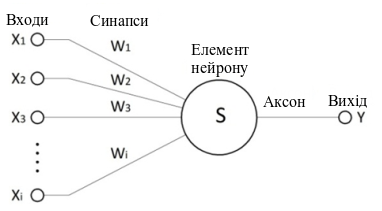
\includegraphics [width=.5\linewidth] {neuron}
	\caption{Загальний вигляд нейрона}
	\label{img:neuron}
\end{figure}

Кожна однонаправлена зв'язок характеризується вагою $w_i$ (величиною синаптичного зв'язку), який за фізичному змісту еквівалентен до електричної провідності. Додатні та відʼємні значення $w_i$ відповідають збудженому або загальмованому стану синапсів. Сума всіх входів визначає поточний стан нейрона \cite{Чураков_2014}

\begin{equation}
\label{eq:equation12}
s=\sum_{i=1}^n x_i w_i.
\end{equation}

Вихід нейрона є функція його стану:

\begin{equation}
\label{eq:equation13}
y=f(s).
\end{equation}

При використанні НМ в задачі розпізнавання мовних сигналах необхідно побудувати відповідну певну для цього завдання мережу, далі навчити її множині мовних сигналів --- підібрати вагові коефіцієнти синапсів для досягнення мінімізації кількості помилок.

\subsection{Аналіз з використанням прихованих марковських моделей}

Одним з найбільш ефективних методів обробки (розпізнавання) мовних сигналів є метод з використанням ПММ. ПММ - статистична модель, що імітує роботу процесу, схожого на марковский процес з невідомими параметрами. Головним завданням СММ є визначення (розгадування) невідомих параметрів на основі спостережуваних. Отримані параметри можуть бути використані в подальшому аналізі, наприклад, для розпізнавання образів.

Застосування ПММ в розпізнаванні грунтується на наступних припущеннях \cite{Огнев_2013}:

\begin{itemize}
	\item мовний сигнал може бути сегментований на фрагменти (стани), всередині яких сигнал може розглядатися як стаціонарний. Перехід між цими станами здійснюється миттєво;
	\item ймовірність появи символу, що породжується моделлю, залежить тільки від поточного стану моделі і не залежить від попередніх породжених символів.
\end{itemize}

Існує кілька типів ПММ, що розрізняються за своєю топологією. Детально топології ПММ розглянуті в \cite{Моттль_1999}.

Для прикладу на рис. \ref{img:hmm} представлена топологія подібної ПММ з трьома станами. ПММ є кінцевий автомат, що змінює свій стан в кожен дискретний момент часу $n$. Перехід зі стану $S_i$ в стан $S_j$ здійснюється випадковим чином з ймовірністю $a_{ij}$. У кожен дискретний момент часу модель породжує вектор спостережень $O_n$ з ймовірністю $b_j(O_n)$.

\begin{figure}
	\centering
	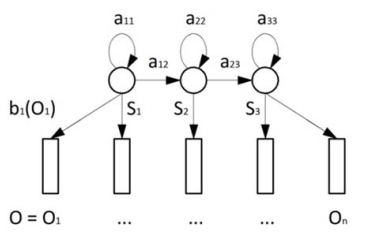
\includegraphics [width=.5\linewidth] {hmm}
	\caption{Топологія ПММ з трьома станами}
	\label{img:hmm}
\end{figure}

\subsection{Аналіз з використанням динамічного трансформування часу}

Відомо, що мовний сигнал швидко змінюється в часі. Різні вимови одного і того ж слова зазвичай мають різну тривалість, а вимови одного і того ж слова однаковою тривалості відрізняються в середині через різні частини слова, які вимовляються з різною швидкістю. Щоб отримати оцінку розбіжності між двома мовними сигналами, представленими як вектори, має бути виконано вирівнювання за часом, який можна реалізувати за допомогою ДТВ \cite{Goldenstein_2013}.

ДТВ є методом еластичного порівняння вектора спостережень з шаблоном, що зберігається. Вектор спостережень і шаблон лежать на відповідних осях сітки (рис. \ref{img:dtt}). Для кожного осередку сітки вираховується різниця між відповідними фрагментами вектора спостережень і шаблону. Оптимальне вирівнювання між вектором спостережень і шаблоном показано маршрутом, що проходить по сітці.

\begin{figure}
	\centering
	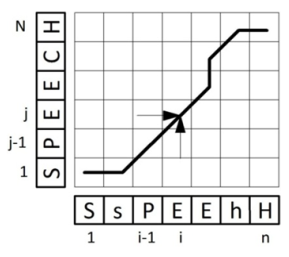
\includegraphics [width=.5\linewidth] {dtt}
	\caption{Робота методу динамічного програмування}
	\label{img:dtt}
\end{figure}

Метод ДТЧ працює з фрагментами, тобто аналіз ознак складається з обробки вектора ознак в регулярних інтервалах. Так як вектор ознак може мати безліч фрагментів, потрібні засоби розрахунку локальної оцінки відстані. Оцінка відстані між двома векторами ознак розраховується за допомогою Евклідової відстані

\begin{equation}
\label{eq:equation14}
d(x,y)=\sqrt{\sum_i(x_i-y_i)^2},
\end{equation}

\noindent
де $x_i$, $y_i$ --- порівнювані фрагменти; $i$ --- номер фрагменту.

Хоча обчислення Евклідової відстані в обчислювальному відношенні не вигідно в порівнянні з будь-якою іншою операцією, воно дає найкращі результати для розпізнавання.

На малюнку шаблон показаний вертикально, а спостережуваний сигнал --- горизонтально. Вхідний сигнал «SsPEEhH» --- це зашумлена версія шаблону «SPEECH». Ідея методу полягає в тому, що «h» --- це найближче збіг з «H» в порівнянні з чимось ще в шаблоні. Вхідний сигнал «SsPEEhH» порівнюється з усіма шаблонами, що зберігаються в словнику. Результатом порівняння буде шаблон, для якого було знайдено мінімальне розходження між вхідним сигналом і шаблоном. Глобальна оцінка розбіжності для маршруту --- це просто сума локальних відстаней між фрагментами сигналу і шаблону \cite{Алимурадов_2015}.

\subsection{Недоліки традиційних систем розпізнання мови}
Сучасні системи розпізнання мови в більшій своїй частині засновані на статистичних методах, використовують потужній апарат теорії ймовірностей та математичної статистики, що дає змогу суттєво підвищити якість розпізнання. Основні методи розпізнання мови --- це приховані Марківські моделі та штучні нейронні мережі \cite{Makovkin_2006, Gefke_2012}. Але у сучасних системах більш поширеними є моделі на нейронних мережах, оскільки вони мають більшу швидкодію та стійкість до шумів \cite{Hinton_2012}.

Звісно, на вхід до нейронної мережі не подають «сирий» звук — амплітуду коливань по часу, адже це не дуже інформативна форма представлення акустичного сигналу для аналізу. Більш інформативним є спектр сигналу, але на практиці найчастіше використовується мел-перетворення, в якому звуковий сигнал нарізується на фрейми розміром 20–40 мс, спектр кожного з яких масштабується через банк фільтрів та логарифмується для отримання даних, найбільш наближених до людського сприйняття \cite{Saini_2013}.

Існує досить багато таких систем і вони доволі якісно виконують свою задачу. Але в більшості своїй ці системи розраховані на роботу в приміщеннях без сильних шумів, залучення дикторів з чіткою вимовою та використання потужних комп’ютерів або віддалених серверів, як, наприклад, Google Voice Search. Та й ці системи неідеальні, в них не вирішені проблеми фільтрації шумів та розпізнання великих об’ємів даних, обмежені можливості налаштування під різні умови та різних дикторів \cite{Volkov_2014}. Так, наприклад, в системах мовного управління бортовим обладнанням літаків мінімальна можлива якість становить 95\%, а час розпізнавання не повинен перевищувати 0,2 с при темпі мовлення порядку 100 слів за хвилину \cite{Bondaros_2007}. Навіть у рамках однієї системи розпізнавання ці параметри можуть змінюватися в залежності від багатьох факторів, у тому числі таких, що визначаються умовами польоту, різними акустичними перешкодами, впливом пілотажних перевантажень тощо. \cite{Korsun_2013}.

Фактично, ті досягнення, які сьогодні здобуті в традиційних системах розпізнання мови, вже можуть бути використані для забезпечення голосової взаємодії в управлінні дистрибуцією. Проте вони не в змозі повністю забезпечити автоматизацію голосової взаємодії в задачах управління дистрибуцією, оскільки немає можливості а ні встановити у кабіні водія потужне обладнання, а ні забезпечити стабільний та швидкісний доступ до інтернету. Крім того, кабіна водія — це неконтрольоване акустичне середовище з високим рівнем шуму. Проблема багатодикторності також актуальна для дистрибуції, адже у таких компаніях зазвичай працює від декількох десятків до кількох сотень і навіть тисяч водіїв, в яких можуть буди дефекти вимови, різноманітні акценти та інші індивідуальні особливості мовлення.

\section{Новітні підходи до автоматизації голосової взаємодії} \label{sect1_5}

Японський дослідник з університету Осаки Ішігуро Хіроші з колегами вивчали різні аспекти комунікації та інформаційно-комунікаційних технологій, як, наприклад, використання комунікації з людиноподібними роботами в якості терапевтичної дії для людей похилого віку \cite{Nishio_2015}, аутистів \cite{Kumazaki_2016} чи просто замкнутих у собі людей, педагогічної дії щодо дітей та немовлят \cite{Park_2015} тощо. Зокрема він проводив дослідження голосової комунікації двох людей опосередковано через комп’ютер \cite{Ishiguro_2016}. 

У цьому дослідженні пара спілкувалася на загальні теми, обираючи варіанти своєї репліки із заздалегідь написаного дерева варіантів, свого роду сценарію. Жодному з партнерів не потрібно було нічого промовляти вголос: людині надавався набір з варіантів реплік на вибір, потрібно було лише натиснути на ту з них, яку б вона хотіла  промовити, і ця репліка лунала з динаміків. У залежності від використаної репліки програма вибирала з дерева сценаріїв можливі варіанти відповідей і надавала їх на вибір співрозмовнику. Співрозмовник у свою чергу, чуючи репліку першої людини, обирав свою з наданих варіантів. Це дослідження було спрямоване на подолання сором’язливості при спілкуванні з особами протилежної статі (що є особливо актуальним для Японії). Але такий підхід заздалегідь написаного дерева сценаріїв комунікації можна використовувати і в інших сферах.

У доповіді на світовому психологічному конгресі 2016 проф. Ішігуро демонстрував використання цього сценарного підходу для роботів на виставках та в музеях. Що б уникнути необхідності розпізнавання голосу в шумному середовищі, поряд з експонатом ставиться людиноподібний робот та монітор, на якому показані варіанти запитань. Натискаючи на різні репліки, відвідувач може спілкуватися з роботом по заздалегідь написаному дереву сценаріїв, розпитуючи його про експонат, а робот буде відповідати голосом.

На жаль для управління дистрибуцією постає зворотне завдання — водій має повідомити певну інформацію в систему і при цьому не повинен відволікатися на натискання кнопок на екрані. Тому пряме використання такої технології неможливе. Але застосування підходу описання всіх можливих сценаріїв комунікації в залежності від контексту дозволить знизити кількість інформації, яку треба розпізнати, а отже і підвищити якість.

Наразi існує новий підхід до голосового управління, заснований на теорії несилової взаємодії \cite{Teslia_2010} — рефлекторна система голосового управління \cite{Egorchenkov_2016}. Ідея, покладена в основу цього підходу, полягає в тому, щоб замість переведення голосової інформації в текстову репрезентацію, аналізувати безпосередньо інформаційну складову сказаного, визначаючи, яку з відомих реакцій потрібно виконати. «Традиційні системи розпізнання мови засновані на принципі: „усна мова“ → „репрезентація мови набором лінгвістичних конструкцій“ → „розуміння мови“. На основі теорії несиловой взаємодій може бути запропонована інша модель розпізнання природної мови: „усна мова“ → „розрахунок несилової (інформаційної) взаємодії на реакції“ → „реакція (розуміння чи поведінка)“» \cite{Teslia_2014}.

Така модель розпізнання називається рефлекторною, оскільки побудована за аналогією зі структурою умовного рефлексу, в якому виділяються афектори, центральний компонент та ефектори. Така модель може бути добре поєднана з ідеєю використання дерева сценаріїв, оскільки сценарії також складаються із реакцій, і одиницею моделювання стає не лінгвістична особливість мовлення, а реакція (або команда), яка може бути врахована автоматизованою системою розраховування маршрутів. Тобто, суть цього підходу полягає в тому, щоб перейти до іншої одиниці розпізнання мови. У психології дискурсивного мислення і рефлексивній психології також накопичено досвід аналізу мови, через виокремлення інших одиниць — функціональних висловлювань \cite{Naydonov_2008}.

Оскільки в такій системі не потрібні словники, складні інтелектуальні моделі аналізу тексту та граматики, вони мають низку переваг порівняно з традиційними системами: багатодикторність, варіабельність природної мови, можливість обробки команд офлайн прямо на пристрої, робота в умовах шумів (неконтрольованого акустично середовища), простота алгоритмів та менша складність і ціна реалізації \cite{Teslia_2013}.

У загальному випадку система рефлекторного голосового управління складається з трьох компонентів:

1. \textit{Фонемний стенограф}

Відповідає за перетворення відцифрованого вхідного звукового сигналу, що поміщає усну мову в набір фонем або слів.

2. \textit{Ядро системи}

Здійснює моделювання системи голосового управління. Містить програмну реалізацію всіх моделей, методів та алгоритмів системи, набір команд, протокол роботи, налаштування тощо.

3. \textit{База даних розпізнання мови з можливістю навчання}

Забезпечує зберігання інформаційної бази розпізнання мови та виділення керуючого впливу. У базі даних зберігається статистика вхідних впливів та відповідних їм вихідних реакцій системи.

Варто зазначити, що модуль фонемного стенографа може бути забезпечений різними програмними засобами, що робить систему гнучкішою та більш адаптивною до умов середовища. Єгорченков \cite{Egorchenkov_2016} наводить перелік можливих модулів фонемного стенографа. Провівши порівняльне зіставлення стенографів з цього переліку, можна стверджувати, що найбільш прийнятним для задач дистрибуції є фонетичний стенограф на основі Julius speech recognition tool \cite{Pylypenko_2009}, оскільки він у своїй роботі не потребує ні доступу до інтернету, ні великих словникових баз, а дає на виході «сирі» фонеми (наприклад, «п ъ й! А м а» для слова «Прямо»), які можуть навіть краще сприйматися рефлекторною системою для подальшого визначення інформаційного компоненту, ніж розпізнані слова, через вищу (в останньому випадку) ймовірність помилки.

\section{Постановка задачі дослідження} \label{sect1_6}

Виходячи з того, що \todo{...}, \textbf{наукова задача} дисертаційної роботи полягатиме в розробці моделей і методів інтеграції формалізації голосової інформації з управлінням процесом дистрибуції в єдиній системі формалізації голосової інформації в системах диспетчерського контролю за рухом автотранспорту.

У процесі вирішення наукової задачі висунута наступна \textbf{гіпотеза}: \todo{...}

\textbf{Основна ідея} даної наукової роботи полягає в тому, що вирішення поставленої наукової задачі можливо за рахунок:

\begin{itemize}
	\item \todo{...}
	\item \todo{...}
\end{itemize}

\textbf{Реалізація} цих ідей в рамках проведених досліджень може бути здійснена на підставі глибокого вивчення, виявлення сильних і слабких сторін методів та інструментів \todo{...}

\textbf{Предметною галузю дослідження} є \todo{...}.

\textbf{Дослідження}, результати яких викладені в подальших розділах цієї роботи, спрямовані:

\begin{itemize}
	\item на визначення методики досліджень і побудови \todo{науково-методологічних} основ автоматизації голосової взаємодії (розділ 2);
	\item на розробку методів формалізації голосової інформації в системах диспетчерського контролю за рухом автотранспорту (розділ 3);
	\item на створення засобів формалізації голосової інформації в системах диспетчерського контролю за рухом автотранспорту(розділ 4).
\end{itemize}

\section*{Висновки до розділу 1}
\addcontentsline{toc}{section}{Висновки до розділу 1}
           % Глава 1
\chapter{Підходи до формалізації голосової взаємодії в системі диспетчеризації} \label{chapt2}

\section{Концепція створення системи автоматизації голосової взаємодії} \label{sect2_1}

У результаті аналізу виявлено два найбільш перспективні напрями, поєднання яких дає змогу запропонувати нове принципове рішення і побудувати рефлекторну модель голосової взаємодії в задачах управління дистрибуцією. В основу моделі покладено логічні сценарії взаємодії на тему управління дистрибуцією, які мають враховувати параметри основних причин невідповідності реальної ситуації запланованому маршруту, наприклад, запізнення або відмови обслуговування на точці доставки тощо. Це дає змогу отримати інформацію для прийняття рішення про повернення вантажу на склад, про відміну чи відкладення обслуговування однієї точки доставки, щоб мати можливість встигнути на іншу, більш важливу, про зміну маршруту для обʼїзду затору або про утворення нового маршруту з резервною машиною тощо.

Звичайно, абсолютно всі причини та параметри не можуть бути враховані заздалегідь, але проробка і врахування основної типології дозволить приймати базові рішення та вдаватися до безпосереднього звʼязку з диспетчером лише у складних випадках, що розвантажить водія та канали комунікації і дасть змогу підвищити загальну ефективність дистрибуції.

Найбільш ефективним шляхом розробки дерева сценаріїв рефлекторної взаємодії є використання вхідних параметрів вже створеної системи автоматизації дистрибуції, у тому числі автоматичної побудови маршрутів \cite{as6}, яка зараз проходить широку експериментальну апробацію. Інтеграція модулю голосової взаємодії з цією системою буде значно спрощена, що сприятиме отриманню кращого економічного ефекту.

Виходячи з наявної логіки побудови маршрутів, вже зараз можна назвати принципові блоки сценаріїв, які потрібно буде розробити. Першим етапом, на якому можуть виникнути проблеми розбіжності плану та факту, є етап завантаження на складі (якщо, наприклад, буде виявлений неврахований «перегруз» або «недогруз» машини, будуть відсутні необхідні товари чи працівники складу не встигнуть їх вчасно відібрати, або навіть виявиться, що машина не здатна вийти на маршрут (наприклад, не заводитися на морозі)).

Другий етап сценаріїв голосової взаємодії визначають проблеми, які можуть виникнути в дорозі до певної точки доставки, як, наприклад, ремонт в дорозі по маршруту руху або зміни в правилах руху на деяких вулицях, які ще не відбиті в алгоритмах прокладення маршруту (нові заборони поворотів чи односторонній рух), проблеми з автомобілем на дорозі, які призводять до зниження швидкості або відмови в подальшому русі по маршруту, або найбільш розповсюджена проблема заторів на дорогах. 

Третій етап сценаріїв голосової взаємодії викликаний можливими невідповідностями між планом та фактом в обслуговуванні на точці доставки. Це можуть бути як проблеми зі сторони клієнта («нікого немає вдома», клієнт не має грошей, клієнт відмовляється від замовлення чи стверджує, що він замовляв щось інше), так і проблеми зі сторони водія (запізнення на точку доставки, тобто не потрапляння в заплановане дозволене часове вікно доступності, пошкодження товару тощо). Найбільш поширеною є ситуація, коли водій проводить в точці доставки більше часу, ніж заплановано, що призводить до проблем на всьому подальшому маршруті.

Ці та інші інциденти на всіх зазначених етапах, що зазначені в моделі на схемі (рис. \ref{img:voice_interaction_schema}), потребують вирішення із залученням диспетчера для вибору найкращої стратегії і мінімізації втрат через проблему. Відповідно дерево сценаріїв голосової взаємодії повинно відбивати всі три етапи та типові відомі проблеми і способи їх розвʼязання.

\begin{figure}
	\centering
	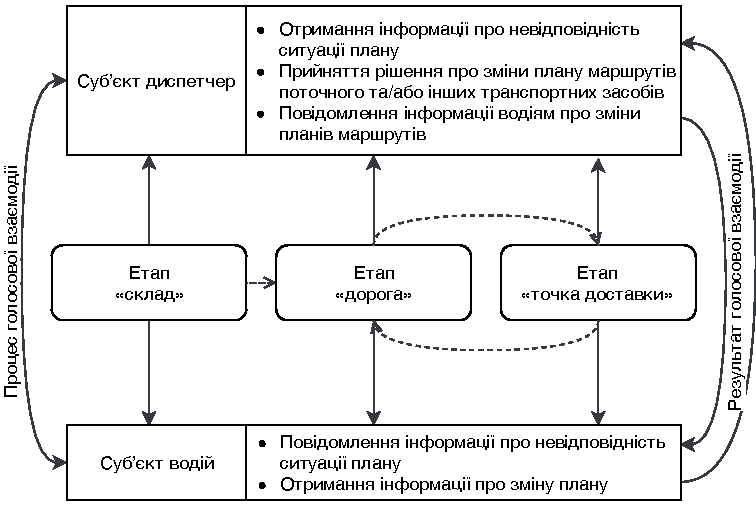
\includegraphics [width=\linewidth] {voice_interaction_schema}
	\caption{Схема голосової взаємодії субʼєктів дистрибуції}
	\label{img:voice_interaction_schema}
\end{figure}

Схема голосової взаємодії субʼєктів дистрибуції зображена на рис. \ref{img:voice_interaction_schema}. Вона складається з трьох етапів, два останніх з яких, можуть циклічно повторюватися при наявності декількох точок доставки в маршруті. Стрілками позначено процеси голосової взаємодії, які можуть розгортатися на кожному з етапів при невідповідності плану та факту. У верхній та нижній частинах схеми показані принципові типи результатів голосової взаємодії для кожного з субʼєктів (диспетчера та водія). Ця логічна схема визначає принциповий алгоритм побудови дерева сценаріїв голосової взаємодії.

Другим важливим та перспективним напрямом, який дає змогу побудувати рефлекторну модель голосової взаємодії в задачах управління дистрибуцією, є застосування рефлекторних систем голосового управління. Ідея, покладена в основу цього підходу, полягає в тому, щоб замість переведення голосової інформації в текстову репрезентацію, аналізувати безпосередньо інформаційну складову сказаного, визначаючи, яку з відомих реакцій потрібно виконати. «Традиційні системи розпізнавання мови засновані на принципі: „усна мова“ → „репрезентація мови набором лінгвістичних конструкцій“ → „розуміння мови“. На основі теорії несиловой взаємодій може бути запропонована інша модель розпізнавання природної мови: „усна мова“ → „розрахунок несилової (інформаційної) взаємодії на реакції“ → „реакція (розуміння чи поведінка)“» \cite{Teslia_2014}.

Тобто така система буде складатися з двох основних компонентів (рис. \ref{img:rgsu_concept}). Перший компонент --- розпізнавання мови, це може бути будь-яка система переведення голосового сигналу в текстову репрезентацію --- як лексичну так і фонетичну. В нашій роботі ми будемо використовувати фонетичну текстову репрезентацію, оскільки її створення не потребує наявності великих контекстно-залежних словників, що більше підходить для використання на мобільному пристрої з обмеженим доступом до мережі інтернет.

\begin{figure}
	\centering
	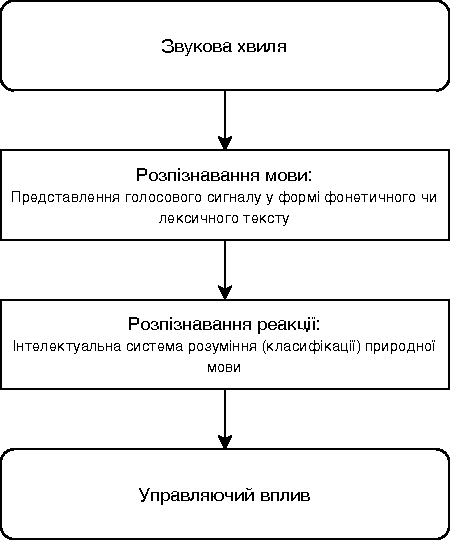
\includegraphics [width=.5\linewidth] {rgsu_concept}
	\caption{Схема узагальненої структури рефлекторних систем голосового управління}
	\label{img:rgsu_concept}
\end{figure}

Другий компонент --- розпізнавання реакції по розпізнаній мові. Концептуально це може бути будь-яка інтелектуальна система розуміння (класифікації) природної мови. В нашій роботі ми будемо розглядати метод інтелектуальних рефлекторних систем, оскільки його ефективність в роботі з фонетичним текстом вже була доведена і метод згорткових нейронних мереж, оскільки вони показали гарні результати при роботі з лексичним текстом посимвольно, що є найбільш схоже на роботу з фонетичним текстом.

\section{Методи автоматизації руху автотранспорту в дистрибуції та параметри що впливають на сценарії голосової взаємодії} \label{sect2_2}

Транспортна логістика --- це система організації доставки, а саме переміщення будь-яких матеріальних предметів або речовин з однієї точки в іншу за оптимальним маршрутом. Транспортна логістика є частиною процесів дистрибуції, курʼєрської доставки, та інших транспортних систем, що включають в себе перевезення вантажів. Важливим етапом в процесах транспортної логістики є так званий етап «останньої милі» --- останній етап доставки вантажу з розподільчого центру до клієнта. Цей етап найменш ефективний з усього ланцюгу поставок, і може коштувати до 28\% від усієї вартості доставки. \cite{Scott_2009}

Для транспортної логістики на етапі останньої милі дуже важливим є планування маршрутів, а також моніторинг та диспетчеризація процесу доставки. Адже якісний маршрут дозволяє зменшити транспортні витрати, а моніторинг --- підвищує рівень сервісу в реакціях на позапланові ситуації. 

На жаль сьогодні в більшості компаній України планування відбувається на достатньо примітивному рівні --- логісти визначають який транспортний засіб повезе який вантаж, але не створюють конкретний маршрут, залишаючи це рішення на водіїв. Це повʼязано в першу чергу з тим що логісти розробляють планові маршрути вручну без залучення автоматизованих систем. Друга причина, що випливає з першої --- логісти не можуть гарантувати принципову виконуваність маршрутів, оскільки орієнтуються в більшій мірі на масо-габаритні параметри, а часові вимоги враховують лише частково. Адже масо-габаритні параметри можна порахувати сумарно незалежно від порядку обʼїзду точок доставки, а часові параметри можливо перевірити лише для конкретного маршруту, побудова і розрахунок якого виходить за межі людських можливостей без використання технічних засобів. Оскільки набір точок доставки для кожного окремого транспортного засобу не є гарантовано виконуваним, то розраховувати маршрути окремих транспортних засобів не має сенсу --- потрібно вирішувати задачу в цілому для всіх точок доставки та машин, що відноситься до суттєво складнішого класу задач --- Vehicle Routing Problem (VRP).

Запровадження автоматичного розрахунку маршрутів несе в собі декілька суттєвих переваг. По перше це гарантованість принципової виконуваності маршрутів, без урахування позапланових ситуацій. По друге це підвищення рівня сервісу, адже маючи конкретний маршрут з плановим часом прибуття, ми можемо повідомити його клієнту, скоротивши його час очікування. Наприклад якщо клієнт замовив доставку з 15:00 до 18:00, він не буде 3 години <<сидіти на стільці>> в очікуванні доставки --- він в цей час лише переважно буде знаходитися в місці доставки, але буде займатися своїми справами, можливо на щось відволічіться чи відійде на короткий час. Якщо ми повідомимо клієнту орієнтовний час доставки (наприклад з 17:00 по 17:30), то ми забезпечимо клієнту більшу свободу дій, та знизимо ймовірність того, що саме в час прибуття доставки, клієнт не зможе її прийняти вчасно, що призведе до затримки.

По третє наявність планового маршруту підвищить можливості моніторингу та реакції на позапланові ситуації. Без планового маршруту, за допомогою GPS моніторингу можливо лише побачити де перебував транспортний засіб та де він зупинявся. Але оскільки невідомий план за яким рухається водій, не зрозуміло, чи зупинка означає обслуговування точки доставки, чи водій відклав цю точку пізніше за планом і просто проїжджав повз, а зупинка --- наприклад, очікування світлофора. Крім того, не маючи плану руху транспортного засобу, не можна спрогнозувати, чи курʼєр встигає обслуговувати усі точки доставки вчасно --- можливо побачити лише факт того що якась із точок не відвідана, а замовлений клієнтом час уже вийшов. Маючи плановий маршрут, можливо в кожний момент часу спрогнозувати приблизний час прибуття на кожну з наступних точок із урахуванням можливого відставання, і побачити чи не призводить це відставання до порушення замовлених клієнтом часових вікон в майбутньому. Маючи цю інформацію набагато легше прийняти своєчасні дії --- повідомити водію про необхідність пришвидшити обслуговування точок або обговорити з клієнтом можливість перенесення часу доставки.

Варто не відкидати також і можливу економію за рахунок покращення ефективності планових маршрутів після запровадження автоматизованого планування. Тим не менше практика показує, що водій, який добре знає ввірену йому територію планує свій маршрут на достатньо високому рівні. Іноді рівень який може забезпечити водій з досвідом роботи навіть кращий за автоматизовані рішення, за рахунок наявності більш детальної інформації про карту району. Тим не менше автоматизоване планування може відвʼязати якість маршрутів від людського фактору --- рівня досвіду кожного конкретного водія.

Точне вирішення задачі маршрутизації транспортних засобів неможлива для розмірів задач, з якими стикаються сучасні курʼєрські служби в містах-мегаполісах. Навіть не всі евристичні алгоритми можуть задовольнити сучасні потреби у швидкості обрахунку. В залежності від бізнес-процесів конкретної компанії та організації системи обліку та контролю за помилками, бувають ситуації коли остаточна інформація про наявні замовлення отримується лише після прибуття вантажу на розподільчий пункт і часу на планування, завантаження та відправлення курʼєрів залишається дуже мало, тому час розрахунку стандартної задачі в 2--3 тисячі точок доставки не може займати більше 30--40 хвилин.

Основна проблема впровадження систем побудови планових маршрутів на практиці полягає у спротиві інноваціям на рівні кінцевих виконавців. Водії, особливо, якщо це наймані перевізники, а не співробітники компанії, відмовляються їхати по запропонованим програмою маршрутам. Перевізників не дуже хвилює глобальна оптимальність всіх маршрутів чи рівень сервісу кінцевого клієнта, якщо до цих параметрів не привʼязана їх платня. Вони звикли отримувати маршрутний лист сформований лише за територіальними та масо-габаритними критеріями, а до часових обмежень кінцевих клієнтів ставитися доволі формально. Тому будь-які зміни звичних планів сприймаються дуже негативно, аж до саботування всього процесу. Навіть в ідеально правильному рішенні може бути необхідність заїхати на територію іншого водія для доставки в деякі точки, які інший водій не встигне виконати або необхідність доставляти точки в районі який водій погано знає, оскільки його знайомому районі в певний день мале навантаження і він може весь бути обслугований сусідами без участі цього водія, а в іншому місці навпаки навантаження велике і потрібно залучення додаткових машин. Але більшість наявних евристик орієнтуються лише на сумарну вартість, і може робити подібного роду помилки в формуванні окремого маршруту, навіть коли в цьому немає нагальної необхідності.

Таким чином постає необхідність розробки евристичного алгоритму який би максимально враховував вимоги логістів та водіїв, щодо оптимальності вибору точок з точки зору кожного конкретного маршруту, при цьому не відкидаючи глобальну оптимальність при високій швидкості обрахунку.

Практика показує, що одним з найбільш визначальних вхідних параметрів, що може сильно вплинути на результат планування та можливість його втілення у  реальність, є кількість часу, що запланована на обслуговування в точок. Адже інші параметри визначені достатньо чітко - масо-габаритні параметри відомі заздалегідь, дозволені часові вікна визначає кінцевий клієнт. Для визначення часу та відстані руху по дорозі між двома точками, є багато вже розроблених інструментів, які прогнозують результат з достатнім рівнем похибки на основі статистичних даних. Але для визначення часу обслуговування точки немає достовірного джерела інформації: ані клієнт, ані водій, ані логіст не можуть його назвати. Найбільш розповсюджена помилка --- писати всім точкам однаковий час, наприклад 10 чи 5  хвилин, незалежно від ваги та кількості вантажу який необхідно доставити або складності пошуку та підʼїзду до точки доставки. Кращий варіант, який можна зустріти доволі часто - категоризація точок або конкретних замовлень, використовувати фіксований час обслуговування для всіх замовлень в категорії. Найбільш правильним варіантом, що може принести суттєву економію транспортного ресурсу при побудові планових маршрутів, є статистичний аналіз історії часу обслуговування точок. Моделювати кількість часу необхідного для виконання точки, потрібно виходячи з наступних параметрів: скільки часу використовувалося на обслуговування цієї та схожих точок в минулому, якими водіями та на яких машинах вони при цьому обслуговувалися, яку вагу, обʼєм та кількість вантажу було доставлено, та інші. Питання вибору оптимального способу моделювання заслуговує окремого дослідження.

Тим не менше, для подібного статистичного аналізу, постає проблема збору цих історичних даних. Достатньо точно час зупинки можна визначити за допомогою аналізу GPS треку, але цей метод має ряд недоліків. По перше, GPS дані мають похибку, яка може збільшуватись як в залежності від якості апаратного забезпечення, так і в залежності від території що обслуговується. Наприклад відомо що зонах висотної забудови GPS сигнал істотно погіршується, а іноді навіть втрачається повністю. Таке погіршення сигналу може згубно впливати на визначення часу зупинки або навіть факту зупинки взагалі. По друге, навіть якщо відкинути похибку GPS як не суттєву або прийнятну, постає питання співвідношення зупинок та точок доставки. У загальному випадку таке співвідношення однозначно можливе тільки якщо в заданому радіусі є лише одна зупинка та одна точка доставки. У випадках коли зупинка відбулася поза заданим радіусом, коли біля точки було кілька зупинок (в тому числі з причин хибної інтерпретації зупинки через похибки GPS), або, як це трапляється найчастіше, одна зупинка знаходиться близько до декількох точок, --- однозначно співвіднести з якої з зупинок необхідно записати час обслуговування точки неможливо. В сучасному світі, в містах мегаполісах, ситуація коли необхідно зробити декілька доставок в один багатоквартирний будинок, або сусідні будинки зі спільним двором, відбувається достатньо часто, і це автоматично унеможливлює збір та аналіз великої частини статистичної інформації про час обслуговування точки на основі GPS даних.

Отже необхідно доповнити дані GPS додатковою інформацією про те, коли водій-експедитор закінчив виконання однієї з точок в межах єдиної зупинки і почав виконання наступної точки. Практика показує що спроби зобовʼязати водія в цей момент діставати телефон/планшет і вибирати відповідну команду в мобільному додатку експедитора, у кращому випадку призводить лише до того, що водій відмітить всі точки як виконані ще до або вже після виконання всіх доставок на зупинці, адже маніпуляції з планшетом потребують часу, а руки в цей момент зазвичай зайняті. Для вирішення цієї проблеми потрібен зручний для водія/експедитора інтерфейс, який би не відволікав його від основного завдання. Таким може виступати голосовий інтерфейс, який буде сприймати команди про початок та завершення виконання доставки.


\section{Методи представлення дерева сценаріїв взаємодії з урахуванням не голосової інформації} \label{sect2_3}

Для представлення дерева сценаріїв найкраще підходить орієнтований граф, в якому вершини позначають стан системи та діалогові фрази які буде озвучувати система, а ребра --- репліки (стимулів) які можуть бути сприйняті системою в кожній конкретній вершині. Реакція на стимул може привести до переходу між станами, отже орієнтоване ребро проводиться від тієї вершини в якій стимул може бути сприйнятий, до тієї, в який стан система перейде в якості реакції на стимул. Отже множина всіх ребер, що виходять з вершини, позначають перелік стимулів, між якими треба проводити розпізнання для стану, що відповідає цей вершині.

Назва «дерево» сценаріїв використовується як сталий вираз, але реально представити всю необхідну інформацію у вигляді дерева неможливо, адже переходи між станами неминуче приводять до утворення циклів, а отже граф для представлення такої інформації підходить краще.

На жаль такій схемі недостатньо повноти для представлення всіх можливих варіантів перебігу подій. По перше реакції системи не обмежуються переключенням станів (контекстів) що позначають доступний перелік стимулів та відтворенням діалогових фраз. Основне корисне навантаження системи --- комунікація між водієм і диспетчером та керування процесом доставки, а отже нам необхідний спосіб представлення інших реакцій на стимули, таких як відправлення певної інформації в диспетчерський центр, отримання інструкцій з диспетчерського центру, переключення внутрішніх змінних для можливості повідомити водію контекстно-залежну інформацію про "поточну" точку доставки, тощо.

По друге стимули які можуть викликати певні реакції системи і відповідно переходи між станами не обмежуються голосовими репліками сказаними водієм. Це можуть бути певні події які надійшли з інших джерел інформації, наприклад, команда від диспетчера на зміну маршруту, відміну чи перенос точки доставки, або інформація з внутрішніх джерел даних --- датчиків GPS, роботи двигуна чи відкриття дверей. Використовуючи інформацію з внутрішніх датчиків, можливо автоматизувати перехід між деякими станами, що підвищить зручність користування системою да ще зменшить кількість необхідних альтернатив для розпізнавання голосових стимулів. 

Отже для повноцінного опису ми маємо такі сутності:

\begin{itemize}
	\item \textbf{Контекст} або \textbf{Стан}, що задає перелік дозволених стимулів, які може сприйняти система в знаходячись в цьому контексті
	\item \textbf{Стимул} або \textbf{Подія} --- певна зовнішня інформація що породжує відповідну реакцію. Стимул може бути голосовою реплікою від водія, командою отриманою від диспетчера або подією породженою інформацією з внутрішніх датчиків, якщо вони доступні
	\item \textbf{Реакція} системи відповідно до стимулу. Рекцією може бути переключення контексту, відтворення діалогового голосового повідомлення, відправлення певної моніторингової інформації до диспетчерського центру,  переключення внутрішніх змінних, тощо. Один стимул може породжувати декілька реакцій різних типів.
\end{itemize}


\section{Принципи побудови рефлекторної системи голосової взаємодії водія в системах диспетчерського контролю за рухом автотранспорту} \label{sect2_4}

\subsection{Застосування теорії несилової взаємодії як основи інтелектуальних рефлекторних систем} \label{subsect2_4_1}

Принципи побудови рефлекторних систем лежать у теорії несилової взаємодії. У роботі \cite{Teslia_2010} представлена компʼютерна модель ймовірнісної інтерпретації руху, згідно з якої єдина швидкість з якою переміщуються обʼєкти --- швидкість світла у вакуумі, а очікувана швидкість дрейфу для будь-якого матеріально обʼєкта $V$ залежить лише від імовірності його зсуву в тому чи іншому напрямі і дорівнює:

\[
V=c\cdot(p-(1-p))=c\cdot(2p-1)
\]

\noindent
де $p$ --- ймовірність зсуву у напрямку руху; $c$ --- швидкість світла у вакуумі

Згідно з зазначеною теорією кожен обʼєкт в межах компʼютерної моделі має певну власну визначеність щодо руху в одному чи іншому напрямку. 

\[
p=\frac{i^+}{i^+ + i^-}
\]

\noindent
де $i^+$ --- розмір області визначення напрямку зміщення обʼєкта у напрямку руху; $i^-$ --- розмір області визначення напрямку зміщення обʼєкта проти напрямку руху.

Автор вводить величини визначеності та інформованості:

\begin{equation}
\label{eq:tnv3}
d=i^+ - i^-;
\end{equation}

\begin{equation}
\label{eq:tnv4}
i=i^+ + i^-,
\end{equation}

\noindent
де $d$ --- визначеність щодо зміщення у напрямку руху; $i$ --- інформованість щодо зміщення у напрямку руху.

Крім того компʼютерної моделі автор доводить що для руху матеріальних обʼєктів ці величини взаємозалежні і можуть бути обраховані з формули: 

\begin{equation}
\label{eq:tnv7}
i=\sqrt{d^2+1}.
\end{equation}

З приведених вище формул можна вивести наступні залежності \cite{Teslia_2010}:

\begin{equation}
\label{eq:tnv5}
p=0.5+\frac{d}{2i};
\end{equation}

\begin{equation}
\label{eq:tnv6}
V=\frac{dc}{i};
\end{equation}

\begin{equation}
\label{eq:tnv8}
d=\pm0.5\sqrt{\frac{p}{1-p}+\frac{1-p}{p}-2}.
\end{equation}

Якщо застосувати фізичні закони до інформаційно-ймовірнісної інтерпретації руху, отриманої з компʼютерної моделі, що лежить в основі теорії несилового взаємодії, то можна отримати вирази для оперування визначеністю \cite{Teslia_2010_2}. З формули релятивістського додавання швидкостей отримано вираз для операції доповнення визначеності:

\begin{equation}
\label{eq:tnv9}
d_{xy}=d_yi_x-d_xi_y.
\end{equation}

Якщо відома визначеність та додаткова визначеність, то можна визначити нову визначеність:

\begin{equation}
\label{eq:tnv10}
d_y=d_xi_{xy}+d_{xy}i_x.
\end{equation}

З інформаційної інтерпретації закону збереження імпульсу отримано вираз для складання визначеності

\begin{equation}
\label{eq:tnv11}
d_\Sigma = \sum_{j=1}^N d_j.
\end{equation}


\subsection{Використання рефлекторного методу для побудови рефлекторної системи голосової взаємодії} \label{subsect2_4_2}

Принцип побудови рефлекторних систем будується на гіпотезі, що не тільки рух матеріальних обʼєктів у розробленій компʼютерній моделі, а й усі системи різного рівня складності підкоряються цим законам. Так, наприклад, автор показує що зазначені формули теорії несилової взаємодії відповідають статистичним закономірностям у природно-мовному тексті \cite[розділ 8]{Teslia_2010}.

Для побудови інтелектуальних рефлекторних систем припускається залежність сумісної умовної ймовірності реакції від безумовної ймовірності реакції та часткових умовних ймовірностей реакції в цій системі підкоряється фізичним законам збереження імпульсу компʼютерної моделі, і можуть бути розраховані по приведеним вище формулам.

Алгоритмічної основою таких систем є рефлекторний метод обчислення адекватної реакції на сукупність різних слабоструктурованих вхідних впливів.

Якщо застосувати принципи теорії несилової взаємодії до рефлекторних систем голосової взаємодії водія та диспетчера, то під реакцією буде розумітися та чи інша команда з моделі голосової взаємодії, а під умовним впливом буде розумітися наявність того чи іншого набору N-грам фонем.

Схема реалізації цього методу включає етапи:

1. Розрахунок визначеності для інтелектуальної системи відносно всіх вхідних N-грам фонем і можливих голосових команд.

Аналогія визначеності реакцій і впливів у фізичній компʼютерні моделі --- це імпульс матеріальних обʼєктів. У такій моделі розглядаються дві групи обʼєктів --- що впливають шляхом «зіткнення» та передачі власної інформації (імпульсу) обʼєктам, на які здійснюється вплив (відповідно можливим реакціям, голосовим командам). З (\ref{eq:tnv7}) та (\ref{eq:tnv8}) отримуємо:

\[
d(A_i)=\pm0.5\sqrt{\frac{p(A_i)}{1-p(A_i)}+\frac{1-p(A_i)}{p(A_i)}-2};
\]

\[
i(A_i)=\sqrt{d^2(A_i)+1};
\]

\[
d(A_i/B_j)=\pm0.5\sqrt{\frac{p(A_i/B_j)}{1-p(A_i/B_j)}+\frac{1-p(A_i/B_j)}{p(A_i/B_j)}-2};
\]

\[
i(A_i/B_j)=\sqrt{d^2(A_i/B_j)+1},
\]

\noindent
де: $p(A_i)$ --- безумовна ймовірність вибору команди $A_i$; $d(A_i)$ --- визначеність щодо команди $A_i$; $i(A_i)$ --- інформованість щодо команди $A_i$; $p(A_i/B_j)$ --- умовна ймовірність вибору команди $A_i$ (при наявності N-граму фонем $B_j$); $d(A_i/B_j)$ --- визначеність щодо команди $A_i$ при наявності N-граму фонем $B_j$; $i(A_i/B_j)$ --- інформованість щодо команди $A_i$ при наявності N-граму фонем $B_j$.

2. З інформаційно-ймовірнісної інтерпретації формули релятивістського додавання швидкостей (\ref{eq:tnv9}) отримано додаткову визначеність, що є у N-грамів фонем відносно голосових команд. Аналогією цього у фізичній компʼютерній моделі є швидкість руху впливаючих обʼєктів відносно обʼєктів, на які здійснюється вплив:

\[
\Delta d(A_i/B_j)=d(A_i/B_j)\cdot i(A_i)-d(A_i)\cdot i(A_i/B_j)
\]

\noindent
де $\Delta d(A_i/B_j)$ --- додаткова визначеність щодо команди $A_i$ яку надає наявність N-граму фонем $B_j$.

3. З інформаційно-ймовірнісної інтерпретації закону збереження імпульсу у компʼютерній моделі (\ref{eq:tnv11}) розраховано сумарний вплив на голосову команду, реакцію інтелектуальної системи. Аналог «удару» безлічі рухомих обʼєктів (відповідних дій) в обʼєкти, відповідні реакцій

\[
d_\Sigma(A_i) = \sum_j \Delta d(A_i/B_j); \\
\]

\[
i_\Sigma(A_i) = \sqrt{\Delta d^2(A_i/B_j)+1},
\]

\noindent
де $d_\Sigma(A_i)$ --- сумарна додаткова визначеність щодо команди $A_i$ під впливом всіх N-грамів фонем $B_j$; $i_\Sigma(A_i)$ --- сумарна доповнювальна інформованість щодо команди $A_i$ під впливом всіх N-грамів фонем $B_j$.

4. Обчислюється нова визначеність голосової команди. Аналогом у фізичній компʼютерній моделі є нова швидкість руху після отриманого імпульсу під час зіткнення з обʼєктами, що впливають)

\begin{equation}
\label{eq:ifron2}
d(A_i/B)=d_\Sigma(A_i)\cdot i(A_i)+d(A_i)\cdot i_\Sigma(A_i),
\end{equation}


\[
i(A_i/B) = \sqrt{d^2(A_i/B)+1},
\]

\noindent
де $d(A_i/B)$ --- нова визначеність щодо команди $A_i$ з урахуванням впливу всіх N-грамів фонем $B_j \in B$; $i(A_i/B)$ --- нова інформованість щодо команди $A_i$ з урахуванням впливу всіх N-грамів фонем $B_j \in B$.

5. За необхідності з (\ref{eq:tnv5}) можна обчислити сумісну умовну ймовірність команди $A_i$ (при наявності всіх N-грамів фонем $B_j \in B$)

\[
p(A_i/B)=0.5+\frac{d(A_i/B)}{2i(A_i/B)};
\]

\noindent
де $p(A_i/B)$ --- сумісна умовна ймовірність команди $A_i$ (при наявності всіх N-грамів фонем $B_j \in B$).

\section*{Висновки до розділу 2}
\addcontentsline{toc}{section}{Висновки до розділу 2}

%У розділі проведено дослідження науково-методологічних основ автоматизації голосової взаємодії. При цьому можна зробити наступні висновки.

1. Запропоновано концепцію створення системи автоматизації голосової взаємодії в задачах управління дистрибуцією, що має дві складові: (а) інтелектуальні рефлекторні системи голосового управління, що включають блок розпізнавання звукового сигналу та блок виділення його змісту; (б) модель сценаріїв взаємодії у процесах дистрибуції на трьох етапах доставки (завантаження на складі, дорога до точки доставки, розвантаження у точці доставки).

% Найбільш перспективним напрямом, який дає змогу запропонувати нове принципове рішення і побудувати рефлекторну модель голосової взаємодії в задачах управління дистрибуцією є застосування моделей логічних сценаріїв взаємодії у процесах дистрибуції, які мають враховувати параметри основних причин невідповідності реальної ситуації запланованому маршруту. При отриманні такої інформації можна буде прийняти рішення про повернення вантажу на склад, про відміну чи відкладення обслуговування однієї точки доставки, щоб мати можливість встигнути на іншу, більш важливу, про зміну маршруту для обʼїзду затору або про утворення нового маршруту з резервною машиною тощо.

% Тому запропоновано модель на трьох етапах дистрибуції, проблемні моменти в якій вирішуються із залученням диспетчера для вибору найкращої стратегії і мінімізації втрат. Структурна модель є принциповим алгоритмом побудови дерева сценаріїв голосової взаємодії для кожного з субʼєктів (диспетчера та водія).

2. Розроблена система автоматичного розрахунку планових маршрутів та практика її використання забезпечили накопичення параметрів непередбачуваних ситуацій на плановому маршруті доставки, що впливають на створення сценаріїв голосової взаємодії.

%Дослідивши методи автоматизації руху автотранспорту в дистрибуції та параметри, що впливають на сценарії голосової взаємодії встановлено, що є необхідність у розробці евристичного алгоритму, який би максимально враховував вимоги логістів та водіїв, щодо оптимальності вибору точок з точки зору кожного конкретного маршруту, забезпечуючи глобальну оптимальність при високій швидкості обчислення.

%Тому запропоновано доповнити дані GPS додатковою інформацією про закінчення виконання однієї з точок в межах єдиної зупинки і початок виконання наступної точки. Для забезпечення зазначеного необхідно впровадити зручний інтерфейс, який не буде відволікати водія від основного завдання, тобто це може бути голосовий інтерфейс, який сприйматиме команди про початок та завершення виконання доставки.

3. Модель голосової взаємодії запропоновано будувати у вигляді орієнтованого графу, в якому вершини позначають стан системи та діалогові фрази, які буде озвучувати система, а ребра – репліки (стимули), які можуть бути сприйняті системою в кожній конкретній вершині, а множина всіх ребер, що виходять з однієї вершини буде позначати перелік стимулів розпізнання для її стану. У результаті для повноцінного опису запропоновано використовувати такі сутності: Контекст або Стан, Стимул або Подія, Реакція системи відповідно до стимулу.

4. Принципи побудови рефлекторних систем на основі теорії несилової взаємодії адаптовано для автоматизації голосової взаємодії в системах диспетчерського контролю за рухом автотранспорту.

%Під час дослідження принципів побудови рефлекторної системи голосової взаємодії встановлено закономірності застосування теорії несилової взаємодії як основи інтелектуальних рефлекторних систем, а також теоретично запропоновано використання рефлекторного методу для побудови рефлекторної системи голосової взаємодії в системах диспетчерського контролю за рухом автотранспорту.
           % Глава 2
\chapter{Методи формалізації голосової інформації в системах диспетчерського контролю за рухом автотранспорту} \label{chapt3}

\section{Класифікація реакцій в системах диспетчерського контролю за рухом автотранспорту} \label{sect3_1}

Для створення класифікації реакцій в системах диспетчерського контролю за рухом автотранспорту було зібрано статистичні дані (зауваження та коментарі) щодо процесу доставки різних вантажів автомобільним транспортом у провідних логістичних компаніях. Систематизація та обробка зібраних оригінальних коментарів до статусу доставки, що використовуються в різних компаніях (табл. \ref{tbl:original_comments}), дали змогу створити відповідну до представленої на рис. \ref{img:voice_interaction_schema} моделі класифікацію голосових команд для субʼєктів дистрибуції «склад – дорога – точка доставки», яку подано нижче.

Для «складу» наявні такі головні коментарі:
\begin{itemize}
	\item проблеми з вантажем:
	\begin{itemize}
		\item відсутня частина товару на складі;
		\item забруднена продукція (пил, бруд, стійкий сторонній запах);
		\item частина товару пошкоджена;
		\item відсутня накладна;
		\item неправильно розраховано тоннаж та/або обʼєм продукції (товар не вміщується в авто);
	\end{itemize}
	\item проблеми з машиною:
	\begin{itemize}
		\item несправність ТЗ;
		\item машина не заводиться;
	\end{itemize}
	\item проблеми з виїздом:
	\begin{itemize}
		\item запізнення прибуття на склад;
		\item затримка завантаження товару на складі при вчасній подачі автомобіля;
	\end{itemize}
	\item інші команди:
	\begin{itemize}
		\item набрати диспетчера;
		\item показати маршрутний лист;
		\item показати мапу маршруту;
		\item виїзд зі складу.
	\end{itemize}
\end{itemize}

Для «дороги» наявні такі головні коментарі:
\begin{itemize}
	\item неможливо досягти точки:
	\begin{itemize}
		\item заблокований вʼїзд/виїзд автомобіля доставки;
		\item немає підʼїзду до будинку (будівельні, дорожні роботи, припаркований транспорт тощо), обʼїхати неможливо;
		\item неправильна адреса або недостатньо інформації для доставки замовлення;
		\item не знайшли адресу;
		\item не було місця для парковки;
		\item авто не змогло під`їхати через габарити;
	\end{itemize}
	\item складнощі з досягненням точки:
	\begin{itemize}
		\item неправильне присвоєння сектору/координат;
		\item похибка при складанні маршруту (адреса точки доставки випадає з логіки загального маршруту);
		\item підʼїзд до будинку з іншої вулиці;
	\end{itemize}
	\item затримки в русі, відхилення від маршруту, можливо, необхідний перерахунок маршруту:
	\begin{itemize}
		\item транспортний затор на маршруті;
		\item будівельні, дорожні роботи, перекриті дороги;
		\item помилка карти - маршрут прокладено по неіснуючій дорозі;
	\end{itemize}
	\item неможливо продовжувати маршрут:
	\begin{itemize}
		\item транспортний засіб потрапив у ДТП;
		\item поломка ТЗ на маршруті;
		\item складні погодні умови (автотранспорт фізично не може доїхати до місця доставки);
	\end{itemize}
	\item інші команди:
	\begin{itemize}
		\item набрати диспетчера;
		\item набрати клієнта;
		\item показати маршрутний лист;
		\item показати мапу маршруту;
		\item показати інформацію про точку;
		\item прибув у точку.
	\end{itemize}
\end{itemize}

Для «точки доставки» наявні такі головні коментарі:
\begin{itemize}
	\item відсутність клієнта:
	\begin{itemize}
		\item клієнт забув про доставку;
		\item особисті причини (клієнт не зміг бути вчасно);
		\item клієнта немає на місці, звʼязок з ним відсутній (некоректний номер телефону для звʼязку, недодзвін);
		\item невчасне (запізнення/випередження) прибуття на точку доставки, клієнт не має змоги прийняти товар;
	\end{itemize}
	\item немає можливості виконати доставку:
	\begin{itemize}
		\item не працює ліфт, клієнт проживає вище Х поверху;
		\item закрито доступ до приміщення клієнта;
		\item у клієнта відсутні необхідні документи, матеріали чи товар для відвантаження;
	\end{itemize}
	\item відмова клієнта прийняти товар:
	\begin{itemize}
		\item відмова на місці;
		\item немає грошей;
		\item пошкоджений або відсутній товар:
		\begin{itemize}
			\item товар не завантажено;
			\item товар забруднений;
			\item товар недоукомплектовано;
			\item товар не працює (внутрішня поломка);
			\item товар пошкоджено зовні;
		\end{itemize}
	\end{itemize}
	\item помилка в замовленні:
	\begin{itemize}
		\item не робили замовлення взагалі;
		\item замовляли на інший день;
		\item замовляли на іншу адресу;
		\item замовляли на інший час;
		\item замовляли інший товар;
	\end{itemize}
	\item часткове виконання замовлення:
	\begin{itemize}
		\item задвоєне замовлення, половина товару повертається;
		\item у документах зазначено товар, який клієнт не замовляв;
	\end{itemize}
	\item інші команди:
	\begin{itemize}
		\item набрати диспетчера;
		\item набрати клієнта;
		\item показати маршрутний лист;
		\item показати мапу маршруту;
		\item показати інформацію про точку;
		\item почав виконання наступної точки;
		\item точка успішно виконана.
	\end{itemize}
\end{itemize}

\section{Модель голосової взаємодії водія в системах диспетчерського контролю за рухом автотранспорту} \label{sect3_2}

\subsection{Побудова орієнтованого графу сценаріїв голосової взаємодії}

Як зазначалося в попередньому розділі, дерево сценаріїв може бути застосоване для голосової взаємодії субʼєктів дистрибуції «склад – дорога – точка доставки» відповідно до моделі, що наведена на рис. \ref{img:voice_interaction_schema}. Найпростіше дерево сценаріїв для моделі голосової взаємодії водія в системах диспетчерського контролю за рухом автотранспорту можна представити в такий спосіб (рис. \ref{img:01_simplest_positive_scenario}).

\begin{figure}
	\centering
	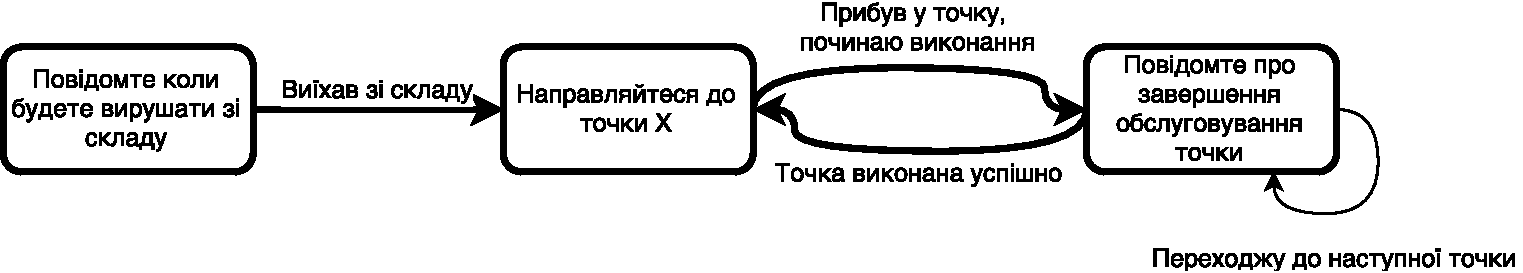
\includegraphics [width=1\linewidth] {01_simplest_positive_scenario}
	\caption{Найпростіше дерево сценаріїв}
	\label{img:01_simplest_positive_scenario}
\end{figure}

Таке саме найпростіше дерево сценаріїв для моделі голосової взаємодії водія в системах диспетчерського контролю за рухом автотранспорту тільки з вертикальним розподілом наведено на рис. \ref{img:02_simplest_positive_scenario_vertical}.

\begin{figure}
	\centering
	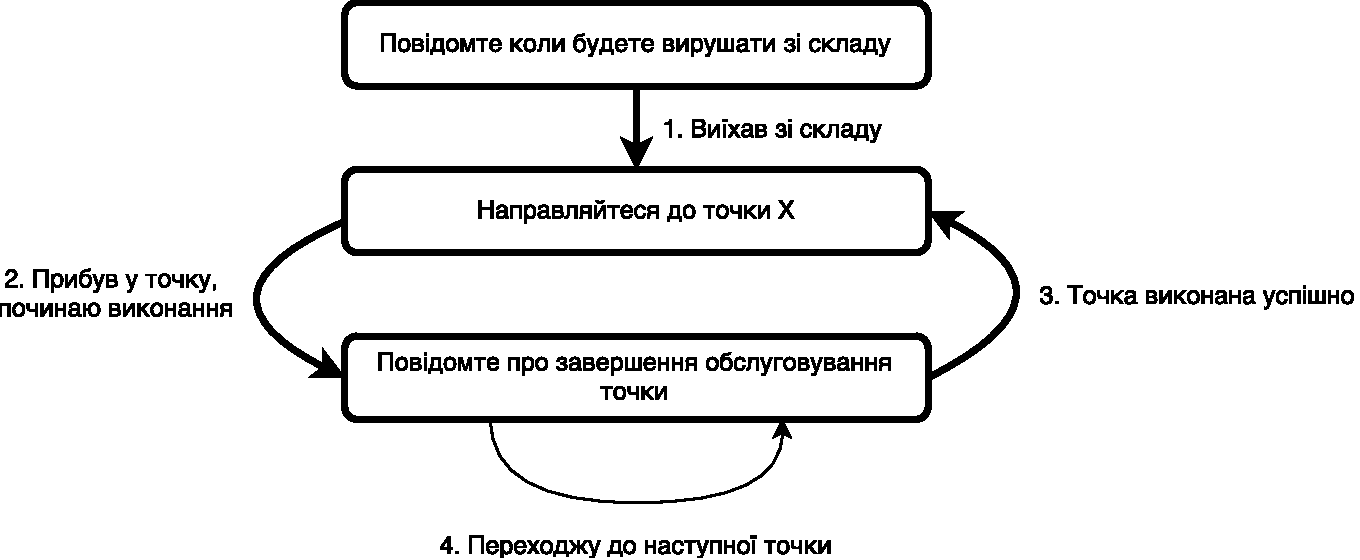
\includegraphics [width=1\linewidth] {02_simplest_positive_scenario_vertical}
	\caption{Вертикальний розподіл найпростішого дерева сценаріїв}
	\label{img:02_simplest_positive_scenario_vertical}
\end{figure}

Найпростіше дерево сценаріїв (рис. \ref{img:01_simplest_positive_scenario}, \ref{img:02_simplest_positive_scenario_vertical}) показує всі доступні варіанти (послідовність подій) в моделі голосової взаємодії водія в системах диспетчерського контролю за рухом автотранспорту. Кожна така послідовність (або ланцюжок) подій повинна представлятися окремим сценарієм.

Для випадку позитивного підтвердження обслуговування або виконання відповідної точки в моделі голосової взаємодії водія в системах диспетчерського контролю за рухом автотранспорту побудовано позитивне дерево сценаріїв (рис. \ref{img:03_positive_scenario_with_conformation}).

\begin{figure}
	\centering
	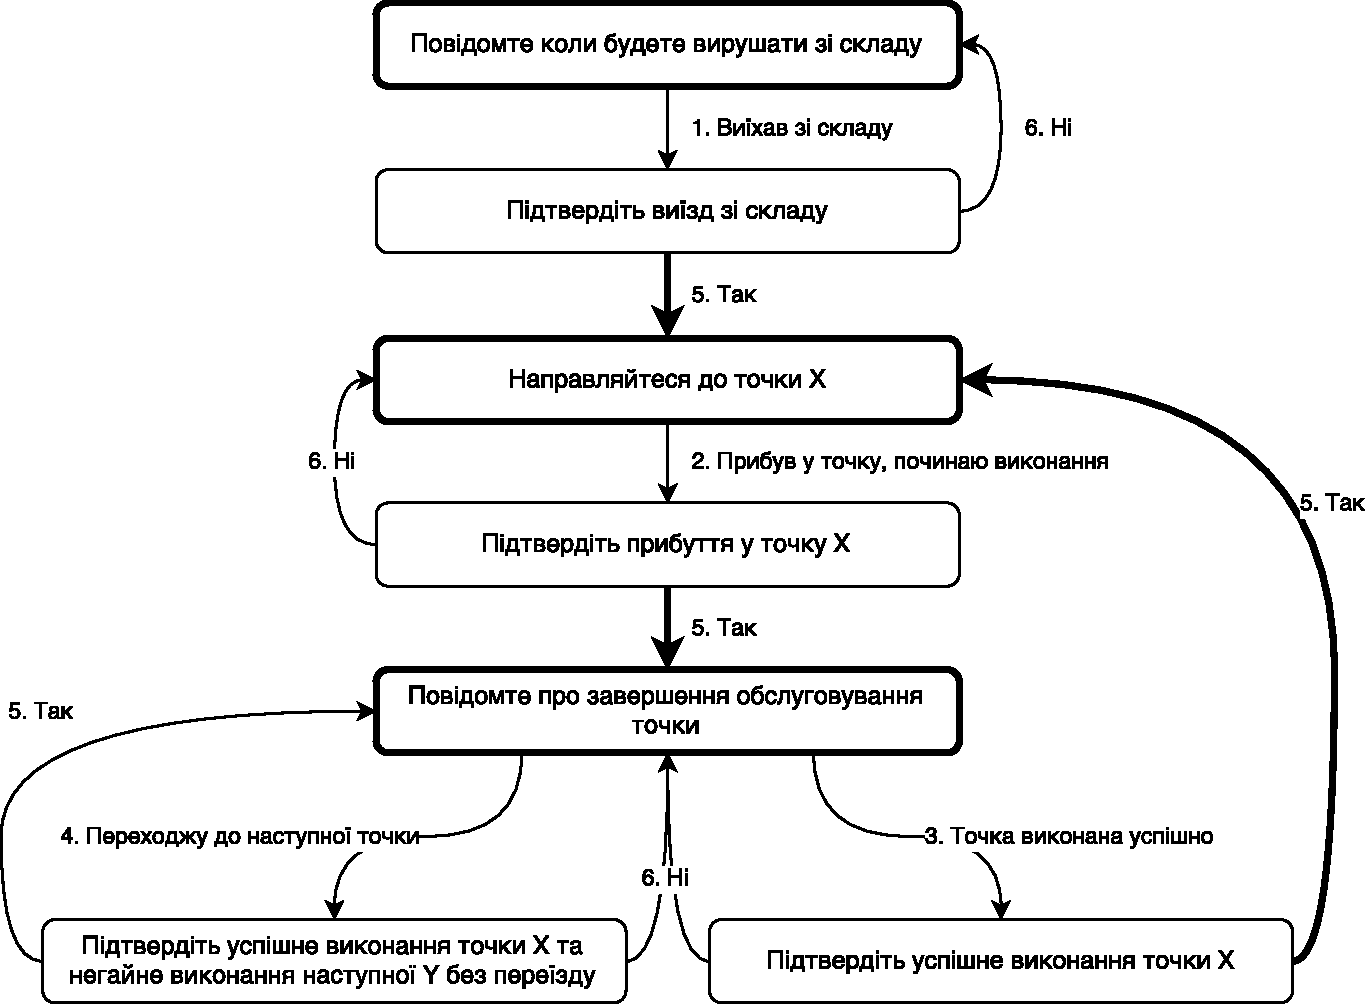
\includegraphics [width=1\linewidth] {03_positive_scenario_with_conformation}
	\caption{Позитивне дерево сценаріїв з підтвердженням}
	\label{img:03_positive_scenario_with_conformation}
\end{figure}

Наведене позитивне дерево сценаріїв з підтвердженням обслуговування або виконання відповідної точки (рис. \ref{img:03_positive_scenario_with_conformation}) є більш складним порівняно з найпростішим деревом сценаріїв (рис. \ref{img:01_simplest_positive_scenario}, \ref{img:02_simplest_positive_scenario_vertical}).  Це ключова відмінність цього дерева від попереднього, де враховано можливість відміни команди, помилково розпізнаної системою, або помилкової команди водія. Позитивне дерево сценаріїв є достатнім для ідеального світу, де все відбувається за планом. Як бачимо, для даного випадку обслуговування або виконання відповідної точки відбувається без позапланових ситуацій на відміну від дерева сценаріїв з негативними інцидентами, перший варіант якого наведено на рис. \ref{img:04_first_negative_scenario_with_conformation}.

На рис. \ref{img:04_first_negative_scenario_with_conformation} зʼявляється додатковий блок, повʼязаний з підтвердженням того, що точку Х не вдалося виконати, тобто дерево сценаріїв враховує можливі негативні інциденти в моделі голосової взаємодії водія в системах диспетчерського контролю за рухом автотранспорту.

\begin{figure}
	\centering
	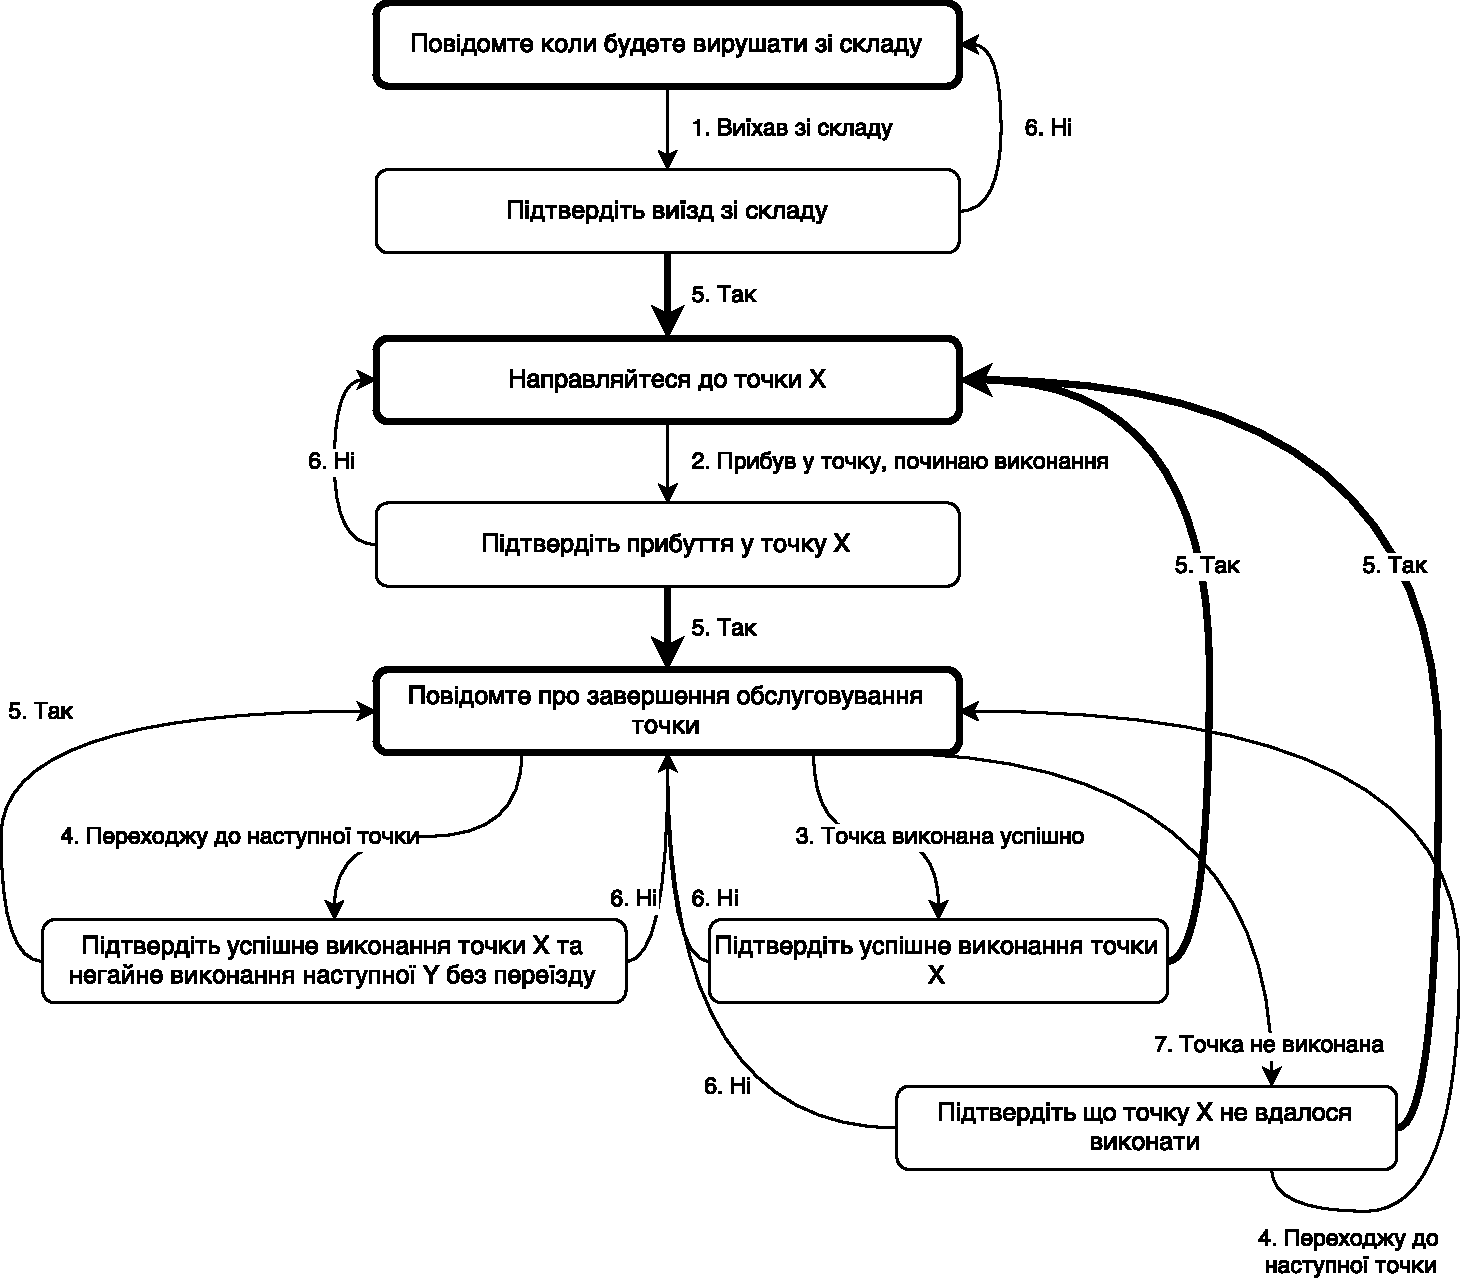
\includegraphics [width=1\linewidth] {04_first_negative_scenario_with_conformation}
	\caption{Перший варіант дерева сценаріїв з негативними інцидентами}
	\label{img:04_first_negative_scenario_with_conformation}
\end{figure}

Спрощений варіант дерева сценаріїв у моделі голосової взаємодії водія в системах диспетчерського контролю за рухом автотранспорту з негативними інцидентами наведено на рис. \ref{img:05_simple_negative_scenario_with_conformation}. У цьому варіанті блок з підтвердженням успішного виконання точки Х, з негайним виконанням наступної точки Y без переїзду трансформується в блок, повʼязаний з підтвердженням того, що точку Х не вдалося виконати, і стає, по суті, спрощеним варіантом дерева сценаріїв з негативними інцидентами, що наведений на рис. \ref{img:04_first_negative_scenario_with_conformation}.

\begin{figure}
	\centering
	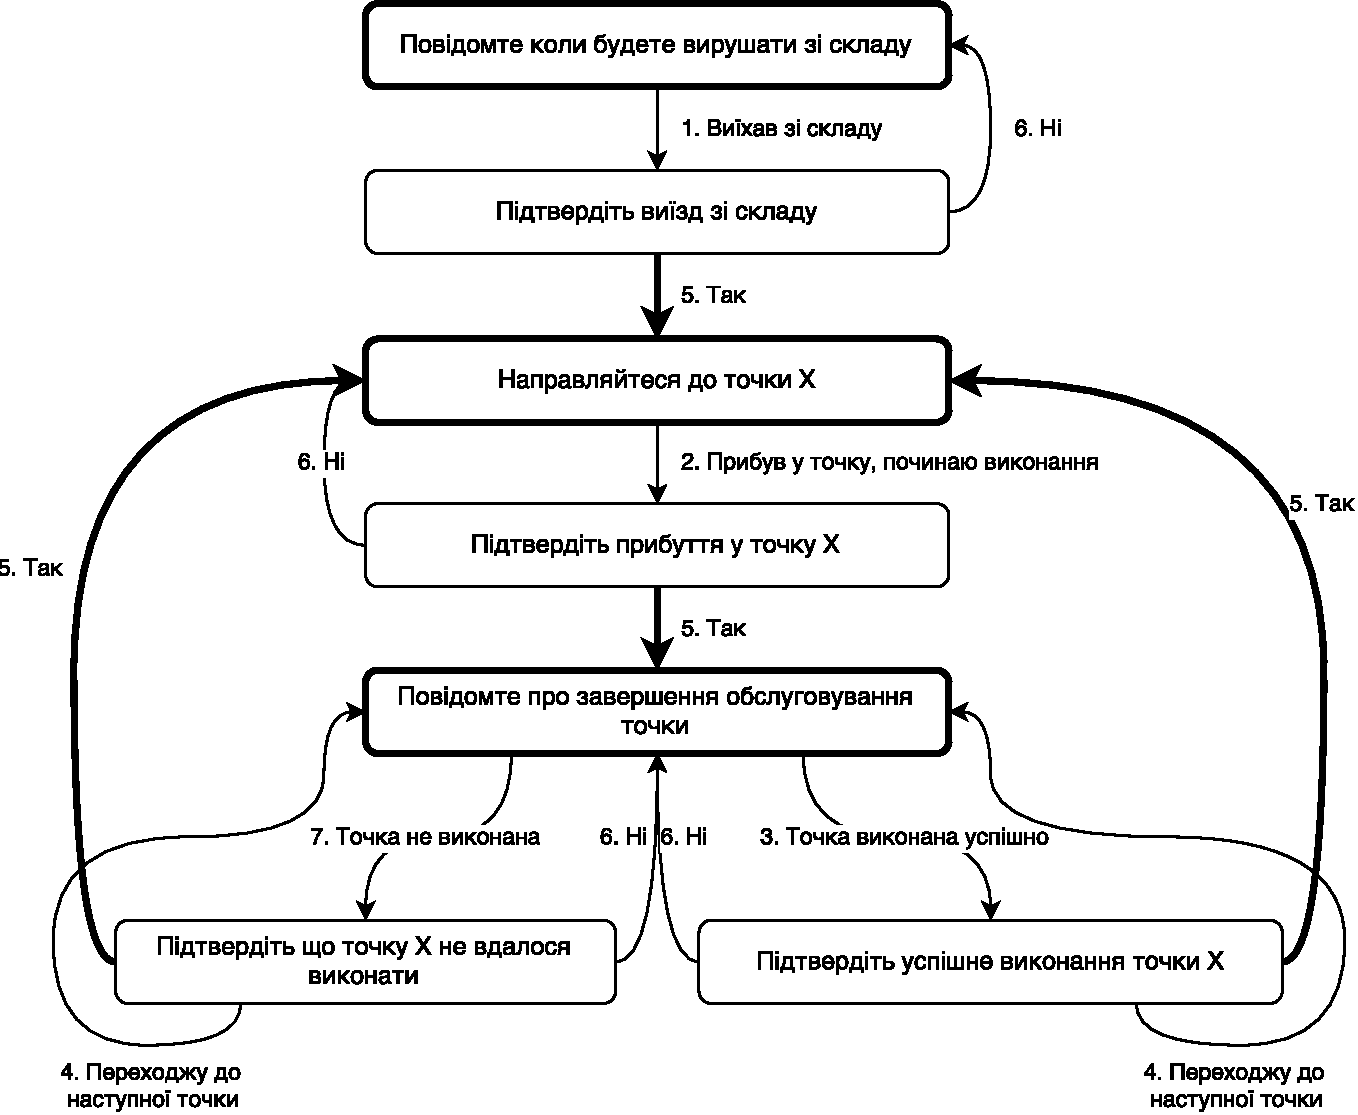
\includegraphics [width=1\linewidth] {05_simple_negative_scenario_with_conformation}
	\caption{Спрощений варіант дерева сценаріїв з негативними інцидентами}
	\label{img:05_simple_negative_scenario_with_conformation}
\end{figure}

Також у моделі голосової взаємодії водія в системах диспетчерського контролю за рухом автотранспорту може бути запропонований один з варіантів дерева сценаріїв з негативними інцидентами та відміною виконання ("відбоєм") (рис. \ref{img:06_simple_negative_scenario_with_rollback}). Для наведеного випадку в дереві сценаріїв зʼявляється блок, повʼязаний з підтвердженням неприбуття в точку Х. Тобто, в дереві сценаріїв зʼявляється звʼязок з відміною виконання та обслуговування точки Х при моделюванні голосової взаємодії водія в системах диспетчерського контролю за рухом автотранспорту. У "спрощеному" варіанті прибирається додаткове підтвердження для "переходжу до наступної точки". Щоб зберегти стійкість до помилок і простоту діалогу, замість підтвердження додаємо можливість відмінити цю останню дію.

\begin{figure}
	\centering
	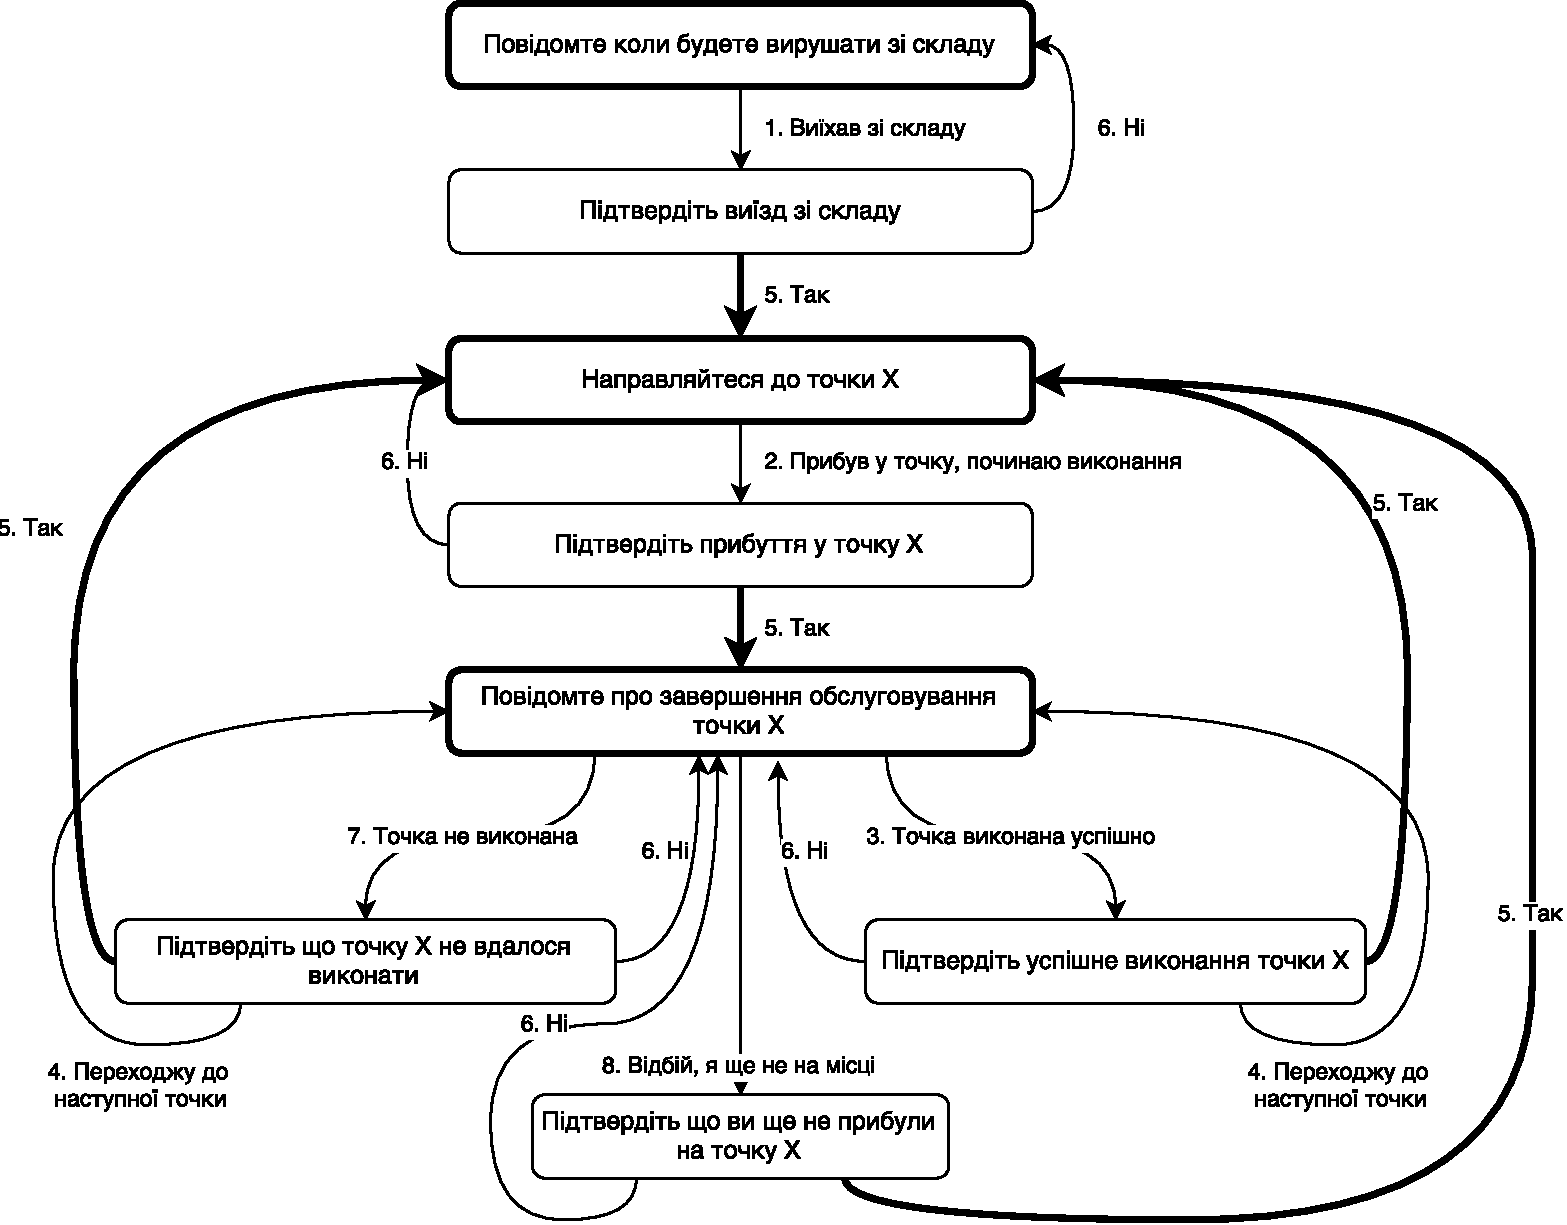
\includegraphics [width=1\linewidth] {06_simple_negative_scenario_with_rollback}
	\caption{Варіант дерева сценаріїв з негативними інцидентами та відбоєм}
	\label{img:06_simple_negative_scenario_with_rollback}
\end{figure}

Оскільки дерево стає занадто великим для зображення, для подальшої деталізації розібʼємо його на частини відповідно до трьох основних етапів. Частину дерева сценаріїв етапу «точка доставки» у вертикальному розподілі наведено на рис. \ref{img:07_simple_point_scenario}, у горизонтальному – на рис. \ref{img:07_simple_point_scenario_horizontal}.
Наведені фрагменти дерева сценаріїв етапу «точка доставки» у вертикальному (рис. \ref{img:07_simple_point_scenario}) та горизонтальному (рис. \ref{img:07_simple_point_scenario_horizontal}) розподілах містять виконання та обслуговування попередньої точки Y, поточної точки Х та наступної точки Z, що розташовані на відповідних дорогах.

\begin{figure}
	\centering
	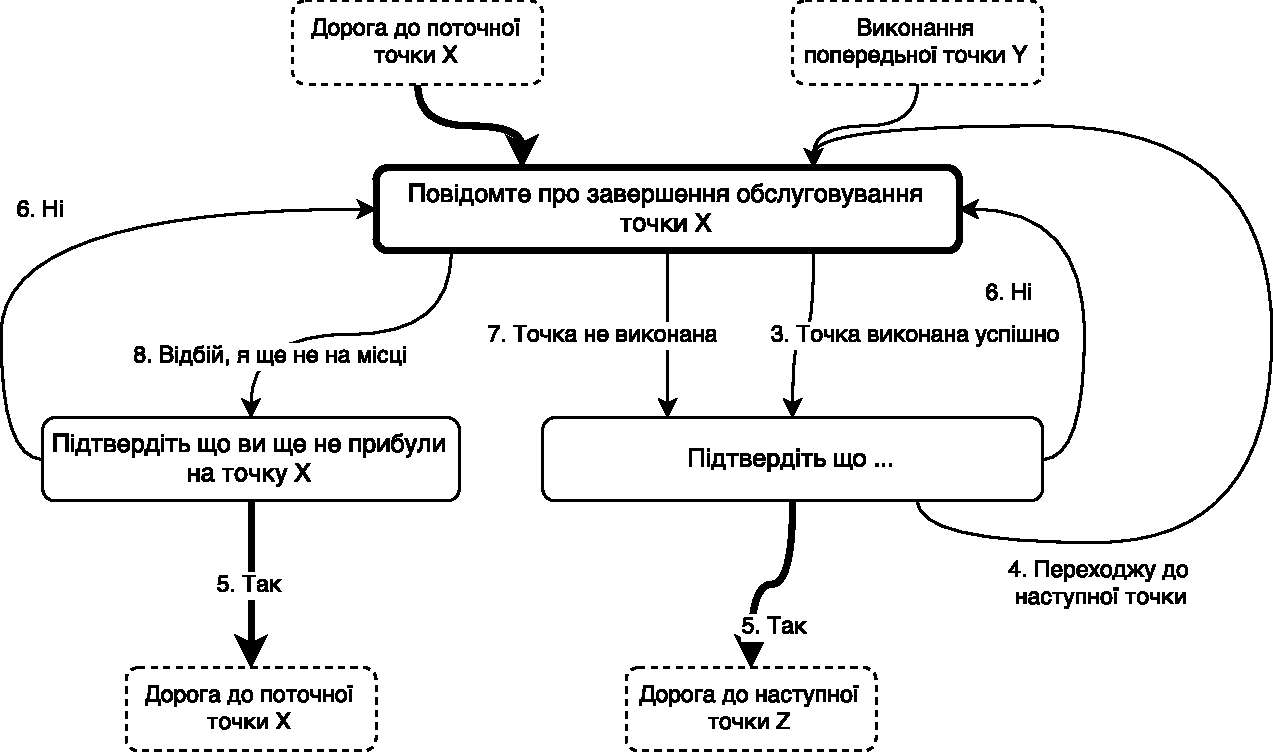
\includegraphics [width=1\linewidth] {07_simple_point_scenario}
	\caption{Частина дерева сценаріїв етапу <<точка доставки>>}
	\label{img:07_simple_point_scenario}
\end{figure}

\begin{figure}
	\centering
	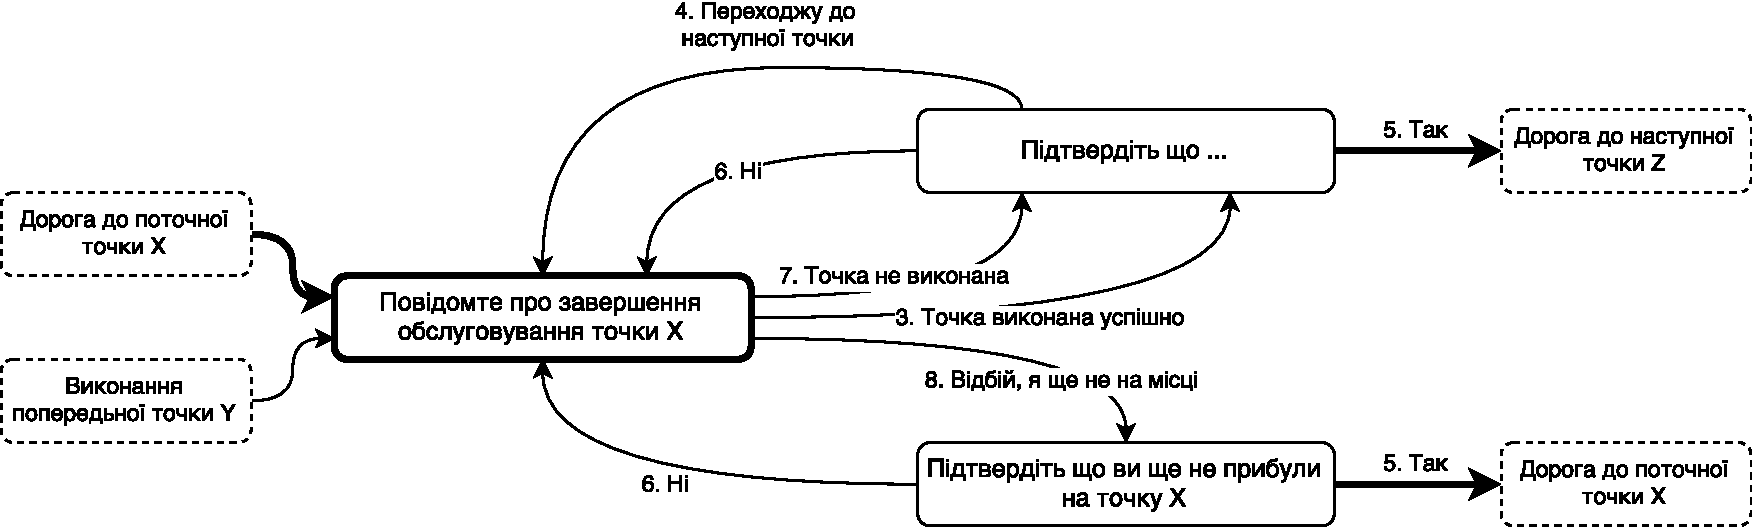
\includegraphics [width=1\linewidth] {07_simple_point_scenario_horizontal}
	\caption{Частина дерева сценаріїв етапу <<точка доставки>> в горизонтальному розподілі}
	\label{img:07_simple_point_scenario_horizontal}
\end{figure}

Як бачимо з рис. \ref{img:07_simple_point_scenario} та \ref{img:07_simple_point_scenario_horizontal}, горизонтальний розподіл є більш компактним.
На рис. \ref{img:08_complete_point_scenario} наведено одну з частин дерева сценаріїв етапу «точка доставки» з усіма негативними інцидентами при моделюванні голосової взаємодії водія в системах диспетчерського контролю за рухом автотранспорту.


\begin{figure}
	\centering
	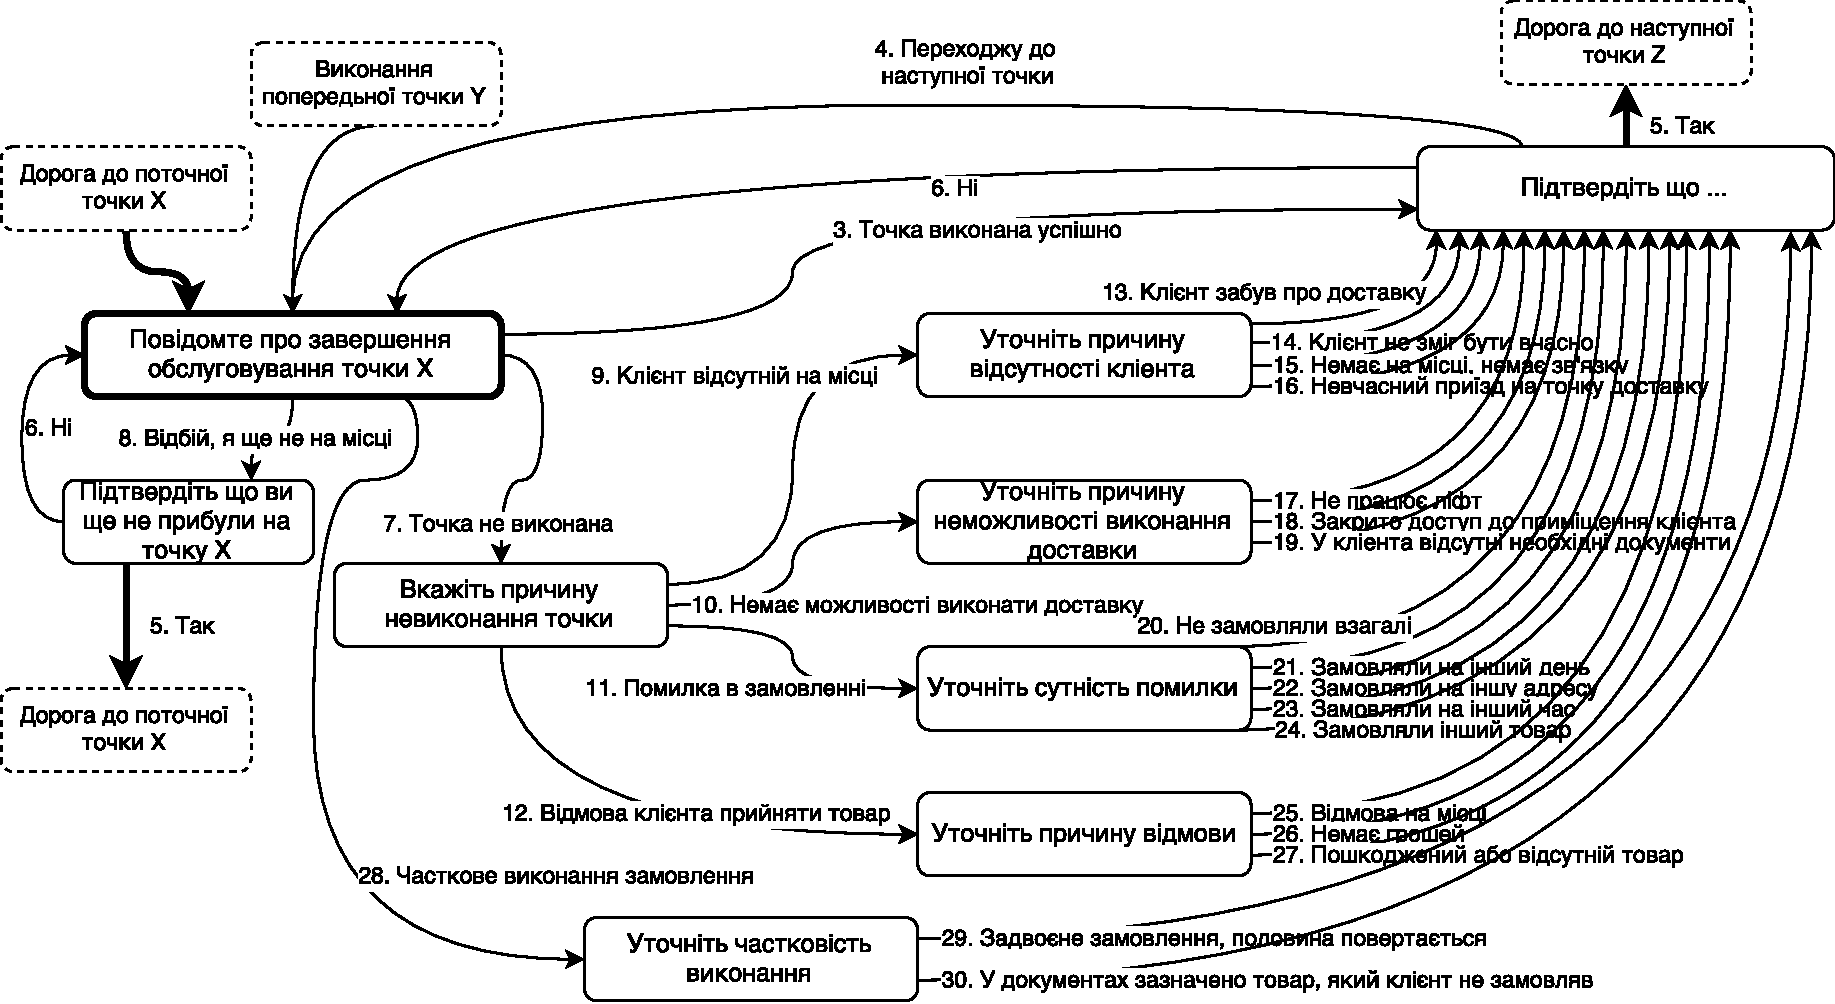
\includegraphics [width=1\linewidth] {08_complete_point_scenario}
	\caption{Частина дерева сценаріїв етапу <<точка доставки>> з усіма негативними інцидентами}
	\label{img:08_complete_point_scenario}
\end{figure}

Наведена частина дерева сценаріїв етапу «точка доставки» (рис. \ref{img:08_complete_point_scenario}) містить блок невиконання точки Х з розширеним уточненням причин та блок часткового виконання з характеристиками такого виконання.

На рис. \ref{img:08_complete_point_scenario_with_other} представлено частину дерева сценаріїв етапу «точка доставки» з усіма негативними інцидентами та врахуванням деяких інших непередбачених подій невиконання точки Х з більш розширеним уточненням причин порівняно з деревом сценаріїв, що представлено на рис. \ref{img:08_complete_point_scenario}, та частковим виконанням з більш розширеними характеристиками такого часткового виконання. Для зберігання відкритості досліджуваної системи на етапі моделювання не можуть бути враховані всі можливі варіанти розвитку подій, тому на рис. \ref{img:08_complete_point_scenario_with_other} наведено деякі непередбачувані події невиконання точки Х.

\begin{figure}
	\centering
	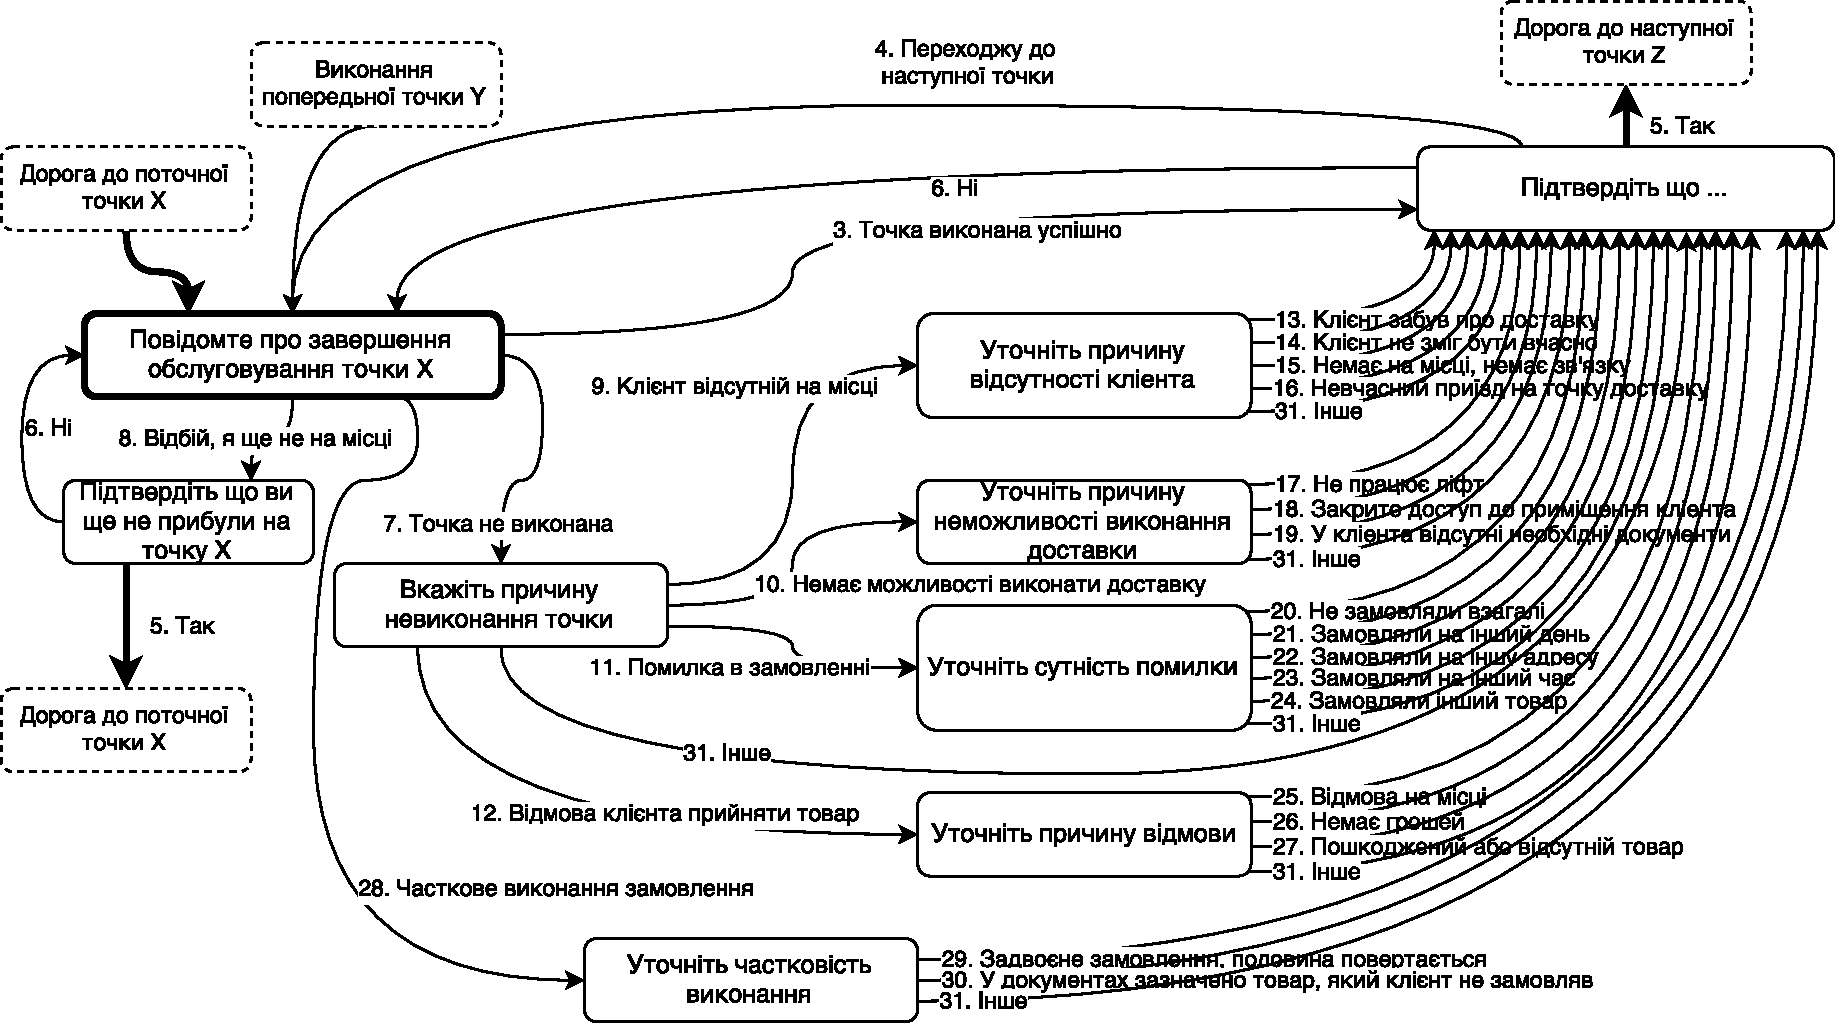
\includegraphics [width=1\linewidth] {08_complete_point_scenario_with_other}
	\caption{Частина дерева сценаріїв етапу <<точка доставки>> з усіма негативними інцидентами та урахуванням інших непередбачених подій}
	\label{img:08_complete_point_scenario_with_other}
\end{figure}

На рис. \ref{img:09_complete_point_scenario_with_rollback} представлено частину дерева сценаріїв етапу «точка доставки» з усіма негативними інцидентами та відбоєм із діалогового режиму. Можемо бачити, що для випадку відбою причин невиконання точки Х із діалогового режиму відбувається перехід до констатації обслуговування та успішного виконання точки Х при моделюванні голосової взаємодії водія в системах диспетчерського контролю за рухом автотранспорту.

\begin{figure} 
	\centering
	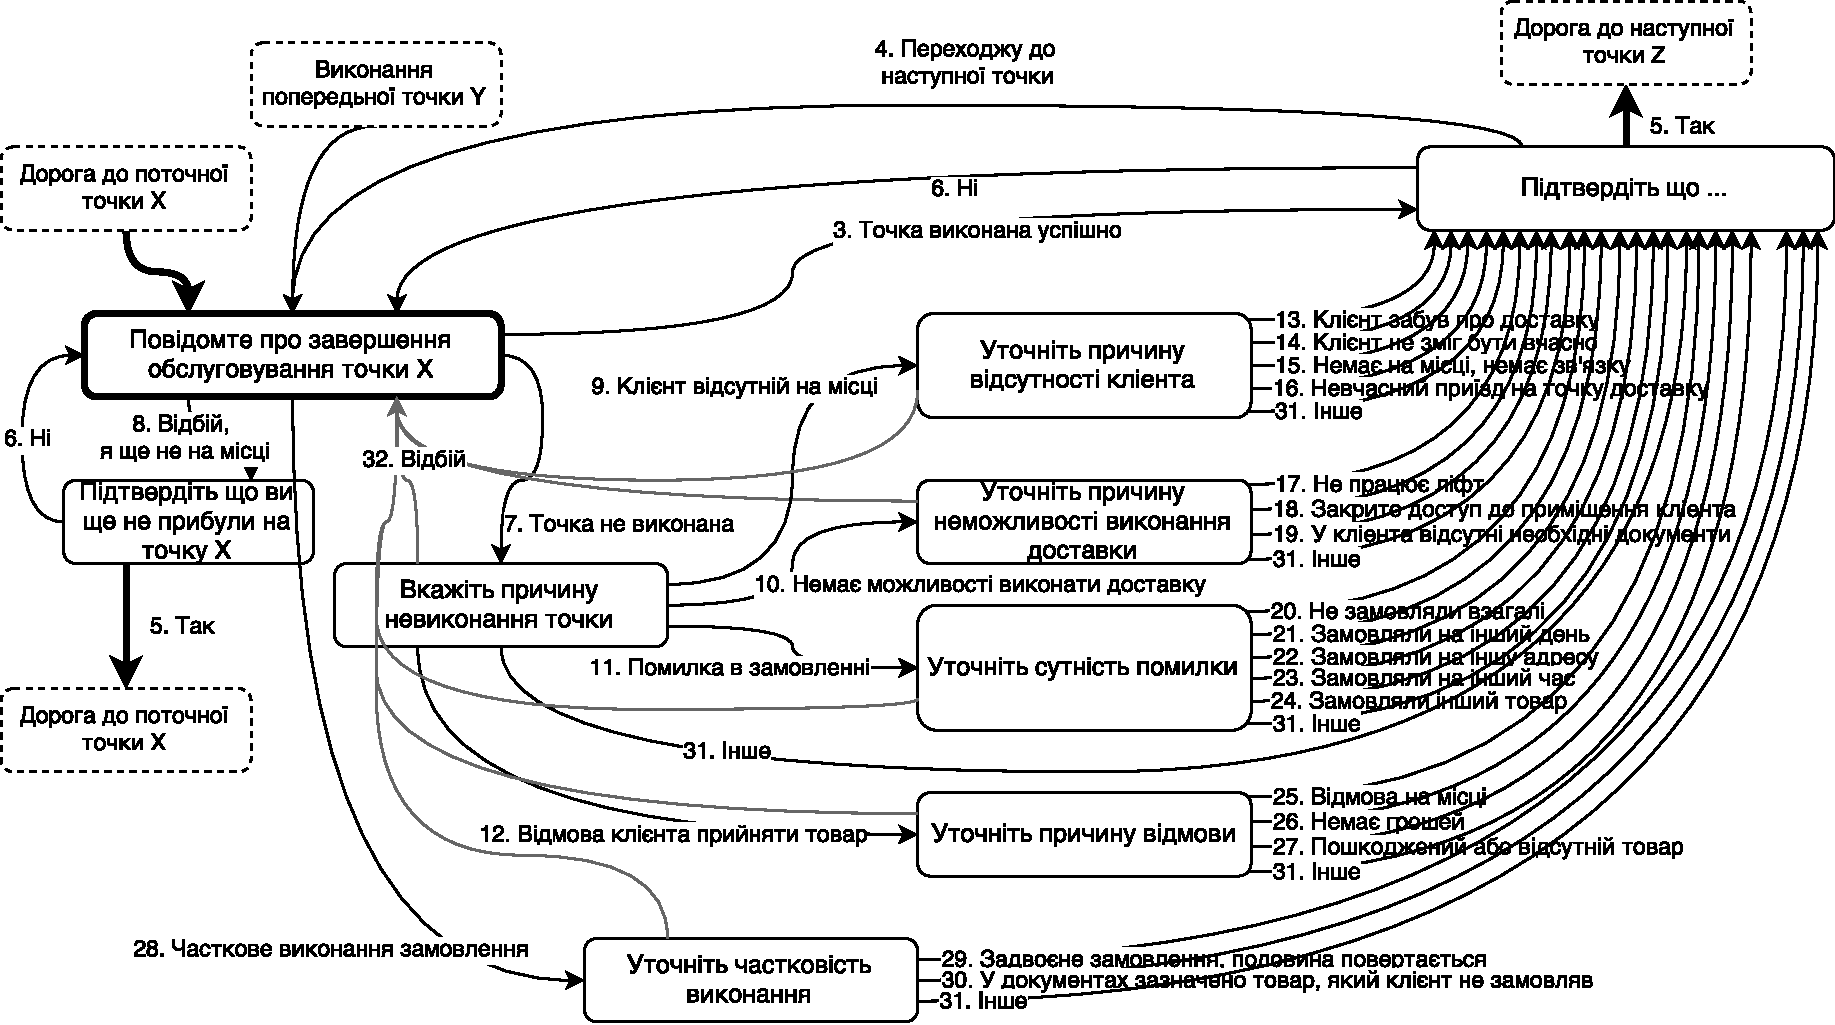
\includegraphics [width=1\linewidth] {09_complete_point_scenario_with_rollback}
	\caption{Частина дерева сценаріїв етапу "точка доставки" з усіма негативними інцидентами та відбоєм із діалогового режиму}
	\label{img:09_complete_point_scenario_with_rollback}
\end{figure}

Для випадку застосування додаткових функцій при моделюванні голосової взаємодії водія в системах диспетчерського контролю за рухом автотранспорту побудовано дерево сценаріїв етапу «точка доставки», частину якого наведено на рис. \ref{img:10_point_scenario_with_enchantment}.

\begin{figure}
	\centering
	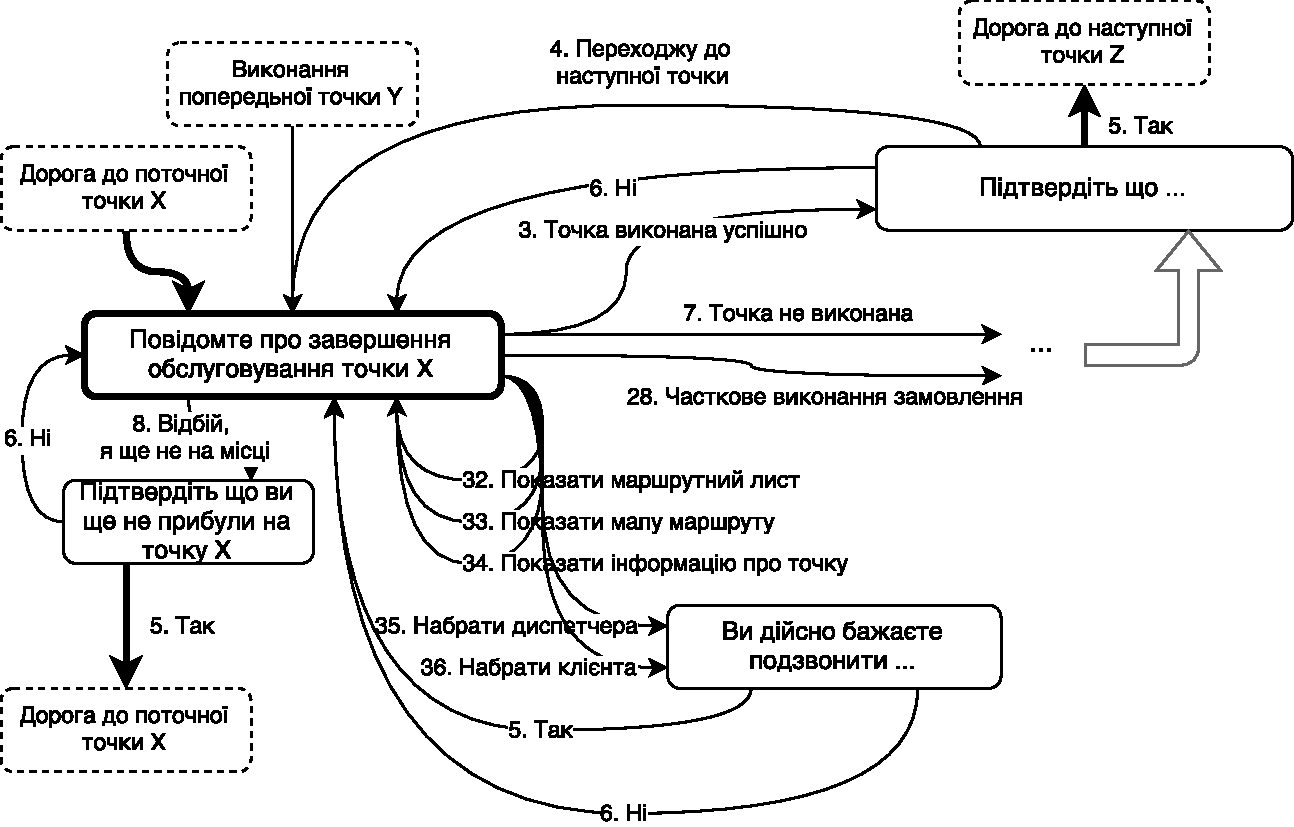
\includegraphics [width=1\linewidth] {10_point_scenario_with_enchantment}
	\caption{Частина дерева сценаріїв етапу <<точка доставки>> з додатковими функціями}
	\label{img:10_point_scenario_with_enchantment}
\end{figure}

У наведеній частині дерева сценаріїв етапу «точка доставки» (рис. \ref{img:10_point_scenario_with_enchantment}) присутні додаткові функції для водія при моделюванні його голосової взаємодії, повʼязані з інформаційними характеристиками маршруту до точки доставки Х, а також функції для набору диспетчера або клієнта.

На етапі «дорога» дерево сценаріїв для моделі голосової взаємодії водія в системах диспетчерського контролю за рухом автотранспорту має наступний вигляд (рис. \ref{img:11_complete_road_scenario}). У наведеній частині дерева сценаріїв етапу «дорога» враховано всі контексти з репрезентативної вибірки даних, які отримано у провідних логістичних компаніях України. При цьому, у випадку невиконання етапу «дорога» пропонуються причини затримки чи неможливості виконання маршруту з наступними інструкціями диспетчера, а у випадку, коли зʼявляється можливість виконання маршруту до точки доставки Х, існує відбій із діалогового режиму.

\begin{figure}
	\centering
	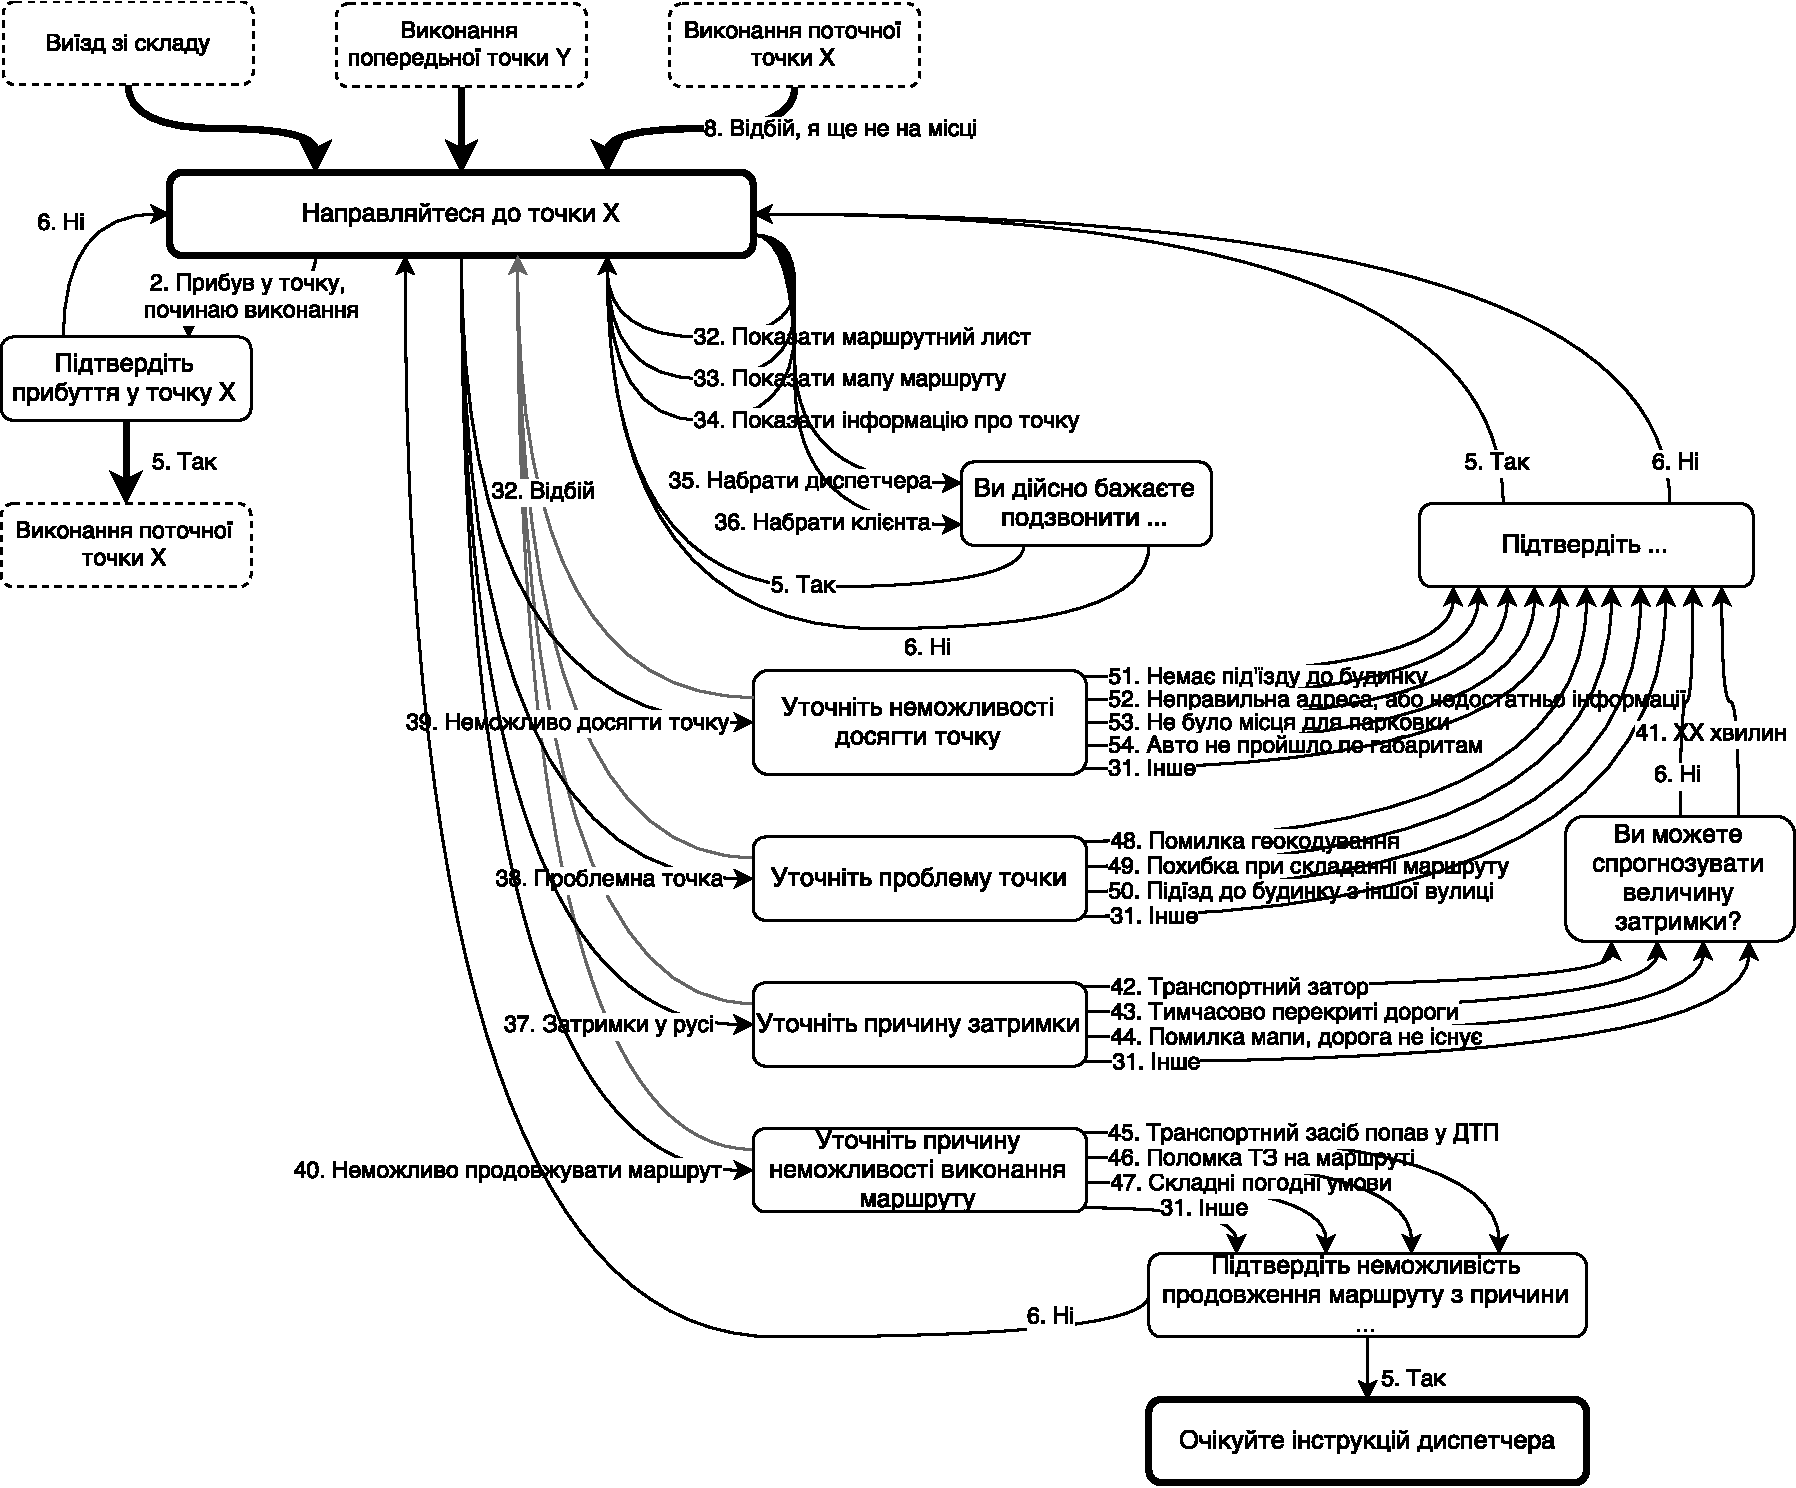
\includegraphics [width=.8\linewidth] {11_complete_road_scenario}
	\caption{Частина дерева сценаріїв етапу <<дорога>>}
	\label{img:11_complete_road_scenario}
\end{figure}

\begin{figure}
	\centering
	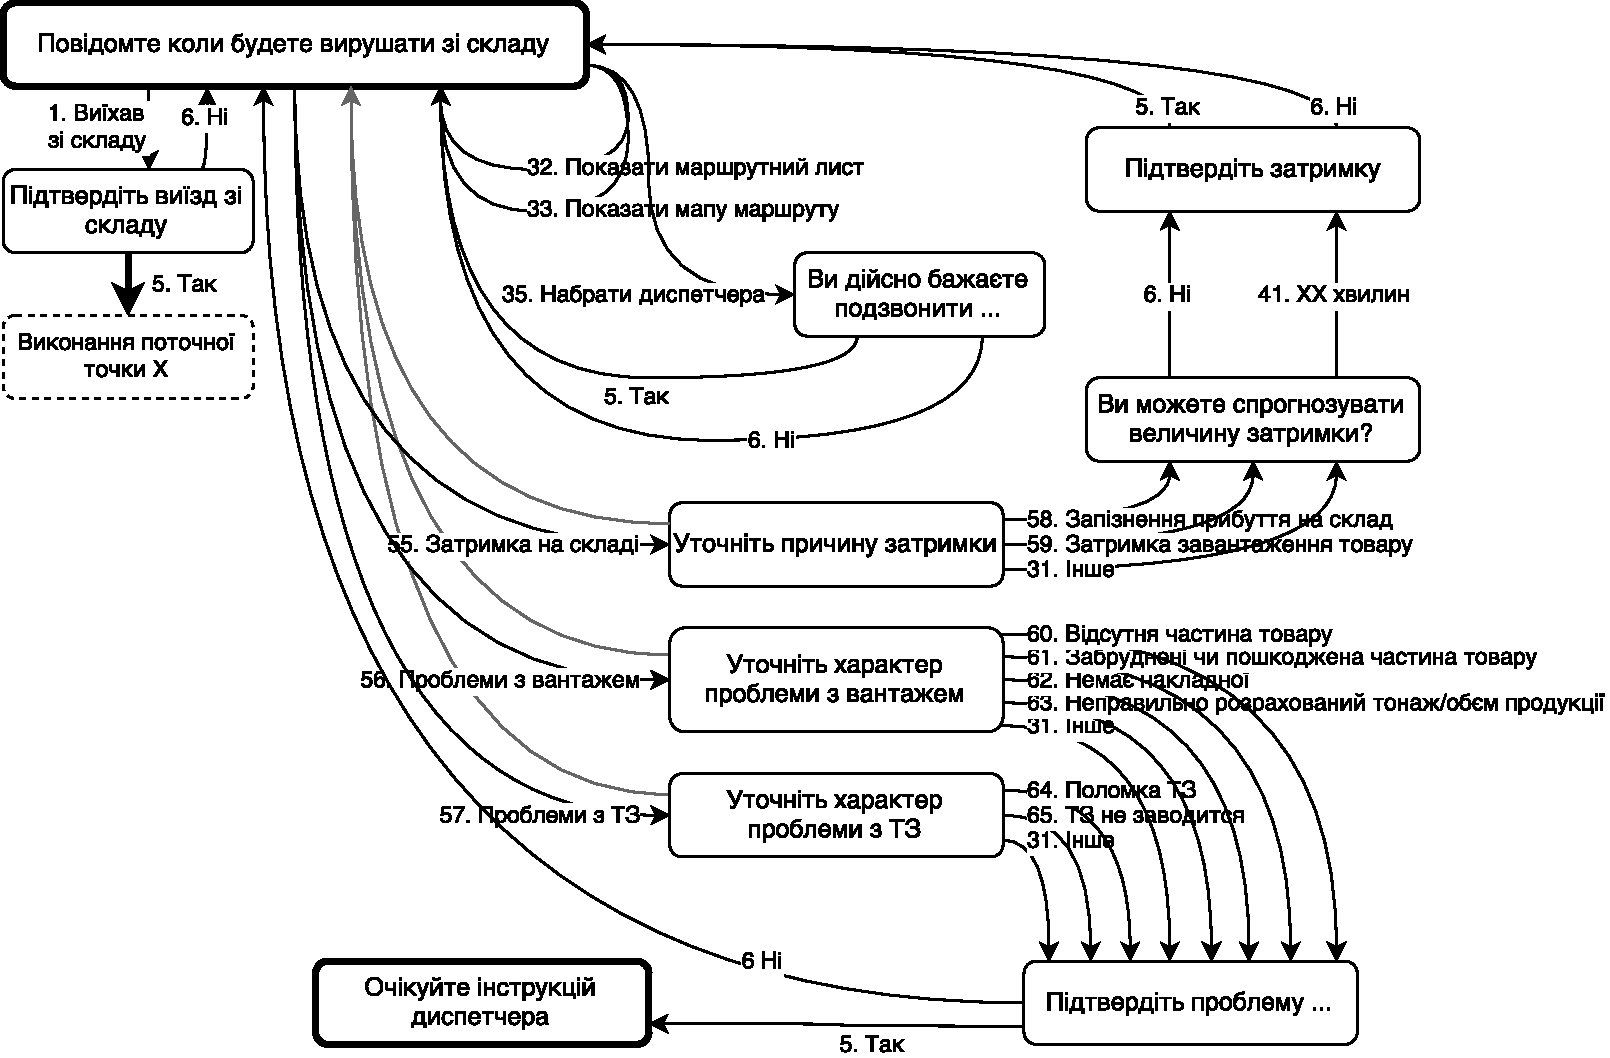
\includegraphics [width=.8\linewidth] {12_complete_depot_scenario}
	\caption{Частина дерева сценаріїв етапу <<склад>>}
	\label{img:12_complete_depot_scenario}
\end{figure}

Для виконання етапу «склад» субʼєктом дистрибуції – водієм при його голосовій взаємодії в системі диспетчерського контролю за рухом автотранспорту побудовано дерево сценаріїв етапу «склад», частину якого наведено на рис. \ref{img:12_complete_depot_scenario}.

У побудованому дереві сценаріїв етапу «склад» враховано причини затримки чи невиїзду зі складу з можливістю отримати подальші інструкції диспетчера для вирішення проблеми.

Повне дерево сценаріїв усіх етапів дистрибуції «склад – дорога – точка доставки» в моделі голосової взаємодії водія в системі диспетчерського контролю за рухом автотранспорту представлено на рис. \ref{img:13_complete_scenario_graph}.

\begin{figure}
	\centering
	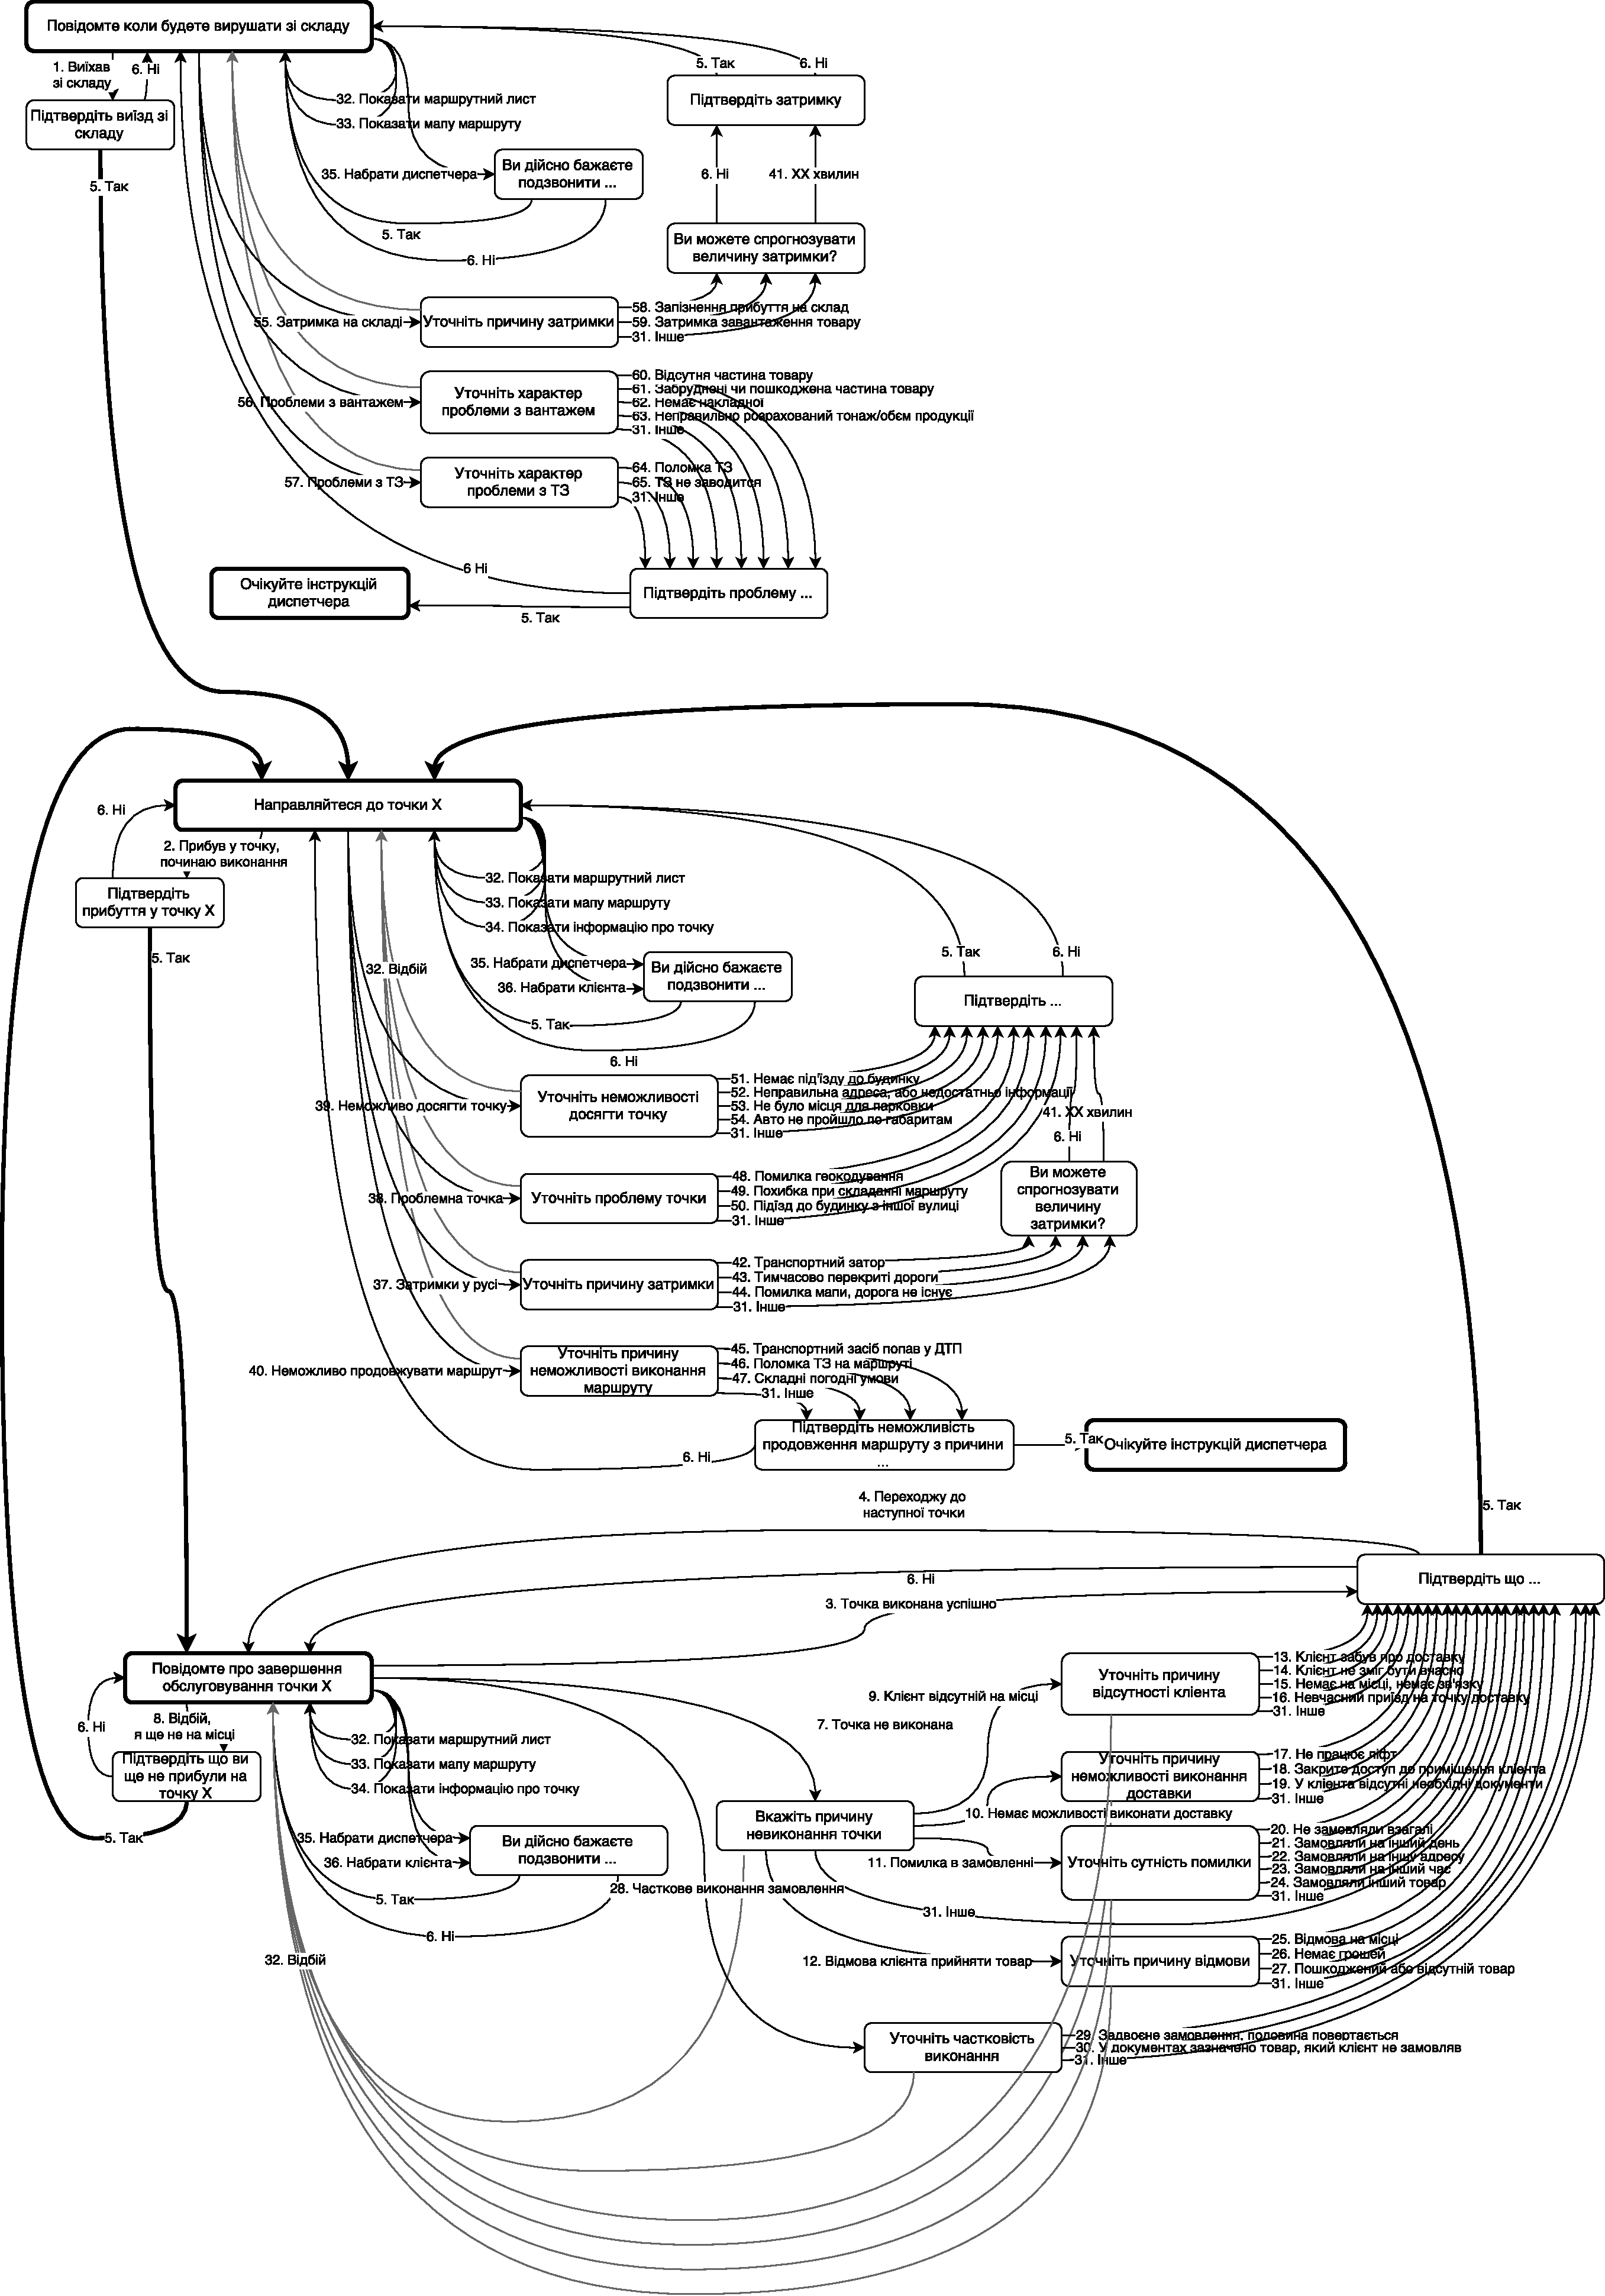
\includegraphics [width=1\linewidth] {13_complete_scenario_graph}
	\caption{Повне дерево сценаріїв всіх етапів} дистрибуції
	\label{img:13_complete_scenario_graph}
\end{figure}

\FloatBlock

У повному дереві сценаріїв усіх етапів дистрибуції (рис. \ref{img:13_complete_scenario_graph}) враховано всі можливі причини затримки або невиконання етапів «склад», «дорога», «точка доставки», а для таких випадків при неможливості виконання етапу існує вказівка (інструкції) диспетчера щодо подальших дій водія.

Наводимо повний перелік всіх унікальних стимулів з їх унікальними номерами в формі таблиці (табл. \ref{tbl:scenario_commands}).

\begin{mytable*}{ | c | l | }%
	{Різні варіанти стимулів з дерева сценаріїв}%
	{\label{tbl:scenario_commands}}%
	{№ & Варіанти стимулу}
	
	1 & Виїхав зі складу \\
	\hline
	2 & Прибув у точку, починаю виконання \\
	\hline
	3 & Точка виконана успішно \\
	\hline
	4 & Переходжу до наступної точки \\
	\hline
	5 & Так \\
	\hline
	6 & Ні \\
	\hline
	7 & Точка не виконана \\
	\hline
	8 & Відбій, я ще не на місці \\
	\hline
	9 & Клієнт відсутній на місці \\
	\hline
	10 & Немає можливості виконати доставку  \\
	\hline
	11 & Помилка в замовленні \\
	\hline
	12 & Відмова клієнта прийняти товар \\
	\hline
	13 & Клієнт забув про доставку \\
	\hline
	14 & Клієнт не зміг бути вчасно \\
	\hline
	15 & Клієнта немає на місці, немає звʼязку \\
	\hline
	16 & Невчасний приїзд на точку доставки \\
	\hline
	17 & Не працює ліфт \\
	\hline
	18 & Закрито доступ до приміщення клієнта \\
	\hline
	19 & У клиента відсутні необхідні документи \\
	\hline
	20 & Не замовляли товар взагалі \\
	\hline
	21 & Замовляли на інший день \\
	\hline
	22 & Замовляли на іншу адресу \\
	\hline
	23 & Замовляли на інший час \\
	\hline
	24 & Замовляли інший товар \\
	\hline
	25 & Відмова на місці \\
	\hline
	26 & Немає грошей \\
	\hline
	27 & Пошкоджений або відсутній товар \\
	\hline
	28 & Часткове виконання замовлення \\
	\hline
	29 & Задвоєне замовлення, половина товару повертається \\
	\hline
	30 & У документах зазначено товар, який клієнт не замовляв \\
	\hline
	31 & Інше \\
	\hline
	32 & Показати маршрутний лист \\
	\hline
	33 & Показати мапу маршруту \\
	\hline
	34 & Показати інформацію про точку \\
	\hline
	35 & Набрати диспетчера \\
	\hline
	36 & Набрати клієнта \\
	\hline
	37 & Затримки в русі \\
	\hline
	38 & Проблемна точка \\
	\hline
	39 & Неможливо дістатися точки \\
	\hline
	40 & Неможливо продовжувати маршрут \\
	\hline
	41 & \# хвилин \\
	\hline
	42 & Транспортний затор \\
	\hline
	43 & Тимчасово перекриті дороги \\
	\hline
	44 & Помилка мапи, дороги не існує \\
	\hline
	45 & Транспортний засіб потрапив у ДТП \\
	\hline
	46 & Поломка ТЗ на маршруті \\
	\hline
	47 & Складні погодні умови \\
	\hline
	48 & Помилка геокодування \\
	\hline
	49 & Похибка при складанні маршруту \\
	\hline
	50 & Підʼїзд до будинку з іншої вулиці \\
	\hline
	51 & Немає підʼїзду до будинку \\
	\hline
	52 & Неправильна адреса або недостатньо інформації \\
	\hline
	53 & Не було місця для парковки \\
	\hline
	54 & Авто не пройшло за габаритами \\
	\hline
	55 & Затримка на складі \\
	\hline
	56 & Проблеми з вантажем \\
	\hline
	57 & Проблеми з ТЗ \\
	\hline
	58 & Запізнення прибуття на склад \\
	\hline
	59 & Затримка завантаження товару \\
	\hline
	60 & Відсутня частина товару \\
	\hline
	61 & Забруднена або пошкоджена частина товару \\
	\hline
	62 & Немає накладної \\
	\hline
	63 & Неправильно розрахований тоннаж/обʼєм продукції \\
	\hline
	64 & Поломка ТЗ \\
	\hline
	65 & ТЗ не заводится \\
\end{mytable*}

Модель голосової взаємодії субʼєктів дистрибуції може бути представлена у вигляді орієнтовного графу $G$, що складається з множини вершин $V$ та множини ребер $E$:

\begin{align}
	G&=\langle V,E\rangle; \nonumber\\
	E&=\{\langle v_i,v_j\rangle | v \in V\}. \nonumber
\end{align}

При цьому існує відношення $f_R$ множини ребер до множини реакцій та відношення $f_C$ множини вершин до множини контекстів, такі що:

\begin{align}
	f_R&: E \rightarrow R,\quad R\subset\mathbb{N},\quad |R|\le|E|; \nonumber\\
	f_C&: V \rightarrow C,\quad C\subset\mathbb{N},\quad|C|\le|V|; \nonumber\\
	R_V(v_i) &= \{f_R(e)|\forall j:e=\langle v_i,v_j\rangle \in E\}; \nonumber\\
	\forall i,j: f_C(v_i)&=f_C(v_j) \iff R_V(v_i) = R_V(v_j), \nonumber
\end{align}

\noindent
де $R_V(v_i)$ --- множина реакцій, можливих у вершині $v_i$.

Адекватність розробленої моделі підтверджується її повною відповідністю статистичним даним інцидентів, зібраних за період упровадження системи, та експериментально --- шляхом порівняння результатів моделювання з використанням моделі та без її залучення.

\subsection{Виділення унікальних контекстів моделі голосової взаємодії}

Як було зазначено в підрозділі \ref{sect2_3}, кожна вершина в орієнтованому графі сценаріїв голосової взаємодії водія в системах диспетчерського контролю за рухом автотранспорту (рис. \ref{img:13_complete_scenario_graph}) позначає контекст голосової взаємодії, який може бути змодельовано окремо, а перелік ребер, що виходять з цієї вершини, обмежує можливий перелік голосових команд, які мають  бути розпізнані в цьому контексті.

Оскільки деякі контексти мають однаковий перелік можливих голосових команд, можемо не створювати для кожного з таких контекстів окрему модель, а повторно використовувати вже існуючі моделі контекстів з тим самим переліком голосових команд. Для визначення переліку необхідних моделей пронумеруємо всі контексти, представлені на дереві сценаріїв, залежно від переліку команд, які в них можуть бути розпізнані.

Повне дерево сценаріїв усіх етапів дистрибуції «склад – дорога – точка доставки» з вказівкою контекстів наведено на рис. \ref{img:14_complete_scenario_graph_contexts}. Використовуємо повне дерево сценаріїв, щоб знайти і пронумерувати унікальні контексти.

\begin{figure}
	\centering
	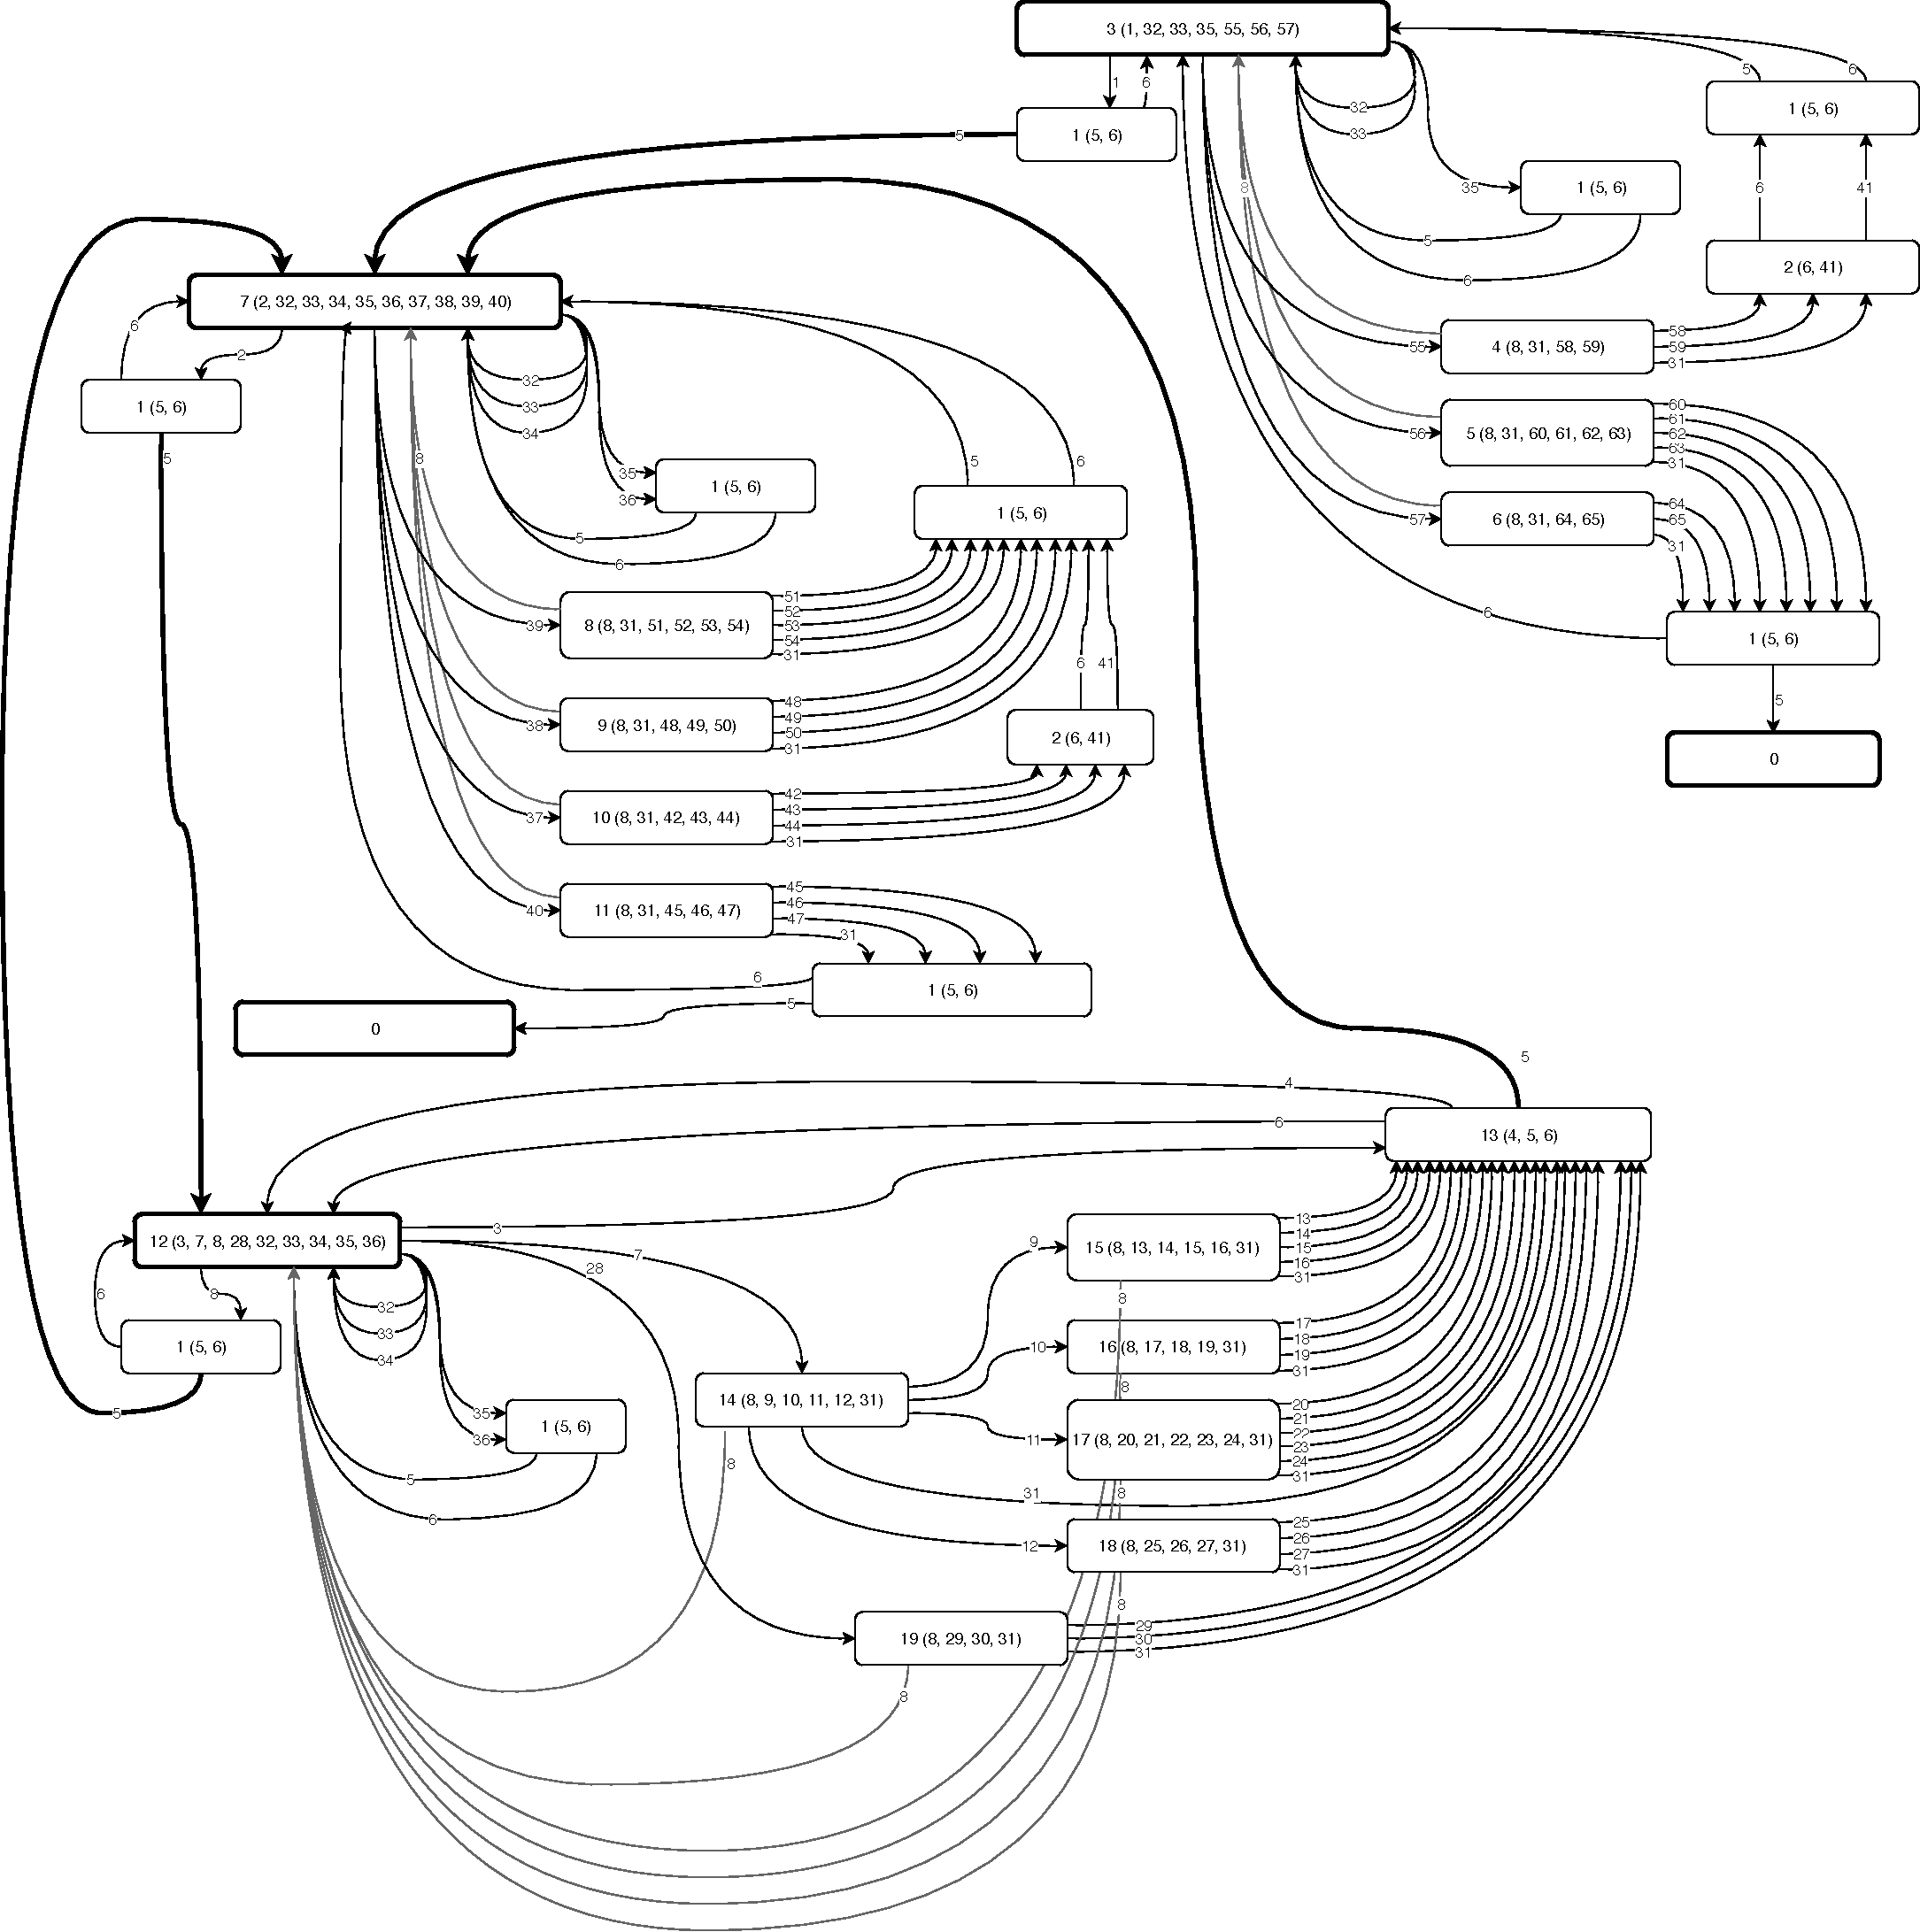
\includegraphics [width=1\linewidth] {14_complete_scenario_graph_contexts}
	\caption{Повне дерево сценаріїв усіх етапів дистрибуції з указанням контекстів}
	\label{img:14_complete_scenario_graph_contexts}
\end{figure}

Повне дерево сценаріїв усіх етапів дистрибуції «склад – дорога – точка доставки» з вказівкою контекстів (рис. \ref{img:14_complete_scenario_graph_contexts}) містить можливі реакції в них, тобто на кожний позначений контекст (табл. \ref{tbl:scenario_commands}) існує реакція, яку вказано в дужках на дереві сценаріїв.

У табл. \ref{tbl:context_reactions} представлено звʼязок контекстів і реакцій на них в моделі голосової взаємодії водія в системі диспетчерського контролю за рухом автотранспорту.

Відповідно до наведених блоків контексту в моделі голосової взаємодії водія в системі диспетчерського контролю за рухом автотранспорту прослідковується звʼязок можливих реакцій на них. Отже, відповідно до цього можна будувати систему формалізації голосової інформації.

\begin{mytable}{ | c | l | }%
	{Перелік контекстів та можливих реакцій у них}%
	{\label{tbl:context_reactions}}%
	{№ & Можливі реакції}
	
	1 & 5, 6 \\
	\hline
	2 & 6, 41 \\
	\hline
	3 & 1, 32, 33, 35, 55, 56, 57 \\
	\hline
	4 & 8, 31, 58, 59 \\
	\hline
	5 & 8, 31, 60, 61, 62, 63 \\
	\hline
	6 & 8, 31, 64, 65 \\
	\hline
	7 & 2, 32, 33, 34, 35, 36, 37, 38, 39, 40 \\
	\hline
	8 & 8, 31, 51, 52, 53, 54 \\
	\hline
	9 & 8, 31, 48, 49, 50 \\
	\hline
	10 & 8, 31, 42, 43, 44  \\
	\hline
	11 & 8, 31, 45, 46, 47 \\
	\hline
	12 & 3, 7, 8, 28, 32, 33, 34, 35, 36 \\
	\hline
	13 & 4, 5, 6 \\
	\hline
	14 & 8, 9, 10, 11, 12, 31 \\
	\hline
	15 & 8, 13, 14, 15, 16, 31 \\
	\hline
	16 & 8, 17, 18, 19, 31 \\
	\hline
	17 & 8, 20, 21, 22, 23, 24, 31 \\
	\hline
	18 & 8, 25, 26, 27, 31 \\
	\hline
	19 & 8, 29, 30, 31 \\
\end{mytable}

\subsection{Створення моделі формалізації голосової інформації для кожного контексту голосової взаємодії}

Розглянемо будь-який контекст голосової взаємодії водія в системах диспетчеризації автотранспорту. Для формалізації голосової інформації в цьому контексті необхідно створити модель класифікації голосових висловлювань водія, що відповідає можливому переліку голосових команд у моделі голосової взаємодії.

Представимо перелік можливих голосових команд як множину:

\[
A = {A_i | i=\overline{1..n}},
\]

\noindent
де $A$ --- множина голосових команд $A_i$, а $n$ --- кількість можливих голосових команд у контексті, що розглядається.

Тоді для кожного голосового висловлювання $B$, сказаного водієм, існує ймовірність $p(A_i/B)$, що це висловлювання було командою $A_i$. Задача формалізації голосової інформації полягає у визначенні того, яка з команд є найбільш ймовірною.

Для вирішення цієї задачі пропонується дуальна система класифікації, яка може бути налаштована на предметну область і використовувати метод інтелектуальних рефлекторних систем або метод згорткових нейронних мереж залежно від того, який з них показує кращі результати.

У даному підрозділі представлено розроблене дерево сценаріїв усіх етапів дистрибуції «склад – дорога – точка доставки» як модель голосової взаємодії водія в системах диспетчерського контролю за рухом автотранспорту та визначено перелік контекстів та можливих реакцій на них.

\section{Дуальний метод формалізації голосової інформації в системах диспетчерського контролю за рухом автотранспорту} \label{sect3_4}

\subsection{Інтелектуальні рефлекторні системи}

Для формалізації голосової інформації можна використати систему з двох основних модулів: автоматичного фонетичного стенографа і ядра рефлекторної системи голосового управління (РСГУ), поточна реалізація яких визначає умови їх використання в моделі голосової взаємодії водія при диспетчерському контролі за рухом автотранспорту (рис. \ref{img:rsgu_struct}).

\begin{figure}
	\centering
	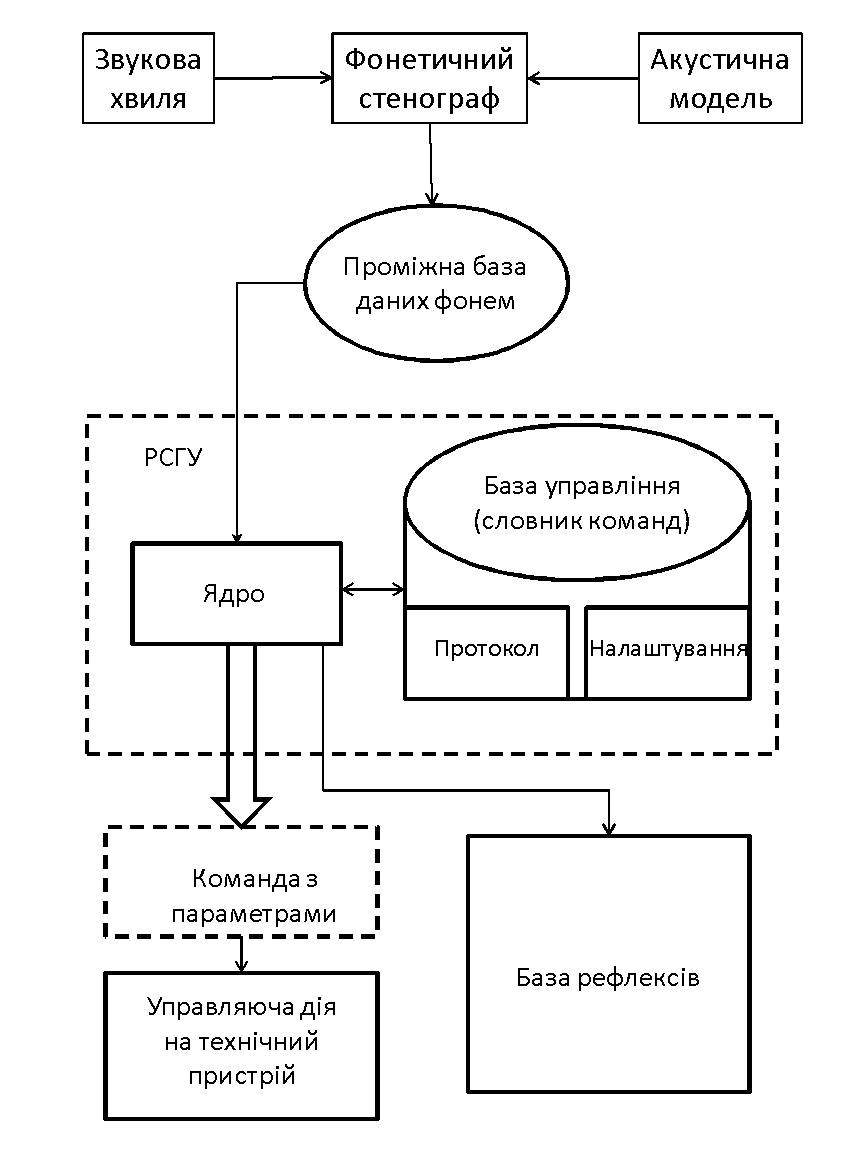
\includegraphics [width=.5\linewidth] {rsgu_struct}
	\caption{Структура системи формалізації голосової інформації в моделі голосової взаємодії водія при диспетчерському контролі за рухом автотранспорту}
	\label{img:rsgu_struct}
\end{figure}

Застосування алгоритму фонетичного стенографа дає змогу будувати послідовність контекстів для мовного сигналу без використання будь-якого словника. З цією метою будується деяка генеративна граматика, яка може синтезувати всі можливі модельні сигнали безперервної мови для будь-якої послідовності фонем. У межах побудованої моделі розробляється алгоритм пофонемного розпiзнавання для невідомого сигналу з використанням контекстів та можливих реакцій на них.

Виконання фонетичного стенографу \cite{Pylypenko_2008} здійснено у вигляді бінарного додатку, набору бібліотек і конфігураційних файлів для платформи Windows, а саме ядро РСГУ, яке виконує реалізацію інтроформаційного методу вироблення рефлексів, розроблено і виконано в середовищі MS Access на всіх операційних системах сімейства Windows.

У системі формалізації голосової інформації, що розглядається (рис. \ref{img:rsgu_struct}), вхідною інформацією виступає голосова команда, яка може бути представлена звуковою хвилею; вихідною ж інформацією виступатиме процес керуючого впливу на обʼєкт управління, тобто відбуватиметься виконання розпізнаної команди відповідно до попередньо заданих голосом параметрів.

Сама система формалізації голосової інформації в процесі роботи генеруватиме потрібні візуальні і голосові інформаційні повідомлення водію, а це, у свою чергу, надаватиме можливість відслідковувати процес розпізнавання команд, реакції на них і, крім того, даватиме змогу в реальному масштабі часу змінювати поведінку системи в разі потреби.

Розглянемо схему роботи системи формалізації голосової інформації в моделі голосової взаємодії водія при диспетчерському контролі за рухом автотранспорту. Водій у вільній формі озвучує необхідні для нього дії системи. Наприклад, по відношенню до голосового управління системою це може бути: «Показати маршрутний лист», або «Показати мапу маршруту», або «Показати інформацію про точку». Програмна платформа системи формалізації голосової інформації в моделі голосової взаємодії водія при диспетчерському контролі за рухом автотранспорту передає необхідну команду на технічний пристрій або озвучує водієві затребувану  ним  інформацію. Під час  навчання водій сам виконує відповідну дію і у системи виробляється рефлекс на подібне звернення. Якщо водії говорять «по-різному», то виробляється стійкий рефлекс саме на інформативну частину голосової команди. При цьому в системі формалізації голосової інформації в моделі голосової взаємодії водія при диспетчерському контролі за рухом автотранспорту наявні такі стани, команди та засоби:

1. \textbf{Звукова команда}. Водій голосом звертається з проханням до технічного пристрою.

Вихідною інформацією є звукова хвиля.

Наведемо приклад для даної команди: покажи мені, будь ласка, інформацію про точку.

2. \textbf{Акустична модель}. Включає статистичний опис розпізнавання мови і особливостей мови водія. Статистичний опис формується в процесі навчання налаштуванням на водіїв. Як акустичні використовуються приховані Марківські моделі. 65 українських контекстно-незалежних фонем моделюються трьома станами Марківського ланцюга без пропуску.

Створення словника транскрипцій акустичних моделей відбувається автоматично з орфографічного словника з використанням контекстно-незалежних правил.

3. \textbf{Фонетичний стенограф}. Служить для перетворення вхідного оцифрованого звукового сигналу, що містить усне мовлення (акустичної моделі), в набір фонем.

Алгоритм фонетичного стенографа дає змогу будувати послідовність фонем для мовного сигналу без використання будь-якого словника. З цією метою будується деяка генеративна граматика, яка може синтезувати всі можливі модельні сигнали безперервної мови для будь-якої послідовності фонем. У межах побудованої моделі розробляється алгоритм пофонемного розпiзнавання для невідомого сигналу. Використовуються ті самі контекстно незалежні моделі фонем, як і в базовому розпізнавачі.

Надійність виявлення фонеми на правильному місці для відомої реалізації дорівнює приблизно 70\%.

Вихідна інформація: проміжна база даних фонем – результат розпізнавання вхідних звукових хвиль.

4. \textbf{Ядро РСГУ}. Призначено для моделювання системи голосового управління технічним пристроєм. Містить програмну реалізацію інтроформаційного методу, а також алгоритмів виділення комбінацій фонем і навчання (накопичення статистики). Інформаційна база управління містить словник команд, протокол роботи, налаштування системи.

5. \textbf{Команда з параметрами}. Результатом роботи системи є команда з параметрами, яку необхідно реалізувати технічному пристрою.

Вихідною інформацією є виконувана команда.

Приклад: водій – Найдьонов, команда – Х хвилин, рівень – десятки, десятки хвилин – 10, одиниці хвилин – 8.

6. \textbf{Керуючий вплив}. Містить програмну реалізацію алгоритму управління технічним пристроєм.

Вхідною інформацією є формалізована команда з відповідними параметрами.

Результатом керуючого впливу є зміна параметрів самого технічного пристрою.

Прикладом керуючого впливу може бути інформація про наступний час виконання.

Система формалізації голосової інформації в моделі голосової взаємодії водія при диспетчерському контролі за рухом автотранспорту відрізняється простотою і, в даному випадку, реалізує рефлекторну модель поведінки, яку наведено на рис. \ref{img:rsgu_scheme}

\begin{figure}
	\centering
	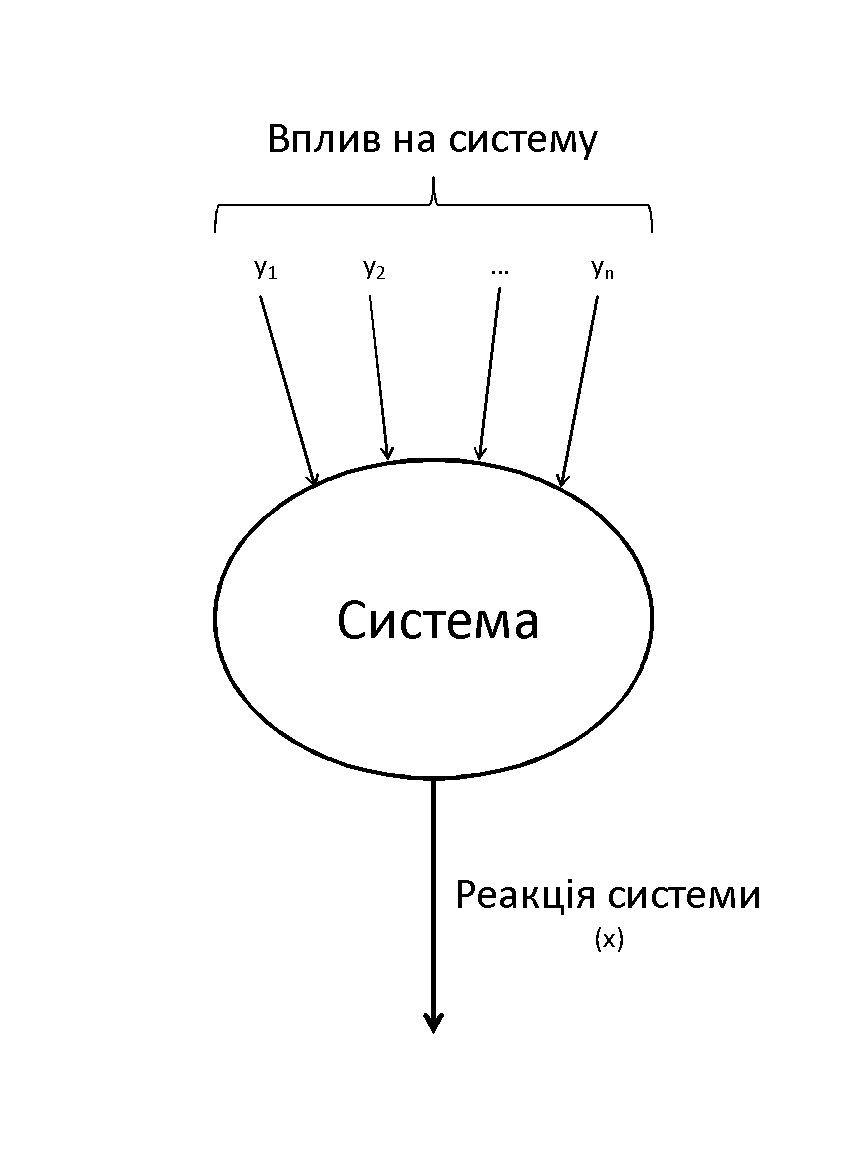
\includegraphics [width=.5\linewidth] {rsgu_scheme}
	\caption{Схема реакції системи формалізації голосової інформації в моделі голосової взаємодії водія при диспетчерському контролі за рухом автотранспорту на несилові впливи}
	\label{img:rsgu_scheme}
\end{figure}

Система формалізації голосової інформації в моделі голосової взаємодії водія при диспетчерському контролі за рухом автотранспорту функціонує в режимі навчання і режимі управління. У режимі навчання відбувається формування бази рефлексів.
У режимі управління РСГУ відбувається вироблення реакції на звернення водія. Також у цьому режимі відбувається реалізація режиму самонавчання – для випадку, коли отримана реакція не задовольняє водія.

Основною частиною системи формалізації голосової інформації в моделі голосової взаємодії водія при диспетчерському контролі за рухом автотранспорту є база рефлексів. База рефлексів містить статистику вхідних впливів (комбінацій фонем) і реакцій системи, розділених на класи: водій, команда, рівень числа, десятки, одиниці (рис. \ref{img:rsgu_base}).

\begin{figure}
	\centering
	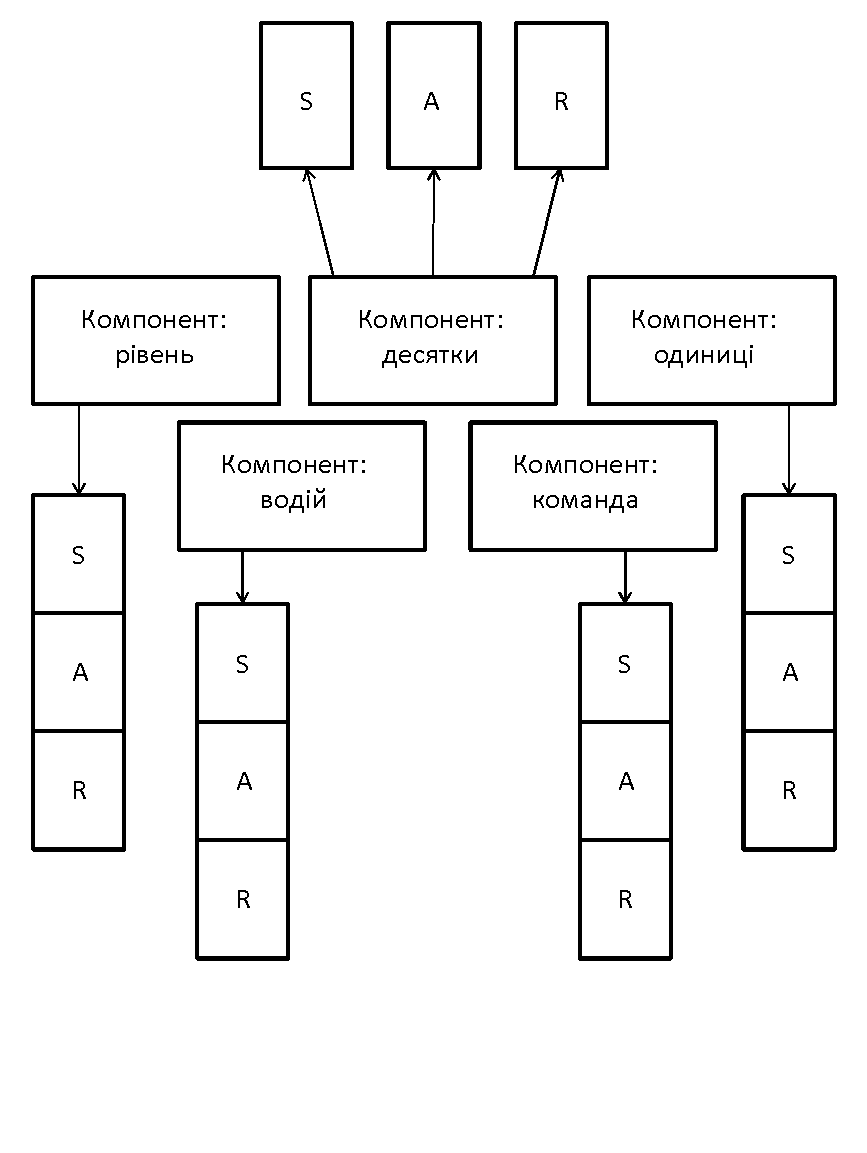
\includegraphics [width=.5\linewidth] {rsgu_base}
	\caption{Структура бази рефлексів системи формалізації голосової інформації}
	\label{img:rsgu_base}
\end{figure}

Реалізація кожного класу рефлексів відбувається в кожному окремому компоненті системи формалізації голосової інформації в моделі голосової взаємодії водія при диспетчерському контролі за рухом автотранспорту. Представлення кожного компоненту системи здійснюється у вигляді окремого «інтроформаційного» нейрона.

На вході системи задається повний вхідний набір фонем та/або реакція інших «інтроформаційних» нейронів, на виході – вироблена реакція нейронів, яка надходить на інші «інтроформаційні» нейрони або безпосередньо на технічний пристрій.

У кожному компоненті системи формалізації голосової інформації в моделі голосової взаємодії водія при диспетчерському контролі за рухом автотранспорту інформація зберігається в таких таблицях:

\begin{itemize}
	\item S – таблиця з комбінацією фонем, в якій знаходяться та зберігаються всі комбінації послідовних фонем з довжинами від 2-х до 10 символів з інформацією про те, скільки разів вони траплялися;
	\item R – таблиця реакції РСГУ, в якій міститься перелік дій, які необхідно виконати РСГУ або технічному пристрою, частота користування і визначеність даної реакції. Реакція типу «Не знаю» забезпечує відкритість системи;
	\item А – таблиця, призначена для встановлення звʼязку вищенаведених таблиць S і R. Містить інформацію про те, яка реакція і скільки разів була затребувана у випадку, коли на вході був деякий набір фонем. Крім того, таблиця містить відомості про визначеність реакції, що повʼязана з цим набором фонем.
\end{itemize}

При режимі навчання у вищенаведених таблицях відбувається накопичення інформації про звʼязок вхідних фраз (контекстів) і реакцій системи формалізації голосової інформації в моделі голосової взаємодії водія при диспетчерському контролі за рухом автотранспорту. У процесі роботи системи отримана інформація використовується далі в режимі управління для вироблення реакцій на відповідні звернення водія на основі інтроформаційного методу \cite{Teslia_2010}. При цьому алгоритм реалізації режиму управління в системі має таку послідовність:

\begin{itemize}
	\item перший етап. Старт алгоритму.
\end{itemize}

При надходженні на вхід системи потоку фонем виділяються фрагменти (набори) множиною M, що містять від 2 до 4 символів, які стоять поруч;

\begin{itemize}
	\item другий етап. Відбір класу команд.
\end{itemize}

З таблиці S здійснюється відбір записів, які відповідають сформованим наборам фонем, що належать до множини M.
На основі інтроформаційного методу відбувається обчислення визначеності реакцій (команд), що містяться в таблицях A і R. Команда, що має найбільшу визначеність, вибирається для реалізації;

\begin{itemize}
	\item третій етап. Якщо в команді є звернення до числового значення (знак \#), розглядаються класи рівня числа (десятки, одиниці).
\end{itemize}

Клас рівня числа. З таблиці S здійснюється відбір записів, які відповідають сформованим наборам фонем (що входять у множину M). З використанням таблиць A і R відповідно до інтроформаційного методу обчислюється визначеність рівня числа. Варіанти: немає десятків хвилин (числа від 0 до 9), є десятки хвилин (числа більше 9).

Якщо рівень числа «Є десятки хвилин», то активізуються таблиці, що входять у клас десятків хвилин. З таблиці S здійснюється відбір записів, які відповідають сформованим наборам фонем (що входять у множину M). З використанням таблиць A і R відповідно до інтроформаційного методу обчислюється визначеність номера десятка. Якщо десяток не визначений, у команду вставляється знак «?».

Клас одиниць хвилин. З таблиці S здійснюється відбір записів, які відповідають сформованим наборам фонем (що входять в множину M). Використовуючи таблиці A і R, відповідно до інтроформаційного методу обчислюється визначеність другий цифри в числі. Якщо цифра не визначена, в команду вставляється знак «?»;

\begin{itemize}
	\item четвертий етап. Завершення алгоритму.
\end{itemize}

Отже, метод інтелектуальних рефлекторних систем для формалізації голосової інформації в системах диспетчерського контролю за рухом автотранспорту можна представити таким чином:

\begin{enumerate}
	\item запис фрази, вимовленої водієм; $A_i=<a_1,a_2,...,a_n>; t=\frac{n}{s}; s=16 \textbf{(kHz)};$
	\item перетворення записаної фрази на фонетичний текст за допомогою фонемного стенографа; $P_i=S(A_i); P=<p_1,p_2,...,p_k>; p_i \in F;$
	\item класифікація фонемної репрезентації голосової команди; $y_i=C_c(P_i)$
	\begin{enumerate}
		\item розбиття фонетичного тексту на N-грами фонем різної довжини;
		\item розрахунок інтроформаційного впливу кожного N-граму фонем на можливі команди у вибраному контексті;
		\item вибір команди з найбільшою ймовірністю;
	\end{enumerate}
	\item виконання відповідної реакції (озвучення відповіді, виконання команди та/або відправка структурованих даних диспетчеру);
	\item переключення контексту на новий, відповідний до вибраної реакції; $c_{i+1} = f(c_i, y_i)$
	\item очікування та запис наступної фрази.
\end{enumerate}

{\settowidth{\leftskip}{Де:\ }
	
	$A_i$ --- цифровий аудіозапис команди водія довжиною $t$ секунд,
	
	$n$ --- кількість семплів аудіосигналу,
	
	$s$ --- частота дискретизації аудіосигналу,
	
	$P_i$ --- представлення команди водія у вигляді фонемного тексту --- кортежу фонем довжини $k$,
	
	$F$ --- множина фонем української мови,
	
	$S$ --- фонемний стенограф,
	
	$y_i$ --- реакція з моделі голосової взаємодії субʼєктів дистрибуції, яка відповідає вимовленій команді,
	
	$C_c$ --- класифікатор фонемної репрезентації голосових команд відповідно до поточного контексту $c_i$,
	
	$f$ --- функція визначення наступного контексту залежно від поточного контексту $c_i$ та вибраної реакції $y_i$.
	
}

Таким чином, у кожний компонент системи надходить весь вхідний набір фонем без виділення слів, команд, пропозицій тощо. Результат роботи даного методу такий самий, як і роботи головного мозку людини. Тобто, слухаючи усне мовлення, або читаючи лист, людина, не виокремлюючи букви і слова, розпізнає сенс. Те саме відбувається і в рефлекторній системі голосового управління. При цьому не потрібно створювати ніяких словників, виконувати морфологічний, синтаксичний, семантичний аналіз тексту, а також виділяти слова і команди; виникнення реакції відбувається на звуковий потік, з якого система формалізації голосової інформації в моделі голосової взаємодії водія при диспетчерському контролі за рухом автотранспорту, як і людина, сама «вміє виділяти» інформативну частину за максимальною визначеністю \cite{Teslia_2013}.

Для підвищення ефективності розпізнавання було запропоновано удосконалену схему системи формалізації голосової інформації в моделі голосової взаємодії водія в дистрибуції (рис. \ref{img:rsgu_struct_new}), яка включає моделювання за кожним контекстом із моделі голосової взаємодії та дуальну систему класифікації фонемної репрезентації голосових команд, що дає змогу вибрати кращий метод класификації залежно від предметної області.

\begin{figure}[h!]
	\centering
	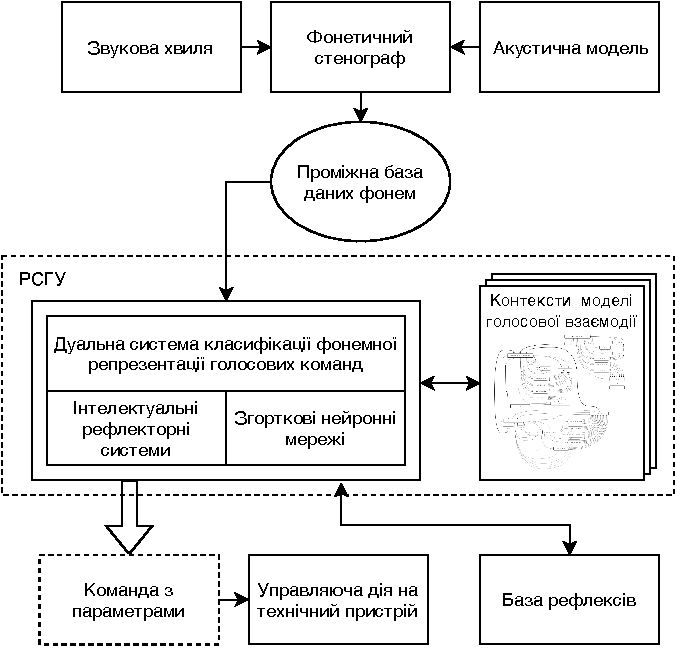
\includegraphics [width=.6\linewidth] {rsgu_struct_new}
	\caption{Удосконалена схема системи формалізації голосової інформації в моделі голосової взаємодії водія при диспетчерському контролі за рухом автотранспорту}
	\label{img:rsgu_struct_new}
\end{figure}

У якості альтернативного класифікатора фонетичного тексту голосової команди запропоновано використання методу згорткових нейронних мереж, що широко використовується в різноманітних задачах класифікації звукових даних \cite{Weisskirchen_2017,Boddapati_2017,Chowdhury_2018} та природномовних текстів \cite{Kim_2014,Britz_2015_2,Britz_2015,Kim_2016,Zhang_2015_2,Zhang_2015,Santos_2014}.

\subsection{Згорткові нейронні мережі}

У даному випадку система формалізації голосової інформації в моделі голосової взаємодії водія при диспетчерському контролі за рухом автотранспорту аналогічно до РСГУ, складається з двох частин: фонемний стенограф та сама згорткова нейронна мережа (ЗНМ), яка працює з фонемами.
ЗНМ для роботи з фонемами найбільше нагадує ЗНМ у задачі класифікації текстів \cite{Kim_2014}, але працює з «текстом» не по словах, а пофонемно, що схоже на роботу з текстом посимвольно \cite{Zhang_2015}.

ЗНМ дуже схожі на звичайні нейронні мережі: вони також побудовані на основі нейронів, які характеризуються постійно змінюваною вагою і зсувами. Кожен нейрон отримує деякі вхідні дані, виконує скалярне перетворення інформації і, в окремих ситуаціях, супроводжується нелінійністю. Як і у випадку зі звичайними нейронними мережами, вся ЗНМ моделює одну диференційовану функцію внеску: з одного боку, це необроблені фонеми, з іншого – висновок щодо класу або групи ймовірних класів, які характеризують фонему. Також наявна функція втрати на останньому (повністю підключеному) шарі ЗНМ.

Архітектура ЗНМ робить явне припущення виду «вхідні дані є фонеми», що дає змогу закодувати певні властивості під архітектуру. Завдяки цій особливості попереднє оголошення можна реалізувати більш ефективно, зменшуючи при цьому кількість параметріу в мережі.

Нейронні мережі отримують вхідні дані (один вектор), після чого трансформують інформацію, проводячи її через ряд прихованих шарів \cite{Kim_2014, Zhang_2015}. Кожен прихований шар складається з множини нейронів, де всякий нейрон має стійкий звʼязок з усіма нейронами в попередньому шарі і де нейрони в функції одного шару повністю незалежні один від одного і не мають спільних звʼязків. Останній повнозвʼязний шар називається вихідним шаром і в налаштуваннях класифікації він демонструє число класів.

На відміну від звичайних повнозвʼязних нейронних мереж, згорткові нейронні мережі враховують просторову структуру даних, тобто, той факт, що фонеми, які знаходятся поряд, мають більший звʼязок між собою і спільний вплив на результуючу змінну.

У роботі, за основу реалізації було взято реалізацію з відкритим вихідним кодом \cite{Britz_2015} на мові Python з використанням TensorFlow.

Структура нейронної мережі може бути представлена у такий спосіб (рис. \ref{img:cnn-struct}).

\begin{figure}
	\centering
	\subbottom[\label{img:cnn-struct1}]{%
		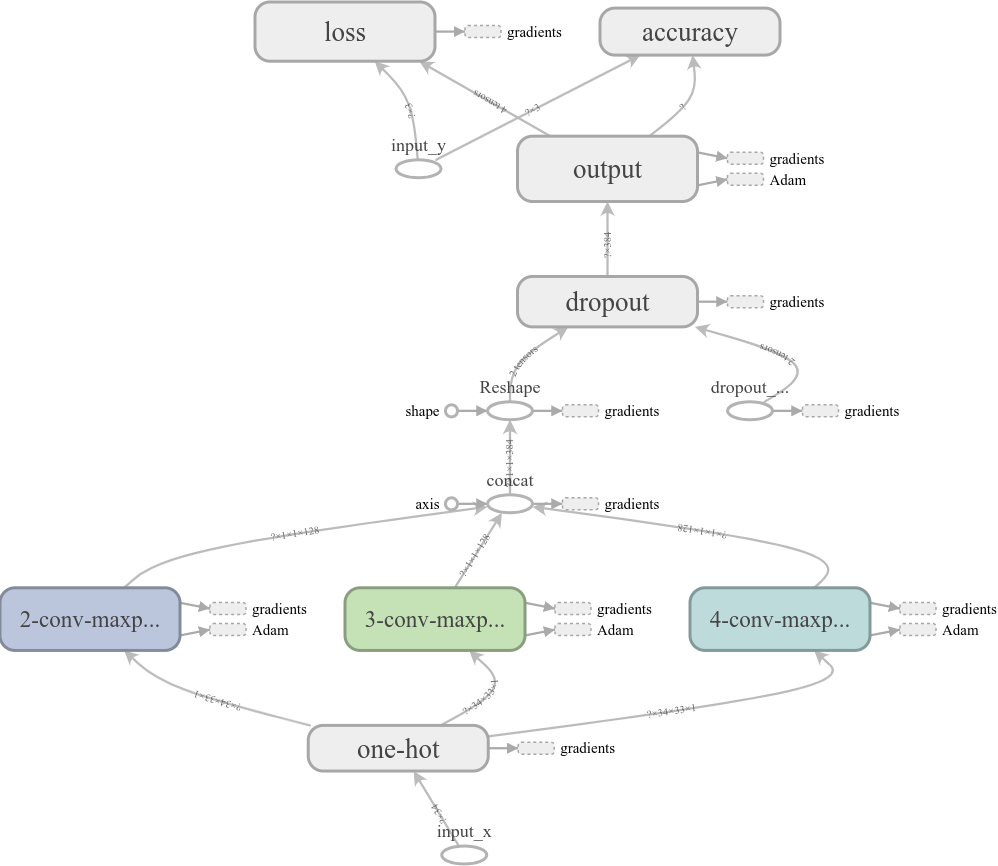
\includegraphics[width=.7\linewidth]{cnn_1}}
	\hfill
	\subbottom[\label{img:cnn-struct2}]{%
		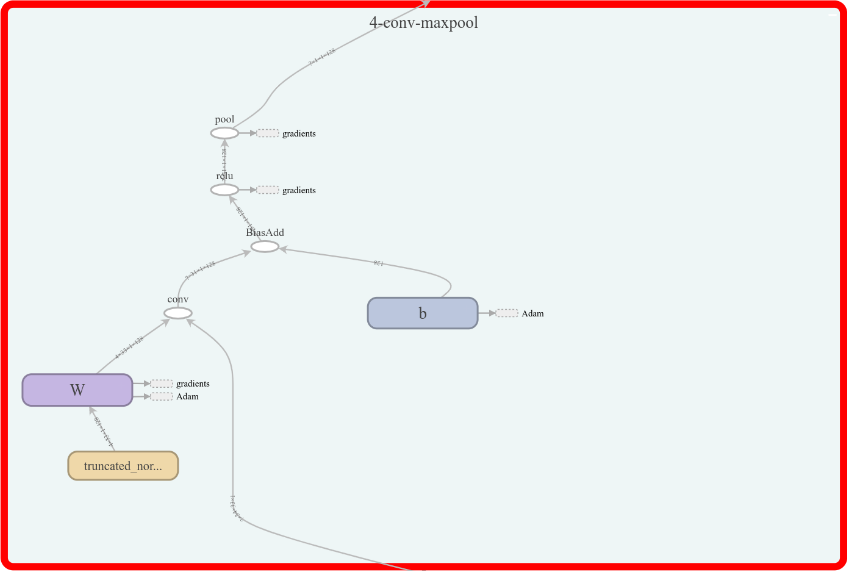
\includegraphics[width=.25\linewidth]{cnn_2}}
	\caption{Структура згорткової нейронної мережі (\subcaptionref{img:cnn-struct1}) та деталізація її згорткового шару (\subcaptionref{img:cnn-struct2})}
	\label{img:cnn-struct}
\end{figure}

Фонеми представлено у вигляді one-hot вектору. Фрази нормалізовано за максимальною довжиною з використанням вектора з усіма нулями в якості заповнювача.

На відміну від випадку роботи за словами, у ЗНМ класифікації фонем вкладений шар (embedding layer) відсутній, оскільки потужність множини фонем набагато нижча, ніж потужність множини слів, що робить такий шар не необхідним. З іншого боку, деякі фонеми схожі на інші, деякі --- ні, тому використання вкладень може бути доцільним для передачі цієї схожості, а не тільки для зниження розмірності. Навчання вкладеного шару потребує великого обʼєму вхідних даних, тому в даній роботі розглядатися не буде.

Використовується комбінований згортковий шар (convolution layer), який складається з кількох паралельних одновимірних шарів з різними варіантами кроку фільтра.

Для агрегації кожного зі згорткових шарів використовується агрегаційний шар (pooling layer) з вибором одного максимального значення (1-max-pooling).

Виходи агрегаційних підшарів різного розміру кроку згортки комбінуються в один вектор значень.

У якості повнозвʼязного шару використовується класичний перцептрон, який може мати активаційну функцію у вигляді не спадаючих диференційованих функцій, що діють на множині дійсних чисел. У нашому випадку для функції активації використаємо ReLU:

\[
h(a) = \max(0, a),
\]

\noindent
де $a=WX+b$

Застосування у якості функції активації ReLU дозволяє забезпечити головні переваги, які надають можливість здійснити пришвидшення навчання нейронної мережі через розрідженість та меншу величину ймовірності розмиття градієнту порівняно з іншими активаційними функціями. Виникнення розрідженості відбувається при значеннях a < 0. Для більшої кількості нейронів з ReLU-активацією в шарі характерна більша розрідженість отриманого результату.

Для зниження ефекту перенавчання використовується Dropout шар.

Традиційно для задач класифікації в якості функції втрат використовується кросс-ентропія. Отже, наступний наш крок --- мінімізація різниці між виходом нейронної мережі і відповідною фонемою (контекстом). Різницею як раз і буде величина кросс-ентропії, яка визначається за формулою:

\[
D(\hat{y},y)=-\sum_j y_i \ln \hat{y}_i
\]

Для навчання використовується Adam-алгоритм зворотного розповсюдження помилки із стохастичним градієнтним спуском, який дає змогу регулювати величину швидкості навчання залежно від параметрів з виконанням більших оновлень для 32-х або 16-ти параметрів, які трапляються рідко, і маленьких оновлень --- для параметрів, які трапляються частіше \cite{Kingma_2014}. У даному методі використовуються накопичені значення градієнтів, отримані на попередніх кроках, і накопичені значення квадратів градієнтів. Сам процес накопичення відбувається на основі експоненціального розпаду середніх значень (EDAverage). Значення, отримані на останньому кроці, здійснюють найбільший внесок у сумарне вихідне значення порівняно із значеннями градієнтів, отриманими на перших кроках:

\[
\bar{m_t}=\beta_1m_{t-1}+(1-\beta_1)g_t;
\]

\[
\bar{v_t}=\beta_2v_{t-1}+(1-\beta_2)g^2_t,
\]

\noindent
де $\bar{m_t}$ – середня оцінка першого моменту; $\bar{v_t}$ – середня оцінка другого моменту.

Оскільки у вищенаведених формулах констатація величин $\bar{m_t}$ і $\bar{v_t}$ може бути ініціалізована нулями, то виходить, вони мають тяжіння до нулів. Таке тяжіння відчутно проявляється на початкових кроках і у випадках, коли величина коефіцієнтів розпаду приймає мале значення ($\beta_1$ і $\beta_2$). Для вирішення цієї проблеми на значення моментів накладається штраф:

\[
\hat{m}_t=\frac{m_t}{1-\beta_1^t};
\]

\[
\hat{v}_t=\frac{v_t}{1-\beta_2^t}.
\]

Величини отриманих значень використовуються в процесі оновлення параметрів на основі формули:

\[
\Theta_{t+1}=\Theta_t-\frac{\eta}{\sqrt{\hat{v}_t}+\varepsilon}\hat{m}_t.
\]

Отже метод згорткових нейронних мереж для класифікації фонемної репрезентації голосових команд як частину дуальної системи формалізації голосової інформації в системах диспетчерського контролю за рухом автотранспорту можна сформулювати таким чином:

\begin{enumerate}
	\item представлення кожної фонеми у вигляді one-hot вектору;
	\item розрахунок одновимірного згорткового шару з фільтрами розмірами 2, 3 та 4 і кроком 1;
	\item розрахунок агрегаційного шару виділенням максимального значення кожного фільтру;
	\item конкатенація результатів обрахунку всіх фільтрів;
	\item розрахунок повнозвʼязного шару з функцією активації ReLU та нормалізацією Dropout;
	\item розрахунок точності та функції втрат.
\end{enumerate}

\subsection{Представлення інтелектуальних рефлекторних систем у термінах згорткових нейронних мереж}

Якщо детально розглянути ядро розрахунків РГСУ (розд. \ref{subsect2_4_2}), то виявиться, що воно дуже нагадує повнозвʼязний шар нейронної мережі. Умовна ймовірність вибору реакції $A_i$ при існуванні впливу $B_j$ ($p(A_i/B_j)$) відповідає вагам шару нейронної мережі ($W = |w_ij|$), а безумовна ймовірність вибору реакції $A_i$ ($p(A_i)$) ---  зміщенням ($B = |b_i|$). На відміну від класичного перцептрону, в якому функція активації застосовується до результата добутку матриць ($Y=f(WX + B)$), функція активації в РГСУ є набагато складнішою, до того ж працює з вагами та зміщеннями безпосередньо, як, наприклад, радиально-базисна функція активації.

В оригінальній роботі\cite{Teslia_2014} параметри $p(A_i/B_j)$ та $p(A_i)$ розраховуються частотно. У ній фактично відсутній етап навчання, аналогічний до такого при навчанні нейронних мереж. Такий підхід більше схожий на метод найменших квадратів, де параметри можуть бути вирахувані безпосередньо і не потребують оптимізації.
Але якщо обмежити діапазон можливих значень параметрів інтервалом $[0, 1]$, який відповідає можливим значенням ймовірності, то можна спробувати отримати оптимальні значення цих параметрів шляхом навчання методом зворотного розповсюдження помилки.

Для цього представимо метод інтелектуальних рефлекторних систем для класифікації голосових команд у матричній формі:

\begin{enumerate}
	\item Розрахунок визначеності для інтелектуальної системи відносно всіх вхідних N-грам фонем і можливих голосових команд:
	
	\begin{align}
		D_A&=\pm0.5(P_{A}\oslash(J_{1,p}-P_{A}) + (J_{1,p}-P_{A})\oslash P_{A} -2J_{1,p})^{\circ \frac{1}{2}}; \nonumber \\
		D_{AB}&=\pm0.5(P_{AB}\oslash(J_{p,q}-P_{AB}) + (J_{p,q}-P_{AB})\oslash P_{AB}-2J_{p,q})^{\circ \frac{1}{2}}; \nonumber \\
		I_A&=(D_A^{\circ 2}+J_{1,p})^{\circ \frac{1}{2}};\quad I_{AB}=(D_{AB}^{\circ 2}+J_{p,q})^{\circ \frac{1}{2}}, \nonumber
	\end{align}
	
	де: $p=|A|$ --- потужність множини голосових команд;
	
	{\settowidth{\leftskip}{де:\ }
		
		$q=|B|=\sum_{i=s_{\text{min}}}^{s_{\text{max}}}f^i$ --- потужність множини N-грам фонем,
		
		$f$ --- кількість фонем в акустичній моделі,
		
		$s_{\text{min}}$ та $s_{\text{max}}$ --- мінімальний та максимальний розміри N-грам;
		
		$J_{i,j}$ --- матриця одиниць розміром $i\times j$
		
		$P_{A}$ --- матриця безумовної ймовірності вибору команд з множини $A$ (розмір матриці $1\times p$); 
		
		$D_A$ --- матриця визначеності щодо команд з множини $A$; 
		
		$I_A$ --- матриця інформованості щодо команд з множини $A$; 
		
		$P_{AB}$ --- матриця умовної ймовірності вибору команд з множини $A$ за наявності впливу N-граму фонем з множини $B$ (розмір матриці $p\times q$);
		
		$D_{AB}$ --- матриця визначеності щодо команд з множини $A$ за наявності впливу N-граму фонем з множини $B$;
		
		$I_{AB}$ --- матриця інформованості щодо команд з множини $A$ за наявності впливу N-граму фонем з множини $B$
		
		$\circ$, ${}^{\circ}$ та $\oslash$ --- операції матричного поелементного добутку, піднесення до ступеня та ділення Адамара.
		
	}
	
	\item Отримання додаткової визначеності, що є у N-грамів фонем відносно голосових команд:
	
	\[
	D_\Delta=D_{AB} \circ (J_{p,1}I_A)-I_{AB} \circ (J_{p,1}D_A),
	\]
	
	де $D_\Delta$ --- матриця додаткової визначеності щодо команд з множини $A$, яку надає наявність N-граму фонем з множини $B$ (розмір матриці $p\times q$).
	
	\item Розрахунок сумарного впливу на голосову команду, реакцію інтелектуальної системи всіх наявних N-грамів фонем:
	
	\[
	D_\Sigma = XD_\Delta;\quad I_\Sigma=(D_\Sigma^{\circ 2}+J_{n,q})^{\circ \frac{1}{2}},
	\]
	
	де: $n$ --- кількість вхідних команд для розпізнання або навчання системи; 
	
	{\settowidth{\leftskip}{де:\ }
		
		$X$ --- вхідна матриця команд для розпізнання або навчання системи, представлена у форматі «мішок N-грам фонем», тобто матриця розміром $n \times p$, де $x_{ij}=1$, якщо для відповідної голосової команди $i$ існує N-грам фонем $j$, в інакшому випадку $x_{ij}=0$;
		
		$D_\Sigma$ --- матриця сумарної додаткової визначеності щодо команд  з множини $A$ під впливом всіх N-грамів фонем з множини $B$ (розмір матриці $n\times q$);
		
		$I_\Sigma$ --- матриця сумарної додаткової інформованості щодо команд  з множини $A$ під впливом всіх N-грамів фонем з множини $B$.
		
	}
	
	\item Обчислення нової інформованості та визначеності голосової команди:
	
	\[
	D_Y=D_\Sigma \circ (J_{n,1}I_A) - I_\Sigma \circ (J_{n,1}D_A);\quad I_Y=(D_Y^{\circ 2}+J_{n,q})^{\circ \frac{1}{2}},
	\]
	
	де $D_Y$ --- матриця нової (вихідної) визначеності щодо команд  з множини $A$ під впливом всіх N-грамів фонем з множини $B$ (розмір матриці $n\times q$); 
	
	$I_Y$ --- матриця нової (вихідної) інформованості щодо команд з множини $A$ під впливом всіх N-грамів фонем з множини $B$.
	
	\item Обчислення сумісної умовної ймовірності команди $A_i$ (за наявності всіх N-грамів фонем $B_j \in B$):
	
	\[
	Y=P_Y=0.5J_{n,p}+D_Y \oslash 2I_Y,
	\]
	
	де $P_Y$ --- матриця сумісної умовної ймовірності команд з множини $A$ під впливом всіх N-грамів фонем з множини $B$.
\end{enumerate}

Попередня обробка фонем (обʼєднання послідовних наборів фонем різної довжини) відповідає згортковим та агрегаційним шарам згорткової нейронної мережі, але замість підбору найкращих фільтрів використовується фіксований набір. Він містить в собі всі можливі комбінації фонем відповідно до розміру вікна фільтру. Такий фіксований набір фільтрів одночасно є набагато більшим за необхідний для ефективного розпізнавання і при цьому недостатньо повним, оскільки не включає нелінійні комбінації та пропуски, коли деякі фонеми у вікні фільтра є важливішими. Тому навчання оптимальних параметрів фільтру в нейронній мережі може дати кращий результат.

Функція активації РГСУ досить складна і її розрахунок набагато довший, ніж розрахунок ReLU чи інших функцій активації  повнозвʼязних шарів. Оскільки ж у класичному підході РГСУ не має ітеративного навчання, це не є критичною проблемою. Але саме порівняння інтроформаційної функції активації з класичними функціями нелінійності нейронних мереж у рівних умовах може дати незалежну оцінку її ефективності.

\section*{Висновки до розділу 3}
\addcontentsline{toc}{section}{Висновки до розділу 3}

1. Запропонована класифікація реакцій для субʼєктів дистрибуції на етапах «склад – дорога – точка доставки» базується на статистичних даних (зауваженнях та оригінальних коментарях) щодо процесу доставки різних вантажів автомобільним транспортом, зібраних у провідних логістичних компаніях України.

2. Розроблено модель голосової взаємодії субʼєктів дистрибуції в системах диспетчерського контролю за рухом автотранспорту, яку представлено у вигляді повного графу сценаріїв усіх етапів дистрибуції.

3. Створено перелік унікальних контекстів голосової взаємодії, формалізація голосової інформації в яких може відбуватися незалежно, що дає змогу зменшити кількість реакцій для розпізнання.

4. Розроблено метод формалізації голосової інформації в системах підтримки диспетчеризації автотранспорту з використанням інтелектуальних рефлекторних систем, що дає змогу автоматизувати голосову взаємодію субʼєктів дистрибуціїбез переводу звукової інформації в лексичний текст завдяки використанню двох основних модулів - автоматичного фонетичного стенографа і ядра рефлекторної системи голосового управління.

5. Для реалізації ядерного компонента рефлекторної системи голосового управління запропоновано дуальну систему класифікації голосових команд, яка може бути налаштована на предметну область і використовувати метод інтелектуальних рефлекторних систем або метод згорткових нейронних мереж залежно від того, який з них забезпечує кращі результати.

6. Метод згорткових нейронних мереж застосовано до фонемного тексту з метою класифікації голосових команд для формалізації голосової інформації в системах диспетчерського контролю за рухом автотранспорту.

7. Для формалізації процесів взаємодії метод інтелектуальних рефлекторних систем представлено в термінах нейронних мереж, шо дає змогу отримати оптимальні значення параметрів рефлекторних систем шляхом навчання методом зворотного розповсюдження помилки.           % Глава 3
\chapter{Засоби формалізації голосової інформації в системах диспетчерського контролю за рухом автотранспорту} \label{chapt4}

\section{Особливості використання розроблених засобів формалізації голосової інформації в системах диспетчерського контролю за рухом автотранспорту} \label{sect4_1}

Для водія автомобілю, який буде здійснювати доставку продукції в процесі дистрибуції і вперше зіштовхнеться з засобом формалізації голосової інформації, що діє в рамках системи диспетчерського контролю за рухом автотранспорту, буде включений навчальний курс роботи з даною системою, в ході якого йому буде необхідно навчити дану систему розпізнавати його особистий голос з відповідними конкретними словами чи командами. Використання таких засобів формалізації голосової інформації на борту автомобіля дозволяє розширити швидкодію водія в процесі дистрибуції, забезпечити і підвищити рівень безпеки.

У даний час користувачі систем розпізнавання голосу змушені або працювати в умовах мінімального шумового фону, або використовувати мікрофонну гарнітуру. Що стосується того, щоб команда, випадково висловлена в слух водієм, не виконалась, у програму системи була додана функція пере запитування на виконання команди.

Інтерактивний інтерфейс в системі формалізації голосової інформації дозволяє водієві розмовляти з автомобілем (технічним засобом), створювати запити, отримувати інформацію і вказівки, вирішувати завдання з доставки продукції, у рамках системи диспетчерського контролю за рухом автотранспорту.

Сама точність розпізнавання мови водія багато в чому визначається якістю і стабільністю його вимови. Тому для попереднього навчання водіїв в голосовому інтерфейсі даної системи формалізації голосової інформації з диспетчерським контролем за рухом автотранспорту застосовується інформаційна система навчання. Виникаюче в них завдання постановки вимови, становить інтерес через велику сферу практичного застосування в різних областях. При цьому виникає проблема варіативності усного мовлення водіїв для різних носіїв національної мови і тісно пов’язана з нею проблема самостійної оцінки якості своєї вимови. У наявності очевидне протиріччя в самій постановці завдання: той, якого навчають з недостатньою на даний момент мовною підготовкою та обмеженими можливостями в процесі самонавчання повинен наблизитися за своєю вимовою до деякого еталону, який він слабо собі уявляє. Зазначене протиріччя з успіхом долається в запропонованій системі формалізації голосової інформації з диспетчерським контролем за рухом автотранспорту на основі критерію мінімуму інформаційного неузгодженості – на основі фонем. У цьому підході досяжність еталонної вимови забезпечується використанням не одного, а декількох «еталонів», які включають в себе і кращі зразки вимовлянь від одного або, навіть, декількох водіїв, які успішно пройшли навчання раніше. Така система формалізації голосової інформації здатна запам’ятовувати кращі вимови водієм слів і оцінювати якість подальшого виголошення тих же слів по відношенню до цих найкращих для водія словам, а не тільки по відношенню до використовуваних за замовчуванням стандартам, введених ідеальним водієм (диктором). При цьому у системі формалізації голосової інформації з диспетчерським контролем за рухом автотранспорту для оцінки якості вимови використовується тестування розрізнення різних звуків, яке може бути здійснено за допомогою одного з відомих методів автоматичного розпізнавання мови – пофонемного. У попередньому розділі показано, що для підвищення точності розпізнавання мови водія можуть бути застосовані ЗНМ.

При розробці систем розпізнавання дуже важливу роль грає експериментальний матеріал, на якому перевіряються і досліджуються запропоновані ідеї. В області розпізнавання мови в розробленій системі формалізації голосової інформації з диспетчерським контролем за рухом автотранспорту цей матеріал (слова і команди) є еталоном, який знаходиться в проміжній базі даних. По-іншому, таку базу даних можна позначити як корпус. Хоча корпуси усного мовлення вперше стали створювати для проведення фонетичних досліджень мови, широка потреба в них виникла, в значній мірі, завдяки розробкам в області автоматичного розпізнавання мови. На жаль, не існує універсальних мовних баз, які підійшли б для будь-якого завдання в області розпізнавання мови або фонетичних досліджень. Структура і склад мовного корпусу визначаються завданнями, які ставляться перед системою розпізнавання, яка використовує цей корпус.

У базі даних еталонів мовних фонем для систем голосового управління зібрано значну кількість необхідних прикладів виголошення заявлених для розпізнавання команд засобом формалізації голосової інформації в системах диспетчерського контролю за рухом автотранспорту.

Під час створення бази даних еталонів мовних фонем необхідно було вирішити чотири групи питань: технічні, змістовні, структурні та інструментальні (виконавчі).

Технічні питання пов’язані з вибором програмно-апаратних засобів запису мовного матеріалу (еталонів), а також з організацією необхідних умов запису, наприклад, виключення фонового шуму у засобах формалізації голосової інформації в системах диспетчерського контролю за рухом автотранспорту.

Змістовні питання в системі формалізації голосової інформації з диспетчерським контролем за рухом автотранспорту стосуються складу бази даних, а саме:

\begin{itemize}
	\item з вибором водіїв (дикторів) (кількість, стать, вік, діалектні відмінності тощо);
	\item з підбором текстового матеріалу (спеціалізований / репрезентативний, тип вимовлених мовних зразків (слова, команди, окремі пропозиції, тексти, зразки спонтанного мовлення), фонетично збалансований / незбалансований, тип балансування, статистичне представництво звукових одиниць тощо);
	\item з розподілом текстового матеріалу за водіями (дикторами), включаючи кількість підходів для кожного з них;
	\item з розподілом мовного матеріалу серед водіїв на тренувальну і тестову частини;
	\item з вибором типів інформації, яка асоціюється з кожним звуковим файлом (орфографічний запис, фонемний запис / фонетична транскрипція реального виголошення, акустико-фонетична розмітка звукового сигналу, інші типи анотацій і коментарів).
\end{itemize}

Структурні питання в системі формалізації голосової інформації з диспетчерським контролем за рухом автотранспорту визначають спосіб організації інформації, що міститься в базі даних еталонів, що пов’язані зі структурою директорій і файлів, зі створенням протоколів тощо.

До інструментальних питань в системі формалізації голосової інформації відносяться питання, що виникають у зв’язку з автоматизацією і стандартизацією різних етапів створення бази даних еталонів мовних фонем. При цьому в системі формалізації голосової інформації з диспетчерським контролем за рухом автотранспорту передбачені інструменти, що полегшують процеси транскрибування і структурування записаного матеріалу. Для цього у системі формалізації голосової інформації створена спеціальна програма, яка працює за методом суфлера (prompt-method). Дана програма дозволяє безпосередньо в процесі запису створювати звукові файли, що відповідають окремим об’єктам бази даних еталонів мовних фонем.

Як було зазначено вище, структуру і склад мовної бази системи формалізації голосової інформації з диспетчерським контролем за рухом автотранспорту визначають коло завдань, що вирішуються розробленою системою розпізнавання голосу.

У даній роботі при розробці засобів формалізації голосової інформації в системах диспетчерського контролю за рухом автотранспорту стояло завдання дослідити запропоновані методи розпізнавання слів (фонем) і їх реалізації в системі формалізації голосової інформації. Це дослідження можна провести на вирішенні задачі розпізнавання голосових команд. При такій спеціалізації програмного комплексу системи формалізації голосової інформації з диспетчерським контролем за рухом автотранспорту досягаються дві мети. По-перше, засіб розпізнавання голосових команд – центральний компонент системи формалізації голосової інформації, актуальність розробки якої позначена на початку даної роботи. По-друге, розширення завдання до розпізнавання злитого і спонтанного мовлення призвело б до невиправданого ускладнення програмного комплексу, викликаного необхідністю інтеграції СММ з лінгвістичної і іншими моделями мови.

Для проведення досліджень в рамках виконання дисертаційної роботи була складена власна база даних еталонів. Це було необхідно з наступних причин. По-перше, внаслідок специфіки розробляємої системи формалізації голосової інформації з диспетчерським контролем за рухом автотранспорту і завдань, які вона вирішує, знайти ідеально підходящу за структурою і складом базу даних еталонів мовних фонем неможливо; найбільш поширені бази даних (корпуси) з високою варіативністю звуків мови, що підійшло б для навчання і тестування систем розпізнавання спонтанної мови. По-друге, безкоштовних баз даних еталонів мовних фонем (корпусів) просто не існує. Нарешті, для наочності та усунення можливих лінгвістичних складнощів, найкращий був би корпус української або російської мови.

Склад створеної бази даних еталонів мовних фонем відповідає завданням, покладеним на систему формалізації голосової інформації з диспетчерським контролем за рухом автотранспорту. По-перше, кількість класів відповідає можливому числу і складу команд для розробленої системи голосового управління, включаючи числівники («один», «два», «перший», «другий» тощо), наприклад, для набору координат, і покажчики напрямку («прямо», «вправо», «вперед» тощо). По-друге, важливою рисою складеної бази даних еталонів мовних фонем є те, що усі навчальні і тестові приклади не перетинаються, що істотно підвищує достовірність результатів експериментальної перевірки системи формалізації голосової інформації. Процес побудови бази даних еталонів системи формалізації голосової інформації був автоматизований за допомогою розроблених програмних засобів попередньої обробки і поділу необхідних прикладів виголошення команд на окремі файли. Для об’єднання окремих етапів була використана скриптова мова та деякі засоби автоматизації \cite{tange_ole_2018_1146014}.

В ідеалі результатом розпізнавання фонем, що утворюють слово, як зазначалось, є його транскрипція, за якою слово в більшості випадків однозначно відновлюється. Однак, будь-які ознаки, що використовуються при розпізнаванні мови, мають характер випадкових величин. Тому на будь-якому етапі можлива відмова від розпізнавання і в результаті замість ланцюжка транскрипційних знаків на виході вийде послідовність символів, що позначають ті чи інші досить широкі класи фонем. Їх можна розглядати як результат змішання транскрипцій різного рівня деталізації. Виникає проблема, пов’язана з тим: як за таким різнорідним результатом у словнику команд (базі управління) відшукати необхідні слова, які йому задовольняють. 

У системі формалізації голосової інформації з диспетчерським контролем за рухом автотранспорту застосовано алгоритм, який дозволяє зробити це дуже швидко. Виграш в продуктивності став можливий завдяки структурі дерева сценаріїв, яке запропоновано в третьому розділі. Більш того, такий підхід виявляється корисним і в разі пошуку слів за узагальненою транскрипцією. Обхід дерева сценаріїв з підстановкою різних варіантів написання слова (фонеми) за узагальненою транскрипцією на кожному рівні дерева (тобто генерація варіантів написання слова за узагальненою транскрипцією в контексті вихідного словника команд для порівняння з навчальною вибіркою) скорочує значення M на кілька порядків.
Тобто кожен рівень дерева сценаріїв відповідає позиції контексту, що присутній у словнику команд (базі управління). Кожен вузол в рамках кожного рівня дерева є символ в слові відповідного контексту.

Для системи формалізації голосової інформації з диспетчерським контролем за рухом автотранспорту був розроблений засіб (додаток на мобільному пристрої) для збору голосових даних водіїв, експериментальні дані для якого наведені нижче.

\section{Апробація засобів формалізації голосової інформації в системах диспетчерського контролю за рухом автотранспорту} \label{sect4_2}

При здійсненні апробації засобів формалізації голосової інформації в системах диспетчерського контролю за рухом автотранспорту були зібрані наступні дані:

\begin{itemize}
	\item 4 пристрої, 23 диктори (11 жінок, 12 чоловіків), 94 варіанти стимулів (64 на основні реакції), 3046 зразків;
	\item  додатково 23 варіанти стимулів та 465 голосових зразків для реакції розпізнавання часу.
\end{itemize}

Розподілення дикторів при апробації засобів формалізації голосової інформації в системах диспетчерського контролю за рухом автотранспорту за пристроями приведено в таблиці \ref{tbl:data1_distribution}.

\begin{longtable}[c]{ | p{3cm} | p{3cm} | p{3cm} | p{3cm} | p{3cm} | }
	\longtableheader%
	{Розподілення дикторів при апробації засобів формалізації голосової інформації в системах диспетчерського контролю за рухом автотранспорту за пристроями}%
	{tbl:data1_distribution}%
	{Пристрій & Диктор & Стать & Кількість реакцій & Кількість стимулів}
	
	\multicolumn{5}{c|}{\todo{(Зробити таблицю розподілу)}}

\end{longtable}%


Проведене моделювання рефлекторними системами як у цілому так і за контекстами не дало результатів (табл. \ref{tbl:data1_irs13_total}, \ref{tbl:data1_irs24_total}). Моделювання нейронними мережами у цілому не дало результатів, а за контекстами дало певний результат – більше 50\%, але все-таки є достатньо низьким показником точності. Точність під час навчання, на навчальних даних досягала 100\%, що свідчить про перенавчання.

Покажемо графічно взаємовплив загальної кількості стимулів, розпізнаних стимулів та точністю розпізнання при апробації засобів формалізації голосової інформації в системах диспетчерського контролю за рухом автотранспорту (рис. \ref{img:data1_irs13_total}). Також для даних табл. \ref{tbl:data1_irs24_total} приведемо такий же розподіл на цьому ж рис. \ref{img:data1_irs24_total}.

\begin{longtable}[c]{ | >{\centering\arraybackslash}m{3.3cm} | >{\centering\arraybackslash}m{3.3cm} | >{\centering\arraybackslash}m{3.3cm} | >{\centering\arraybackslash}m{3.3cm} | }
	\longtableheader%
	{Відсоток розпізнавання за контекстами першого набору даних використовуючи ІРС з послідовностями розміром 1--3}%
	{tbl:data1_irs13_total}%
	{№ Контексту & Точність розпізнання & Кількість розпізнаних стимулів & Загальна кількість стимулів в контексті}	
	
	1 & 68.9 & 84 & 124 \\
	\hline
	2 & 45.6 & 234 & 513 \\
	\hline
	3 & 38.7 & 84 & 217 \\
	\hline
	4 & 37.5 & 39 & 104 \\
	\hline
	5 & 33.9 & 62 & 183 \\
	\hline
	6 & 39.7 & 83 & 209 \\
	\hline
	7 & 20.6 & 48 & 233 \\
	\hline
	8 & 34.6 & 75 & 217 \\
	\hline
	9 & 34.4 & 45 & 131 \\
	\hline
	10 & 34.9 & 44 & 126 \\
	\hline
	11 & 26.8 & 64 & 239 \\
	\hline
	12 & 26.4 & 53 & 201 \\
	\hline
	13 & 45.6 & 77 & 171 \\
	\hline
	14 & 43.9 & 61 & 139 \\
	\hline
	15 & 30.2 & 48 & 159 \\
	\hline
	16 & 47.8 & 55 & 115 \\
	\hline
	17 & 27.1 & 42 & 155 \\
	\hline
	18 & 41.8 & 46 & 110 \\
	\hline
	19 & 47.1 & 41 & 87 \\
	\hline
	По всій вибірці & 4.5 & 92 & 2069 \\
	\hline
	Тестовий контекст & 48.5 & 49 & 101 \\
\end{longtable}%

\begin{longtable}[c]{ | >{\centering\arraybackslash}m{3.3cm} | >{\centering\arraybackslash}m{3.3cm} | >{\centering\arraybackslash}m{3.3cm} | >{\centering\arraybackslash}m{3.3cm} | }
	\longtableheader%
	{Відсоток розпізнавання за контекстами першого набору даних використовуючи ІРС з послідовностями розміром 2--4}%
	{tbl:data1_irs24_total}%
	{№ Контексту & Точність розпізнання & Кількість розпізнаних стимулів & Загальна кількість стимулів в контексті}

	1 & 75.2 & 88 & 124 \\
	\hline
	2 & 89.8 & 459 & 513 \\
	\hline
	3 & 38.4 & 83 & 217 \\
	\hline
	4 & 55.8 & 58 & 104 \\
	\hline
	5 & 41.5 & 76 & 183 \\
	\hline
	6 & 56.5 & 118 & 209 \\
	\hline
	7 & 23.2 & 54 & 233 \\
	\hline
	8 & 37.3 & 81 & 217 \\
	\hline
	9 & 52.7 & 69 & 131 \\
	\hline
	10 & 53.2 & 67 & 126 \\
	\hline
	11 & 51.5 & 123 & 239 \\
	\hline
	12 & 48.8 & 98 & 201 \\
	\hline
	13 & 50.3 & 83 & 171 \\
	\hline
	14 & 63.3 & 88 & 139 \\
	\hline
	15 & 45.6 & 72 & 159 \\
	\hline
	16 & 58.3 & 67 & 115 \\
	\hline
	17 & 38.7 & 60 & 155 \\
	\hline
	18 & 58.2 & 64 & 110 \\
	\hline
	19 & 65.5 & 57 & 87 \\
	\hline
	По всій вибірці & 12.2 & 252 & 2069 \\
	\hline
	Тестовий контекст & 47.5 & 48 & 101 \\
\end{longtable}%

\begin{figure}
	\centering
	\subbottom[Розподіл за таблицею \ref{tbl:data1_irs13_total} \label{img:data1_irs13_total}]{%
		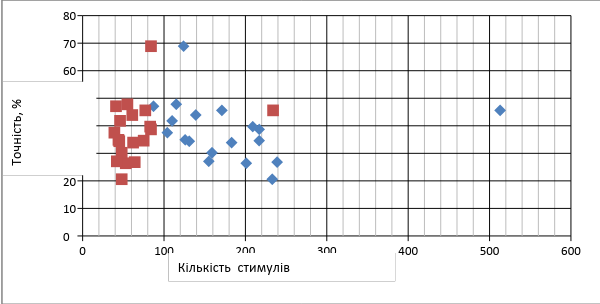
\includegraphics[width=\linewidth]{data1_irs13_total}}
	\\
	\subbottom[Розподіл за таблицею \ref{tbl:data1_irs24_total} \label{img:data1_irs24_total}]{%
		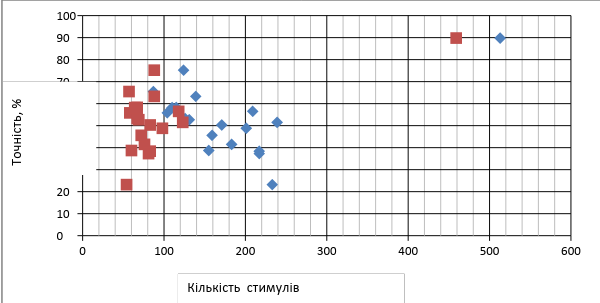
\includegraphics[width=\linewidth]{data1_irs24_total}}
	\caption{Розподіл точності розпізнання при відповідних стимулах: розпізнаних (червоні) та загальної кількості (сині) при апробації засобів формалізації голосової інформації в системах диспетчерського контролю за рухом автотранспорту для даних}
	\label{img:data1_irs}
\end{figure}

Була висунута гіпотеза про недостатню кількість вхідних даних. Були зібрані додаткові голосові дані для одного контексту: 1 пристрій, 1 диктор (чоловік), \todo{?} варіантів стимулів, 3 реакції у контексті, 938 зразків (табл. \ref{tbl:data2_irs13_total}, \ref{tbl:data2_irs24_total}).

Моделювання рефлекторними системами для одного контексту з великою вибіркою даних дало менше 70\% точності. Моделювання нейронною мережею дало більше 90\%.

\begin{longtable}[c]{ | >{\centering\arraybackslash}m{3.3cm} | >{\centering\arraybackslash}m{3.3cm} | >{\centering\arraybackslash}m{3.3cm} | >{\centering\arraybackslash}m{3.3cm} | }
	\longtableheader%
	{Відсоток розпізнавання за контекстами другого набору даних використовуючи ІРС з послідовностями розміром 1--3}%
	{tbl:data2_irs13_total}%
	{№ Контексту & Точність розпізнання & Кількість розпізнаних стимулів & Загальна кількість стимулів в контексті}	
	
	Тестовий контекст & 25.8 & 239 & 925 \\
\end{longtable}%

\begin{longtable}[c]{ | >{\centering\arraybackslash}m{3.3cm} | >{\centering\arraybackslash}m{3.3cm} | >{\centering\arraybackslash}m{3.3cm} | >{\centering\arraybackslash}m{3.3cm} | }
	\longtableheader%
	{Відсоток розпізнавання за контекстами другого набору даних використовуючи ІРС з послідовностями розміром 2--4}%
	{tbl:data2_irs24_total}%
	{№ Контексту & Точність розпізнання & Кількість розпізнаних стимулів & Загальна кількість стимулів в контексті}
	
	Тестовий контекст & 59.8 & 553 & 925 \\
\end{longtable}%

Далі, також, була висунута наступна гіпотеза про недостатню якість вхідних голосових даних: втраті деяких діапазонів частот при записі на мобільному пристрої та погано вплинуло на роботу фонемного стенографа. Були зібрані додаткові голосові дані на ПК за допомогою якісного USB мікрофона і з використанням функції запису додатку фонемного стенографа, як і в оригінальній роботі: 1 пристрій, 1 диктор (чоловік), \todo{?} варіантів стимулів, 64 реакції, 3200 зразків. Результати досліджень при апробації засобів формалізації голосової інформації в системах диспетчерського контролю за рухом автотранспорту за пристроями приведені в табл. \ref{tbl:data3_irs13_total}, \ref{tbl:data3_irs24_total}.

\begin{longtable}[c]{ | >{\centering\arraybackslash}m{3.3cm} | >{\centering\arraybackslash}m{3.3cm} | >{\centering\arraybackslash}m{3.3cm} | >{\centering\arraybackslash}m{3.3cm} | }
	\longtableheader%
	{Відсоток розпізнавання за контекстами третього набору даних використовуючи ІРС}%
	{tbl:data3_irs13_total}%
	{№ Контексту & Точність розпізнання & Кількість розпізнаних стимулів & Загальна кількість стимулів в контекст}
	
	1 & 80 & 80 & 100 \\
	\hline
	3 & 57.7 & 202 & 350 \\
	\hline
	4 & 76 & 152 & 200 \\
	\hline
	5 & 66 & 198 & 300 \\
	\hline
	6 & 70 & 140 & 200 \\
	\hline
	7 & 57.2 & 286 & 500 \\
	\hline
	8 & 66 & 198 & 300 \\
	\hline
	9 & 73.2 & 183 & 250 \\
	\hline
	10 & 72 & 180 & 250 \\
	\hline
	11 & 68 & 170 & 250 \\
	\hline
	12 & 53.1 & 239 & 450 \\
	\hline
	13 & 74.7 & 112 & 150 \\
	\hline
	14 & 52.3 & 157 & 300 \\
	\hline
	15 & 63.3 & 190 & 300 \\
	\hline
	16 & 65.6 & 164 & 250 \\
	\hline
	17 & 41.7 & 146 & 350 \\
	\hline
	18 & 64 & 160 & 250 \\
	\hline
	19 & 70.5 & 141 & 200 \\
	\hline
	По всій вибірці & 31 & 991 & 3200 \\
	\hline
	Тестовий контекст & 79.3 & 119 & 150 \\
\end{longtable}%

\begin{longtable}[c]{ | >{\centering\arraybackslash}m{3.3cm} | >{\centering\arraybackslash}m{3.3cm} | >{\centering\arraybackslash}m{3.3cm} | >{\centering\arraybackslash}m{3.3cm} | }
	\longtableheader%
	{Відсоток розпізнавання за контекстами третього набору даних використовуючи ІРС з послідовностями розміром 2--4}%
	{tbl:data3_irs24_total}%
	{№ Контексту & Точність розпізнання & Кількість розпізнаних стимулів & Загальна кількість стимулів в контекст}
	
	1 & 92.4 & 85 & 100 \\
	\hline
	3 & 86.6 & 303 & 350 \\
	\hline
	4 & 87 & 174 & 200 \\
	\hline
	5 & 83 & 249 & 300 \\
	\hline
	6 & 83.5 & 167 & 200 \\
	\hline
	7 & 77.4 & 387 & 500 \\
	\hline
	8 & 85.7 & 257 & 300 \\
	\hline
	9 & 88.8 & 221 & 250 \\
	\hline
	10 & 86.4 & 216 & 250 \\
	\hline
	11 & 82.4 & 206 & 250 \\
	\hline
	12 & 75.1 & 338 & 450 \\
	\hline
	13 & 84.1 & 122 & 150 \\
	\hline
	14 & 73 & 219 & 300 \\
	\hline
	15 & 78 & 234 & 300 \\
	\hline
	16 & 84 & 210 & 250 \\
	\hline
	17 & 64.6 & 226 & 350 \\
	\hline
	18 & 74 & 185 & 250 \\
	\hline
	19 & 82.5 & 165 & 200 \\
	\hline
	По всій вибірці & 63.7 & 2038 & 3200 \\
	\hline
	Тестовий контекст & 89.3 & 134 & 150 \\
\end{longtable}%

Розподіл точності розпізнання при відповідних стимулах: розпізнаних (червоні) та загальної кількості (сині) при апробації засобів формалізації голосової інформації в системах диспетчерського контролю за рухом автотранспорту для даних табл. \ref{tbl:data3_irs13_total}, \ref{tbl:data3_irs24_total} приведено на рис. \ref{img:data3_irs}.

\begin{figure}
	\centering
	\subbottom[Розподіл за таблицею \ref{tbl:data3_irs13_total} \label{img:data3_irs13_total}]{%
		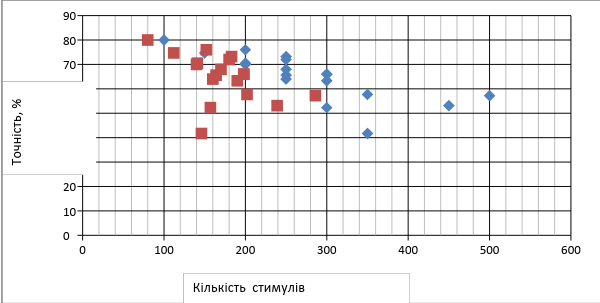
\includegraphics[width=\linewidth]{data3_irs13_total}}
	\\
	\subbottom[Розподіл за таблицею \ref{tbl:data3_irs24_total} \label{img:data3_irs24_total}]{%
		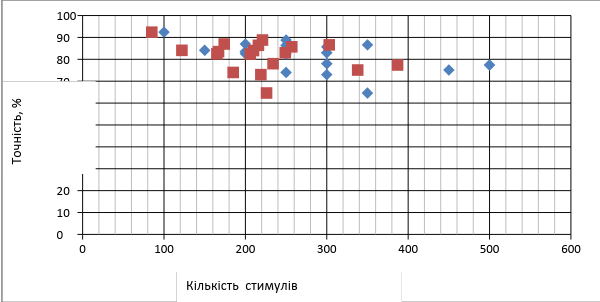
\includegraphics[width=\linewidth]{data3_irs24_total}}
	\caption{Розподіл точності розпізнання при відповідних стимулах: розпізнаних (червоні) та загальної кількості (сині) при апробації засобів формалізації голосової інформації в системах диспетчерського контролю за рухом автотранспорту для даних}
	\label{img:data3_irs}
\end{figure}

Порівнюючи дані розподілів, що приведені на рис. \ref{img:data1_irs} та \ref{img:data3_irs} можемо твердити про те, що з підвищенням загальної кількості стимулів відбувається зріст розпізнаних стимулів, що призводить до збільшення точності розпізнання при апробації засобів формалізації голосової інформації в системах диспетчерського контролю за рухом автотранспорту.

Моделювання рефлекторними системами при апробації засобів формалізації голосової інформації в системах диспетчерського контролю за рухом автотранспорту у цілому так і не дало результату, а для одного контексту дало близько 80\% точності (табл. \ref{tbl:data3_irs13_total}, \ref{tbl:data3_irs24_total} та рис. \ref{img:data3_irs}). Моделювання нейронною мережею майже не дало приросту в розпізнаванні, що свідчить про ефективність навчання згорткових фільтрів порівняно з попередньою обробкою.

\section*{Висновки до розділу 4}
\addcontentsline{toc}{section}{Висновки до розділу 4}

У розділі досліджені засоби формалізації голосової інформації в системах диспетчерського контролю за рухом автотранспорту.

При цьому, розглянуті особливості використання розроблених засобів формалізації голосової інформації в системах диспетчерського контролю за рухом автотранспорту показали, що для водія автомобілю, який буде здійснювати доставку продукції в процесі дистрибуції і вперше зіштовхнеться з засобом формалізації голосової інформації, що діє в рамках системи диспетчерського контролю за рухом автотранспорту, буде необхідно навчити систему розпізнавати його особистий голос з відповідним контекстом. Розроблений засіб формалізації голосової інформації дозволяє водію не відволікатись від управління автомобілем і слідкувати за дорожніми умовами та обстановкою, що дає змогу прискорити доставку продукції в процесі дистрибуції, а також забезпечити і підвищити рівень безпеки.

Проведена апробація засобів формалізації голосової інформації в системах диспетчерського контролю за рухом автотранспорту відбувалась за допомогою 4 пристроїв, 23 дикторів (11 жінок, 12 чоловіків), 94 варіантами стимулів (64 на основні реакції), 3046 зразків, додатково було прийнято 23 варіанти стимулів та 465 голосових зразків для реакції розпізнавання часу.

На декількох етапах досліджень рефлекторними системами як у цілому так і за контекстами не дало результатів. Точність під час навчання ЗНМ, на навчальних даних досягала 100\% і, відповідно, свідчило про перенавчання системи. Тому, далі, висунуто гіпотезу про недостатню кількість вхідних даних. У результаті було зібрано додаткові голосові дані для одного контексту: 1 пристрій, 1 диктор (чоловік), 925 варіантів стимулів, 3 реакції у контексті, 938 зразків, що призвело при моделюванні рефлекторними системами для одного контексту з великою вибіркою даних – до отримання точності не більше 70\%, а при ЗНМ – отримано точність більше 90\%.

Дослідження на цьому не були припинені, а, знову, була висунута наступна гіпотеза про недостатню якість вхідних голосових даних: втраті деяких діапазонів частот при записі на мобільному пристрої та погано вплинуло на роботу фонемного стенографа. Вирішено було зібрати додаткові голосові дані на ПК за допомогою якісного USB мікрофона і з використанням функції запису додатку фонемного стенографа, як і в оригінальній роботі: 1 пристрій, 1 диктор (чоловік), 350 варіантів стимулів, 64 реакції, 3200 зразків. Результати досліджень при апробації засобів формалізації голосової інформації в системах диспетчерського контролю за рухом автотранспорту показали те, що з підвищенням загальної кількості стимулів відбувається зріст розпізнаних стимулів, що призводить до збільшення точності розпізнання.

Підсумовуючи результати досліджень, можна стверджувати, що моделювання рефлекторними системами при апробації засобів формалізації голосової інформації в системах диспетчерського контролю за рухом автотранспорту у цілому так і не дало результату, а для одного контексту дало близько 80\% точності. Моделювання ЗНМ майже не дало приросту в розпізнаванні, що свідчить про ефективність навчання згорткових фільтрів порівняно з попередньою обробкою. Можна припустити що таке навчання не тільки знижує вимоги до вхідного звукового сигналу, а й у випадку низької якості звукових даних здатне відновити дані частково втрачені на етапі фонемного стенографа.
           % Глава 4
\chapter*{Висновки}						% Заголовок
\addcontentsline{toc}{chapter}{Висновки}	% Добавляем его в оглавление

%% Согласно ГОСТ Р 7.0.11-2011:
%% 5.3.3 В заключении диссертации излагают итоги выполненного исследования, рекомендации, перспективы дальнейшей разработки темы.
%% 9.2.3 В заключении автореферата диссертации излагают итоги данного исследования, рекомендации и перспективы дальнейшей разработки темы.
%% Поэтому имеет смысл сделать эту часть общей и загрузить из одного файла в автореферат и в диссертацию:

Основные результаты работы заключаются в следующем.
%%% Согласно ГОСТ Р 7.0.11-2011:
%% 5.3.3 В заключении диссертации излагают итоги выполненного исследования, рекомендации, перспективы дальнейшей разработки темы.
%% 9.2.3 В заключении автореферата диссертации излагают итоги данного исследования, рекомендации и перспективы дальнейшей разработки темы.
У дисертаційній роботі вирішено актуальне наукове завдання розробки моделей і методів формалізації голосової інформації в системах диспетчерського контролю за рухом автотранспорту. Загалом можна зробити наступні висновки.

1. Дослідження теоретико-методологічних засад формалізації голосової інформації в системах дистрибуції показало, що значну роль в їх управлінні відіграють процеси голосової взаємодії особливо стосовно своєчасного коригування планових маршрутів руху автотранспорту. Розроблення моделі голосової взаємодії без блоку переведення звуку голосу в текст може принципово покращити автоматизацію голосової взаємодії в системах контролю дистрибуції.

%Сучасний етап автоматизації голосового управління в організаційно-технічних системах характеризується проблемою вчасного корегування маршруту, що призводить до витрат часу на комунікацію. Встановлено, що процес автоматизації управління в системах дистрибуції повинен включати етап моніторингу руху автомобілів у режимі реального часу, а існуючі системи є занадто простими, що не зможуть справитись з задачами дистрибуції для використання в управлінні транспортними доставками.

2. Розроблена система автоматичного розрахунку планових маршрутів та практика її використання забезпечили накопичення параметрів непередбачуваних ситуацій в процесі доставки, що впливають на створення сценаріїв голосової взаємодії, які представляються у вигляді орієнтованого графу та контекстів взаємодії. 
Принципи побудови рефлекторних систем на основі теорії несилової взаємодії адаптовано для формалізації голосової інформації в системах диспетчерського контролю за рухом автотранспорту.

%Проаналізовані сучасні інформаційні системи обробки та формалізації голосової інформації показали існування достатньої кількості таких методів. Встановлено, що недоліком традиційних систем розпізнання мови є те, що вони не забезпечують автоматизацію голосової взаємодії в задачах управління дистрибуцією, оскільки це потребує додаткових технічних та телекомунікаційних засобів. Орієнтуючись на новітні підходи до автоматизації голосової взаємодії встановлено необхідність застосування теорії несилової взаємодії з рефлекторною системою голосового управління, що включає аналіз інформаційної складової та виконання відомої реакції відповідним обʼєктом.

3. Розроблено модель голосової взаємодії субʼєктів дистрибуції в системах диспетчерського контролю за рухом автотранспорту, яка представлена у вигляді повного графу сценаріїв усіх етапів дистрибуції «склад – дорога – точка доставки». Виділено перелік унікальних контекстів голосової взаємодії, формалізація голосової інформації в яких може відбуватися незалежно, що дозволяє знизити кількість реакцій для автоматизованого розпізнання.

%Під час дослідження процесу автоматизації руху автотранспорту в дистрибуції та розгляд принципів побудови рефлекторної системи голосової взаємодії встановлено, що найбільш перспективним напрямом, який дає змогу запропонувати нове принципове рішення і побудувати рефлекторну модель голосової взаємодії в задачах управління дистрибуцією є застосування моделей логічних сценаріїв взаємодії у процесах дистрибуції, які мають враховувати параметри основних причин невідповідності реальної ситуації запланованому маршруту. Тому набула подальшого розвитку модель на трьох етапах дистрибуції, проблемні моменти в якій вирішуються із залученням диспетчера для вибору найкращої стратегії і мінімізації втрат, яка є основою для побудови дерева сценаріїв голосової взаємодії для кожного з субʼєктів (диспетчера та водія). Дерево сценаріїв запропоновано будувати у вигляді орієнтовного графу і використовувати такі сутності як: Контекст або Стан, Стимул або Подія, Реакція системи відповідно до стимулу. Крім того, для побудови рефлекторної системи голосової взаємодії встановлено закономірності застосування теорії несилової взаємодії як основи інтелектуальних рефлекторних систем та теоретично запропоновано використовувати рефлекторний метод в системі голосової взаємодії диспетчерського контролю за рухом автотранспорту.

4. Створено метод формалізації голосової інформації в системах підтримки диспетчеризації автотранспорту з використанням інтелектуальних рефлекторних систем, що дозволяє автоматизувати голосову взаємодію субʼєктів дистрибуції з уникненням переводу звукової інформації в лексичний текст за рахунок використання двох основних модулів (автоматичного фонетичного стенографа і ядра рефлекторної системи голосового управління). Для реалізації ядерного компонента запропоновано дуальну систему класифікації голосових команд, яка може використовувати метод інтелектуальних рефлекторних систем або метод згорткових нейронних мереж.

%Під час розгляду методів формалізації голосової інформації в системах диспетчерського контролю за рухом автотранспорту вперше отримано модель голосової взаємодії водія в системах диспетчерського контролю за рухом автотранспорту, яка представлена у вигляді дерева сценаріїв усіх етапів дистрибуції «склад – дорога – точка доставки» та визначено перелік контекстів та можливих реакцій на них.

%В системі формалізації голосової інформації в моделі голосової взаємодії водія при диспетчерському контролі за рухом автотранспорту удосконалено процес формалізації голосової інформації, що складається з двох основних модулів: автоматичного фонетичного стенографа і ядра рефлекторної системи голосового управління, поточна реалізація яких визначає умови їх використання в моделі голосової взаємодії;

%Для формалізації голосової інформації вперше запропоновано використовувати згорткові нейронні мережі. У даному випадку система формалізації голосової інформації в моделі голосової взаємодії водія при диспетчерському контролі за рухом автотранспорту містить фонемний стенограф та згорткову нейронну мережу, яка працює з фонемами.

%Крім того, отримали подальший розвиток інтелектуальні рефлекторні системи, що призначені для формалізації голосової інформації, що представлені у термінах згорткових нейронних мереж та, які дають можливість отримати оптимальні значення параметрів шляхом навчання методом зворотного розповсюдження помилки.

5. Оцінка ефективності дуальної системи формалізації голосової інформації проведена експериментальним шляхом у три етапи: на першому етапі первинного моделювання виявлено необхідність збільшення кількості вхідних даних; на другому перевірено гіпотезу недостатності кількості вхідних даних; на третьому --- гіпотезу недостатньої якості звукового сигналу. Прийнятний для практичного використання рівень точності в моделі, побудованій методом згорткових нейронних мереж досягнуто на другому етапі моделювання, а в моделі, побудованій методом інтелектуальних рефлекторних систем --- на третьому.

Аналіз результатів моделювання показав що застосування дерева сценаріїв та розбиття повного набору команд на контексти є доцільним, оскільки значення точності без використання контекстів є найменшими для обох методів класифікації. Порівняння результатів моделювання для різних методів класифікації показало що обидва методи можуть бути використані на практиці, причому навчання моделі при використанні методу інтелектуальних рефлекторних систем набагато швидше ніж для згорткових нейронних мереж, але фактичне розпізнавання на навченій системі відбувається швидше з використанням згорткових нейронних мереж. Точність моделювання також вища при використанні згорткових нейронних мереж.

6. Впровадження протягом року у трьох дистрибуційних компаніях підтвердило ефективність розробленої інформаційної технології формалізації голосової інформації: система підтримки диспетчеризації автотранспорту підвищує загальну ефективність процесу доставки за рахунок скорочення кількості необхідних транспортних засобів та підвищення кількості точок які можуть бути обслуговуванні одним транспортним засобом; запровадження голосового інтерфейсу може підвищити відсоток уникнення чи виправлення водіями інцидентів і відхилень від планового маршруту.

%У результаті проведених експериментальних досліджень формалізації голосової інформації, отриманої від водіїв, набув подальшого розвитку процес моделювання рефлекторними системами, в якому отримано нові дані під час апробації засобів формалізації голосової інформації в системах диспетчерського контролю за рухом автотранспорту, які призначені для оптимізації диспетчерського контролю за рухом автотранспорту при виконанні процесів дистрибуції. Крім того, результати досліджень при апробації засобів формалізації голосової інформації в системах диспетчерського контролю за рухом автотранспорту показали те, що з підвищенням загальної кількості стимулів відбувається зріст розпізнаних стимулів, що призводить до збільшення точності розпізнання.

%И какая-нибудь заключающая фраза.
      % Заключение
%%\include{acronyms}        % Список сокращений и условных обозначений
%%\include{dictionary}      % Словарь терминов
\clearpage                                  % В том числе гарантирует, что список литературы в оглавлении будет с правильным номером страницы
\label{references}
%\hypersetup{ urlcolor=black }               % Ссылки делаем чёрными
%\providecommand*{\BibDash}{}                % В стилях ugost2008 отключаем использование тире как разделителя 
\urlstyle{rm}                               % ссылки URL обычным шрифтом
\ifdefmacro{\microtypesetup}{\microtypesetup{protrusion=false}}{} % не рекомендуется применять пакет микротипографики к автоматически генерируемому списку литературы
\insertbibliofull                           % Подключаем Bib-базы
\ifdefmacro{\microtypesetup}{\microtypesetup{protrusion=true}}{}
\urlstyle{tt}                               % возвращаем установки шрифта ссылок URL
%\hypersetup{ urlcolor={urlcolor} }          % Восстанавливаем цвет ссылок
\label{references_end}      % Список литературы
%\include{lists}           % Списки таблиц и изображений (иллюстративный материал)

%%% Настройки для приложений
\appendix
% Оформление заголовков приложений ближе к ГОСТ:
\setlength{\midchapskip}{20pt}
\renewcommand*{\afterchapternum}{\par\nobreak\vskip \midchapskip}
\renewcommand\thechapter{\Asbuk{chapter}} % Чтобы приложения русскими буквами нумеровались

%\chapter{Оригінальні коментарі до статусу доставки, що використувуються в різних компаніях} \label{AppendixA}

\begin{mytable*}{ | p{16cm} | }%
	{Оригінальні коментарі до статусу доставки що використувуются в різних компаніях}%
	{\label{tbl:original_comments}}%
	{\textbf{Коментар до статусу доставки}}
	
	Відмова клієнта прийняти товар \\
	\nopagebreak\quad Відмова клієнта прийняти, замінити чи повернути обладнання \\
	\nopagebreak\quad Не приймає продукцію, експедитор доставив товар на зазначену адресу вчасно \\
	\hline
	Відсутність клієнта \\
	\nopagebreak\quad Клієнт забув про доставку \\
	\nopagebreak\quad Особисті причини (пішов у лікарню, пагане самопочуття, викликали на роботу, пішов на навчання, інше) \\
	\nopagebreak\quad Некоректний номер телефону для звʼязку, недодзвон \\
	\nopagebreak\quad Немає на місці, немає звʼязку \\
	\hline
	Немає грошей \\
	\nopagebreak\quad Відсутність у клієнта коштів, експедитор доставив товар на зазначену адресу вчасно \\
	\hline
	Немає тари \\
	\nopagebreak\quad Відсутність у клієнта тари, експедитор доставив товар на зазначену адресу вчасно \\
	\hline
	Інше \\
	\nopagebreak\quad Експедитор застряг у ліфті \\
	\nopagebreak\quad За станом здоровʼя експедитора \\
	\nopagebreak\quad Заблокований вʼїзд/виїзд автомобіля доставки \\
	\nopagebreak\quad Затримка у попереднього клієнта \\
	\nopagebreak\quad Не працює ліфт, клієнт проживає вище 9-го поверху \\
	\nopagebreak\quad Немає можливості  відмінити замовлення, заявка опрацьована Логістом \\
	\nopagebreak\quad Немає підʼїзду до будинку (будів., дорожні роботи, припаркований транспорт і т.д.) обїхати неможливо \\
	\nopagebreak\quad Непередбачувані обставини (відсутність світла, інтернету тощо) \\
	\nopagebreak\quad Транспортний затор на маршруті \\
	\nopagebreak\quad У клієнта відсутні копії документів \\
	\nopagebreak\quad У клієнта немає печатки \\
	\nopagebreak\quad Транспортний засіб попав у ДТП \\
	\hline
	Погодні умови \\
	\nopagebreak\quad Складні погодні умови (автотранспорт фізично не може доїхати до місця доставки) \\
	\hline
	Невчасна доставка \\
	\nopagebreak\quad Невчасний (запізнення/достроковий) приїзд на точку доставку, клієнт не має змоги прийняти товар \\
	\hline
	Неякісна експедиція \\
	\nopagebreak\quad Відсутність перепускних документів (паспорт, тощо) у експедитора \\
	\nopagebreak\quad Пізно виїхав \\
	\nopagebreak\quad Експедитор не відразу повідомив диспетчера про недовози та їх причини (довідалися в кінці дня) \\
	\nopagebreak\quad Експедитор недотримувався маршруту руху \\
	\nopagebreak\quad Забруднена продукція (пил, бруд, стійкий сторонній запах) \\
	\nopagebreak\quad Завантажений "пересорт" товару \\
	\nopagebreak\quad Не завантажено відповідна до накладних кількість товару на складі \\
	\nopagebreak\quad Немає  накладної \\
	\nopagebreak\quad Недостатня кількість персоналу експедиції \\
	\nopagebreak\quad Пошкодження/втрата бутлів або додаткової продукції, що призначені для клієнта \\
	\hline
	Неякісна логістика \\
	\nopagebreak\quad Багато ранкових замовлень \\
	\nopagebreak\quad Виконання точок іншого маршруту \\
	\nopagebreak\quad Відсутність необхідної кількості транспорту для здійснення доставки \\
	\nopagebreak\quad Відсутність товару на складі \\
	\nopagebreak\quad Затримка завантаження товару на складі за умови вчасної подачі автомобіля \\
	\nopagebreak\quad Неправильне присвоєння сектору/координат \\
	\nopagebreak\quad Неправильно розрахований тонаж та/або обєм продукції (товар не вміщується в авто) \\
	\nopagebreak\quad Похибка при складанні маршруту (адреса точки доставки випадає з логіки загального маршруту) \\
	\hline
	Проблема з транспортом \\
	\nopagebreak\quad Невиїзд запланованого автотранспорту на маршрут \\
	\nopagebreak\quad Поломка ТЗ на маршруті \\
	\hline
	Неправильне замовлення \\
	\nopagebreak\quad Відсутня тара (оператор не попередив), експедитор доставив товар на зазначену в заявці адресу вчасно \\
	\nopagebreak\quad Задвоєне замовлення, половина повертається, експедитор доставив товар на адресу в заявці вчасно \\
	\nopagebreak\quad Клієнт не робив замовлення \\
	\nopagebreak\quad Не вказаний обід, експедитор не може чекати \\
	\nopagebreak\quad Невірно встановлено дату або час, експедитор доставив товар на зазначену в заявці адресу вчасно \\
	\nopagebreak\quad Неправильна адреса, або недостатньо інформації для доставки замовлення \\
	\nopagebreak\quad У документах зазначено товар, який клієнт не замовляв, експедитор доставив згідно накладної вчасно \\
	\hline
	Не встигли вчасно доїхати \\
	\hline
	не знайшли адресу \\
	\hline
	дуже щільний графік \\
	\hline
	запізно виїхали з бази \\
	\hline
	надзвичайні пробки на дорозі \\
	\hline
	надзвичайні погодні умови  \\
	\hline
	дорога до клієнта заблокована \\
	\hline
	технічна несправність автомобіля  \\
	\hline
	аварія автомобіля (ДТП) \\
	\hline
	Клієнт відсутній на місці \\
	\hline
	клієнт не зміг бути вчасно \\
	\hline
	зачинено, телефони не відповідають \\
	\hline
	короткий робочий день, вихідний \\
	\hline
	клієнт зʼїхав з адреси \\
	\hline
	Помилка в замовленні \\
	\nopagebreak\quad не замовляли взагалі \\
	\nopagebreak\quad замовляли на інший день \\
	\nopagebreak\quad замовляли на іншу адресу \\
	\nopagebreak\quad замовляли на інший час \\
	\nopagebreak\quad замовляли інший товар \\
	\hline
	Пошкоджений або відсутній товар \\
	\nopagebreak\quad товар не завантажено  \\
	\nopagebreak\quad товар забруднений \\
	\nopagebreak\quad товар недоукомплектований \\
	\nopagebreak\quad товар не працює (внутрішня поломка) \\
	\nopagebreak\quad товар пошкоджено зовні \\
	\hline
	Скасовано клієнтом (на місці) \\
	\hline
	немає грошей, щоб оплатити замовлення \\
	\hline
	немає потрібної контактної особи \\
	\hline
	закрито доступ до приміщення кліента \\
	\hline
	відсутні бухгалтерські документи \\
	\hline
	помилки в бухгалтерських документах \\
	\hline
	клієнт змінив свої плани щодо замовлення \\
	\hline
	відсутні печатка/пасп.дані клієнта \\
	\hline
	відмовляються сплатити борг (оренду, заставу) \\
	\hline
	не згодні з взаєморозрахунками \\
	\hline
	отримувач не відомий \\
	\hline
	Адреси не існує \\
	\hline
	Невдала спроба доставки \\
	\nopagebreak\quad зміна адреси/переадресація \\
	\nopagebreak\quad за адресою не відчиняють \\
	\nopagebreak\quad не доїхав - нема дорожнього покриття \\
	\nopagebreak\quad не виконав \\
	\nopagebreak\quad з технічних причин \\
	\nopagebreak\quad отримувач переніс дату доставки \\
	\nopagebreak\quad немає грошей \\
	\nopagebreak\quad курʼєр не встигає \\
	\nopagebreak\quad відмова отримувача (утилізація) \\
	\hline
	Заявка на відмову \\
	\nopagebreak\quad брак/пошкодження товару \\
	\nopagebreak\quad невідповідність вкладень замовленню \\
	\nopagebreak\quad нічого не замовляв \\
	\nopagebreak\quad замовлення не актуальне \\
	\nopagebreak\quad немає грошей \\
	\nopagebreak\quad недійсні/некомплектні документи отримувача (кредитна доставка) \\
	\hline
	Відправлення втрачено \\
	\hline
	никого нет дома \\
	\hline
	нет денег \\
	\hline
	говорят, что не заказывали \\
	\hline
	Никого нет \\
	\hline
	Отказ \\
	\hline
	не хотят \\
	\hline
	не просили \\
	\hline
	отобрали и денег не дали \\
	\hline
	Поломка автомобиля \\
	\hline
	Нет доверенности \\
	\hline
	Не успел водитель \\
	\hline
	Нет товароведа \\
	\hline
	Точка закрыта \\
	\hline
	Нет на месте \\
	\hline
	Частичная доставка (бой,рем кулера) \\
	\hline
	Водитель \\
	\nopagebreak\quad Нарушен временной интервал \\
	\nopagebreak\quad Бой балонов \\
	\nopagebreak\quad Не смог найти \\
	\nopagebreak\quad Отмена визита водителем \\
	\hline
	Клиент \\
	\nopagebreak\quad Клиента нет дома \\
	\nopagebreak\quad Отказ клиента на месте \\
	\nopagebreak\quad Отмена визита Клиентом \\
	\nopagebreak\quad Нет тары к возврату \\
	\hline
	Офис \\
	\nopagebreak\quad Неверный адрес \\
	\nopagebreak\quad Отмена визита офисом \\
	\nopagebreak\quad Ошибка офиса  \\
	\hline
	Некорректный маршрут \\
	\hline
	Ошибка склада \\
	\hline
	Форс-мажор \\
	\nopagebreak\quad Поломка авто \\
	\nopagebreak\quad ДТП \\
	\nopagebreak\quad Не выход водителя \\
	\nopagebreak\quad Не поместилось в машину \\
	\nopagebreak\quad Не было места для парковки \\
	\nopagebreak\quad Авто не прошло по габаритам \\
	\nopagebreak\quad Перекрытие дороги \\
	\nopagebreak\quad Нет подъезда к клиенту \\
	\nopagebreak\quad Несвоевременный вызов водителя на маршрут \\
	\nopagebreak\quad Не работает лифт (Выше 5-го этажа) \\
	\hline
	Состояние здоровья водителя \\
	\hline
	Другое \\
	\hline
	Точка закрыта \\
\end{mytable*}%


\chapter{Детальні таблиці точності розпізнавання по реакціях} \label{AppendixB}

\begin{mytable*}{ | c | c | c | c | c | c | }%
	{Результати моделювання конкретних реакцій першого набору даних використовуючи ІРС з послідовностями розміром 1--3}%
	{\label{tbl:detailed_data1_irs13}}%
	{№ Контексту & № Реакції & Точність & Прецизійність & Повнота & F-міра}
	
	1 & 5 & 0.750 & 0.711 & 0.730 & 0.613 \\
\hline
1 & 6 & 0.600 & 0.625 & 0.612 & 0.387 \\
\hline
2 & 6 & 0.138 & 0.917 & 0.240 & 0.094 \\
\hline
2 & 41 & 0.979 & 0.409 & 0.577 & 0.906 \\
\hline
3 & 1 & 0.000 & 0.000 & 0.000 & 0.120 \\
\hline
3 & 32 & 0.000 & 0.000 & 0.000 & 0.097 \\
\hline
3 & 33 & 0.000 & 0.000 & 0.000 & 0.088 \\
\hline
3 & 35 & 0.000 & 0.000 & 0.000 & 0.097 \\
\hline
3 & 55 & 0.000 & 0.000 & 0.000 & 0.101 \\
\hline
3 & 56 & 0.000 & 0.000 & 0.000 & 0.111 \\
\hline
3 & 57 & 0.387 & 1.000 & 0.558 & 0.387 \\
\hline
4 & 8 & 0.500 & 0.083 & 0.143 & 0.231 \\
\hline
4 & 31 & 0.000 & 0.000 & 0.000 & 0.202 \\
\hline
4 & 58 & 0.000 & 0.000 & 0.000 & 0.212 \\
\hline
4 & 59 & 0.370 & 1.000 & 0.540 & 0.356 \\
\hline
5 & 8 & 0.000 & 0.000 & 0.000 & 0.131 \\
\hline
5 & 31 & 0.000 & 0.000 & 0.000 & 0.115 \\
\hline
5 & 60 & 0.000 & 0.000 & 0.000 & 0.115 \\
\hline
5 & 61 & 0.341 & 1.000 & 0.509 & 0.317 \\
\hline
5 & 62 & 0.000 & 0.000 & 0.000 & 0.115 \\
\hline
5 & 63 & 0.308 & 0.105 & 0.157 & 0.208 \\
\hline
6 & 8 & 0.000 & 0.000 & 0.000 & 0.115 \\
\hline
6 & 31 & 0.000 & 0.000 & 0.000 & 0.100 \\
\hline
6 & 64 & 0.396 & 0.456 & 0.424 & 0.378 \\
\hline
6 & 65 & 0.398 & 0.553 & 0.463 & 0.407 \\
\hline
7 & 2 & 0.207 & 0.980 & 0.342 & 0.210 \\
\hline
7 & 32 & 0.000 & 0.000 & 0.000 & 0.090 \\
\hline
7 & 33 & 0.000 & 0.000 & 0.000 & 0.082 \\
\hline
7 & 34 & 0.000 & 0.000 & 0.000 & 0.090 \\
\hline
7 & 35 & 0.000 & 0.000 & 0.000 & 0.090 \\
\hline
7 & 36 & 0.000 & 0.000 & 0.000 & 0.086 \\
\hline
7 & 37 & 0.000 & 0.000 & 0.000 & 0.086 \\
\hline
7 & 38 & 0.000 & 0.000 & 0.000 & 0.090 \\
\hline
7 & 39 & 0.000 & 0.000 & 0.000 & 0.090 \\
\hline
7 & 40 & 0.000 & 0.000 & 0.000 & 0.086 \\
\hline
8 & 8 & 0.000 & 0.000 & 0.000 & 0.111 \\
\hline
8 & 31 & 0.000 & 0.000 & 0.000 & 0.097 \\
\hline
8 & 51 & 0.000 & 0.000 & 0.000 & 0.088 \\
\hline
8 & 52 & 0.000 & 0.000 & 0.000 & 0.184 \\
\hline
8 & 53 & 0.750 & 0.073 & 0.133 & 0.189 \\
\hline
8 & 54 & 0.343 & 1.000 & 0.511 & 0.332 \\
\hline
9 & 8 & 0.375 & 0.125 & 0.188 & 0.183 \\
\hline
9 & 31 & 0.000 & 0.000 & 0.000 & 0.160 \\
\hline
9 & 48 & 0.347 & 1.000 & 0.515 & 0.321 \\
\hline
9 & 49 & 0.000 & 0.000 & 0.000 & 0.176 \\
\hline
9 & 50 & 0.000 & 0.000 & 0.000 & 0.160 \\
\hline
10 & 8 & 0.625 & 0.208 & 0.312 & 0.190 \\
\hline
10 & 31 & 1.000 & 0.048 & 0.091 & 0.167 \\
\hline
10 & 42 & 0.500 & 0.045 & 0.083 & 0.175 \\
\hline
10 & 43 & 0.000 & 0.000 & 0.000 & 0.167 \\
\hline
10 & 44 & 0.322 & 0.974 & 0.484 & 0.302 \\
\hline
11 & 8 & 0.000 & 0.000 & 0.000 & 0.100 \\
\hline
11 & 31 & 0.000 & 0.000 & 0.000 & 0.088 \\
\hline
11 & 45 & 0.299 & 0.562 & 0.391 & 0.372 \\
\hline
11 & 46 & 0.194 & 0.165 & 0.178 & 0.356 \\
\hline
11 & 47 & 0.000 & 0.000 & 0.000 & 0.084 \\
\hline
12 & 3 & 0.182 & 0.462 & 0.261 & 0.129 \\
\hline
12 & 7 & 0.167 & 0.167 & 0.167 & 0.119 \\
\hline
12 & 8 & 0.325 & 0.542 & 0.406 & 0.119 \\
\hline
12 & 28 & 0.257 & 0.360 & 0.300 & 0.124 \\
\hline
12 & 32 & 0.500 & 0.238 & 0.323 & 0.104 \\
\hline
12 & 33 & 0.000 & 0.000 & 0.000 & 0.095 \\
\hline
12 & 34 & 0.600 & 0.286 & 0.387 & 0.104 \\
\hline
12 & 35 & 0.200 & 0.095 & 0.129 & 0.104 \\
\hline
12 & 36 & 0.500 & 0.100 & 0.167 & 0.100 \\
\hline
13 & 4 & 0.000 & 0.000 & 0.000 & 0.275 \\
\hline
13 & 5 & 0.446 & 0.974 & 0.612 & 0.444 \\
\hline
13 & 6 & 1.000 & 0.062 & 0.118 & 0.281 \\
\hline
14 & 8 & 0.296 & 0.667 & 0.410 & 0.173 \\
\hline
14 & 9 & 0.360 & 0.391 & 0.375 & 0.165 \\
\hline
14 & 10 & 0.464 & 0.542 & 0.500 & 0.173 \\
\hline
14 & 11 & 0.769 & 0.417 & 0.541 & 0.173 \\
\hline
14 & 12 & 0.667 & 0.435 & 0.526 & 0.165 \\
\hline
14 & 31 & 0.750 & 0.143 & 0.240 & 0.151 \\
\hline
15 & 8 & 0.500 & 0.042 & 0.077 & 0.151 \\
\hline
15 & 13 & 0.500 & 0.040 & 0.074 & 0.157 \\
\hline
15 & 14 & 0.667 & 0.087 & 0.154 & 0.145 \\
\hline
15 & 15 & 0.284 & 1.000 & 0.442 & 0.264 \\
\hline
15 & 16 & 0.333 & 0.042 & 0.074 & 0.151 \\
\hline
15 & 31 & 1.000 & 0.048 & 0.091 & 0.132 \\
\hline
16 & 8 & 0.395 & 0.708 & 0.507 & 0.209 \\
\hline
16 & 17 & 0.533 & 0.348 & 0.421 & 0.200 \\
\hline
16 & 18 & 0.500 & 0.565 & 0.531 & 0.200 \\
\hline
16 & 19 & 0.519 & 0.583 & 0.549 & 0.209 \\
\hline
16 & 31 & 0.750 & 0.143 & 0.240 & 0.183 \\
\hline
17 & 8 & 0.429 & 0.625 & 0.508 & 0.155 \\
\hline
17 & 20 & 0.333 & 0.348 & 0.340 & 0.148 \\
\hline
17 & 21 & 0.167 & 0.217 & 0.189 & 0.148 \\
\hline
17 & 22 & 0.292 & 0.318 & 0.304 & 0.142 \\
\hline
17 & 23 & 0.087 & 0.095 & 0.091 & 0.135 \\
\hline
17 & 24 & 0.267 & 0.190 & 0.222 & 0.135 \\
\hline
17 & 31 & 0.250 & 0.048 & 0.080 & 0.135 \\
\hline
18 & 8 & 0.315 & 0.708 & 0.436 & 0.218 \\
\hline
18 & 25 & 0.348 & 0.348 & 0.348 & 0.209 \\
\hline
18 & 26 & 0.769 & 0.476 & 0.588 & 0.191 \\
\hline
18 & 27 & 0.643 & 0.429 & 0.514 & 0.191 \\
\hline
18 & 31 & 0.333 & 0.095 & 0.148 & 0.191 \\
\hline
19 & 8 & 0.351 & 0.833 & 0.494 & 0.276 \\
\hline
19 & 29 & 1.000 & 0.381 & 0.552 & 0.241 \\
\hline
19 & 30 & 0.533 & 0.381 & 0.444 & 0.241 \\
\hline
19 & 31 & 0.714 & 0.238 & 0.357 & 0.241 \\
\hline
\specialcell{3cm}{По всій \\ вибірці} & 1 & 0.000 & 0.000 & 0.000 & 0.013 \\
\hline
\specialcell{3cm}{По всій \\ вибірці} & 2 & 0.333 & 0.020 & 0.038 & 0.024 \\
\hline
\specialcell{3cm}{По всій \\ вибірці} & 3 & 0.000 & 0.000 & 0.000 & 0.013 \\
\hline
\specialcell{3cm}{По всій \\ вибірці} & 4 & 0.000 & 0.000 & 0.000 & 0.023 \\
\hline
\specialcell{3cm}{По всій \\ вибірці} & 5 & 0.091 & 0.237 & 0.132 & 0.037 \\
\hline
\specialcell{3cm}{По всій \\ вибірці} & 6 & 1.000 & 0.021 & 0.041 & 0.023 \\
\hline
\specialcell{3cm}{По всій \\ вибірці} & 7 & 0.000 & 0.000 & 0.000 & 0.012 \\
\hline
\specialcell{3cm}{По всій \\ вибірці} & 8 & 0.000 & 0.000 & 0.000 & 0.012 \\
\hline
\specialcell{3cm}{По всій \\ вибірці} & 9 & 0.000 & 0.000 & 0.000 & 0.011 \\
\hline
\specialcell{3cm}{По всій \\ вибірці} & 10 & 0.000 & 0.000 & 0.000 & 0.012 \\
\hline
\specialcell{3cm}{По всій \\ вибірці} & 11 & 0.000 & 0.000 & 0.000 & 0.012 \\
\hline
\specialcell{3cm}{По всій \\ вибірці} & 12 & 0.000 & 0.000 & 0.000 & 0.011 \\
\hline
\specialcell{3cm}{По всій \\ вибірці} & 13 & 0.000 & 0.000 & 0.000 & 0.012 \\
\hline
\specialcell{3cm}{По всій \\ вибірці} & 14 & 0.000 & 0.000 & 0.000 & 0.011 \\
\hline
\specialcell{3cm}{По всій \\ вибірці} & 15 & 0.000 & 0.000 & 0.000 & 0.020 \\
\hline
\specialcell{3cm}{По всій \\ вибірці} & 16 & 0.000 & 0.000 & 0.000 & 0.012 \\
\hline
\specialcell{3cm}{По всій \\ вибірці} & 17 & 0.000 & 0.000 & 0.000 & 0.011 \\
\hline
\specialcell{3cm}{По всій \\ вибірці} & 18 & 0.000 & 0.000 & 0.000 & 0.011 \\
\hline
\specialcell{3cm}{По всій \\ вибірці} & 19 & 0.000 & 0.000 & 0.000 & 0.012 \\
\hline
\specialcell{3cm}{По всій \\ вибірці} & 20 & 0.000 & 0.000 & 0.000 & 0.011 \\
\hline
\specialcell{3cm}{По всій \\ вибірці} & 21 & 0.000 & 0.000 & 0.000 & 0.011 \\
\hline
\specialcell{3cm}{По всій \\ вибірці} & 22 & 0.000 & 0.000 & 0.000 & 0.011 \\
\hline
\specialcell{3cm}{По всій \\ вибірці} & 23 & 0.000 & 0.000 & 0.000 & 0.010 \\
\hline
\specialcell{3cm}{По всій \\ вибірці} & 24 & 0.000 & 0.000 & 0.000 & 0.010 \\
\hline
\specialcell{3cm}{По всій \\ вибірці} & 25 & 0.000 & 0.000 & 0.000 & 0.011 \\
\hline
\specialcell{3cm}{По всій \\ вибірці} & 26 & 0.000 & 0.000 & 0.000 & 0.010 \\
\hline
\specialcell{3cm}{По всій \\ вибірці} & 27 & 0.000 & 0.000 & 0.000 & 0.010 \\
\hline
\specialcell{3cm}{По всій \\ вибірці} & 28 & 0.000 & 0.000 & 0.000 & 0.012 \\
\hline
\specialcell{3cm}{По всій \\ вибірці} & 29 & 0.000 & 0.000 & 0.000 & 0.010 \\
\hline
\specialcell{3cm}{По всій \\ вибірці} & 30 & 0.000 & 0.000 & 0.000 & 0.010 \\
\hline
\specialcell{3cm}{По всій \\ вибірці} & 31 & 0.000 & 0.000 & 0.000 & 0.010 \\
\hline
\specialcell{3cm}{По всій \\ вибірці} & 32 & 0.000 & 0.000 & 0.000 & 0.010 \\
\hline
\specialcell{3cm}{По всій \\ вибірці} & 33 & 0.000 & 0.000 & 0.000 & 0.009 \\
\hline
\specialcell{3cm}{По всій \\ вибірці} & 34 & 0.000 & 0.000 & 0.000 & 0.010 \\
\hline
\specialcell{3cm}{По всій \\ вибірці} & 35 & 0.000 & 0.000 & 0.000 & 0.010 \\
\hline
\specialcell{3cm}{По всій \\ вибірці} & 36 & 0.000 & 0.000 & 0.000 & 0.010 \\
\hline
\specialcell{3cm}{По всій \\ вибірці} & 37 & 0.000 & 0.000 & 0.000 & 0.010 \\
\hline
\specialcell{3cm}{По всій \\ вибірці} & 38 & 0.000 & 0.000 & 0.000 & 0.010 \\
\hline
\specialcell{3cm}{По всій \\ вибірці} & 39 & 0.000 & 0.000 & 0.000 & 0.010 \\
\hline
\specialcell{3cm}{По всій \\ вибірці} & 40 & 0.000 & 0.000 & 0.000 & 0.010 \\
\hline
\specialcell{3cm}{По всій \\ вибірці} & 42 & 0.000 & 0.000 & 0.000 & 0.011 \\
\hline
\specialcell{3cm}{По всій \\ вибірці} & 43 & 0.000 & 0.000 & 0.000 & 0.010 \\
\hline
\specialcell{3cm}{По всій \\ вибірці} & 44 & 0.000 & 0.000 & 0.000 & 0.018 \\
\hline
\specialcell{3cm}{По всій \\ вибірці} & 45 & 0.031 & 0.247 & 0.055 & 0.043 \\
\hline
\specialcell{3cm}{По всій \\ вибірці} & 46 & 0.032 & 0.141 & 0.052 & 0.041 \\
\hline
\specialcell{3cm}{По всій \\ вибірці} & 47 & 0.000 & 0.000 & 0.000 & 0.010 \\
\hline
\specialcell{3cm}{По всій \\ вибірці} & 48 & 0.000 & 0.000 & 0.000 & 0.020 \\
\hline
\specialcell{3cm}{По всій \\ вибірці} & 49 & 0.000 & 0.000 & 0.000 & 0.011 \\
\hline
\specialcell{3cm}{По всій \\ вибірці} & 50 & 0.000 & 0.000 & 0.000 & 0.010 \\
\hline
\specialcell{3cm}{По всій \\ вибірці} & 51 & 0.000 & 0.000 & 0.000 & 0.009 \\
\hline
\specialcell{3cm}{По всій \\ вибірці} & 52 & 0.000 & 0.000 & 0.000 & 0.019 \\
\hline
\specialcell{3cm}{По всій \\ вибірці} & 53 & 0.000 & 0.000 & 0.000 & 0.020 \\
\hline
\specialcell{3cm}{По всій \\ вибірці} & 54 & 0.125 & 0.056 & 0.077 & 0.035 \\
\hline
\specialcell{3cm}{По всій \\ вибірці} & 55 & 0.000 & 0.000 & 0.000 & 0.011 \\
\hline
\specialcell{3cm}{По всій \\ вибірці} & 56 & 0.000 & 0.000 & 0.000 & 0.012 \\
\hline
\specialcell{3cm}{По всій \\ вибірці} & 57 & 0.044 & 0.143 & 0.067 & 0.041 \\
\hline
\specialcell{3cm}{По всій \\ вибірці} & 58 & 0.000 & 0.000 & 0.000 & 0.011 \\
\hline
\specialcell{3cm}{По всій \\ вибірці} & 59 & 0.000 & 0.000 & 0.000 & 0.018 \\
\hline
\specialcell{3cm}{По всій \\ вибірці} & 60 & 0.000 & 0.000 & 0.000 & 0.010 \\
\hline
\specialcell{3cm}{По всій \\ вибірці} & 61 & 0.000 & 0.000 & 0.000 & 0.028 \\
\hline
\specialcell{3cm}{По всій \\ вибірці} & 62 & 0.000 & 0.000 & 0.000 & 0.010 \\
\hline
\specialcell{3cm}{По всій \\ вибірці} & 63 & 0.000 & 0.000 & 0.000 & 0.018 \\
\hline
\specialcell{3cm}{По всій \\ вибірці} & 64 & 0.067 & 0.139 & 0.091 & 0.038 \\
\hline
\specialcell{3cm}{По всій \\ вибірці} & 65 & 0.037 & 0.129 & 0.057 & 0.041 \\
\hline
\specialcell{3cm}{Тестовий \\ контекст} & 1 & 0.000 & 0.000 & 0.000 & 0.257 \\
\hline
\specialcell{3cm}{Тестовий \\ контекст} & 2 & 0.485 & 1.000 & 0.653 & 0.485 \\
\hline
\specialcell{3cm}{Тестовий \\ контекст} & 3 & 0.000 & 0.000 & 0.000 & 0.257 \\
\end{mytable*}

\begin{mytable*}{ | c | c | c | c | c | c | }%
	{Результати моделювання конкретних реакцій першого набору даних використовуючи ІРС з послідовностями розміром 2--4}%
	{\label{tbl:detailed_data1_irs24}}%
	{№ Контексту & № Реакції & Точність & Прецизійність & Повнота & F-міра}
	
	1 & 5 & 0.750 & 0.868 & 0.805 & 0.613 \\
\hline
1 & 6 & 0.759 & 0.458 & 0.571 & 0.387 \\
\hline
2 & 6 & 0.444 & 0.500 & 0.471 & 0.094 \\
\hline
2 & 41 & 0.952 & 0.935 & 0.944 & 0.906 \\
\hline
3 & 1 & 0.000 & 0.000 & 0.000 & 0.120 \\
\hline
3 & 32 & 0.000 & 0.000 & 0.000 & 0.097 \\
\hline
3 & 33 & 0.000 & 0.000 & 0.000 & 0.088 \\
\hline
3 & 35 & 0.000 & 0.000 & 0.000 & 0.097 \\
\hline
3 & 55 & 0.000 & 0.000 & 0.000 & 0.101 \\
\hline
3 & 56 & 0.000 & 0.000 & 0.000 & 0.111 \\
\hline
3 & 57 & 0.384 & 0.988 & 0.553 & 0.387 \\
\hline
4 & 8 & 0.857 & 0.500 & 0.632 & 0.231 \\
\hline
4 & 31 & 0.833 & 0.238 & 0.370 & 0.202 \\
\hline
4 & 58 & 0.800 & 0.182 & 0.296 & 0.212 \\
\hline
4 & 59 & 0.468 & 1.000 & 0.638 & 0.356 \\
\hline
5 & 8 & 0.500 & 0.042 & 0.077 & 0.131 \\
\hline
5 & 31 & 1.000 & 0.143 & 0.250 & 0.115 \\
\hline
5 & 60 & 0.000 & 0.000 & 0.000 & 0.115 \\
\hline
5 & 61 & 0.365 & 1.000 & 0.535 & 0.317 \\
\hline
5 & 62 & 0.000 & 0.000 & 0.000 & 0.115 \\
\hline
5 & 63 & 0.737 & 0.368 & 0.491 & 0.208 \\
\hline
6 & 8 & 0.000 & 0.000 & 0.000 & 0.115 \\
\hline
6 & 31 & 0.000 & 0.000 & 0.000 & 0.100 \\
\hline
6 & 64 & 0.551 & 0.684 & 0.610 & 0.378 \\
\hline
6 & 65 & 0.577 & 0.753 & 0.653 & 0.407 \\
\hline
7 & 2 & 0.216 & 0.980 & 0.354 & 0.210 \\
\hline
7 & 32 & 0.667 & 0.095 & 0.167 & 0.090 \\
\hline
7 & 33 & 0.000 & 0.000 & 0.000 & 0.082 \\
\hline
7 & 34 & 0.000 & 0.000 & 0.000 & 0.090 \\
\hline
7 & 35 & 1.000 & 0.048 & 0.091 & 0.090 \\
\hline
7 & 36 & 0.000 & 0.000 & 0.000 & 0.086 \\
\hline
7 & 37 & 1.000 & 0.100 & 0.182 & 0.086 \\
\hline
7 & 38 & 0.000 & 0.000 & 0.000 & 0.090 \\
\hline
7 & 39 & 0.000 & 0.000 & 0.000 & 0.090 \\
\hline
7 & 40 & 1.000 & 0.050 & 0.095 & 0.086 \\
\hline
8 & 8 & 0.000 & 0.000 & 0.000 & 0.111 \\
\hline
8 & 31 & 1.000 & 0.048 & 0.091 & 0.097 \\
\hline
8 & 51 & 0.000 & 0.000 & 0.000 & 0.088 \\
\hline
8 & 52 & 0.500 & 0.050 & 0.091 & 0.184 \\
\hline
8 & 53 & 0.600 & 0.146 & 0.235 & 0.189 \\
\hline
8 & 54 & 0.358 & 1.000 & 0.527 & 0.332 \\
\hline
9 & 8 & 0.722 & 0.542 & 0.619 & 0.183 \\
\hline
9 & 31 & 1.000 & 0.190 & 0.320 & 0.160 \\
\hline
9 & 48 & 0.438 & 1.000 & 0.609 & 0.321 \\
\hline
9 & 49 & 0.857 & 0.261 & 0.400 & 0.176 \\
\hline
9 & 50 & 0.667 & 0.190 & 0.296 & 0.160 \\
\hline
10 & 8 & 0.650 & 0.542 & 0.591 & 0.190 \\
\hline
10 & 31 & 1.000 & 0.190 & 0.320 & 0.167 \\
\hline
10 & 42 & 0.800 & 0.182 & 0.296 & 0.175 \\
\hline
10 & 43 & 1.000 & 0.476 & 0.645 & 0.167 \\
\hline
10 & 44 & 0.414 & 0.947 & 0.576 & 0.302 \\
\hline
11 & 8 & 0.000 & 0.000 & 0.000 & 0.100 \\
\hline
11 & 31 & 0.000 & 0.000 & 0.000 & 0.088 \\
\hline
11 & 45 & 0.496 & 0.787 & 0.609 & 0.372 \\
\hline
11 & 46 & 0.541 & 0.624 & 0.579 & 0.356 \\
\hline
11 & 47 & 0.000 & 0.000 & 0.000 & 0.084 \\
\hline
12 & 3 & 0.412 & 0.808 & 0.545 & 0.129 \\
\hline
12 & 7 & 0.235 & 0.167 & 0.195 & 0.119 \\
\hline
12 & 8 & 0.514 & 0.750 & 0.610 & 0.119 \\
\hline
12 & 28 & 0.588 & 0.800 & 0.678 & 0.124 \\
\hline
12 & 32 & 0.500 & 0.381 & 0.432 & 0.104 \\
\hline
12 & 33 & 0.500 & 0.105 & 0.174 & 0.095 \\
\hline
12 & 34 & 0.400 & 0.381 & 0.390 & 0.104 \\
\hline
12 & 35 & 0.667 & 0.476 & 0.556 & 0.104 \\
\hline
12 & 36 & 0.778 & 0.350 & 0.483 & 0.100 \\
\hline
13 & 4 & 0.533 & 0.170 & 0.258 & 0.275 \\
\hline
13 & 5 & 0.482 & 0.895 & 0.627 & 0.444 \\
\hline
13 & 6 & 0.778 & 0.146 & 0.246 & 0.281 \\
\hline
14 & 8 & 0.439 & 0.750 & 0.554 & 0.173 \\
\hline
14 & 9 & 0.550 & 0.478 & 0.512 & 0.165 \\
\hline
14 & 10 & 0.588 & 0.833 & 0.690 & 0.173 \\
\hline
14 & 11 & 0.947 & 0.750 & 0.837 & 0.173 \\
\hline
14 & 12 & 0.833 & 0.652 & 0.732 & 0.165 \\
\hline
14 & 31 & 0.857 & 0.286 & 0.429 & 0.151 \\
\hline
15 & 8 & 0.167 & 0.083 & 0.111 & 0.151 \\
\hline
15 & 13 & 0.778 & 0.280 & 0.412 & 0.157 \\
\hline
15 & 14 & 0.500 & 0.348 & 0.410 & 0.145 \\
\hline
15 & 15 & 0.418 & 0.976 & 0.586 & 0.264 \\
\hline
15 & 16 & 0.500 & 0.375 & 0.429 & 0.151 \\
\hline
15 & 31 & 1.000 & 0.238 & 0.385 & 0.132 \\
\hline
16 & 8 & 0.513 & 0.833 & 0.635 & 0.209 \\
\hline
16 & 17 & 0.833 & 0.217 & 0.345 & 0.200 \\
\hline
16 & 18 & 0.667 & 0.696 & 0.681 & 0.200 \\
\hline
16 & 19 & 0.514 & 0.792 & 0.623 & 0.209 \\
\hline
16 & 31 & 0.778 & 0.333 & 0.467 & 0.183 \\
\hline
17 & 8 & 0.594 & 0.792 & 0.679 & 0.155 \\
\hline
17 & 20 & 0.458 & 0.478 & 0.468 & 0.148 \\
\hline
17 & 21 & 0.281 & 0.391 & 0.327 & 0.148 \\
\hline
17 & 22 & 0.214 & 0.273 & 0.240 & 0.142 \\
\hline
17 & 23 & 0.095 & 0.095 & 0.095 & 0.135 \\
\hline
17 & 24 & 0.667 & 0.476 & 0.556 & 0.135 \\
\hline
17 & 31 & 1.000 & 0.143 & 0.250 & 0.135 \\
\hline
18 & 8 & 0.388 & 0.792 & 0.521 & 0.218 \\
\hline
18 & 25 & 0.684 & 0.565 & 0.619 & 0.209 \\
\hline
18 & 26 & 0.750 & 0.714 & 0.732 & 0.191 \\
\hline
18 & 27 & 0.786 & 0.524 & 0.629 & 0.191 \\
\hline
18 & 31 & 0.750 & 0.286 & 0.414 & 0.191 \\
\hline
19 & 8 & 0.543 & 0.792 & 0.644 & 0.276 \\
\hline
19 & 29 & 0.941 & 0.762 & 0.842 & 0.241 \\
\hline
19 & 30 & 0.571 & 0.762 & 0.653 & 0.241 \\
\hline
19 & 31 & 0.857 & 0.286 & 0.429 & 0.241 \\
\hline
\specialcell{3cm}{По всій \\ вибірці} & 1 & 0.000 & 0.000 & 0.000 & 0.013 \\
\hline
\specialcell{3cm}{По всій \\ вибірці} & 2 & 0.600 & 0.061 & 0.111 & 0.024 \\
\hline
\specialcell{3cm}{По всій \\ вибірці} & 3 & 0.000 & 0.000 & 0.000 & 0.013 \\
\hline
\specialcell{3cm}{По всій \\ вибірці} & 4 & 0.000 & 0.000 & 0.000 & 0.023 \\
\hline
\specialcell{3cm}{По всій \\ вибірці} & 5 & 0.233 & 0.355 & 0.281 & 0.037 \\
\hline
\specialcell{3cm}{По всій \\ вибірці} & 6 & 1.000 & 0.021 & 0.041 & 0.023 \\
\hline
\specialcell{3cm}{По всій \\ вибірці} & 7 & 0.000 & 0.000 & 0.000 & 0.012 \\
\hline
\specialcell{3cm}{По всій \\ вибірці} & 8 & 0.000 & 0.000 & 0.000 & 0.012 \\
\hline
\specialcell{3cm}{По всій \\ вибірці} & 9 & 0.000 & 0.000 & 0.000 & 0.011 \\
\hline
\specialcell{3cm}{По всій \\ вибірці} & 10 & 0.000 & 0.000 & 0.000 & 0.012 \\
\hline
\specialcell{3cm}{По всій \\ вибірці} & 11 & 0.000 & 0.000 & 0.000 & 0.012 \\
\hline
\specialcell{3cm}{По всій \\ вибірці} & 12 & 0.000 & 0.000 & 0.000 & 0.011 \\
\hline
\specialcell{3cm}{По всій \\ вибірці} & 13 & 0.000 & 0.000 & 0.000 & 0.012 \\
\hline
\specialcell{3cm}{По всій \\ вибірці} & 14 & 0.000 & 0.000 & 0.000 & 0.011 \\
\hline
\specialcell{3cm}{По всій \\ вибірці} & 15 & 0.000 & 0.000 & 0.000 & 0.020 \\
\hline
\specialcell{3cm}{По всій \\ вибірці} & 16 & 0.000 & 0.000 & 0.000 & 0.012 \\
\hline
\specialcell{3cm}{По всій \\ вибірці} & 17 & 0.000 & 0.000 & 0.000 & 0.011 \\
\hline
\specialcell{3cm}{По всій \\ вибірці} & 18 & 0.000 & 0.000 & 0.000 & 0.011 \\
\hline
\specialcell{3cm}{По всій \\ вибірці} & 19 & 0.000 & 0.000 & 0.000 & 0.012 \\
\hline
\specialcell{3cm}{По всій \\ вибірці} & 20 & 0.000 & 0.000 & 0.000 & 0.011 \\
\hline
\specialcell{3cm}{По всій \\ вибірці} & 21 & 0.000 & 0.000 & 0.000 & 0.011 \\
\hline
\specialcell{3cm}{По всій \\ вибірці} & 22 & 0.000 & 0.000 & 0.000 & 0.011 \\
\hline
\specialcell{3cm}{По всій \\ вибірці} & 23 & 0.000 & 0.000 & 0.000 & 0.010 \\
\hline
\specialcell{3cm}{По всій \\ вибірці} & 24 & 0.000 & 0.000 & 0.000 & 0.010 \\
\hline
\specialcell{3cm}{По всій \\ вибірці} & 25 & 0.000 & 0.000 & 0.000 & 0.011 \\
\hline
\specialcell{3cm}{По всій \\ вибірці} & 26 & 0.000 & 0.000 & 0.000 & 0.010 \\
\hline
\specialcell{3cm}{По всій \\ вибірці} & 27 & 0.000 & 0.000 & 0.000 & 0.010 \\
\hline
\specialcell{3cm}{По всій \\ вибірці} & 28 & 0.000 & 0.000 & 0.000 & 0.012 \\
\hline
\specialcell{3cm}{По всій \\ вибірці} & 29 & 0.000 & 0.000 & 0.000 & 0.010 \\
\hline
\specialcell{3cm}{По всій \\ вибірці} & 30 & 0.000 & 0.000 & 0.000 & 0.010 \\
\hline
\specialcell{3cm}{По всій \\ вибірці} & 31 & 0.000 & 0.000 & 0.000 & 0.010 \\
\hline
\specialcell{3cm}{По всій \\ вибірці} & 32 & 0.000 & 0.000 & 0.000 & 0.010 \\
\hline
\specialcell{3cm}{По всій \\ вибірці} & 33 & 0.000 & 0.000 & 0.000 & 0.009 \\
\hline
\specialcell{3cm}{По всій \\ вибірці} & 34 & 0.000 & 0.000 & 0.000 & 0.010 \\
\hline
\specialcell{3cm}{По всій \\ вибірці} & 35 & 0.000 & 0.000 & 0.000 & 0.010 \\
\hline
\specialcell{3cm}{По всій \\ вибірці} & 36 & 0.000 & 0.000 & 0.000 & 0.010 \\
\hline
\specialcell{3cm}{По всій \\ вибірці} & 37 & 0.000 & 0.000 & 0.000 & 0.010 \\
\hline
\specialcell{3cm}{По всій \\ вибірці} & 38 & 0.000 & 0.000 & 0.000 & 0.010 \\
\hline
\specialcell{3cm}{По всій \\ вибірці} & 39 & 0.000 & 0.000 & 0.000 & 0.010 \\
\hline
\specialcell{3cm}{По всій \\ вибірці} & 40 & 0.000 & 0.000 & 0.000 & 0.010 \\
\hline
\specialcell{3cm}{По всій \\ вибірці} & 42 & 0.000 & 0.000 & 0.000 & 0.011 \\
\hline
\specialcell{3cm}{По всій \\ вибірці} & 43 & 0.000 & 0.000 & 0.000 & 0.010 \\
\hline
\specialcell{3cm}{По всій \\ вибірці} & 44 & 0.000 & 0.000 & 0.000 & 0.018 \\
\hline
\specialcell{3cm}{По всій \\ вибірці} & 45 & 0.083 & 0.618 & 0.146 & 0.043 \\
\hline
\specialcell{3cm}{По всій \\ вибірці} & 46 & 0.104 & 0.553 & 0.175 & 0.041 \\
\hline
\specialcell{3cm}{По всій \\ вибірці} & 47 & 0.000 & 0.000 & 0.000 & 0.010 \\
\hline
\specialcell{3cm}{По всій \\ вибірці} & 48 & 0.000 & 0.000 & 0.000 & 0.020 \\
\hline
\specialcell{3cm}{По всій \\ вибірці} & 49 & 0.000 & 0.000 & 0.000 & 0.011 \\
\hline
\specialcell{3cm}{По всій \\ вибірці} & 50 & 0.000 & 0.000 & 0.000 & 0.010 \\
\hline
\specialcell{3cm}{По всій \\ вибірці} & 51 & 0.000 & 0.000 & 0.000 & 0.009 \\
\hline
\specialcell{3cm}{По всій \\ вибірці} & 52 & 0.000 & 0.000 & 0.000 & 0.019 \\
\hline
\specialcell{3cm}{По всій \\ вибірці} & 53 & 1.000 & 0.024 & 0.048 & 0.020 \\
\hline
\specialcell{3cm}{По всій \\ вибірці} & 54 & 0.228 & 0.319 & 0.266 & 0.035 \\
\hline
\specialcell{3cm}{По всій \\ вибірці} & 55 & 0.000 & 0.000 & 0.000 & 0.011 \\
\hline
\specialcell{3cm}{По всій \\ вибірці} & 56 & 0.000 & 0.000 & 0.000 & 0.012 \\
\hline
\specialcell{3cm}{По всій \\ вибірці} & 57 & 0.131 & 0.429 & 0.201 & 0.041 \\
\hline
\specialcell{3cm}{По всій \\ вибірці} & 58 & 0.000 & 0.000 & 0.000 & 0.011 \\
\hline
\specialcell{3cm}{По всій \\ вибірці} & 59 & 0.000 & 0.000 & 0.000 & 0.018 \\
\hline
\specialcell{3cm}{По всій \\ вибірці} & 60 & 0.000 & 0.000 & 0.000 & 0.010 \\
\hline
\specialcell{3cm}{По всій \\ вибірці} & 61 & 0.375 & 0.103 & 0.162 & 0.028 \\
\hline
\specialcell{3cm}{По всій \\ вибірці} & 62 & 0.000 & 0.000 & 0.000 & 0.010 \\
\hline
\specialcell{3cm}{По всій \\ вибірці} & 63 & 0.000 & 0.000 & 0.000 & 0.018 \\
\hline
\specialcell{3cm}{По всій \\ вибірці} & 64 & 0.114 & 0.228 & 0.152 & 0.038 \\
\hline
\specialcell{3cm}{По всій \\ вибірці} & 65 & 0.126 & 0.412 & 0.193 & 0.041 \\
\hline
\specialcell{3cm}{Тестовий \\ контекст} & 1 & 0.000 & 0.000 & 0.000 & 0.257 \\
\hline
\specialcell{3cm}{Тестовий \\ контекст} & 2 & 0.480 & 0.980 & 0.644 & 0.485 \\
\hline
\specialcell{3cm}{Тестовий \\ контекст} & 3 & 0.000 & 0.000 & 0.000 & 0.257 \\
\end{mytable*}

\begin{mytable*}{ | c | c | c | c | c | c | }%
	{Результати моделювання конкретних реакцій першого набору даних використовуючи ЗНМ з послідовностями розміром 2--4}%
	{\label{tbl:detailed_data1_cnn}}%
	{№ Контексту & № Реакції & Точність & Прецизійність & Повнота & F-міра}
	
	1 & 5 & 0.877 & 0.934 & 0.904 & 0.613 \\
\hline
1 & 6 & 0.884 & 0.792 & 0.835 & 0.387 \\
\hline
2 & 6 & 0.906 & 0.604 & 0.725 & 0.094 \\
\hline
2 & 41 & 0.960 & 0.994 & 0.977 & 0.906 \\
\hline
3 & 1 & 0.821 & 0.885 & 0.852 & 0.120 \\
\hline
3 & 32 & 1.000 & 0.714 & 0.833 & 0.097 \\
\hline
3 & 33 & 0.842 & 0.842 & 0.842 & 0.088 \\
\hline
3 & 35 & 0.941 & 0.762 & 0.842 & 0.097 \\
\hline
3 & 55 & 0.938 & 0.682 & 0.789 & 0.101 \\
\hline
3 & 56 & 0.789 & 0.625 & 0.698 & 0.111 \\
\hline
3 & 57 & 0.757 & 0.929 & 0.834 & 0.387 \\
\hline
4 & 8 & 0.750 & 0.750 & 0.750 & 0.231 \\
\hline
4 & 31 & 0.933 & 0.667 & 0.778 & 0.202 \\
\hline
4 & 58 & 0.913 & 0.955 & 0.933 & 0.212 \\
\hline
4 & 59 & 0.833 & 0.946 & 0.886 & 0.356 \\
\hline
5 & 8 & 0.826 & 0.792 & 0.809 & 0.131 \\
\hline
5 & 31 & 0.857 & 0.571 & 0.686 & 0.115 \\
\hline
5 & 60 & 0.700 & 0.333 & 0.452 & 0.115 \\
\hline
5 & 61 & 0.753 & 0.948 & 0.840 & 0.317 \\
\hline
5 & 62 & 0.944 & 0.810 & 0.872 & 0.115 \\
\hline
5 & 63 & 0.800 & 0.947 & 0.867 & 0.208 \\
\hline
6 & 8 & 0.905 & 0.792 & 0.844 & 0.115 \\
\hline
6 & 31 & 0.800 & 0.571 & 0.667 & 0.100 \\
\hline
6 & 64 & 0.864 & 0.886 & 0.875 & 0.378 \\
\hline
6 & 65 & 0.837 & 0.906 & 0.870 & 0.407 \\
\hline
7 & 2 & 0.741 & 0.878 & 0.804 & 0.210 \\
\hline
7 & 32 & 0.889 & 0.762 & 0.821 & 0.090 \\
\hline
7 & 33 & 0.938 & 0.789 & 0.857 & 0.082 \\
\hline
7 & 34 & 0.789 & 0.714 & 0.750 & 0.090 \\
\hline
7 & 35 & 0.895 & 0.810 & 0.850 & 0.090 \\
\hline
7 & 36 & 0.889 & 0.800 & 0.842 & 0.086 \\
\hline
7 & 37 & 0.882 & 0.750 & 0.811 & 0.086 \\
\hline
7 & 38 & 0.765 & 0.619 & 0.684 & 0.090 \\
\hline
7 & 39 & 0.680 & 0.810 & 0.739 & 0.090 \\
\hline
7 & 40 & 0.615 & 0.800 & 0.696 & 0.086 \\
\hline
8 & 8 & 0.913 & 0.875 & 0.894 & 0.111 \\
\hline
8 & 31 & 0.875 & 0.667 & 0.757 & 0.097 \\
\hline
8 & 51 & 1.000 & 0.947 & 0.973 & 0.088 \\
\hline
8 & 52 & 0.868 & 0.825 & 0.846 & 0.184 \\
\hline
8 & 53 & 0.889 & 0.780 & 0.831 & 0.189 \\
\hline
8 & 54 & 0.826 & 0.986 & 0.899 & 0.332 \\
\hline
9 & 8 & 0.808 & 0.875 & 0.840 & 0.183 \\
\hline
9 & 31 & 0.933 & 0.667 & 0.778 & 0.160 \\
\hline
9 & 48 & 0.857 & 1.000 & 0.923 & 0.321 \\
\hline
9 & 49 & 0.857 & 0.783 & 0.818 & 0.176 \\
\hline
9 & 50 & 0.900 & 0.857 & 0.878 & 0.160 \\
\hline
10 & 8 & 0.808 & 0.875 & 0.840 & 0.190 \\
\hline
10 & 31 & 0.923 & 0.571 & 0.706 & 0.167 \\
\hline
10 & 42 & 0.850 & 0.773 & 0.810 & 0.175 \\
\hline
10 & 43 & 0.840 & 1.000 & 0.913 & 0.167 \\
\hline
10 & 44 & 0.786 & 0.868 & 0.825 & 0.302 \\
\hline
11 & 8 & 0.875 & 0.875 & 0.875 & 0.100 \\
\hline
11 & 31 & 0.929 & 0.619 & 0.743 & 0.088 \\
\hline
11 & 45 & 0.904 & 0.955 & 0.929 & 0.372 \\
\hline
11 & 46 & 0.900 & 0.953 & 0.926 & 0.356 \\
\hline
11 & 47 & 1.000 & 0.850 & 0.919 & 0.084 \\
\hline
12 & 3 & 0.833 & 0.769 & 0.800 & 0.129 \\
\hline
12 & 7 & 0.783 & 0.750 & 0.766 & 0.119 \\
\hline
12 & 8 & 0.840 & 0.875 & 0.857 & 0.119 \\
\hline
12 & 28 & 0.885 & 0.920 & 0.902 & 0.124 \\
\hline
12 & 32 & 0.947 & 0.857 & 0.900 & 0.104 \\
\hline
12 & 33 & 0.826 & 1.000 & 0.905 & 0.095 \\
\hline
12 & 34 & 0.720 & 0.857 & 0.783 & 0.104 \\
\hline
12 & 35 & 0.895 & 0.810 & 0.850 & 0.104 \\
\hline
12 & 36 & 0.941 & 0.800 & 0.865 & 0.100 \\
\hline
13 & 4 & 0.911 & 0.872 & 0.891 & 0.275 \\
\hline
13 & 5 & 0.807 & 0.882 & 0.843 & 0.444 \\
\hline
13 & 6 & 0.860 & 0.771 & 0.813 & 0.281 \\
\hline
14 & 8 & 0.679 & 0.792 & 0.731 & 0.173 \\
\hline
14 & 9 & 0.842 & 0.696 & 0.762 & 0.165 \\
\hline
14 & 10 & 0.920 & 0.958 & 0.939 & 0.173 \\
\hline
14 & 11 & 0.885 & 0.958 & 0.920 & 0.173 \\
\hline
14 & 12 & 0.846 & 0.957 & 0.898 & 0.165 \\
\hline
14 & 31 & 0.933 & 0.667 & 0.778 & 0.151 \\
\hline
15 & 8 & 0.667 & 0.667 & 0.667 & 0.151 \\
\hline
15 & 13 & 0.923 & 0.960 & 0.941 & 0.157 \\
\hline
15 & 14 & 0.773 & 0.739 & 0.756 & 0.145 \\
\hline
15 & 15 & 0.891 & 0.976 & 0.932 & 0.264 \\
\hline
15 & 16 & 0.917 & 0.917 & 0.917 & 0.151 \\
\hline
15 & 31 & 0.882 & 0.714 & 0.789 & 0.132 \\
\hline
16 & 8 & 0.870 & 0.833 & 0.851 & 0.209 \\
\hline
16 & 17 & 0.842 & 0.696 & 0.762 & 0.200 \\
\hline
16 & 18 & 0.769 & 0.870 & 0.816 & 0.200 \\
\hline
16 & 19 & 0.767 & 0.958 & 0.852 & 0.209 \\
\hline
16 & 31 & 0.882 & 0.714 & 0.789 & 0.183 \\
\hline
17 & 8 & 0.741 & 0.833 & 0.784 & 0.155 \\
\hline
17 & 20 & 0.741 & 0.870 & 0.800 & 0.148 \\
\hline
17 & 21 & 0.667 & 0.435 & 0.526 & 0.148 \\
\hline
17 & 22 & 0.556 & 0.682 & 0.612 & 0.142 \\
\hline
17 & 23 & 0.750 & 0.714 & 0.732 & 0.135 \\
\hline
17 & 24 & 0.947 & 0.857 & 0.900 & 0.135 \\
\hline
17 & 31 & 0.700 & 0.667 & 0.683 & 0.135 \\
\hline
18 & 8 & 0.741 & 0.833 & 0.784 & 0.218 \\
\hline
18 & 25 & 0.905 & 0.826 & 0.864 & 0.209 \\
\hline
18 & 26 & 0.900 & 0.857 & 0.878 & 0.191 \\
\hline
18 & 27 & 0.840 & 1.000 & 0.913 & 0.191 \\
\hline
18 & 31 & 0.824 & 0.667 & 0.737 & 0.191 \\
\hline
19 & 8 & 0.833 & 0.833 & 0.833 & 0.276 \\
\hline
19 & 29 & 0.913 & 1.000 & 0.955 & 0.241 \\
\hline
19 & 30 & 0.808 & 1.000 & 0.894 & 0.241 \\
\hline
19 & 31 & 0.929 & 0.619 & 0.743 & 0.241 \\
\hline
\specialcell{3cm}{По всій \\ вибірці} & 1 & 0.655 & 0.776 & 0.710 & 0.024 \\
\hline
\specialcell{3cm}{По всій \\ вибірці} & 2 & 0.895 & 0.654 & 0.756 & 0.013 \\
\hline
\specialcell{3cm}{По всій \\ вибірці} & 3 & 0.653 & 0.681 & 0.667 & 0.023 \\
\hline
\specialcell{3cm}{По всій \\ вибірці} & 4 & 0.523 & 0.605 & 0.561 & 0.037 \\
\hline
\specialcell{3cm}{По всій \\ вибірці} & 5 & 0.652 & 0.625 & 0.638 & 0.023 \\
\hline
\specialcell{3cm}{По всій \\ вибірці} & 6 & 0.737 & 0.583 & 0.651 & 0.012 \\
\hline
\specialcell{3cm}{По всій \\ вибірці} & 7 & 0.625 & 0.625 & 0.625 & 0.012 \\
\hline
\specialcell{3cm}{По всій \\ вибірці} & 8 & 0.632 & 0.522 & 0.571 & 0.011 \\
\hline
\specialcell{3cm}{По всій \\ вибірці} & 9 & 0.731 & 0.792 & 0.760 & 0.012 \\
\hline
\specialcell{3cm}{По всій \\ вибірці} & 10 & 0.773 & 0.708 & 0.739 & 0.012 \\
\hline
\specialcell{3cm}{По всій \\ вибірці} & 11 & 0.636 & 0.609 & 0.622 & 0.011 \\
\hline
\specialcell{3cm}{По всій \\ вибірці} & 12 & 0.810 & 0.680 & 0.739 & 0.012 \\
\hline
\specialcell{3cm}{По всій \\ вибірці} & 13 & 0.706 & 0.522 & 0.600 & 0.011 \\
\hline
\specialcell{3cm}{По всій \\ вибірці} & 14 & 0.509 & 0.667 & 0.577 & 0.020 \\
\hline
\specialcell{3cm}{По всій \\ вибірці} & 15 & 0.643 & 0.750 & 0.692 & 0.012 \\
\hline
\specialcell{3cm}{По всій \\ вибірці} & 16 & 0.400 & 0.261 & 0.316 & 0.011 \\
\hline
\specialcell{3cm}{По всій \\ вибірці} & 17 & 0.700 & 0.609 & 0.651 & 0.011 \\
\hline
\specialcell{3cm}{По всій \\ вибірці} & 18 & 0.594 & 0.792 & 0.679 & 0.012 \\
\hline
\specialcell{3cm}{По всій \\ вибірці} & 19 & 0.727 & 0.696 & 0.711 & 0.011 \\
\hline
\specialcell{3cm}{По всій \\ вибірці} & 20 & 0.714 & 0.435 & 0.541 & 0.011 \\
\hline
\specialcell{3cm}{По всій \\ вибірці} & 21 & 0.278 & 0.227 & 0.250 & 0.011 \\
\hline
\specialcell{3cm}{По всій \\ вибірці} & 22 & 0.722 & 0.619 & 0.667 & 0.010 \\
\hline
\specialcell{3cm}{По всій \\ вибірці} & 23 & 0.591 & 0.619 & 0.605 & 0.010 \\
\hline
\specialcell{3cm}{По всій \\ вибірці} & 24 & 0.421 & 0.348 & 0.381 & 0.011 \\
\hline
\specialcell{3cm}{По всій \\ вибірці} & 25 & 0.824 & 0.667 & 0.737 & 0.010 \\
\hline
\specialcell{3cm}{По всій \\ вибірці} & 26 & 0.500 & 0.381 & 0.432 & 0.010 \\
\hline
\specialcell{3cm}{По всій \\ вибірці} & 27 & 0.724 & 0.840 & 0.778 & 0.012 \\
\hline
\specialcell{3cm}{По всій \\ вибірці} & 28 & 0.760 & 0.905 & 0.826 & 0.010 \\
\hline
\specialcell{3cm}{По всій \\ вибірці} & 29 & 0.850 & 0.810 & 0.829 & 0.010 \\
\hline
\specialcell{3cm}{По всій \\ вибірці} & 30 & 0.455 & 0.238 & 0.312 & 0.010 \\
\hline
\specialcell{3cm}{По всій \\ вибірці} & 31 & 0.800 & 0.762 & 0.780 & 0.010 \\
\hline
\specialcell{3cm}{По всій \\ вибірці} & 32 & 0.812 & 0.684 & 0.743 & 0.009 \\
\hline
\specialcell{3cm}{По всій \\ вибірці} & 33 & 0.588 & 0.476 & 0.526 & 0.010 \\
\hline
\specialcell{3cm}{По всій \\ вибірці} & 34 & 0.733 & 0.524 & 0.611 & 0.010 \\
\hline
\specialcell{3cm}{По всій \\ вибірці} & 35 & 0.750 & 0.450 & 0.563 & 0.010 \\
\hline
\specialcell{3cm}{По всій \\ вибірці} & 36 & 0.875 & 0.700 & 0.778 & 0.010 \\
\hline
\specialcell{3cm}{По всій \\ вибірці} & 37 & 0.692 & 0.429 & 0.529 & 0.010 \\
\hline
\specialcell{3cm}{По всій \\ вибірці} & 38 & 0.625 & 0.714 & 0.667 & 0.010 \\
\hline
\specialcell{3cm}{По всій \\ вибірці} & 39 & 0.565 & 0.650 & 0.605 & 0.010 \\
\hline
\specialcell{3cm}{По всій \\ вибірці} & 40 & 0.889 & 0.364 & 0.516 & 0.011 \\
\hline
\specialcell{3cm}{По всій \\ вибірці} & 41 & 0.875 & 0.667 & 0.757 & 0.010 \\
\hline
\specialcell{3cm}{По всій \\ вибірці} & 42 & 0.750 & 0.553 & 0.636 & 0.018 \\
\hline
\specialcell{3cm}{По всій \\ вибірці} & 43 & 0.608 & 0.854 & 0.710 & 0.043 \\
\hline
\specialcell{3cm}{По всій \\ вибірці} & 44 & 0.673 & 0.776 & 0.721 & 0.041 \\
\hline
\specialcell{3cm}{По всій \\ вибірці} & 45 & 0.778 & 0.700 & 0.737 & 0.010 \\
\hline
\specialcell{3cm}{По всій \\ вибірці} & 46 & 0.683 & 0.667 & 0.675 & 0.020 \\
\hline
\specialcell{3cm}{По всій \\ вибірці} & 47 & 0.944 & 0.739 & 0.829 & 0.011 \\
\hline
\specialcell{3cm}{По всій \\ вибірці} & 48 & 0.500 & 0.524 & 0.512 & 0.010 \\
\hline
\specialcell{3cm}{По всій \\ вибірці} & 49 & 0.714 & 0.789 & 0.750 & 0.009 \\
\hline
\specialcell{3cm}{По всій \\ вибірці} & 50 & 0.579 & 0.550 & 0.564 & 0.019 \\
\hline
\specialcell{3cm}{По всій \\ вибірці} & 51 & 0.767 & 0.561 & 0.648 & 0.020 \\
\hline
\specialcell{3cm}{По всій \\ вибірці} & 52 & 0.663 & 0.792 & 0.722 & 0.035 \\
\hline
\specialcell{3cm}{По всій \\ вибірці} & 53 & 0.733 & 0.500 & 0.595 & 0.011 \\
\hline
\specialcell{3cm}{По всій \\ вибірці} & 54 & 0.789 & 0.625 & 0.698 & 0.012 \\
\hline
\specialcell{3cm}{По всій \\ вибірці} & 55 & 0.529 & 0.655 & 0.585 & 0.041 \\
\hline
\specialcell{3cm}{По всій \\ вибірці} & 56 & 0.765 & 0.591 & 0.667 & 0.011 \\
\hline
\specialcell{3cm}{По всій \\ вибірці} & 57 & 0.844 & 0.730 & 0.783 & 0.018 \\
\hline
\specialcell{3cm}{По всій \\ вибірці} & 58 & 0.583 & 0.333 & 0.424 & 0.010 \\
\hline
\specialcell{3cm}{По всій \\ вибірці} & 59 & 0.691 & 0.810 & 0.746 & 0.028 \\
\hline
\specialcell{3cm}{По всій \\ вибірці} & 60 & 0.786 & 0.524 & 0.629 & 0.010 \\
\hline
\specialcell{3cm}{По всій \\ вибірці} & 61 & 0.600 & 0.711 & 0.651 & 0.018 \\
\hline
\specialcell{3cm}{По всій \\ вибірці} & 62 & 0.547 & 0.595 & 0.570 & 0.038 \\
\hline
\specialcell{3cm}{По всій \\ вибірці} & 63 & 0.627 & 0.812 & 0.708 & 0.041 \\
\hline
\specialcell{3cm}{Тестовий \\ контекст} & 1 & 1.000 & 0.923 & 0.960 & 0.257 \\
\hline
\specialcell{3cm}{Тестовий \\ контекст} & 2 & 0.839 & 0.959 & 0.895 & 0.485 \\
\hline
\specialcell{3cm}{Тестовий \\ контекст} & 3 & 0.905 & 0.731 & 0.809 & 0.257 \\
\end{mytable*}

\begin{mytable}{ | c | c | c | c | c | c | }%
	{Результати моделювання конкретних реакцій другого набору даних використовуючи ІРС з послідовностями розміром 1--3}%
	{\label{tbl:detailed_data2_irs13}}%
	{№ Контексту & № Реакції & Точність & Прецизійність & Повнота & F-міра}
	
	\specialcell{3cm}{Тестовий \\ контекст} & 1 & 0.151 & 0.052 & 0.077 & 0.272 \\
\hline
\specialcell{3cm}{Тестовий \\ контекст} & 2 & 0.280 & 0.451 & 0.345 & 0.376 \\
\hline
\specialcell{3cm}{Тестовий \\ контекст} & 3 & 0.248 & 0.212 & 0.229 & 0.351 \\
\end{mytable}

\begin{mytable}{ | c | c | c | c | c | c | }%
	{Результати моделювання конкретних реакцій другого набору даних використовуючи ІРС з послідовностями розміром 2--4}%
	{\label{tbl:detailed_data2_irs24}}%
	{№ Контексту & № Реакції & Точність & Прецизійність & Повнота & F-міра}
	
	\specialcell{3cm}{Тестовий \\ контекст} & 1 & 0.752 & 0.385 & 0.509 & 0.272 \\
\hline
\specialcell{3cm}{Тестовий \\ контекст} & 2 & 0.545 & 0.727 & 0.623 & 0.376 \\
\hline
\specialcell{3cm}{Тестовий \\ контекст} & 3 & 0.611 & 0.625 & 0.618 & 0.351 \\
\end{mytable}

\begin{mytable}{ | c | c | c | c | c | c | }%
	{Результати моделювання конкретних реакцій другого набору даних використовуючи ЗНМ з послідовностями розміром 2--4}%
	{\label{tbl:detailed_data2_cnn}}%
	{№ Контексту & № Реакції & Точність & Прецизійність & Повнота & F-міра}
	
	\specialcell{3cm}{Тестовий \\ контекст} & 1 & 0.971 & 0.937 & 0.954 & 0.272 \\
\hline
\specialcell{3cm}{Тестовий \\ контекст} & 2 & 0.939 & 0.925 & 0.932 & 0.376 \\
\hline
\specialcell{3cm}{Тестовий \\ контекст} & 3 & 0.906 & 0.945 & 0.925 & 0.351 \\
\end{mytable}

\FloatBlock

\begin{mytable*}{ | c | c | c | c | c | c | }%
	{Результати моделювання конкретних реакцій третього набору даних використовуючи ІРС з послідовностями розміром 1--3}%
	{\label{tbl:detailed_data3_irs13}}%
	{№ Контексту & № Реакції & Точність & Прецизійність & Повнота & F-міра}
	
	1 & 5 & 0.864 & 0.760 & 0.809 & 0.500 \\
\hline
1 & 6 & 0.786 & 0.880 & 0.830 & 0.500 \\
\hline
3 & 1 & 0.516 & 0.960 & 0.671 & 0.143 \\
\hline
3 & 32 & 0.558 & 0.580 & 0.569 & 0.143 \\
\hline
3 & 33 & 0.854 & 0.700 & 0.769 & 0.143 \\
\hline
3 & 35 & 0.649 & 0.740 & 0.692 & 0.143 \\
\hline
3 & 55 & 0.889 & 0.640 & 0.744 & 0.143 \\
\hline
3 & 56 & 0.556 & 0.100 & 0.169 & 0.143 \\
\hline
3 & 57 & 0.597 & 0.740 & 0.661 & 0.143 \\
\hline
4 & 8 & 0.517 & 0.900 & 0.657 & 0.250 \\
\hline
4 & 31 & 1.000 & 0.440 & 0.611 & 0.250 \\
\hline
4 & 58 & 0.764 & 0.840 & 0.800 & 0.250 \\
\hline
4 & 59 & 0.917 & 0.660 & 0.767 & 0.250 \\
\hline
5 & 8 & 0.441 & 0.820 & 0.573 & 0.167 \\
\hline
5 & 31 & 1.000 & 0.400 & 0.571 & 0.167 \\
\hline
5 & 60 & 0.776 & 0.760 & 0.768 & 0.167 \\
\hline
5 & 61 & 0.610 & 0.500 & 0.549 & 0.167 \\
\hline
5 & 62 & 0.906 & 0.580 & 0.707 & 0.167 \\
\hline
5 & 63 & 0.554 & 0.720 & 0.626 & 0.167 \\
\hline
6 & 8 & 0.473 & 0.860 & 0.610 & 0.250 \\
\hline
6 & 31 & 0.905 & 0.380 & 0.535 & 0.250 \\
\hline
6 & 64 & 0.700 & 0.700 & 0.700 & 0.250 \\
\hline
6 & 65 & 0.737 & 0.560 & 0.636 & 0.250 \\
\hline
7 & 2 & 0.424 & 0.560 & 0.483 & 0.100 \\
\hline
7 & 32 & 0.400 & 0.440 & 0.419 & 0.100 \\
\hline
7 & 33 & 0.840 & 0.420 & 0.560 & 0.100 \\
\hline
7 & 34 & 0.425 & 0.340 & 0.378 & 0.100 \\
\hline
7 & 35 & 0.612 & 0.600 & 0.606 & 0.100 \\
\hline
7 & 36 & 0.622 & 0.560 & 0.589 & 0.100 \\
\hline
7 & 37 & 0.825 & 0.660 & 0.733 & 0.100 \\
\hline
7 & 38 & 0.625 & 0.400 & 0.488 & 0.100 \\
\hline
7 & 39 & 0.478 & 0.640 & 0.547 & 0.100 \\
\hline
7 & 40 & 0.383 & 0.620 & 0.473 & 0.100 \\
\hline
8 & 8 & 0.376 & 0.940 & 0.537 & 0.167 \\
\hline
8 & 31 & 1.000 & 0.340 & 0.507 & 0.167 \\
\hline
8 & 51 & 1.000 & 0.720 & 0.837 & 0.167 \\
\hline
8 & 52 & 0.712 & 0.740 & 0.725 & 0.167 \\
\hline
8 & 53 & 0.957 & 0.900 & 0.928 & 0.167 \\
\hline
8 & 54 & 0.783 & 0.360 & 0.493 & 0.167 \\
\hline
9 & 8 & 0.400 & 0.920 & 0.558 & 0.200 \\
\hline
9 & 31 & 0.909 & 0.400 & 0.556 & 0.200 \\
\hline
9 & 48 & 0.960 & 0.480 & 0.640 & 0.200 \\
\hline
9 & 49 & 0.744 & 0.580 & 0.652 & 0.200 \\
\hline
9 & 50 & 0.939 & 0.920 & 0.929 & 0.200 \\
\hline
10 & 8 & 0.440 & 0.880 & 0.587 & 0.200 \\
\hline
10 & 31 & 1.000 & 0.380 & 0.551 & 0.200 \\
\hline
10 & 42 & 0.809 & 0.760 & 0.784 & 0.200 \\
\hline
10 & 43 & 0.837 & 0.820 & 0.828 & 0.200 \\
\hline
10 & 44 & 0.914 & 0.640 & 0.753 & 0.200 \\
\hline
11 & 8 & 0.430 & 0.800 & 0.559 & 0.200 \\
\hline
11 & 31 & 1.000 & 0.280 & 0.438 & 0.200 \\
\hline
11 & 45 & 0.722 & 0.520 & 0.605 & 0.200 \\
\hline
11 & 46 & 0.569 & 0.660 & 0.611 & 0.200 \\
\hline
11 & 47 & 0.796 & 0.780 & 0.788 & 0.200 \\
\hline
12 & 3 & 0.347 & 0.700 & 0.464 & 0.111 \\
\hline
12 & 7 & 0.485 & 0.320 & 0.386 & 0.111 \\
\hline
12 & 8 & 0.442 & 0.760 & 0.559 & 0.111 \\
\hline
12 & 28 & 0.500 & 0.480 & 0.490 & 0.111 \\
\hline
12 & 32 & 0.444 & 0.400 & 0.421 & 0.111 \\
\hline
12 & 33 & 0.783 & 0.360 & 0.493 & 0.111 \\
\hline
12 & 34 & 0.500 & 0.320 & 0.390 & 0.111 \\
\hline
12 & 35 & 0.676 & 0.500 & 0.575 & 0.111 \\
\hline
12 & 36 & 0.711 & 0.640 & 0.674 & 0.111 \\
\hline
13 & 4 & 0.680 & 0.680 & 0.680 & 0.333 \\
\hline
13 & 5 & 0.667 & 0.600 & 0.632 & 0.333 \\
\hline
13 & 6 & 0.745 & 0.820 & 0.781 & 0.333 \\
\hline
14 & 8 & 0.263 & 0.600 & 0.366 & 0.167 \\
\hline
14 & 9 & 0.462 & 0.240 & 0.316 & 0.167 \\
\hline
14 & 10 & 0.789 & 0.600 & 0.682 & 0.167 \\
\hline
14 & 11 & 0.900 & 0.540 & 0.675 & 0.167 \\
\hline
14 & 12 & 0.410 & 0.640 & 0.500 & 0.167 \\
\hline
14 & 31 & 1.000 & 0.280 & 0.438 & 0.167 \\
\hline
15 & 8 & 0.470 & 0.780 & 0.586 & 0.167 \\
\hline
15 & 13 & 0.589 & 0.660 & 0.623 & 0.167 \\
\hline
15 & 14 & 0.653 & 0.640 & 0.646 & 0.167 \\
\hline
15 & 15 & 0.721 & 0.620 & 0.667 & 0.167 \\
\hline
15 & 16 & 0.554 & 0.620 & 0.585 & 0.167 \\
\hline
15 & 31 & 1.000 & 0.260 & 0.413 & 0.167 \\
\hline
16 & 8 & 0.458 & 0.880 & 0.603 & 0.200 \\
\hline
16 & 17 & 0.769 & 0.800 & 0.784 & 0.200 \\
\hline
16 & 18 & 0.824 & 0.560 & 0.667 & 0.200 \\
\hline
16 & 19 & 0.667 & 0.680 & 0.673 & 0.200 \\
\hline
16 & 31 & 1.000 & 0.340 & 0.507 & 0.200 \\
\hline
17 & 8 & 0.398 & 0.780 & 0.527 & 0.143 \\
\hline
17 & 20 & 0.950 & 0.760 & 0.844 & 0.143 \\
\hline
17 & 21 & 0.311 & 0.280 & 0.295 & 0.143 \\
\hline
17 & 22 & 0.238 & 0.200 & 0.217 & 0.143 \\
\hline
17 & 23 & 0.306 & 0.300 & 0.303 & 0.143 \\
\hline
17 & 24 & 0.322 & 0.380 & 0.349 & 0.143 \\
\hline
17 & 31 & 0.941 & 0.320 & 0.478 & 0.143 \\
\hline
18 & 8 & 0.420 & 0.840 & 0.560 & 0.200 \\
\hline
18 & 25 & 0.720 & 0.360 & 0.480 & 0.200 \\
\hline
18 & 26 & 0.868 & 0.660 & 0.750 & 0.200 \\
\hline
18 & 27 & 0.652 & 0.860 & 0.741 & 0.200 \\
\hline
18 & 31 & 0.857 & 0.360 & 0.507 & 0.200 \\
\hline
19 & 8 & 0.433 & 0.840 & 0.571 & 0.250 \\
\hline
19 & 29 & 0.875 & 0.560 & 0.683 & 0.250 \\
\hline
19 & 30 & 0.596 & 0.620 & 0.608 & 0.250 \\
\hline
19 & 31 & 0.947 & 0.360 & 0.522 & 0.250 \\
\hline
\specialcell{3cm}{По всій \\ вибірці} & 1 & 0.382 & 0.260 & 0.310 & 0.016 \\
\hline
\specialcell{3cm}{По всій \\ вибірці} & 2 & 0.152 & 0.280 & 0.197 & 0.016 \\
\hline
\specialcell{3cm}{По всій \\ вибірці} & 3 & 0.132 & 0.240 & 0.170 & 0.016 \\
\hline
\specialcell{3cm}{По всій \\ вибірці} & 4 & 0.081 & 0.220 & 0.119 & 0.016 \\
\hline
\specialcell{3cm}{По всій \\ вибірці} & 5 & 0.189 & 0.280 & 0.226 & 0.016 \\
\hline
\specialcell{3cm}{По всій \\ вибірці} & 6 & 0.810 & 0.340 & 0.479 & 0.016 \\
\hline
\specialcell{3cm}{По всій \\ вибірці} & 7 & 0.300 & 0.120 & 0.171 & 0.016 \\
\hline
\specialcell{3cm}{По всій \\ вибірці} & 8 & 0.112 & 0.460 & 0.180 & 0.016 \\
\hline
\specialcell{3cm}{По всій \\ вибірці} & 9 & 0.111 & 0.140 & 0.124 & 0.016 \\
\hline
\specialcell{3cm}{По всій \\ вибірці} & 10 & 0.202 & 0.360 & 0.259 & 0.016 \\
\hline
\specialcell{3cm}{По всій \\ вибірці} & 11 & 0.235 & 0.080 & 0.119 & 0.016 \\
\hline
\specialcell{3cm}{По всій \\ вибірці} & 12 & 0.150 & 0.460 & 0.227 & 0.016 \\
\hline
\specialcell{3cm}{По всій \\ вибірці} & 13 & 0.350 & 0.420 & 0.382 & 0.016 \\
\hline
\specialcell{3cm}{По всій \\ вибірці} & 14 & 0.415 & 0.440 & 0.427 & 0.016 \\
\hline
\specialcell{3cm}{По всій \\ вибірці} & 15 & 0.286 & 0.360 & 0.319 & 0.016 \\
\hline
\specialcell{3cm}{По всій \\ вибірці} & 16 & 0.194 & 0.360 & 0.252 & 0.016 \\
\hline
\specialcell{3cm}{По всій \\ вибірці} & 17 & 0.513 & 0.400 & 0.449 & 0.016 \\
\hline
\specialcell{3cm}{По всій \\ вибірці} & 18 & 0.667 & 0.280 & 0.394 & 0.016 \\
\hline
\specialcell{3cm}{По всій \\ вибірці} & 19 & 0.255 & 0.240 & 0.247 & 0.016 \\
\hline
\specialcell{3cm}{По всій \\ вибірці} & 20 & 0.250 & 0.360 & 0.295 & 0.016 \\
\hline
\specialcell{3cm}{По всій \\ вибірці} & 21 & 0.297 & 0.220 & 0.253 & 0.016 \\
\hline
\specialcell{3cm}{По всій \\ вибірці} & 22 & 0.205 & 0.160 & 0.180 & 0.016 \\
\hline
\specialcell{3cm}{По всій \\ вибірці} & 23 & 0.161 & 0.180 & 0.170 & 0.016 \\
\hline
\specialcell{3cm}{По всій \\ вибірці} & 24 & 0.217 & 0.200 & 0.208 & 0.016 \\
\hline
\specialcell{3cm}{По всій \\ вибірці} & 25 & 0.375 & 0.180 & 0.243 & 0.016 \\
\hline
\specialcell{3cm}{По всій \\ вибірці} & 26 & 0.385 & 0.300 & 0.337 & 0.016 \\
\hline
\specialcell{3cm}{По всій \\ вибірці} & 27 & 0.344 & 0.420 & 0.378 & 0.016 \\
\hline
\specialcell{3cm}{По всій \\ вибірці} & 28 & 0.218 & 0.240 & 0.229 & 0.016 \\
\hline
\specialcell{3cm}{По всій \\ вибірці} & 29 & 0.261 & 0.240 & 0.250 & 0.016 \\
\hline
\specialcell{3cm}{По всій \\ вибірці} & 30 & 0.245 & 0.240 & 0.242 & 0.016 \\
\hline
\specialcell{3cm}{По всій \\ вибірці} & 31 & 1.000 & 0.200 & 0.333 & 0.016 \\
\hline
\specialcell{3cm}{По всій \\ вибірці} & 32 & 0.227 & 0.200 & 0.213 & 0.016 \\
\hline
\specialcell{3cm}{По всій \\ вибірці} & 33 & 0.524 & 0.220 & 0.310 & 0.016 \\
\hline
\specialcell{3cm}{По всій \\ вибірці} & 34 & 0.314 & 0.220 & 0.259 & 0.016 \\
\hline
\specialcell{3cm}{По всій \\ вибірці} & 35 & 0.722 & 0.260 & 0.382 & 0.016 \\
\hline
\specialcell{3cm}{По всій \\ вибірці} & 36 & 0.246 & 0.300 & 0.270 & 0.016 \\
\hline
\specialcell{3cm}{По всій \\ вибірці} & 37 & 0.800 & 0.480 & 0.600 & 0.016 \\
\hline
\specialcell{3cm}{По всій \\ вибірці} & 38 & 0.300 & 0.120 & 0.171 & 0.016 \\
\hline
\specialcell{3cm}{По всій \\ вибірці} & 39 & 0.373 & 0.440 & 0.404 & 0.016 \\
\hline
\specialcell{3cm}{По всій \\ вибірці} & 40 & 0.175 & 0.340 & 0.231 & 0.016 \\
\hline
\specialcell{3cm}{По всій \\ вибірці} & 42 & 0.484 & 0.300 & 0.370 & 0.016 \\
\hline
\specialcell{3cm}{По всій \\ вибірці} & 43 & 0.714 & 0.500 & 0.588 & 0.016 \\
\hline
\specialcell{3cm}{По всій \\ вибірці} & 44 & 0.656 & 0.420 & 0.512 & 0.016 \\
\hline
\specialcell{3cm}{По всій \\ вибірці} & 45 & 0.500 & 0.360 & 0.419 & 0.016 \\
\hline
\specialcell{3cm}{По всій \\ вибірці} & 46 & 0.121 & 0.340 & 0.179 & 0.016 \\
\hline
\specialcell{3cm}{По всій \\ вибірці} & 47 & 0.674 & 0.620 & 0.646 & 0.016 \\
\hline
\specialcell{3cm}{По всій \\ вибірці} & 48 & 0.261 & 0.120 & 0.164 & 0.016 \\
\hline
\specialcell{3cm}{По всій \\ вибірці} & 49 & 0.429 & 0.120 & 0.188 & 0.016 \\
\hline
\specialcell{3cm}{По всій \\ вибірці} & 50 & 0.879 & 0.580 & 0.699 & 0.016 \\
\hline
\specialcell{3cm}{По всій \\ вибірці} & 51 & 1.000 & 0.400 & 0.571 & 0.016 \\
\hline
\specialcell{3cm}{По всій \\ вибірці} & 52 & 0.667 & 0.360 & 0.468 & 0.016 \\
\hline
\specialcell{3cm}{По всій \\ вибірці} & 53 & 0.578 & 0.520 & 0.547 & 0.016 \\
\hline
\specialcell{3cm}{По всій \\ вибірці} & 54 & 0.467 & 0.140 & 0.215 & 0.016 \\
\hline
\specialcell{3cm}{По всій \\ вибірці} & 55 & 0.684 & 0.260 & 0.377 & 0.016 \\
\hline
\specialcell{3cm}{По всій \\ вибірці} & 56 & 1.000 & 0.020 & 0.039 & 0.016 \\
\hline
\specialcell{3cm}{По всій \\ вибірці} & 57 & 0.333 & 0.100 & 0.154 & 0.016 \\
\hline
\specialcell{3cm}{По всій \\ вибірці} & 58 & 0.521 & 0.500 & 0.510 & 0.016 \\
\hline
\specialcell{3cm}{По всій \\ вибірці} & 59 & 0.457 & 0.320 & 0.376 & 0.016 \\
\hline
\specialcell{3cm}{По всій \\ вибірці} & 60 & 0.561 & 0.460 & 0.505 & 0.016 \\
\hline
\specialcell{3cm}{По всій \\ вибірці} & 61 & 0.327 & 0.340 & 0.333 & 0.016 \\
\hline
\specialcell{3cm}{По всій \\ вибірці} & 62 & 0.270 & 0.200 & 0.230 & 0.016 \\
\hline
\specialcell{3cm}{По всій \\ вибірці} & 63 & 0.308 & 0.480 & 0.375 & 0.016 \\
\hline
\specialcell{3cm}{По всій \\ вибірці} & 64 & 0.279 & 0.240 & 0.258 & 0.016 \\
\hline
\specialcell{3cm}{По всій \\ вибірці} & 65 & 0.318 & 0.280 & 0.298 & 0.016 \\
\hline
\specialcell{3cm}{Тестовий \\ контекст} & 1 & 0.822 & 0.740 & 0.779 & 0.333 \\
\hline
\specialcell{3cm}{Тестовий \\ контекст} & 2 & 0.712 & 0.740 & 0.725 & 0.333 \\
\hline
\specialcell{3cm}{Тестовий \\ контекст} & 3 & 0.679 & 0.720 & 0.699 & 0.333 \\
\end{mytable*}

\begin{mytable*}{ | c | c | c | c | c | c | }%
	{Результати моделювання конкретних реакцій третього набору даних використовуючи ІРС з послідовностями розміром 2--4}%
	{\label{tbl:detailed_data3_irs24}}%
	{№ Контексту & № Реакції & Точність & Прецизійність & Повнота & F-міра}
	
	1 & 5 & 0.918 & 0.900 & 0.909 & 0.500 \\
\hline
1 & 6 & 0.930 & 0.800 & 0.860 & 0.500 \\
\hline
3 & 1 & 0.731 & 0.980 & 0.838 & 0.143 \\
\hline
3 & 32 & 0.804 & 0.900 & 0.849 & 0.143 \\
\hline
3 & 33 & 1.000 & 0.800 & 0.889 & 0.143 \\
\hline
3 & 35 & 0.941 & 0.960 & 0.950 & 0.143 \\
\hline
3 & 55 & 0.979 & 0.940 & 0.959 & 0.143 \\
\hline
3 & 56 & 0.931 & 0.540 & 0.684 & 0.143 \\
\hline
3 & 57 & 0.797 & 0.940 & 0.862 & 0.143 \\
\hline
4 & 8 & 0.687 & 0.920 & 0.786 & 0.250 \\
\hline
4 & 31 & 1.000 & 0.600 & 0.750 & 0.250 \\
\hline
4 & 58 & 0.926 & 1.000 & 0.962 & 0.250 \\
\hline
4 & 59 & 0.980 & 0.960 & 0.970 & 0.250 \\
\hline
5 & 8 & 0.600 & 0.900 & 0.720 & 0.167 \\
\hline
5 & 31 & 1.000 & 0.560 & 0.718 & 0.167 \\
\hline
5 & 60 & 0.880 & 0.880 & 0.880 & 0.167 \\
\hline
5 & 61 & 0.851 & 0.800 & 0.825 & 0.167 \\
\hline
5 & 62 & 0.956 & 0.860 & 0.905 & 0.167 \\
\hline
5 & 63 & 0.891 & 0.980 & 0.933 & 0.167 \\
\hline
6 & 8 & 0.662 & 0.980 & 0.790 & 0.250 \\
\hline
6 & 31 & 1.000 & 0.520 & 0.684 & 0.250 \\
\hline
6 & 64 & 0.904 & 0.940 & 0.922 & 0.250 \\
\hline
6 & 65 & 0.938 & 0.900 & 0.918 & 0.250 \\
\hline
7 & 2 & 0.719 & 0.820 & 0.766 & 0.100 \\
\hline
7 & 32 & 0.750 & 0.720 & 0.735 & 0.100 \\
\hline
7 & 33 & 0.914 & 0.640 & 0.753 & 0.100 \\
\hline
7 & 34 & 0.816 & 0.800 & 0.808 & 0.100 \\
\hline
7 & 35 & 0.820 & 0.820 & 0.820 & 0.100 \\
\hline
7 & 36 & 0.778 & 0.700 & 0.737 & 0.100 \\
\hline
7 & 37 & 0.955 & 0.840 & 0.894 & 0.100 \\
\hline
7 & 38 & 0.912 & 0.620 & 0.738 & 0.100 \\
\hline
7 & 39 & 0.676 & 0.920 & 0.780 & 0.100 \\
\hline
7 & 40 & 0.614 & 0.860 & 0.717 & 0.100 \\
\hline
8 & 8 & 0.698 & 0.880 & 0.779 & 0.167 \\
\hline
8 & 31 & 1.000 & 0.520 & 0.684 & 0.167 \\
\hline
8 & 51 & 0.962 & 1.000 & 0.980 & 0.167 \\
\hline
8 & 52 & 0.738 & 0.960 & 0.835 & 0.167 \\
\hline
8 & 53 & 0.961 & 0.980 & 0.970 & 0.167 \\
\hline
8 & 54 & 0.930 & 0.800 & 0.860 & 0.167 \\
\hline
9 & 8 & 0.676 & 0.960 & 0.793 & 0.200 \\
\hline
9 & 31 & 1.000 & 0.600 & 0.750 & 0.200 \\
\hline
9 & 48 & 1.000 & 0.920 & 0.958 & 0.200 \\
\hline
9 & 49 & 0.941 & 0.960 & 0.950 & 0.200 \\
\hline
9 & 50 & 0.961 & 0.980 & 0.970 & 0.200 \\
\hline
10 & 8 & 0.634 & 0.900 & 0.744 & 0.200 \\
\hline
10 & 31 & 1.000 & 0.600 & 0.750 & 0.200 \\
\hline
10 & 42 & 0.922 & 0.940 & 0.931 & 0.200 \\
\hline
10 & 43 & 0.961 & 0.980 & 0.970 & 0.200 \\
\hline
10 & 44 & 0.957 & 0.900 & 0.928 & 0.200 \\
\hline
11 & 8 & 0.708 & 0.920 & 0.800 & 0.200 \\
\hline
11 & 31 & 1.000 & 0.460 & 0.630 & 0.200 \\
\hline
11 & 45 & 0.776 & 0.900 & 0.833 & 0.200 \\
\hline
11 & 46 & 0.818 & 0.900 & 0.857 & 0.200 \\
\hline
11 & 47 & 0.959 & 0.940 & 0.949 & 0.200 \\
\hline
12 & 3 & 0.500 & 0.900 & 0.643 & 0.111 \\
\hline
12 & 7 & 0.750 & 0.480 & 0.585 & 0.111 \\
\hline
12 & 8 & 0.827 & 0.860 & 0.843 & 0.111 \\
\hline
12 & 28 & 0.894 & 0.840 & 0.866 & 0.111 \\
\hline
12 & 32 & 0.759 & 0.820 & 0.788 & 0.111 \\
\hline
12 & 33 & 0.914 & 0.640 & 0.753 & 0.111 \\
\hline
12 & 34 & 0.830 & 0.780 & 0.804 & 0.111 \\
\hline
12 & 35 & 0.771 & 0.740 & 0.755 & 0.111 \\
\hline
12 & 36 & 0.778 & 0.700 & 0.737 & 0.111 \\
\hline
13 & 4 & 0.721 & 0.980 & 0.831 & 0.333 \\
\hline
13 & 5 & 0.973 & 0.720 & 0.828 & 0.333 \\
\hline
13 & 6 & 0.925 & 0.740 & 0.822 & 0.333 \\
\hline
14 & 8 & 0.488 & 0.820 & 0.612 & 0.167 \\
\hline
14 & 9 & 0.674 & 0.620 & 0.646 & 0.167 \\
\hline
14 & 10 & 0.870 & 0.800 & 0.833 & 0.167 \\
\hline
14 & 11 & 0.952 & 0.800 & 0.870 & 0.167 \\
\hline
14 & 12 & 0.741 & 0.860 & 0.796 & 0.167 \\
\hline
14 & 31 & 1.000 & 0.480 & 0.649 & 0.167 \\
\hline
15 & 8 & 0.553 & 0.840 & 0.667 & 0.167 \\
\hline
15 & 13 & 0.868 & 0.920 & 0.893 & 0.167 \\
\hline
15 & 14 & 0.854 & 0.820 & 0.837 & 0.167 \\
\hline
15 & 15 & 0.932 & 0.820 & 0.872 & 0.167 \\
\hline
15 & 16 & 0.737 & 0.840 & 0.785 & 0.167 \\
\hline
15 & 31 & 1.000 & 0.440 & 0.611 & 0.167 \\
\hline
16 & 8 & 0.677 & 0.880 & 0.765 & 0.200 \\
\hline
16 & 17 & 0.868 & 0.920 & 0.893 & 0.200 \\
\hline
16 & 18 & 0.941 & 0.960 & 0.950 & 0.200 \\
\hline
16 & 19 & 0.839 & 0.940 & 0.887 & 0.200 \\
\hline
16 & 31 & 1.000 & 0.500 & 0.667 & 0.200 \\
\hline
17 & 8 & 0.551 & 0.860 & 0.672 & 0.143 \\
\hline
17 & 20 & 0.935 & 0.860 & 0.896 & 0.143 \\
\hline
17 & 21 & 0.577 & 0.600 & 0.588 & 0.143 \\
\hline
17 & 22 & 0.562 & 0.720 & 0.632 & 0.143 \\
\hline
17 & 23 & 0.522 & 0.480 & 0.500 & 0.143 \\
\hline
17 & 24 & 0.696 & 0.640 & 0.667 & 0.143 \\
\hline
17 & 31 & 1.000 & 0.360 & 0.529 & 0.143 \\
\hline
18 & 8 & 0.512 & 0.880 & 0.647 & 0.200 \\
\hline
18 & 25 & 0.750 & 0.540 & 0.628 & 0.200 \\
\hline
18 & 26 & 0.952 & 0.800 & 0.870 & 0.200 \\
\hline
18 & 27 & 0.803 & 0.980 & 0.883 & 0.200 \\
\hline
18 & 31 & 1.000 & 0.500 & 0.667 & 0.200 \\
\hline
19 & 8 & 0.667 & 0.840 & 0.743 & 0.250 \\
\hline
19 & 29 & 0.902 & 0.920 & 0.911 & 0.250 \\
\hline
19 & 30 & 0.842 & 0.960 & 0.897 & 0.250 \\
\hline
19 & 31 & 1.000 & 0.580 & 0.734 & 0.250 \\
\hline
\specialcell{3cm}{По всій \\ вибірці} & 1 & 0.677 & 0.840 & 0.750 & 0.016 \\
\hline
\specialcell{3cm}{По всій \\ вибірці} & 2 & 0.423 & 0.600 & 0.496 & 0.016 \\
\hline
\specialcell{3cm}{По всій \\ вибірці} & 3 & 0.326 & 0.620 & 0.428 & 0.016 \\
\hline
\specialcell{3cm}{По всій \\ вибірці} & 4 & 0.429 & 0.540 & 0.478 & 0.016 \\
\hline
\specialcell{3cm}{По всій \\ вибірці} & 5 & 0.789 & 0.300 & 0.435 & 0.016 \\
\hline
\specialcell{3cm}{По всій \\ вибірці} & 6 & 1.000 & 0.320 & 0.485 & 0.016 \\
\hline
\specialcell{3cm}{По всій \\ вибірці} & 7 & 0.762 & 0.320 & 0.451 & 0.016 \\
\hline
\specialcell{3cm}{По всій \\ вибірці} & 8 & 0.307 & 0.620 & 0.411 & 0.016 \\
\hline
\specialcell{3cm}{По всій \\ вибірці} & 9 & 0.385 & 0.500 & 0.435 & 0.016 \\
\hline
\specialcell{3cm}{По всій \\ вибірці} & 10 & 0.403 & 0.540 & 0.462 & 0.016 \\
\hline
\specialcell{3cm}{По всій \\ вибірці} & 11 & 0.645 & 0.400 & 0.494 & 0.016 \\
\hline
\specialcell{3cm}{По всій \\ вибірці} & 12 & 0.427 & 0.700 & 0.530 & 0.016 \\
\hline
\specialcell{3cm}{По всій \\ вибірці} & 13 & 0.791 & 0.680 & 0.731 & 0.016 \\
\hline
\specialcell{3cm}{По всій \\ вибірці} & 14 & 0.865 & 0.640 & 0.736 & 0.016 \\
\hline
\specialcell{3cm}{По всій \\ вибірці} & 15 & 0.560 & 0.560 & 0.560 & 0.016 \\
\hline
\specialcell{3cm}{По всій \\ вибірці} & 16 & 0.461 & 0.700 & 0.556 & 0.016 \\
\hline
\specialcell{3cm}{По всій \\ вибірці} & 17 & 0.895 & 0.680 & 0.773 & 0.016 \\
\hline
\specialcell{3cm}{По всій \\ вибірці} & 18 & 0.714 & 0.900 & 0.796 & 0.016 \\
\hline
\specialcell{3cm}{По всій \\ вибірці} & 19 & 0.679 & 0.760 & 0.717 & 0.016 \\
\hline
\specialcell{3cm}{По всій \\ вибірці} & 20 & 0.574 & 0.700 & 0.631 & 0.016 \\
\hline
\specialcell{3cm}{По всій \\ вибірці} & 21 & 0.596 & 0.560 & 0.577 & 0.016 \\
\hline
\specialcell{3cm}{По всій \\ вибірці} & 22 & 0.569 & 0.660 & 0.611 & 0.016 \\
\hline
\specialcell{3cm}{По всій \\ вибірці} & 23 & 0.395 & 0.340 & 0.366 & 0.016 \\
\hline
\specialcell{3cm}{По всій \\ вибірці} & 24 & 0.650 & 0.520 & 0.578 & 0.016 \\
\hline
\specialcell{3cm}{По всій \\ вибірці} & 25 & 0.857 & 0.240 & 0.375 & 0.016 \\
\hline
\specialcell{3cm}{По всій \\ вибірці} & 26 & 0.833 & 0.500 & 0.625 & 0.016 \\
\hline
\specialcell{3cm}{По всій \\ вибірці} & 27 & 0.623 & 0.660 & 0.641 & 0.016 \\
\hline
\specialcell{3cm}{По всій \\ вибірці} & 28 & 0.509 & 0.580 & 0.542 & 0.016 \\
\hline
\specialcell{3cm}{По всій \\ вибірці} & 29 & 0.538 & 0.560 & 0.549 & 0.016 \\
\hline
\specialcell{3cm}{По всій \\ вибірці} & 30 & 0.638 & 0.880 & 0.739 & 0.016 \\
\hline
\specialcell{3cm}{По всій \\ вибірці} & 31 & 1.000 & 0.300 & 0.462 & 0.016 \\
\hline
\specialcell{3cm}{По всій \\ вибірці} & 32 & 0.674 & 0.580 & 0.624 & 0.016 \\
\hline
\specialcell{3cm}{По всій \\ вибірці} & 33 & 0.857 & 0.600 & 0.706 & 0.016 \\
\hline
\specialcell{3cm}{По всій \\ вибірці} & 34 & 0.767 & 0.660 & 0.710 & 0.016 \\
\hline
\specialcell{3cm}{По всій \\ вибірці} & 35 & 0.778 & 0.560 & 0.651 & 0.016 \\
\hline
\specialcell{3cm}{По всій \\ вибірці} & 36 & 0.528 & 0.560 & 0.544 & 0.016 \\
\hline
\specialcell{3cm}{По всій \\ вибірці} & 37 & 0.868 & 0.660 & 0.750 & 0.016 \\
\hline
\specialcell{3cm}{По всій \\ вибірці} & 38 & 0.750 & 0.480 & 0.585 & 0.016 \\
\hline
\specialcell{3cm}{По всій \\ вибірці} & 39 & 0.554 & 0.820 & 0.661 & 0.016 \\
\hline
\specialcell{3cm}{По всій \\ вибірці} & 40 & 0.371 & 0.660 & 0.475 & 0.016 \\
\hline
\specialcell{3cm}{По всій \\ вибірці} & 42 & 0.727 & 0.480 & 0.578 & 0.016 \\
\hline
\specialcell{3cm}{По всій \\ вибірці} & 43 & 0.836 & 0.920 & 0.876 & 0.016 \\
\hline
\specialcell{3cm}{По всій \\ вибірці} & 44 & 0.886 & 0.780 & 0.830 & 0.016 \\
\hline
\specialcell{3cm}{По всій \\ вибірці} & 45 & 0.735 & 0.720 & 0.727 & 0.016 \\
\hline
\specialcell{3cm}{По всій \\ вибірці} & 46 & 0.364 & 0.560 & 0.441 & 0.016 \\
\hline
\specialcell{3cm}{По всій \\ вибірці} & 47 & 0.854 & 0.820 & 0.837 & 0.016 \\
\hline
\specialcell{3cm}{По всій \\ вибірці} & 48 & 0.783 & 0.720 & 0.750 & 0.016 \\
\hline
\specialcell{3cm}{По всій \\ вибірці} & 49 & 0.824 & 0.560 & 0.667 & 0.016 \\
\hline
\specialcell{3cm}{По всій \\ вибірці} & 50 & 0.868 & 0.920 & 0.893 & 0.016 \\
\hline
\specialcell{3cm}{По всій \\ вибірці} & 51 & 0.889 & 0.960 & 0.923 & 0.016 \\
\hline
\specialcell{3cm}{По всій \\ вибірці} & 52 & 0.754 & 0.860 & 0.804 & 0.016 \\
\hline
\specialcell{3cm}{По всій \\ вибірці} & 53 & 0.961 & 0.980 & 0.970 & 0.016 \\
\hline
\specialcell{3cm}{По всій \\ вибірці} & 54 & 0.674 & 0.580 & 0.624 & 0.016 \\
\hline
\specialcell{3cm}{По всій \\ вибірці} & 55 & 0.841 & 0.740 & 0.787 & 0.016 \\
\hline
\specialcell{3cm}{По всій \\ вибірці} & 56 & 0.846 & 0.440 & 0.579 & 0.016 \\
\hline
\specialcell{3cm}{По всій \\ вибірці} & 57 & 0.692 & 0.720 & 0.706 & 0.016 \\
\hline
\specialcell{3cm}{По всій \\ вибірці} & 58 & 0.860 & 0.860 & 0.860 & 0.016 \\
\hline
\specialcell{3cm}{По всій \\ вибірці} & 59 & 0.905 & 0.760 & 0.826 & 0.016 \\
\hline
\specialcell{3cm}{По всій \\ вибірці} & 60 & 0.860 & 0.740 & 0.796 & 0.016 \\
\hline
\specialcell{3cm}{По всій \\ вибірці} & 61 & 0.654 & 0.680 & 0.667 & 0.016 \\
\hline
\specialcell{3cm}{По всій \\ вибірці} & 62 & 0.711 & 0.540 & 0.614 & 0.016 \\
\hline
\specialcell{3cm}{По всій \\ вибірці} & 63 & 0.541 & 0.920 & 0.681 & 0.016 \\
\hline
\specialcell{3cm}{По всій \\ вибірці} & 64 & 0.514 & 0.380 & 0.437 & 0.016 \\
\hline
\specialcell{3cm}{По всій \\ вибірці} & 65 & 0.872 & 0.820 & 0.845 & 0.016 \\
\hline
\specialcell{3cm}{Тестовий \\ контекст} & 1 & 0.979 & 0.940 & 0.959 & 0.333 \\
\hline
\specialcell{3cm}{Тестовий \\ контекст} & 2 & 0.849 & 0.900 & 0.874 & 0.333 \\
\hline
\specialcell{3cm}{Тестовий \\ контекст} & 3 & 0.857 & 0.840 & 0.848 & 0.333 \\
\end{mytable*}

\begin{mytable*}{ | c | c | c | c | c | c | }%
	{Результати моделювання конкретних реакцій третього набору даних використовуючи ЗНМ з послідовностями розміром 2--4}%
	{\label{tbl:detailed_data3_cnn}}%
	{№ Контексту & № Реакції & Точність & Прецизійність & Повнота & F-міра}
	
	1 & 5 & 0.885 & 0.920 & 0.902 & 0.500 \\
\hline
1 & 6 & 0.917 & 0.880 & 0.898 & 0.500 \\
\hline
3 & 1 & 1.000 & 0.980 & 0.990 & 0.143 \\
\hline
3 & 32 & 1.000 & 1.000 & 1.000 & 0.143 \\
\hline
3 & 33 & 1.000 & 1.000 & 1.000 & 0.143 \\
\hline
3 & 35 & 1.000 & 1.000 & 1.000 & 0.143 \\
\hline
3 & 55 & 1.000 & 1.000 & 1.000 & 0.143 \\
\hline
3 & 56 & 1.000 & 1.000 & 1.000 & 0.143 \\
\hline
3 & 57 & 0.980 & 1.000 & 0.990 & 0.143 \\
\hline
4 & 8 & 1.000 & 0.960 & 0.980 & 0.250 \\
\hline
4 & 31 & 1.000 & 1.000 & 1.000 & 0.250 \\
\hline
4 & 58 & 0.980 & 1.000 & 0.990 & 0.250 \\
\hline
4 & 59 & 0.980 & 1.000 & 0.990 & 0.250 \\
\hline
5 & 8 & 0.978 & 0.900 & 0.938 & 0.167 \\
\hline
5 & 31 & 0.980 & 1.000 & 0.990 & 0.167 \\
\hline
5 & 60 & 0.960 & 0.960 & 0.960 & 0.167 \\
\hline
5 & 61 & 0.980 & 0.980 & 0.980 & 0.167 \\
\hline
5 & 62 & 0.960 & 0.960 & 0.960 & 0.167 \\
\hline
5 & 63 & 0.943 & 1.000 & 0.971 & 0.167 \\
\hline
6 & 8 & 1.000 & 0.920 & 0.958 & 0.250 \\
\hline
6 & 31 & 0.980 & 1.000 & 0.990 & 0.250 \\
\hline
6 & 64 & 0.962 & 1.000 & 0.980 & 0.250 \\
\hline
6 & 65 & 0.961 & 0.980 & 0.970 & 0.250 \\
\hline
7 & 2 & 0.815 & 0.880 & 0.846 & 0.100 \\
\hline
7 & 32 & 0.979 & 0.940 & 0.959 & 0.100 \\
\hline
7 & 33 & 0.980 & 1.000 & 0.990 & 0.100 \\
\hline
7 & 34 & 0.980 & 0.960 & 0.970 & 0.100 \\
\hline
7 & 35 & 0.926 & 1.000 & 0.962 & 0.100 \\
\hline
7 & 36 & 0.961 & 0.980 & 0.970 & 0.100 \\
\hline
7 & 37 & 1.000 & 0.980 & 0.990 & 0.100 \\
\hline
7 & 38 & 0.957 & 0.900 & 0.928 & 0.100 \\
\hline
7 & 39 & 0.958 & 0.920 & 0.939 & 0.100 \\
\hline
7 & 40 & 0.939 & 0.920 & 0.929 & 0.100 \\
\hline
8 & 8 & 0.979 & 0.920 & 0.948 & 0.167 \\
\hline
8 & 31 & 0.980 & 1.000 & 0.990 & 0.167 \\
\hline
8 & 51 & 1.000 & 0.980 & 0.990 & 0.167 \\
\hline
8 & 52 & 0.962 & 1.000 & 0.980 & 0.167 \\
\hline
8 & 53 & 0.980 & 1.000 & 0.990 & 0.167 \\
\hline
8 & 54 & 1.000 & 1.000 & 1.000 & 0.167 \\
\hline
9 & 8 & 0.959 & 0.940 & 0.949 & 0.200 \\
\hline
9 & 31 & 0.980 & 1.000 & 0.990 & 0.200 \\
\hline
9 & 48 & 0.959 & 0.940 & 0.949 & 0.200 \\
\hline
9 & 49 & 1.000 & 1.000 & 1.000 & 0.200 \\
\hline
9 & 50 & 0.980 & 1.000 & 0.990 & 0.200 \\
\hline
10 & 8 & 0.978 & 0.900 & 0.938 & 0.200 \\
\hline
10 & 31 & 0.980 & 0.980 & 0.980 & 0.200 \\
\hline
10 & 42 & 0.979 & 0.940 & 0.959 & 0.200 \\
\hline
10 & 43 & 0.926 & 1.000 & 0.962 & 0.200 \\
\hline
10 & 44 & 0.942 & 0.980 & 0.961 & 0.200 \\
\hline
11 & 8 & 1.000 & 0.820 & 0.901 & 0.200 \\
\hline
11 & 31 & 1.000 & 1.000 & 1.000 & 0.200 \\
\hline
11 & 45 & 0.980 & 0.960 & 0.970 & 0.200 \\
\hline
11 & 46 & 0.891 & 0.980 & 0.933 & 0.200 \\
\hline
11 & 47 & 0.909 & 1.000 & 0.952 & 0.200 \\
\hline
12 & 3 & 0.887 & 0.940 & 0.913 & 0.111 \\
\hline
12 & 7 & 0.955 & 0.840 & 0.894 & 0.111 \\
\hline
12 & 8 & 0.957 & 0.880 & 0.917 & 0.111 \\
\hline
12 & 28 & 0.926 & 1.000 & 0.962 & 0.111 \\
\hline
12 & 32 & 0.958 & 0.920 & 0.939 & 0.111 \\
\hline
12 & 33 & 0.980 & 1.000 & 0.990 & 0.111 \\
\hline
12 & 34 & 0.980 & 1.000 & 0.990 & 0.111 \\
\hline
12 & 35 & 0.942 & 0.980 & 0.961 & 0.111 \\
\hline
12 & 36 & 0.980 & 1.000 & 0.990 & 0.111 \\
\hline
13 & 4 & 0.962 & 1.000 & 0.980 & 0.333 \\
\hline
13 & 5 & 0.898 & 0.880 & 0.889 & 0.333 \\
\hline
13 & 6 & 0.918 & 0.900 & 0.909 & 0.333 \\
\hline
14 & 8 & 0.938 & 0.900 & 0.918 & 0.167 \\
\hline
14 & 9 & 0.920 & 0.920 & 0.920 & 0.167 \\
\hline
14 & 10 & 0.980 & 1.000 & 0.990 & 0.167 \\
\hline
14 & 11 & 0.980 & 0.980 & 0.980 & 0.167 \\
\hline
14 & 12 & 0.900 & 0.900 & 0.900 & 0.167 \\
\hline
14 & 31 & 0.980 & 1.000 & 0.990 & 0.167 \\
\hline
15 & 8 & 0.952 & 0.800 & 0.870 & 0.167 \\
\hline
15 & 13 & 0.980 & 1.000 & 0.990 & 0.167 \\
\hline
15 & 14 & 0.922 & 0.940 & 0.931 & 0.167 \\
\hline
15 & 15 & 0.842 & 0.960 & 0.897 & 0.167 \\
\hline
15 & 16 & 0.875 & 0.840 & 0.857 & 0.167 \\
\hline
15 & 31 & 0.980 & 1.000 & 0.990 & 0.167 \\
\hline
16 & 8 & 1.000 & 0.880 & 0.936 & 0.200 \\
\hline
16 & 17 & 0.893 & 1.000 & 0.943 & 0.200 \\
\hline
16 & 18 & 0.962 & 1.000 & 0.980 & 0.200 \\
\hline
16 & 19 & 1.000 & 0.980 & 0.990 & 0.200 \\
\hline
16 & 31 & 1.000 & 0.980 & 0.990 & 0.200 \\
\hline
17 & 8 & 1.000 & 0.880 & 0.936 & 0.143 \\
\hline
17 & 20 & 1.000 & 1.000 & 1.000 & 0.143 \\
\hline
17 & 21 & 0.980 & 0.980 & 0.980 & 0.143 \\
\hline
17 & 22 & 0.885 & 0.920 & 0.902 & 0.143 \\
\hline
17 & 23 & 0.855 & 0.940 & 0.895 & 0.143 \\
\hline
17 & 24 & 0.959 & 0.940 & 0.949 & 0.143 \\
\hline
17 & 31 & 1.000 & 1.000 & 1.000 & 0.143 \\
\hline
18 & 8 & 0.920 & 0.920 & 0.920 & 0.200 \\
\hline
18 & 25 & 0.939 & 0.920 & 0.929 & 0.200 \\
\hline
18 & 26 & 0.922 & 0.940 & 0.931 & 0.200 \\
\hline
18 & 27 & 0.979 & 0.940 & 0.959 & 0.200 \\
\hline
18 & 31 & 0.885 & 0.920 & 0.902 & 0.200 \\
\hline
19 & 8 & 1.000 & 0.920 & 0.958 & 0.250 \\
\hline
19 & 29 & 0.962 & 1.000 & 0.980 & 0.250 \\
\hline
19 & 30 & 0.980 & 1.000 & 0.990 & 0.250 \\
\hline
19 & 31 & 0.980 & 1.000 & 0.990 & 0.250 \\
\hline
\specialcell{3cm}{По всій \\ вибірці} & 1 & 0.776 & 0.760 & 0.768 & 0.016 \\
\hline
\specialcell{3cm}{По всій \\ вибірці} & 2 & 0.827 & 0.860 & 0.843 & 0.016 \\
\hline
\specialcell{3cm}{По всій \\ вибірці} & 3 & 0.872 & 0.820 & 0.845 & 0.016 \\
\hline
\specialcell{3cm}{По всій \\ вибірці} & 4 & 0.786 & 0.660 & 0.717 & 0.016 \\
\hline
\specialcell{3cm}{По всій \\ вибірці} & 5 & 0.860 & 0.740 & 0.796 & 0.016 \\
\hline
\specialcell{3cm}{По всій \\ вибірці} & 6 & 0.860 & 0.860 & 0.860 & 0.016 \\
\hline
\specialcell{3cm}{По всій \\ вибірці} & 7 & 0.833 & 0.700 & 0.761 & 0.016 \\
\hline
\specialcell{3cm}{По всій \\ вибірці} & 8 & 0.913 & 0.840 & 0.875 & 0.016 \\
\hline
\specialcell{3cm}{По всій \\ вибірці} & 9 & 0.880 & 0.880 & 0.880 & 0.016 \\
\hline
\specialcell{3cm}{По всій \\ вибірці} & 10 & 0.913 & 0.840 & 0.875 & 0.016 \\
\hline
\specialcell{3cm}{По всій \\ вибірці} & 11 & 0.741 & 0.800 & 0.769 & 0.016 \\
\hline
\specialcell{3cm}{По всій \\ вибірці} & 12 & 1.000 & 0.980 & 0.990 & 0.016 \\
\hline
\specialcell{3cm}{По всій \\ вибірці} & 13 & 0.822 & 0.740 & 0.779 & 0.016 \\
\hline
\specialcell{3cm}{По всій \\ вибірці} & 14 & 0.792 & 0.760 & 0.776 & 0.016 \\
\hline
\specialcell{3cm}{По всій \\ вибірці} & 15 & 0.796 & 0.860 & 0.827 & 0.016 \\
\hline
\specialcell{3cm}{По всій \\ вибірці} & 16 & 0.870 & 0.800 & 0.833 & 0.016 \\
\hline
\specialcell{3cm}{По всій \\ вибірці} & 17 & 0.906 & 0.960 & 0.932 & 0.016 \\
\hline
\specialcell{3cm}{По всій \\ вибірці} & 18 & 0.885 & 0.920 & 0.902 & 0.016 \\
\hline
\specialcell{3cm}{По всій \\ вибірці} & 19 & 0.915 & 0.860 & 0.887 & 0.016 \\
\hline
\specialcell{3cm}{По всій \\ вибірці} & 20 & 0.980 & 0.960 & 0.970 & 0.016 \\
\hline
\specialcell{3cm}{По всій \\ вибірці} & 21 & 0.855 & 0.940 & 0.895 & 0.016 \\
\hline
\specialcell{3cm}{По всій \\ вибірці} & 22 & 0.868 & 0.920 & 0.893 & 0.016 \\
\hline
\specialcell{3cm}{По всій \\ вибірці} & 23 & 0.896 & 0.860 & 0.878 & 0.016 \\
\hline
\specialcell{3cm}{По всій \\ вибірці} & 24 & 0.894 & 0.840 & 0.866 & 0.016 \\
\hline
\specialcell{3cm}{По всій \\ вибірці} & 25 & 0.917 & 0.880 & 0.898 & 0.016 \\
\hline
\specialcell{3cm}{По всій \\ вибірці} & 26 & 0.837 & 0.820 & 0.828 & 0.016 \\
\hline
\specialcell{3cm}{По всій \\ вибірці} & 27 & 0.808 & 0.840 & 0.824 & 0.016 \\
\hline
\specialcell{3cm}{По всій \\ вибірці} & 28 & 0.885 & 0.920 & 0.902 & 0.016 \\
\hline
\specialcell{3cm}{По всій \\ вибірці} & 29 & 0.891 & 0.980 & 0.933 & 0.016 \\
\hline
\specialcell{3cm}{По всій \\ вибірці} & 30 & 0.907 & 0.980 & 0.942 & 0.016 \\
\hline
\specialcell{3cm}{По всій \\ вибірці} & 31 & 0.915 & 0.860 & 0.887 & 0.016 \\
\hline
\specialcell{3cm}{По всій \\ вибірці} & 32 & 0.904 & 0.940 & 0.922 & 0.016 \\
\hline
\specialcell{3cm}{По всій \\ вибірці} & 33 & 0.875 & 0.980 & 0.925 & 0.016 \\
\hline
\specialcell{3cm}{По всій \\ вибірці} & 34 & 0.918 & 0.900 & 0.909 & 0.016 \\
\hline
\specialcell{3cm}{По всій \\ вибірці} & 35 & 0.902 & 0.920 & 0.911 & 0.016 \\
\hline
\specialcell{3cm}{По всій \\ вибірці} & 36 & 1.000 & 0.900 & 0.947 & 0.016 \\
\hline
\specialcell{3cm}{По всій \\ вибірці} & 37 & 0.898 & 0.880 & 0.889 & 0.016 \\
\hline
\specialcell{3cm}{По всій \\ вибірці} & 38 & 0.840 & 0.840 & 0.840 & 0.016 \\
\hline
\specialcell{3cm}{По всій \\ вибірці} & 39 & 0.880 & 0.880 & 0.880 & 0.016 \\
\hline
\specialcell{3cm}{По всій \\ вибірці} & 40 & 0.878 & 0.860 & 0.869 & 0.016 \\
\hline
\specialcell{3cm}{По всій \\ вибірці} & 41 & 0.979 & 0.920 & 0.948 & 0.016 \\
\hline
\specialcell{3cm}{По всій \\ вибірці} & 42 & 0.957 & 0.900 & 0.928 & 0.016 \\
\hline
\specialcell{3cm}{По всій \\ вибірці} & 43 & 0.868 & 0.920 & 0.893 & 0.016 \\
\hline
\specialcell{3cm}{По всій \\ вибірці} & 44 & 0.632 & 0.720 & 0.673 & 0.016 \\
\hline
\specialcell{3cm}{По всій \\ вибірці} & 45 & 0.855 & 0.940 & 0.895 & 0.016 \\
\hline
\specialcell{3cm}{По всій \\ вибірці} & 46 & 0.920 & 0.920 & 0.920 & 0.016 \\
\hline
\specialcell{3cm}{По всій \\ вибірці} & 47 & 0.959 & 0.940 & 0.949 & 0.016 \\
\hline
\specialcell{3cm}{По всій \\ вибірці} & 48 & 0.907 & 0.980 & 0.942 & 0.016 \\
\hline
\specialcell{3cm}{По всій \\ вибірці} & 49 & 0.980 & 1.000 & 0.990 & 0.016 \\
\hline
\specialcell{3cm}{По всій \\ вибірці} & 50 & 0.941 & 0.960 & 0.950 & 0.016 \\
\hline
\specialcell{3cm}{По всій \\ вибірці} & 51 & 0.980 & 0.960 & 0.970 & 0.016 \\
\hline
\specialcell{3cm}{По всій \\ вибірці} & 52 & 1.000 & 0.980 & 0.990 & 0.016 \\
\hline
\specialcell{3cm}{По всій \\ вибірці} & 53 & 1.000 & 0.980 & 0.990 & 0.016 \\
\hline
\specialcell{3cm}{По всій \\ вибірці} & 54 & 1.000 & 1.000 & 1.000 & 0.016 \\
\hline
\specialcell{3cm}{По всій \\ вибірці} & 55 & 0.939 & 0.920 & 0.929 & 0.016 \\
\hline
\specialcell{3cm}{По всій \\ вибірці} & 56 & 0.923 & 0.960 & 0.941 & 0.016 \\
\hline
\specialcell{3cm}{По всій \\ вибірці} & 57 & 0.980 & 0.960 & 0.970 & 0.016 \\
\hline
\specialcell{3cm}{По всій \\ вибірці} & 58 & 0.889 & 0.960 & 0.923 & 0.016 \\
\hline
\specialcell{3cm}{По всій \\ вибірці} & 59 & 0.870 & 0.940 & 0.904 & 0.016 \\
\hline
\specialcell{3cm}{По всій \\ вибірці} & 60 & 0.959 & 0.940 & 0.949 & 0.016 \\
\hline
\specialcell{3cm}{По всій \\ вибірці} & 61 & 0.925 & 0.980 & 0.951 & 0.016 \\
\hline
\specialcell{3cm}{По всій \\ вибірці} & 62 & 0.759 & 0.820 & 0.788 & 0.016 \\
\hline
\specialcell{3cm}{По всій \\ вибірці} & 63 & 0.902 & 0.920 & 0.911 & 0.016 \\
\hline
\specialcell{3cm}{Тестовий \\ контекст} & 1 & 1.000 & 0.980 & 0.990 & 0.333 \\
\hline
\specialcell{3cm}{Тестовий \\ контекст} & 2 & 0.961 & 0.980 & 0.970 & 0.333 \\
\hline
\specialcell{3cm}{Тестовий \\ контекст} & 3 & 0.960 & 0.960 & 0.960 & 0.333 \\
\end{mytable*}

\chapter{Матриці помилок розпізнавання по реакціях}

\newcounter{contextnumber}

\begin{figure}
	\centering
	\subbottom[1 \label{img:confusion_matrix_data1_irs13_context_1}]{%
		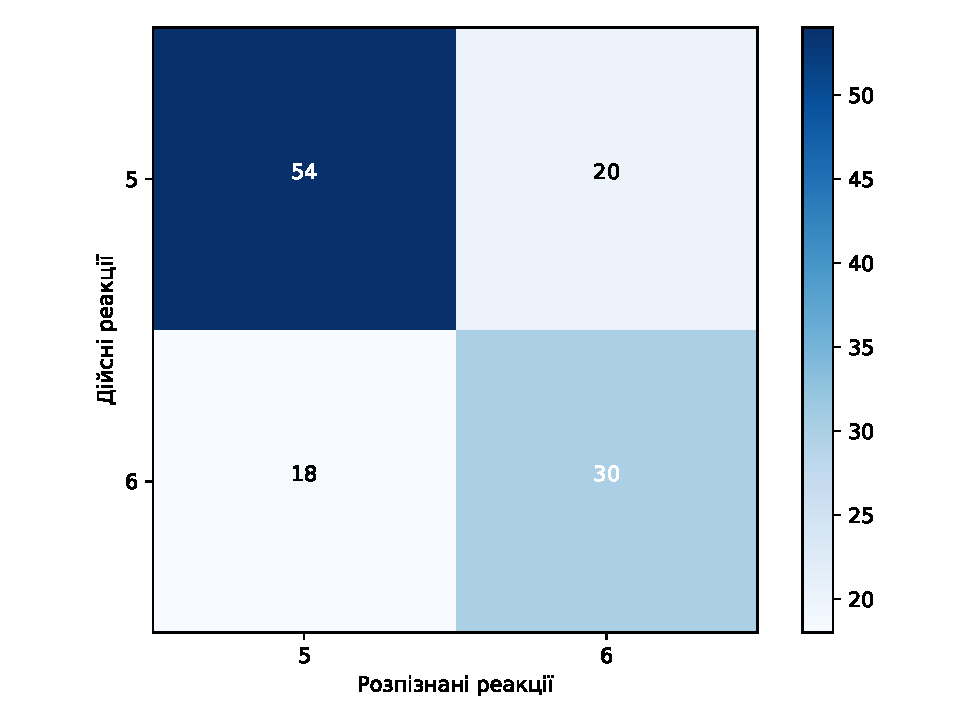
\includegraphics[width=0.3\linewidth]{confusion_matrix_data1_irs13_context_1}}
	\forloop{contextnumber}{3}{\value{contextnumber} < 14}{
		\subbottom[\arabic{contextnumber} \label{img:confusion_matrix_data1_irs13_context_\arabic{contextnumber}}]{%
			\includegraphics[width=0.3\linewidth]{confusion_matrix_data1_irs13_context_\arabic{contextnumber}}}
	}
	
	\caption{Матриці помилок розпізнавання по реакціях для різних контекстів першого набору даних методом ІРС розміром 1--3 (частина 1)}
	\label{img:confusion_matrix_data1_irs13_1}
\end{figure}
\begin{figure}
	\centering
	\forloop{contextnumber}{14}{\value{contextnumber} < 20}{
		\subbottom[\arabic{contextnumber} \label{img:confusion_matrix_data1_irs13_context_\arabic{contextnumber}}]{%
			\includegraphics[width=0.3\linewidth]{confusion_matrix_data1_irs13_context_\arabic{contextnumber}}}
	}
	
	\caption{Матриці помилок розпізнавання по реакціях для різних контекстів першого набору даних методом ІРС розміром 1--3 (частина 2)}
	\label{img:confusion_matrix_data1_irs13_2}
\end{figure}
\begin{figure}
	\centering
	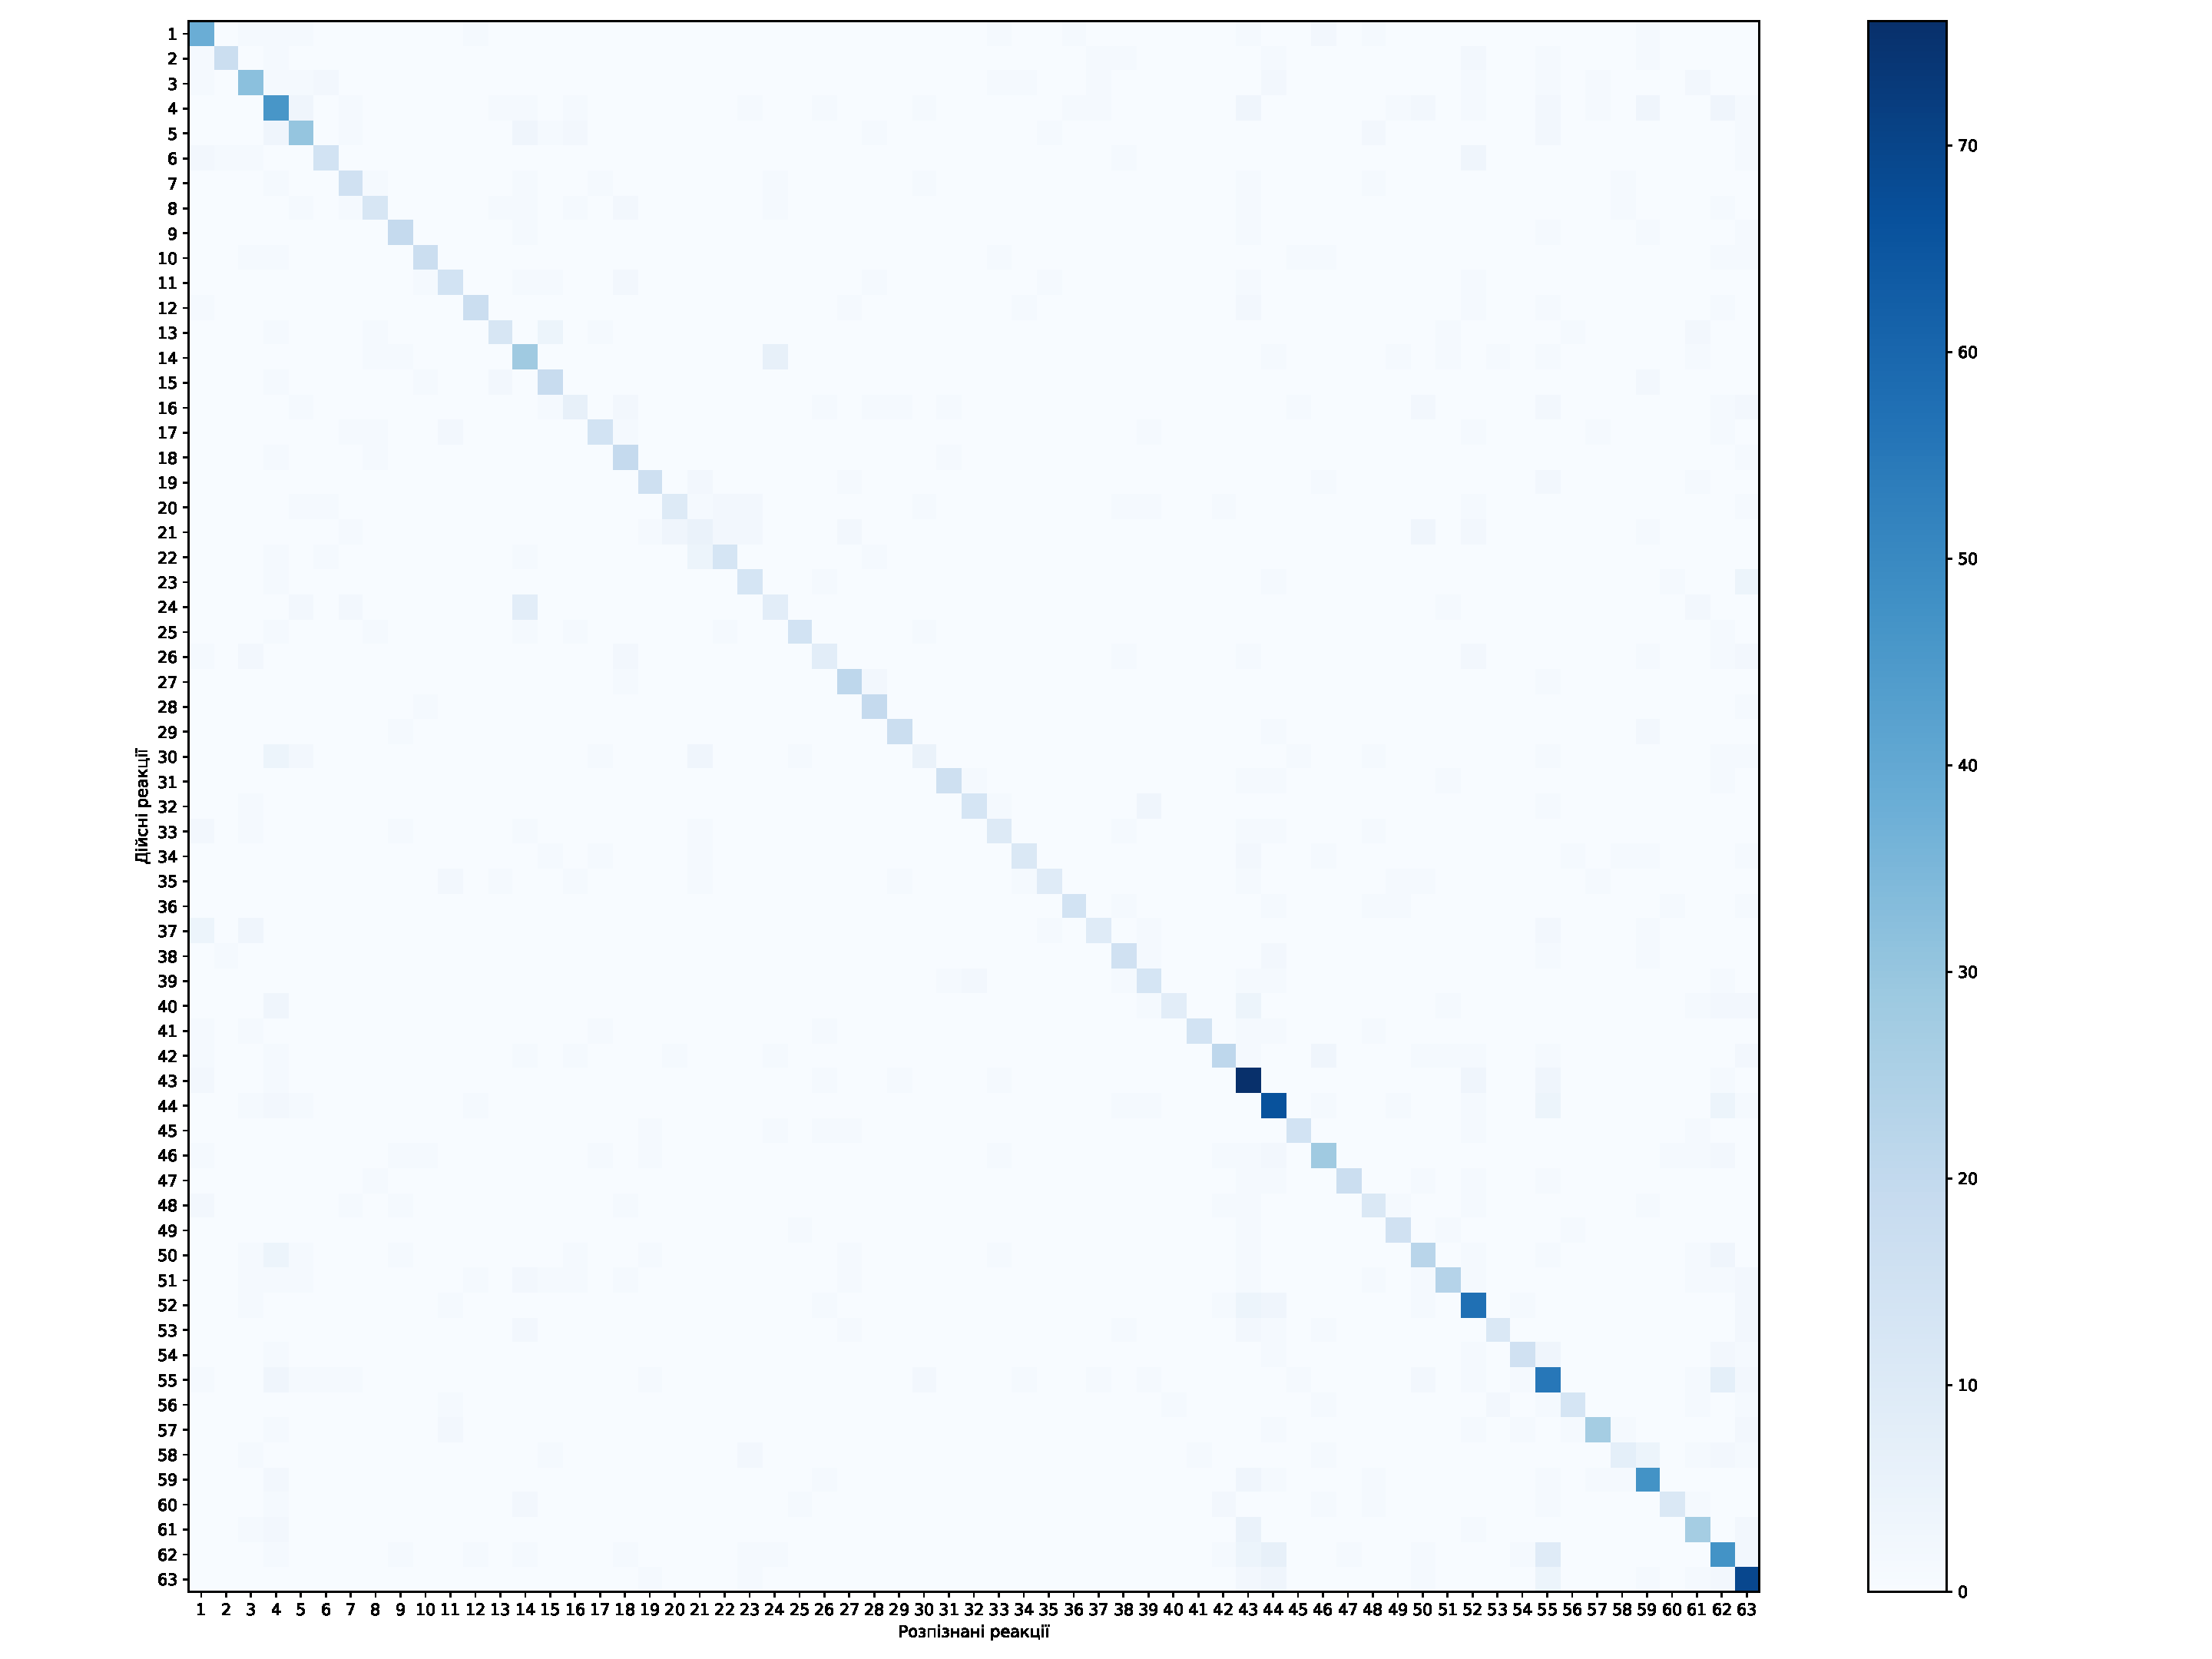
\includegraphics[width=\linewidth]{confusion_matrix_data1_cnn_context_20}
	\caption{Матриці помилок розпізнавання по реакціях по всій вибірці першого набору даних методом ІРС розміром 1--3}
	\label{img:confusion_matrix_data1_irs13_context_20}
\end{figure}

\begin{figure}
	\centering
	\subbottom[1 \label{img:confusion_matrix_data1_irs24_context_1}]{%
		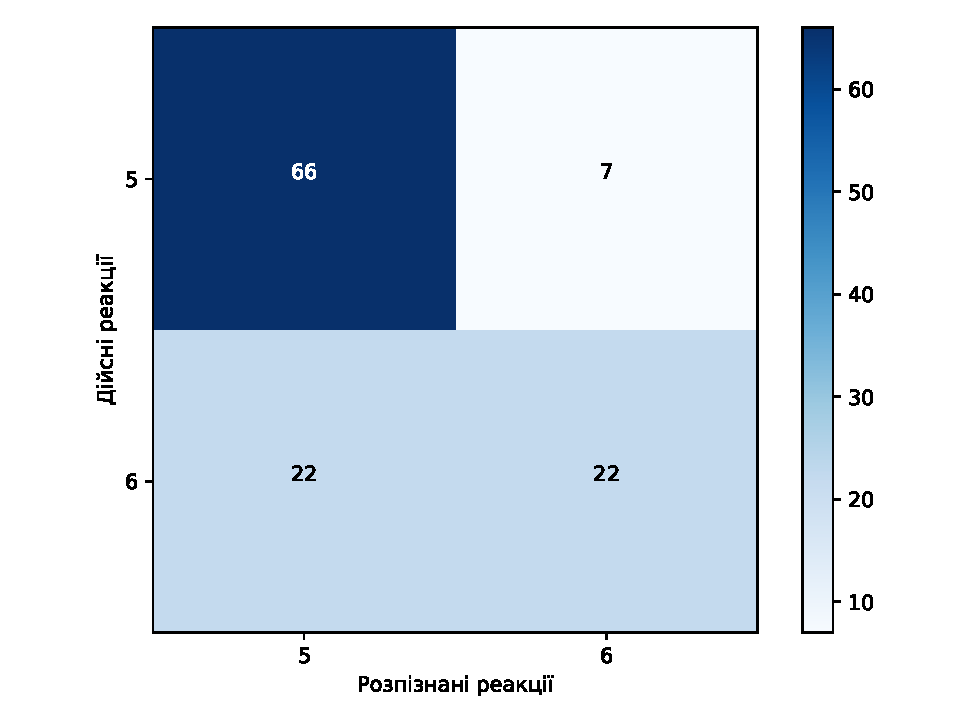
\includegraphics[width=0.3\linewidth]{confusion_matrix_data1_irs24_context_1}}
	\forloop{contextnumber}{3}{\value{contextnumber} < 14}{
		\subbottom[\arabic{contextnumber} \label{img:confusion_matrix_data1_irs24_context_\arabic{contextnumber}}]{%
			\includegraphics[width=0.3\linewidth]{confusion_matrix_data1_irs24_context_\arabic{contextnumber}}}
	}
	
	\caption{Матриці помилок розпізнавання по реакціях для різних контекстів першого набору даних методом ІРС розміром 2--4 (частина 1)}
	\label{img:confusion_matrix_data1_irs24_1}
\end{figure}
\begin{figure}
	\centering
	\forloop{contextnumber}{14}{\value{contextnumber} < 20}{
		\subbottom[\arabic{contextnumber} \label{img:confusion_matrix_data1_irs24_context_\arabic{contextnumber}}]{%
			\includegraphics[width=0.3\linewidth]{confusion_matrix_data1_irs24_context_\arabic{contextnumber}}}
	}
	
	\caption{Матриці помилок розпізнавання по реакціях для різних контекстів першого набору даних методом ІРС розміром 2--4 (частина 2)}
	\label{img:confusion_matrix_data1_irs24_2}
\end{figure}
\begin{figure}
	\centering
	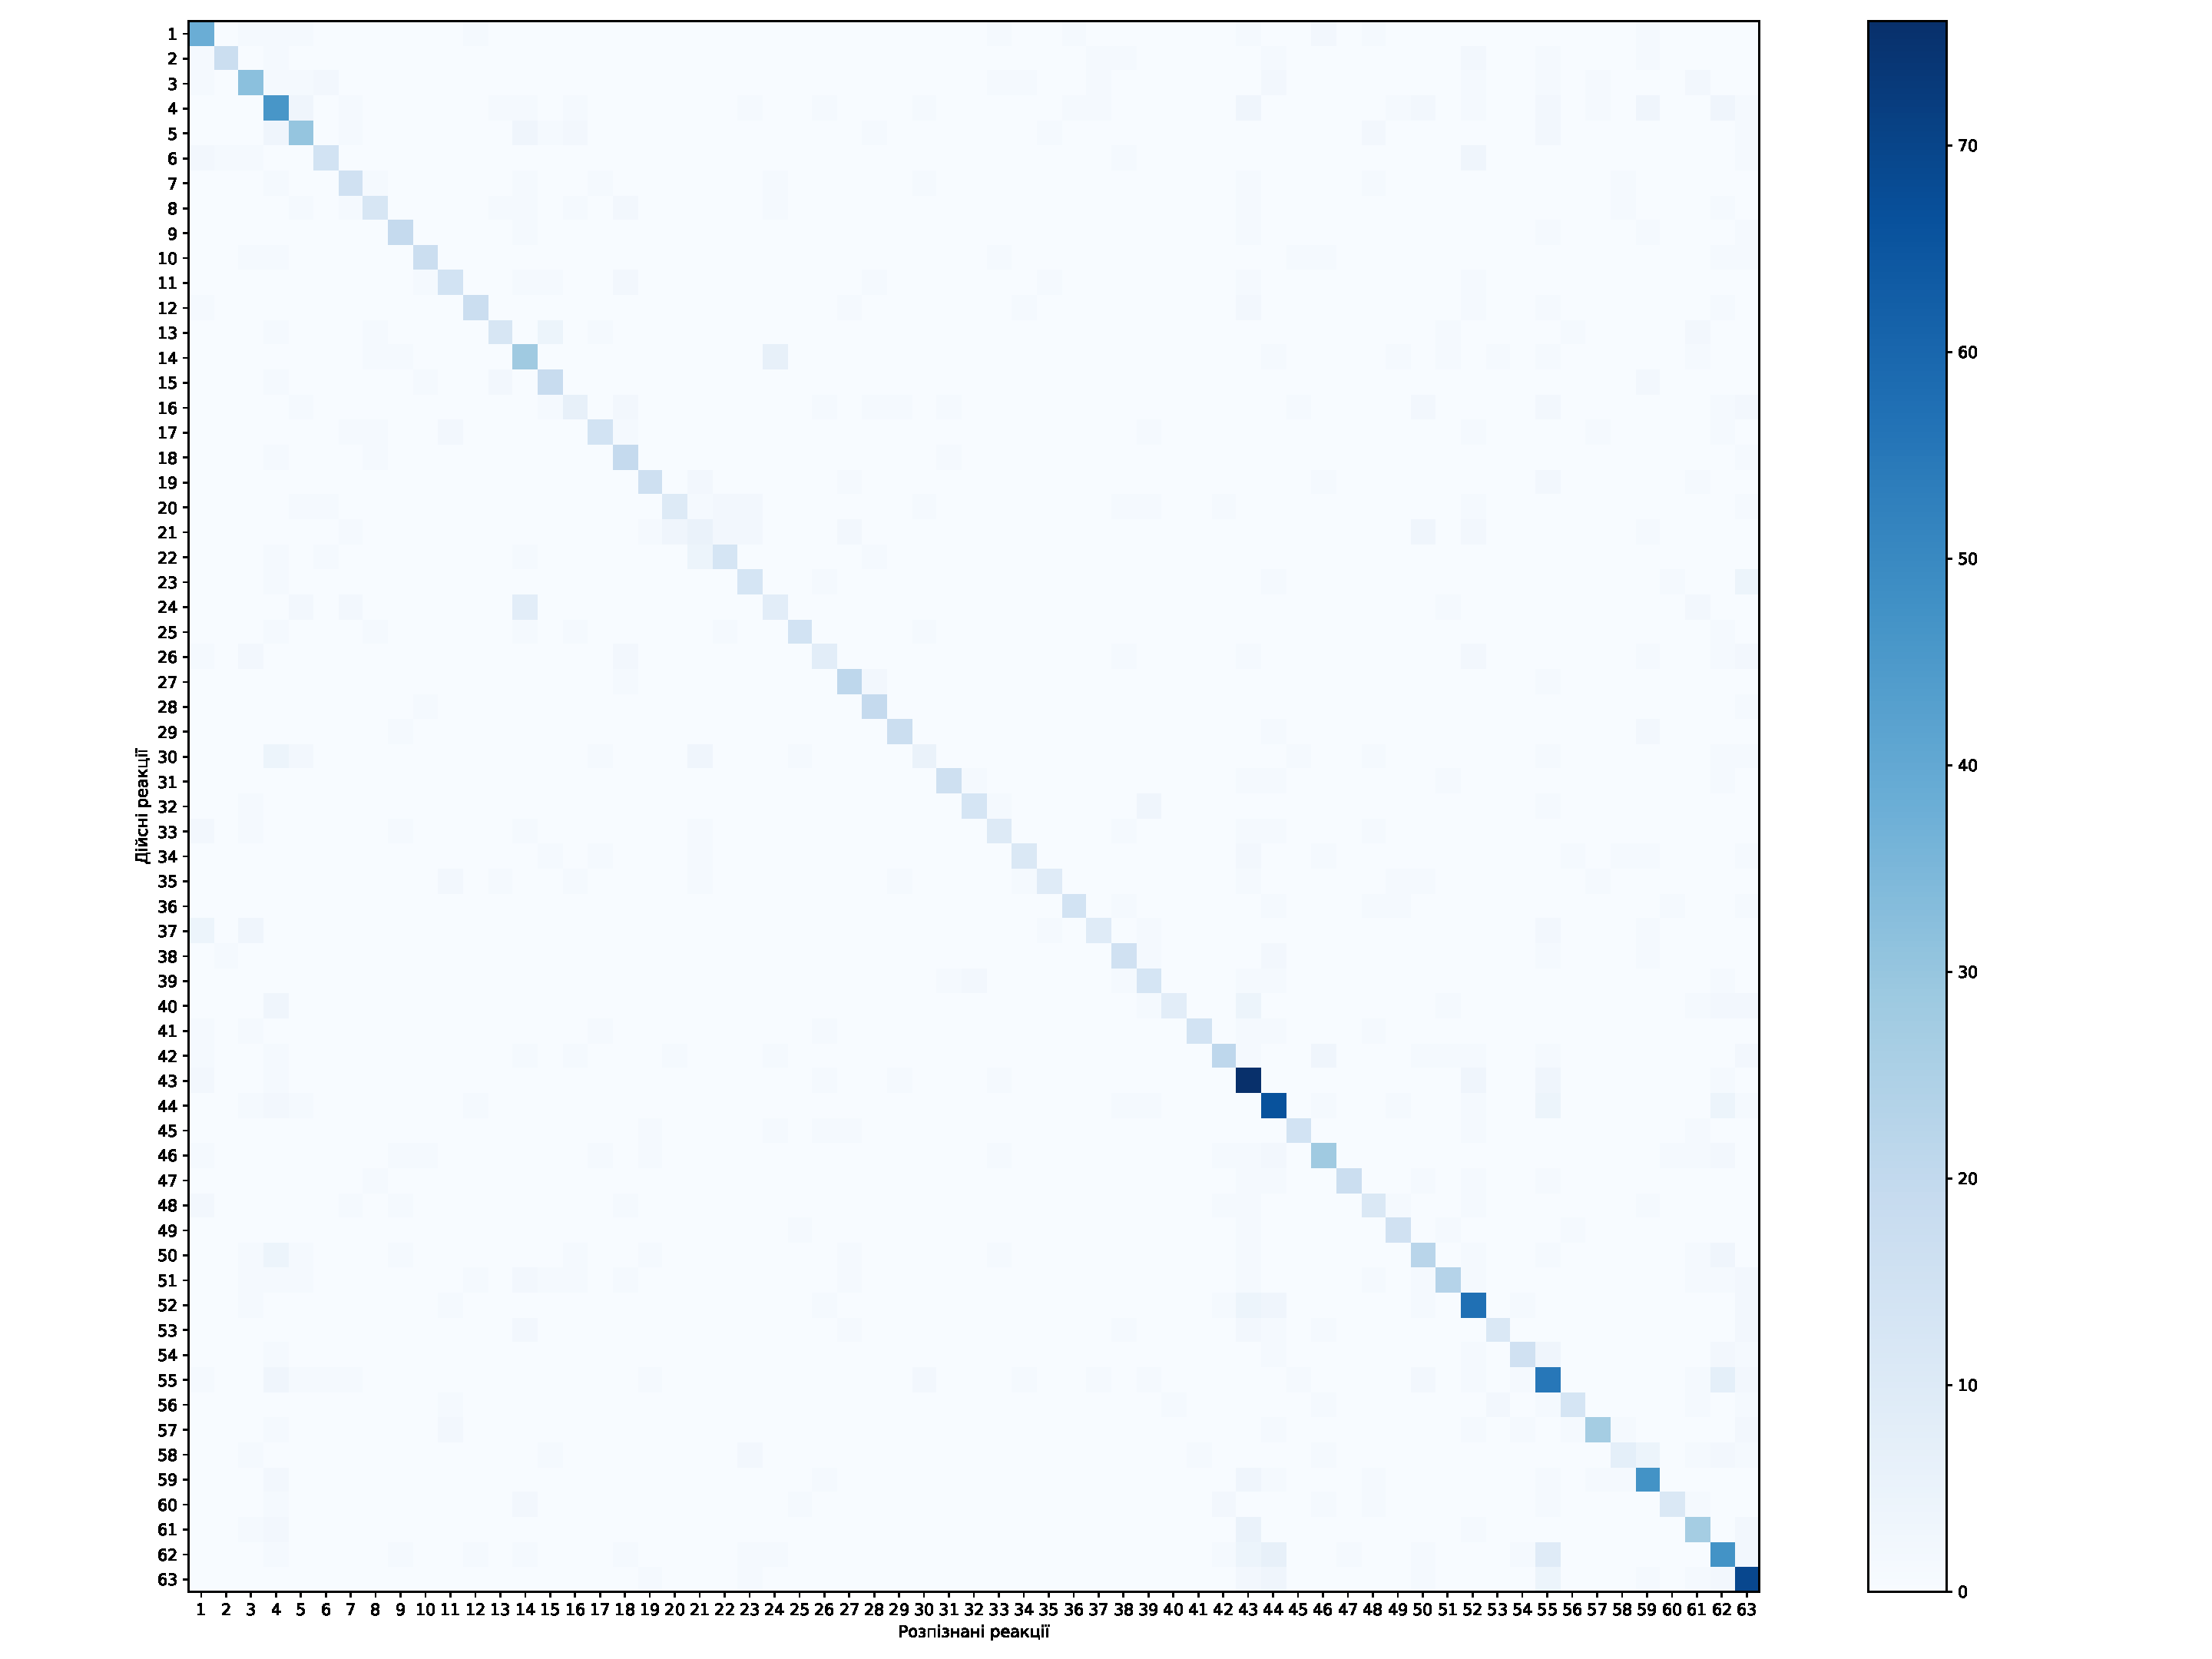
\includegraphics[width=\linewidth]{confusion_matrix_data1_cnn_context_20}
	\caption{Матриці помилок розпізнавання по реакціях по всій вибірці першого набору даних методом ІРС розміром 2--4}
	\label{img:confusion_matrix_data1_irs24_context_20}
\end{figure}

\begin{figure}
	\centering
	\subbottom[1 \label{img:confusion_matrix_data1_cnn_context_1}]{%
		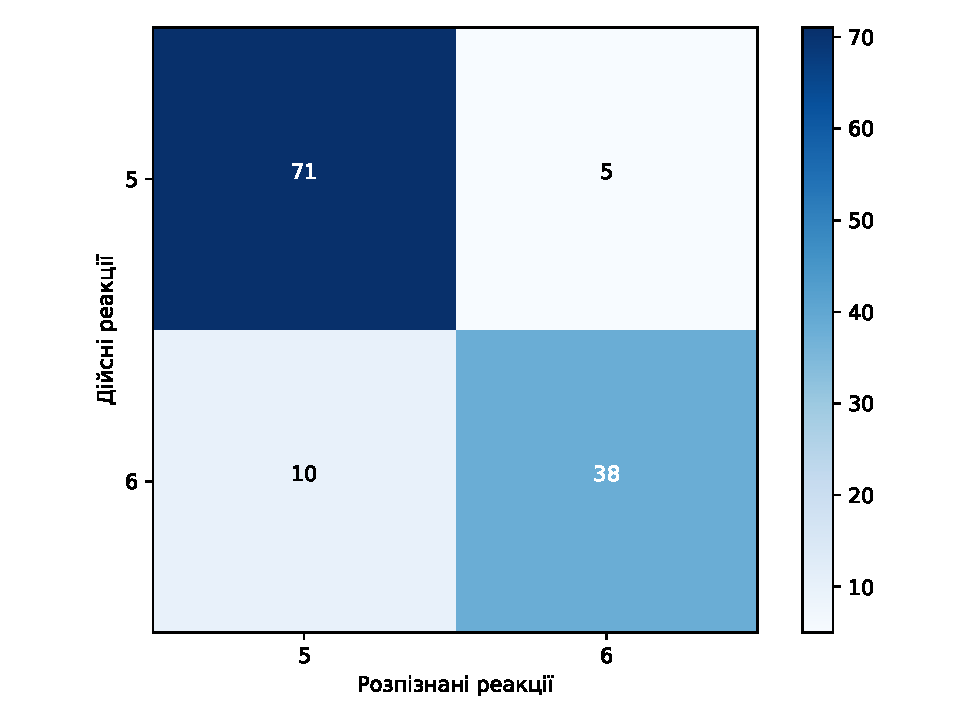
\includegraphics[width=0.3\linewidth]{confusion_matrix_data1_cnn_context_1}}
	\forloop{contextnumber}{3}{\value{contextnumber} < 14}{
		\subbottom[\arabic{contextnumber} \label{img:confusion_matrix_data1_cnn_context_\arabic{contextnumber}}]{%
			\includegraphics[width=0.3\linewidth]{confusion_matrix_data1_cnn_context_\arabic{contextnumber}}}
	}
	
	\caption{Матриці помилок розпізнавання по реакціях для різних контекстів першого набору даних методом ЗНМ (частина 1)}
	\label{img:confusion_matrix_data1_cnn_1}
\end{figure}
\begin{figure}
	\centering
	\forloop{contextnumber}{14}{\value{contextnumber} < 20}{
		\subbottom[\arabic{contextnumber} \label{img:confusion_matrix_data1_cnn_context_\arabic{contextnumber}}]{%
			\includegraphics[width=0.3\linewidth]{confusion_matrix_data1_cnn_context_\arabic{contextnumber}}}
	}
	
	\caption{Матриці помилок розпізнавання по реакціях для різних контекстів першого набору даних методом ЗНМ (частина 2)}
	\label{img:confusion_matrix_data1_cnn_2}
\end{figure}
\begin{figure}
	\centering
	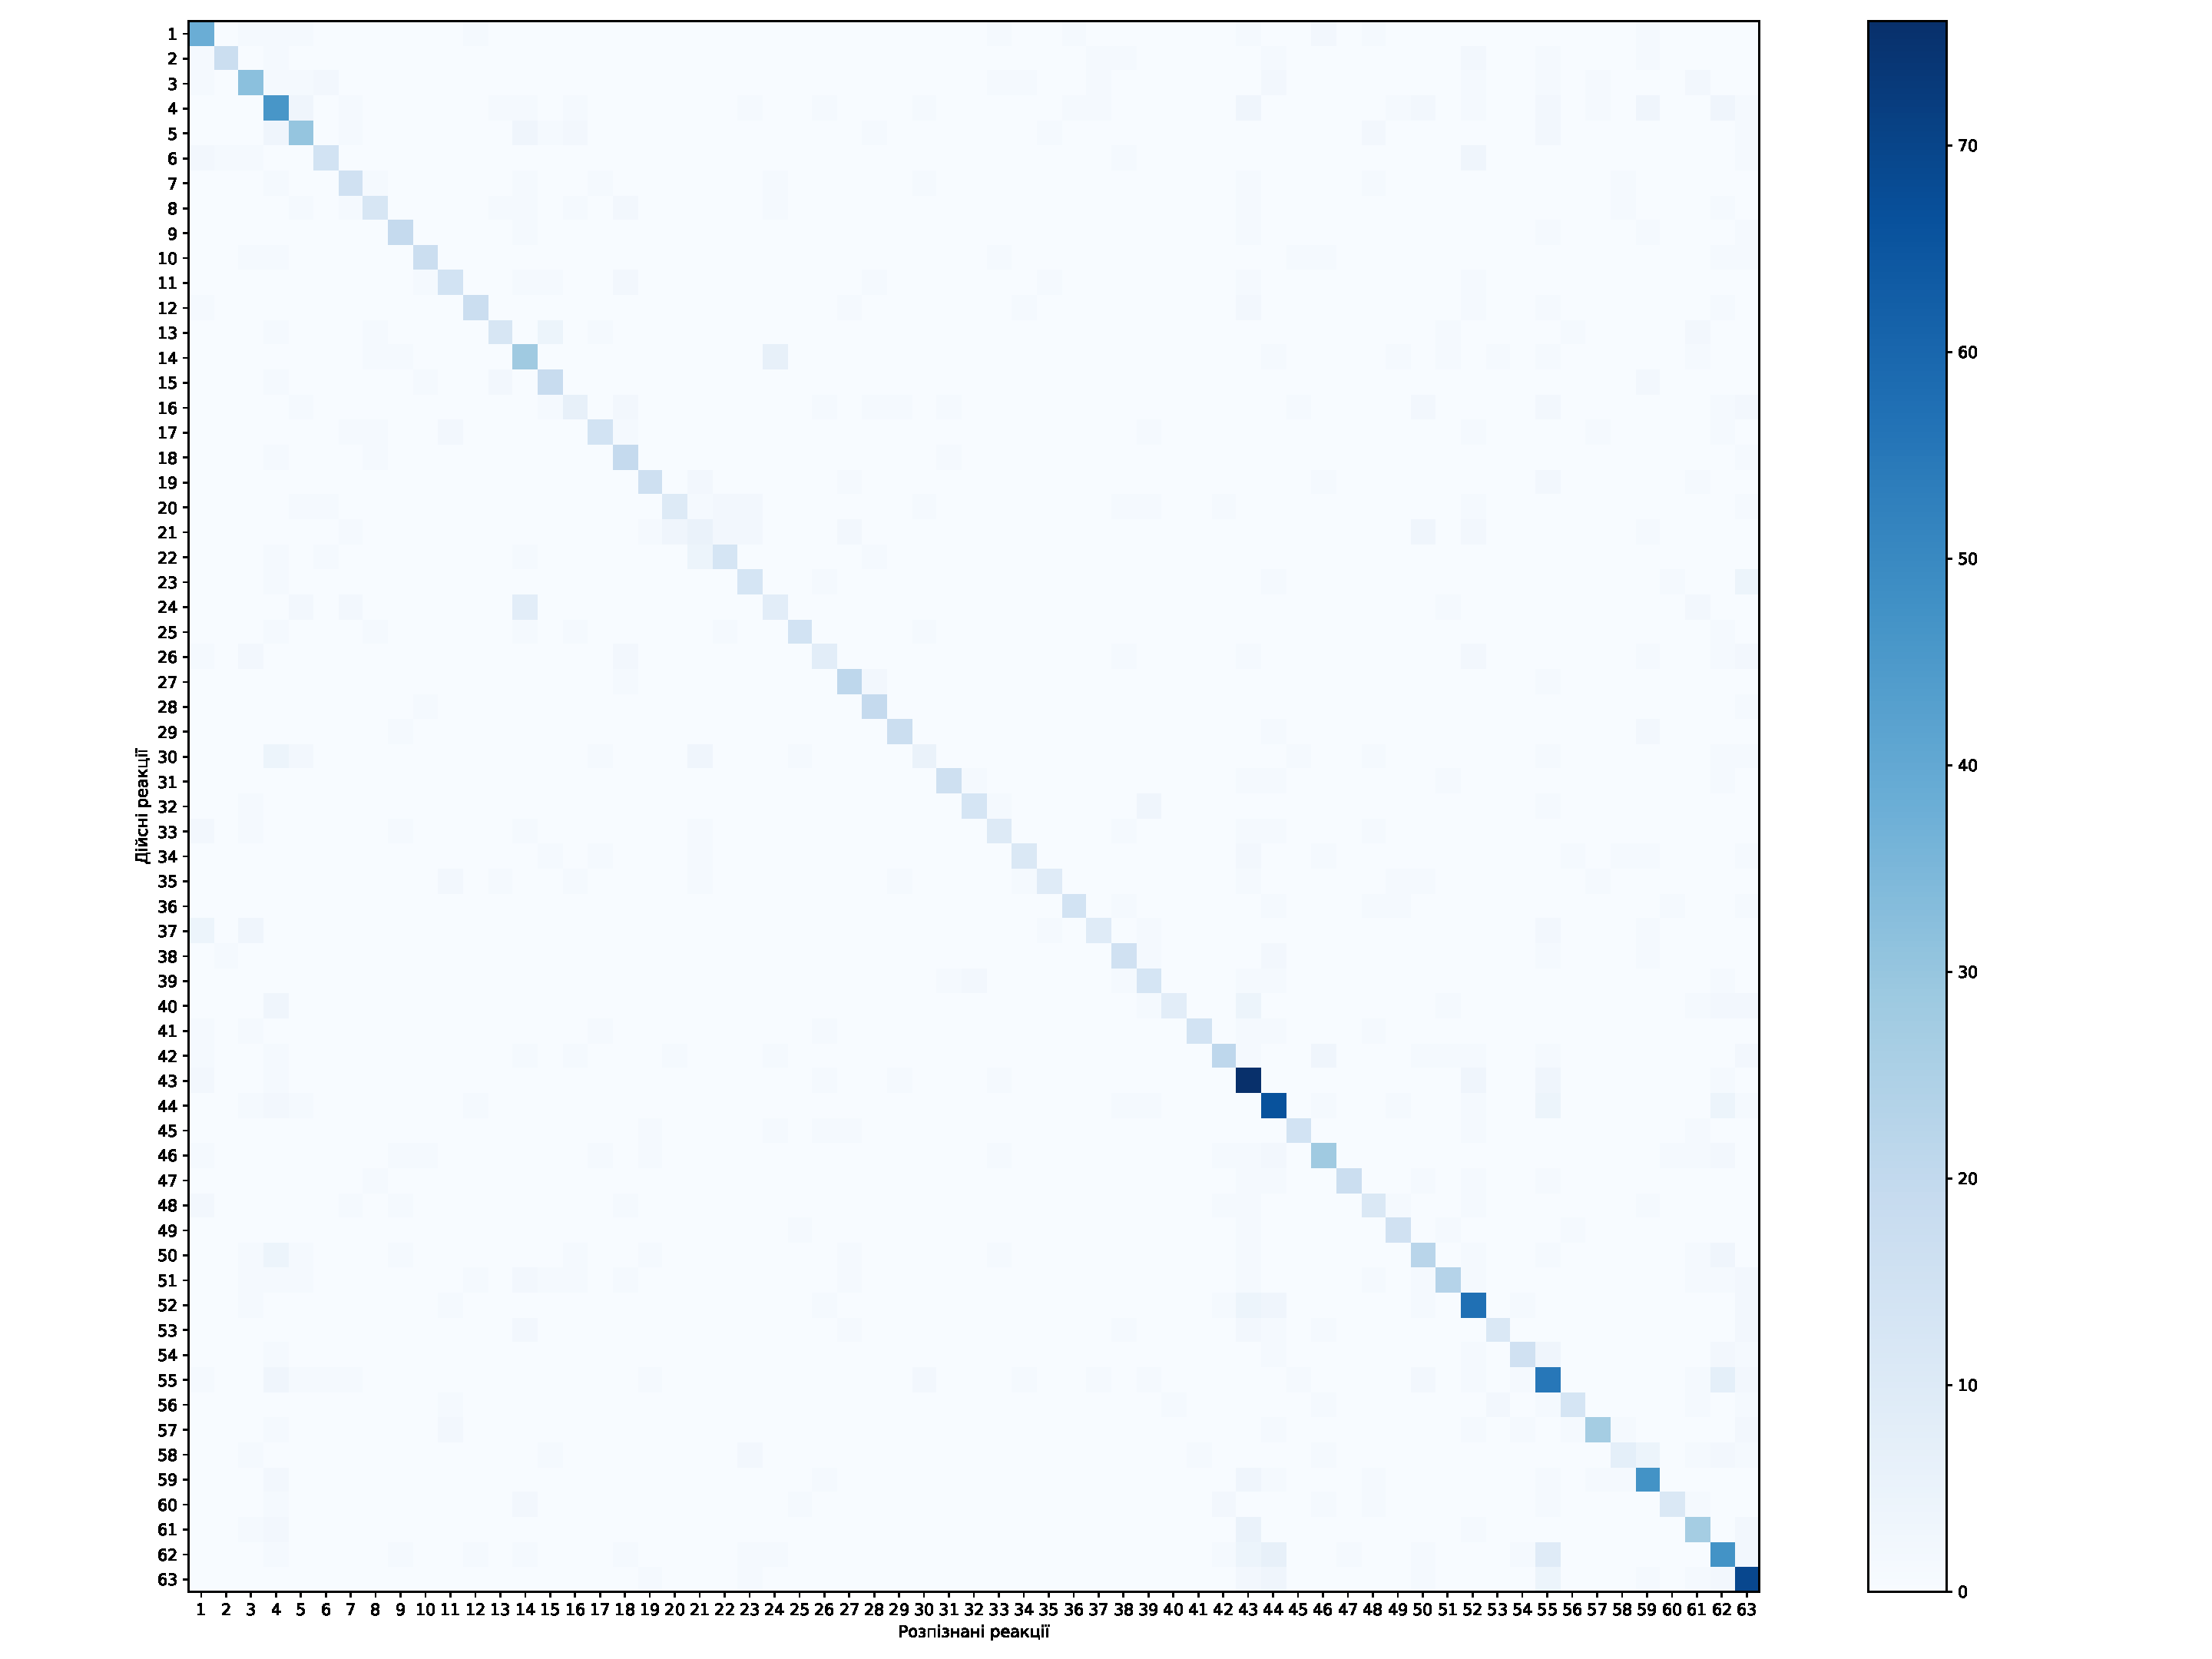
\includegraphics[width=\linewidth]{confusion_matrix_data1_cnn_context_20}
	\caption{Матриці помилок розпізнавання по реакціях по всій вибірці першого набору даних методом ЗНМ}
	\label{img:confusion_matrix_data1_cnn_context_20}
\end{figure}

\begin{figure}
	\centering
	\subbottom[1 \label{img:confusion_matrix_data3_irs13_context_1}]{%
		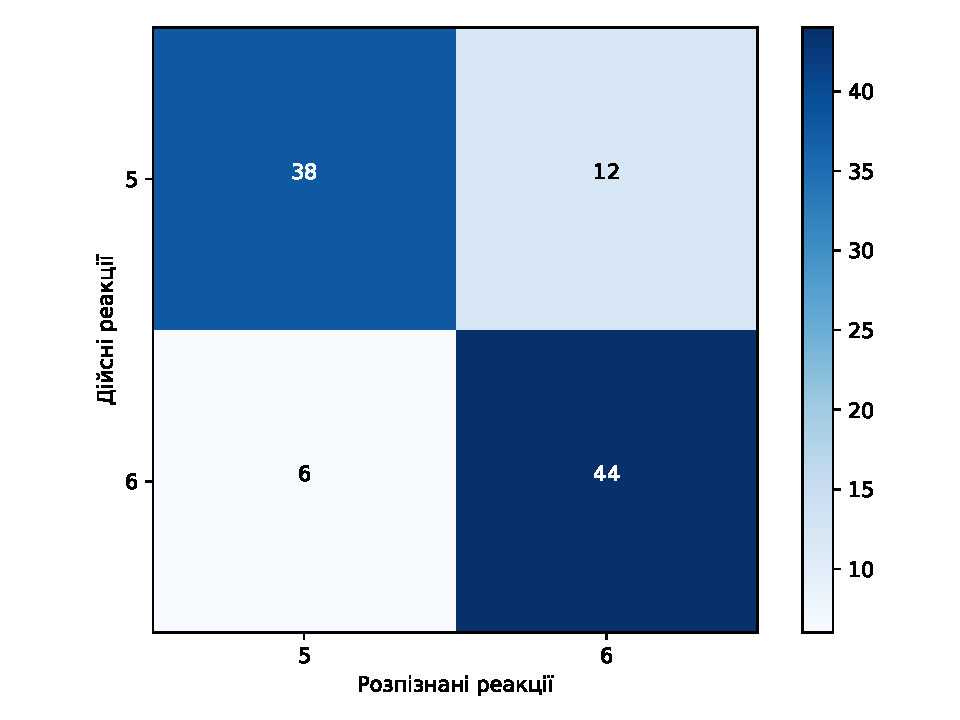
\includegraphics[width=0.3\linewidth]{confusion_matrix_data3_irs13_context_1}}
	\forloop{contextnumber}{3}{\value{contextnumber} < 14}{
		\subbottom[\arabic{contextnumber} \label{img:confusion_matrix_data3_irs13_context_\arabic{contextnumber}}]{%
			\includegraphics[width=0.3\linewidth]{confusion_matrix_data3_irs13_context_\arabic{contextnumber}}}
	}
	
	\caption{Матриці помилок розпізнавання по реакціях для різних контекстів третього набору даних методом ІРС розміром 1--3 (частина 1)}
	\label{img:confusion_matrix_data3_irs13_1}
\end{figure}
\begin{figure}
	\centering
	\forloop{contextnumber}{14}{\value{contextnumber} < 20}{
		\subbottom[\arabic{contextnumber} \label{img:confusion_matrix_data3_irs13_context_\arabic{contextnumber}}]{%
			\includegraphics[width=0.3\linewidth]{confusion_matrix_data3_irs13_context_\arabic{contextnumber}}}
	}
	
	\caption{Матриці помилок розпізнавання по реакціях для різних контекстів третього набору даних методом ІРС розміром 1--3 (частина 2)}
	\label{img:confusion_matrix_data3_irs13_2}
\end{figure}
\begin{figure}
	\centering
	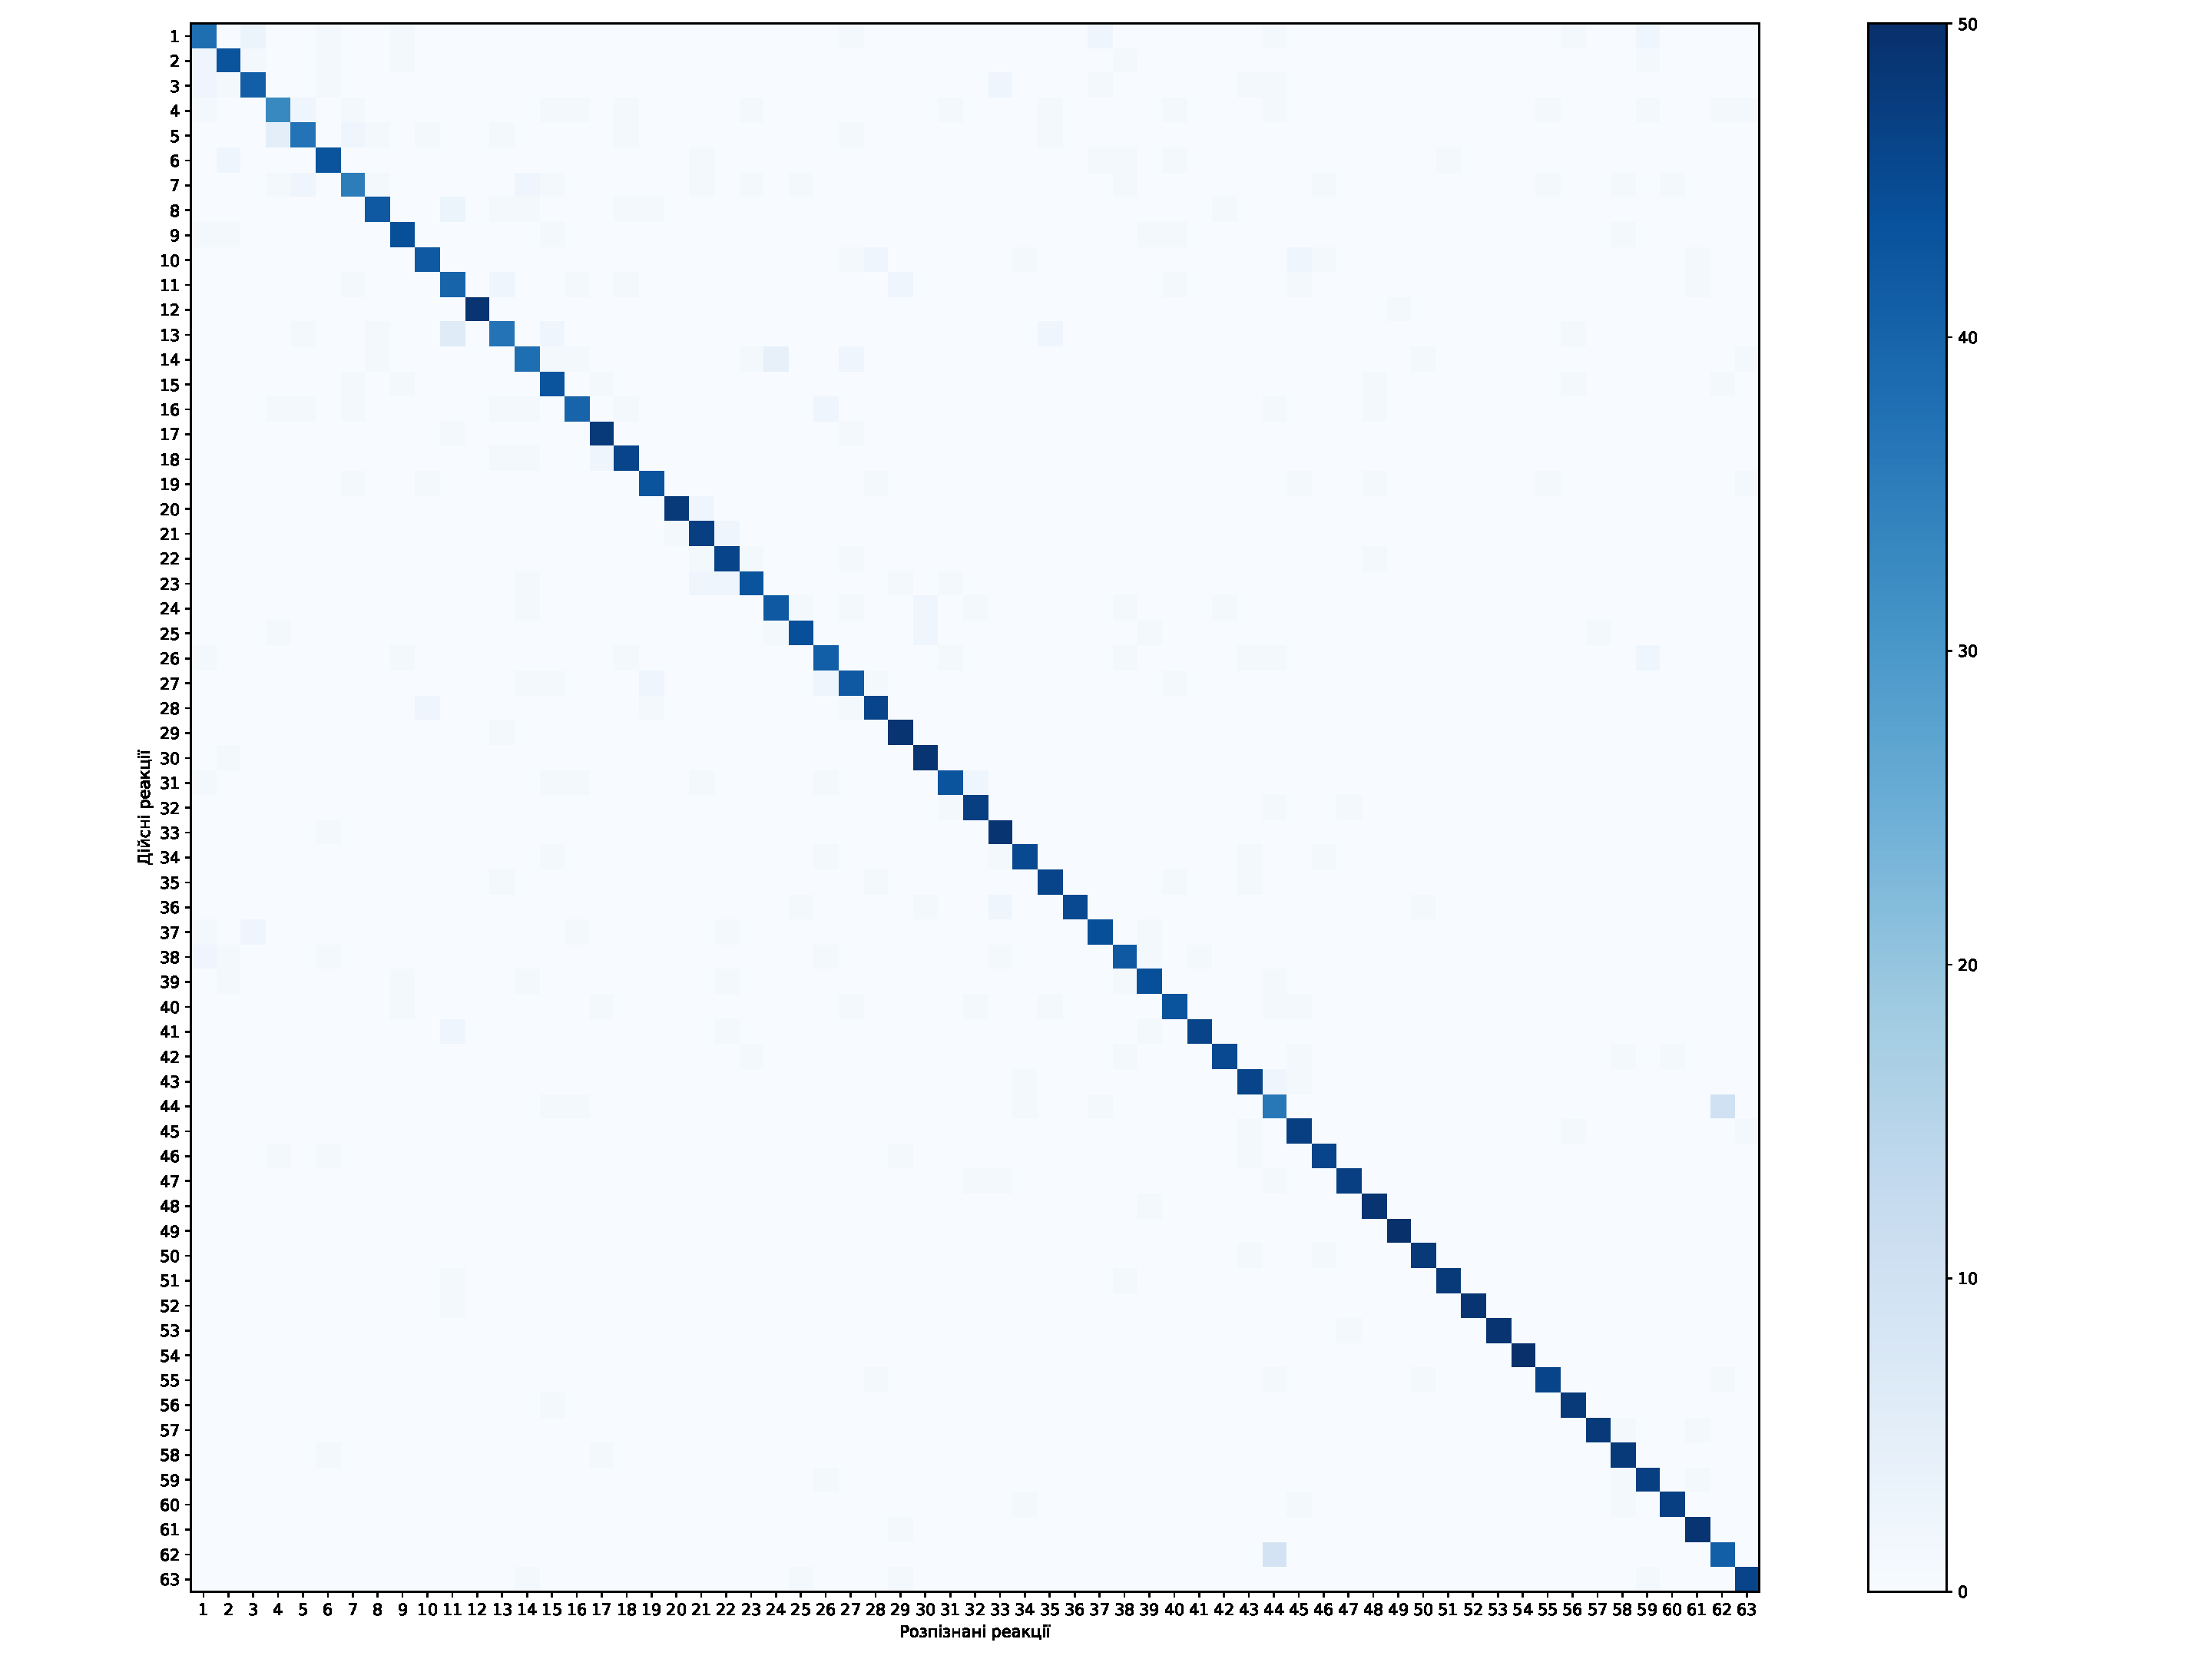
\includegraphics[width=\linewidth]{confusion_matrix_data3_cnn_context_20}
	\caption{Матриці помилок розпізнавання по реакціях по всій вибірці третього набору даних методом ІРС розміром 1--3}
	\label{img:confusion_matrix_data3_irs13_context_20}
\end{figure}

\begin{figure}
	\centering
	\subbottom[1 \label{img:confusion_matrix_data3_irs24_context_1}]{%
		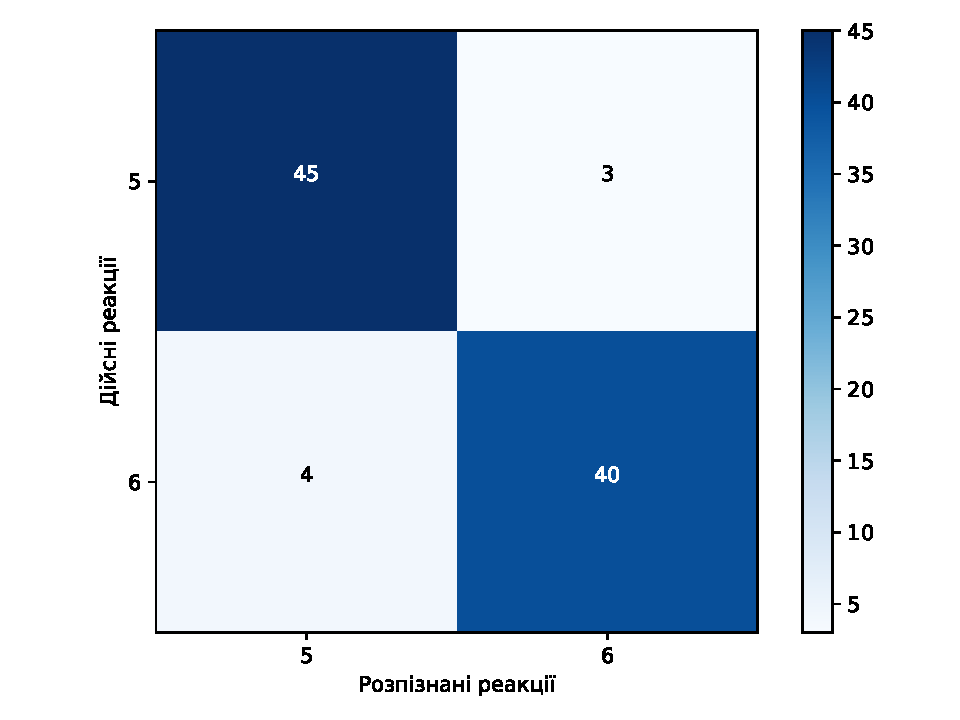
\includegraphics[width=0.3\linewidth]{confusion_matrix_data3_irs24_context_1}}
	\forloop{contextnumber}{3}{\value{contextnumber} < 14}{
		\subbottom[\arabic{contextnumber} \label{img:confusion_matrix_data3_irs24_context_\arabic{contextnumber}}]{%
			\includegraphics[width=0.3\linewidth]{confusion_matrix_data3_irs24_context_\arabic{contextnumber}}}
	}
	
	\caption{Матриці помилок розпізнавання по реакціях для різних контекстів третього набору даних методом ІРС розміром 2--4 (частина 1)}
	\label{img:confusion_matrix_data3_irs24_1}
\end{figure}
\begin{figure}
	\centering
	\forloop{contextnumber}{14}{\value{contextnumber} < 20}{
		\subbottom[\arabic{contextnumber} \label{img:confusion_matrix_data3_irs24_context_\arabic{contextnumber}}]{%
			\includegraphics[width=0.3\linewidth]{confusion_matrix_data3_irs24_context_\arabic{contextnumber}}}
	}
	
	\caption{Матриці помилок розпізнавання по реакціях для різних контекстів третього набору даних методом ІРС розміром 2--4 (частина 2)}
	\label{img:confusion_matrix_data3_irs24_2}
\end{figure}
\begin{figure}
	\centering
	\includegraphics[width=\linewidth]{confusion_matrix_data3_cnn_context_20}
	\caption{Матриці помилок розпізнавання по реакціях по всій вибірці третього набору даних методом ІРС розміром 2--4}
	\label{img:confusion_matrix_data3_irs24_context_20}
\end{figure}

\begin{figure}
	\centering
	\subbottom[1 \label{img:confusion_matrix_data3_cnn_context_1}]{%
		\includegraphics[width=0.3\linewidth]{confusion_matrix_data3_cnn_context_1}}
	\forloop{contextnumber}{3}{\value{contextnumber} < 14}{
		\subbottom[\arabic{contextnumber} \label{img:confusion_matrix_data3_cnn_context_\arabic{contextnumber}}]{%
			\includegraphics[width=0.3\linewidth]{confusion_matrix_data3_cnn_context_\arabic{contextnumber}}}
	}
	
	\caption{Матриці помилок розпізнавання по реакціях для різних контекстів третього набору даних методом ЗНМ (частина 1)}
	\label{img:confusion_matrix_data3_cnn_1}
\end{figure}
\begin{figure}
	\centering
	\forloop{contextnumber}{14}{\value{contextnumber} < 20}{
		\subbottom[\arabic{contextnumber} \label{img:confusion_matrix_data3_cnn_context_\arabic{contextnumber}}]{%
			\includegraphics[width=0.3\linewidth]{confusion_matrix_data3_cnn_context_\arabic{contextnumber}}}
	}
	
	\caption{Матриці помилок розпізнавання по реакціях для різних контекстів третього набору даних методом ЗНМ (частина 2)}
	\label{img:confusion_matrix_data3_cnn_2}
\end{figure}
\begin{figure}
	\centering
	\includegraphics[width=\linewidth]{confusion_matrix_data3_cnn_context_20}
	\caption{Матриці помилок розпізнавання по реакціях по всій вибірці третього набору даних методом ЗНМ}
	\label{img:confusion_matrix_data3_cnn_context_20}
\end{figure}

\chapter{Довідка про впровадження} \label{AppendixС}

\begin{center}
	\includegraphics[width=\linewidth]{190104170842}
\end{center}

\chapter{Список публікацій здобувача за темою дисертації та відомості про апробацію результатів дисертації}

\printbibliography[heading=pubsubgroup, keyword=biblioauthorvak, section=1,title={Список публікацій здобувача в яких опубліковані основні наукові результати
	дисертації:}]%
\printbibliography[heading=pubsubgroup, keyword=biblioauthorconf, section=1,title={Список публікацій здобувача, які засвідчують апробацію матеріалів
	дисертації:}]%
\printbibliography[heading=pubsubgroup, keyword=biblioauthornotvak, section=1,title={Список публікацій здобувача, які додатково відображають наукові
	результати дисертації:}]%

\begin{center}
	\textit{Основні положення дисертаційної роботи були апробовані у наступних міжнародних науково-технічних конференціях}
\end{center}

\begin{itemize}
	\item XVII Міжнародна науково-технічна конференція «Системний аналіз та інформаційні технології» (м. Київ, 22--25 червня 2015 р.)
	\item XII Міжнародна конференція «Управління проектами у розвитку суспільства», тема: «Комплексне управління проектами розвитку в умовах нестабільного оточення» (м. Київ, 21-23 травня 2015 р.)
	\item ІІІ Міжнародна науково-практична конференція «Інформаційні технології та взаємодії» (м. Київ, 8--10 листопада 2016 р.)
	\item 16th EAGE International Conference on Geoinformatics - Theoretical and Applied Aspects (м. Київ, 15--17 травня 2017 р.)
	\item ІV Міжнародна науково-практична конференція «Інформаційні технології та взаємодії» (м. Київ, 8--10 листопада 2017 р.)
\end{itemize}        % Приложения

%\begin{figure}
	\centering
	\includegraphics [width=.5\linewidth] {hmm}
	\caption{Топологія прихованих Марковських моделей з трьома станами}
	\label{img:hmm}
\end{figure}
\begin{figure}
	\centering
	\includegraphics [width=\linewidth] {voice_interaction_schema}
	\caption{Схема голосової взаємодії субʼєктів дистрибуції}
	\label{img:voice_interaction_schema}
\end{figure}
\begin{figure}
	\centering
	\includegraphics [width=.5\linewidth] {rgsu_concept}
	\caption{Схема узагальненої структури рефлекторних систем голосового управління}
	\label{img:rgsu_concept}
\end{figure}
\begin{figure}
	\centering
	\includegraphics [width=1\linewidth] {01_simplest_positive_scenario}
	\caption{Найпростіше дерево сценаріїв}
	\label{img:01_simplest_positive_scenario}
\end{figure}
\begin{figure}
	\centering
	\includegraphics [width=1\linewidth] {02_simplest_positive_scenario_vertical}
	\caption{Вертикальний розподіл найпростішого дерева сценаріїв}
	\label{img:02_simplest_positive_scenario_vertical}
\end{figure}
\begin{figure}
	\centering
	\includegraphics [width=1\linewidth] {03_positive_scenario_with_conformation}
	\caption{Позитивне дерево сценаріїв з підтвердженням}
	\label{img:03_positive_scenario_with_conformation}
\end{figure}
\begin{figure}
	\centering
	\includegraphics [width=1\linewidth] {04_first_negative_scenario_with_conformation}
	\caption{Перший варіант дерева сценаріїв з негативними інцидентами}
	\label{img:04_first_negative_scenario_with_conformation}
\end{figure}
\begin{figure}
	\centering
	\includegraphics [width=1\linewidth] {05_simple_negative_scenario_with_conformation}
	\caption{Спрощений варіант дерева сценаріїв з негативними інцидентами}
	\label{img:05_simple_negative_scenario_with_conformation}
\end{figure}
\begin{figure}
	\centering
	\includegraphics [width=1\linewidth] {06_simple_negative_scenario_with_rollback}
	\caption{Варіант дерева сценаріїв з негативними інцидентами та відбоєм}
	\label{img:06_simple_negative_scenario_with_rollback}
\end{figure}
\begin{figure}
	\centering
	\includegraphics [width=1\linewidth] {07_simple_point_scenario}
	\caption{Частина дерева сценаріїв етапу <<точка доставки>>}
	\label{img:07_simple_point_scenario}
\end{figure}
\begin{figure}
	\centering
	\includegraphics [width=1\linewidth] {07_simple_point_scenario_horizontal}
	\caption{Частина дерева сценаріїв етапу <<точка доставки>> в горизонтальному розподілі}
	\label{img:07_simple_point_scenario_horizontal}
\end{figure}
\begin{figure}
	\centering
	\includegraphics [width=1\linewidth] {08_complete_point_scenario}
	\caption{Частина дерева сценаріїв етапу <<точка доставки>> з усіма негативними інцидентами}
	\label{img:08_complete_point_scenario}
\end{figure}
\begin{figure}
	\centering
	\includegraphics [width=1\linewidth] {08_complete_point_scenario_with_other}
	\caption{Частина дерева сценаріїв етапу <<точка доставки>> з усіма негативними інцидентами та урахуванням інших непередбачених подій}
	\label{img:08_complete_point_scenario_with_other}
\end{figure}
\begin{figure} 
	\centering
	\includegraphics [width=1\linewidth] {09_complete_point_scenario_with_rollback}
	\caption{Частина дерева сценаріїв етапу "точка доставки" з усіма негативними інцидентами та відбоєм із діалогового режиму}
	\label{img:09_complete_point_scenario_with_rollback}
\end{figure}
\begin{figure}
	\centering
	\includegraphics [width=1\linewidth] {10_point_scenario_with_enchantment}
	\caption{Частина дерева сценаріїв етапу <<точка доставки>> з додатковими функціями}
	\label{img:10_point_scenario_with_enchantment}
\end{figure}
\begin{figure}
	\centering
	\includegraphics [width=.8\linewidth] {11_complete_road_scenario}
	\caption{Частина дерева сценаріїв етапу <<дорога>>}
	\label{img:11_complete_road_scenario}
\end{figure}
\begin{figure}
	\centering
	\includegraphics [width=.8\linewidth] {12_complete_depot_scenario}
	\caption{Частина дерева сценаріїв етапу <<склад>>}
	\label{img:12_complete_depot_scenario}
\end{figure}
\begin{figure}
	\centering
	\includegraphics [width=1\linewidth] {13_complete_scenario_graph}
	\caption{Повне дерево сценаріїв всіх етапів}
	\label{img:13_complete_scenario_graph}
\end{figure}
\begin{mytable*}{ | c | l | }%
	{Різні варіанти стимулів з дерева сценаріїв}%
	{\label{tbl:scenario_commands}}%
	{№ & Варіанти стимулу}
	
	1 & Виїхав зі складу \\
	\hline
	2 & Прибув у точку, починаю виконання \\
	\hline
	3 & Точка виконана успішно \\
	\hline
	4 & Переходжу до наступної точки \\
	\hline
	5 & Так \\
	\hline
	6 & Ні \\
	\hline
	7 & Точка не виконана \\
	\hline
	8 & Відбій, я ще не на місці \\
	\hline
	9 & Клієнт відсутній на місці \\
	\hline
	10 & Немає можливості виконати доставку  \\
	\hline
	11 & Помилка в замовленні \\
	\hline
	12 & Відмова клієнта прийняти товар \\
	\hline
	13 & Клієнт забув про доставку \\
	\hline
	14 & Клієнт не зміг бути вчасно \\
	\hline
	15 & Немає на місці, немає звʼязку \\
	\hline
	16 & Невчасний приїзд на точку доставку \\
	\hline
	17 & Не працює ліфт \\
	\hline
	18 & Закрито доступ до приміщення клієнта \\
	\hline
	19 & У клиента відсутні необхідні документи \\
	\hline
	20 & Не замовляли взагалі \\
	\hline
	21 & Замовляли на інший день \\
	\hline
	22 & Замовляли на іншу адресу \\
	\hline
	23 & Замовляли на інший час \\
	\hline
	24 & Замовляли інший товар \\
	\hline
	25 & Відмова на місці \\
	\hline
	26 & Немає грошей \\
	\hline
	27 & Пошкоджений або відсутній товар \\
	\hline
	28 & Часткове виконання замовлення \\
	\hline
	29 & Задвоєне замовлення, половина повертається \\
	\hline
	30 & У документах зазначено товар, який клієнт не замовляв \\
	\hline
	31 & Інше \\
	\hline
	32 & Показати маршрутний лист \\
	\hline
	33 & Показати мапу маршруту \\
	\hline
	34 & Показати інформацію про точку \\
	\hline
	35 & Набрати диспетчера \\
	\hline
	36 & Набрати клієнта \\
	\hline
	37 & Затримки у русі \\
	\hline
	38 & Проблемна точка \\
	\hline
	39 & Неможливо досягти точку \\
	\hline
	40 & Неможливо продовжувати маршрут \\
	\hline
	41 & \# хвилин \\
	\hline
	42 & Транспортний затор \\
	\hline
	43 & Тимчасово перекриті дороги \\
	\hline
	44 & Помилка мапи, дорога не існує \\
	\hline
	45 & Транспортний засіб попав у ДТП \\
	\hline
	46 & Поломка ТЗ на маршруті \\
	\hline
	47 & Складні погодні умови \\
	\hline
	48 & Помилка геокодування \\
	\hline
	49 & Похибка при складанні маршруту \\
	\hline
	50 & Підʼїзд до будинку з іншої вулиці \\
	\hline
	51 & Немає підʼїзду до будинку \\
	\hline
	52 & Неправильна адреса, або недостатньо інформації \\
	\hline
	53 & Не було місця для парковки \\
	\hline
	54 & Авто не пройшло по габаритам \\
	\hline
	55 & Затримка на складі \\
	\hline
	56 & Проблеми з вантажем \\
	\hline
	57 & Проблеми з ТЗ \\
	\hline
	58 & Запізнення прибуття на склад \\
	\hline
	59 & Затримка завантаження товару \\
	\hline
	60 & Відсутня частина товару \\
	\hline
	61 & Забруднені чи пошкоджена частина товару \\
	\hline
	62 & Немає накладної \\
	\hline
	63 & Неправильно розрахований тоннаж/обʼєм продукції \\
	\hline
	64 & Поломка ТЗ \\
	\hline
	65 & ТЗ не заводится \\
\end{mytable*}%
\begin{figure}
	\centering
	\includegraphics [width=1\linewidth] {14_complete_scenario_graph_contexts}
	\caption{Повне дерево сценаріїв всіх етапів з указанням контекстів}
	\label{img:14_complete_scenario_graph_contexts}
\end{figure}
\begin{mytable}{ | c | l | }%
	{Перелік контекстів та можливих реакцій у них}%
	{\label{tbl:context_reactions}}%
	{№ & Можливі реакції}
	
	1 & 5, 6 \\
	\hline
	2 & 6, 41 \\
	\hline
	3 & 1, 32, 33, 35, 55, 56, 57 \\
	\hline
	4 & 8, 31, 58, 59 \\
	\hline
	5 & 8, 31, 60, 61, 62, 63 \\
	\hline
	6 & 8, 31, 64, 65 \\
	\hline
	7 & 2, 32, 33, 34, 35, 36, 37, 38, 39, 40 \\
	\hline
	8 & 8, 31, 51, 52, 53, 54 \\
	\hline
	9 & 8, 31, 48, 49, 50 \\
	\hline
	10 & 8, 31, 42, 43, 44  \\
	\hline
	11 & 8, 31, 45, 46, 47 \\
	\hline
	12 & 3, 7, 8, 28, 32, 33, 34, 35, 36 \\
	\hline
	13 & 4, 5, 6 \\
	\hline
	14 & 8, 9, 10, 11, 12, 31 \\
	\hline
	15 & 8, 13, 14, 15, 16, 31 \\
	\hline
	16 & 8, 17, 18, 19, 31 \\
	\hline
	17 & 8, 20, 21, 22, 23, 24, 31 \\
	\hline
	18 & 8, 25, 26, 27, 31 \\
	\hline
	19 & 8, 29, 30, 31 \\
\end{mytable}%
\begin{figure}
	\centering
	\includegraphics [width=.5\linewidth] {rsgu_struct}
	\caption{Структура системи формалізації голосової інформації в моделі голосової взаємодії водія при диспетчерському контролі за рухом автотранспорту}
	\label{img:rsgu_struct}
\end{figure}
\begin{figure}
	\centering
	\includegraphics [width=.5\linewidth] {rsgu_scheme}
	\caption{Схема реакції системи формалізації голосової інформації в моделі голосової взаємодії водія при диспетчерському контролі за рухом автотранспорту на несилові впливи}
	\label{img:rsgu_scheme}
\end{figure}
\begin{figure}
	\centering
	\includegraphics [width=.5\linewidth] {rsgu_base}
	\caption{Структура бази рефлексів системи формалізації голосової інформації}
	\label{img:rsgu_base}
\end{figure}
\begin{figure}[h!]
	\centering
	\includegraphics [width=.6\linewidth] {rsgu_struct_new}
	\caption{Удосконалена схема системи формалізації голосової інформації в моделі голосової взаємодії водія при диспетчерському контролі за рухом автотранспорту}
	\label{img:rsgu_struct_new}
\end{figure}
\begin{figure}
	\centering
	\subbottom[\label{img:cnn-struct1}]{%
		\includegraphics[width=.7\linewidth]{cnn_1}}
	\hfill
	\subbottom[\label{img:cnn-struct2}]{%
		\includegraphics[width=.25\linewidth]{cnn_2}}
	\caption{Структура згорткової нейронної мережі (\subcaptionref{img:cnn-struct1}) та деталізація її згорткового шару (\subcaptionref{img:cnn-struct2})}
	\label{img:cnn-struct}
\end{figure}
\begin{figure}
	\centering
	\hspace{0pt plus1fill}
	\subbottom[\label{img:app-no1}]{%
		\includegraphics[width=.32\linewidth]{app-no1}}
	\hspace{0pt plus2fill}
	\subbottom[\label{img:app-no2}]{%
		\includegraphics[width=.32\linewidth]{app-no2}}
	\hspace{0pt plus2fill}
	\subbottom[\label{img:app-opt}]{%
		\includegraphics[width=.32\linewidth]{app-opt}}
	\hspace{0pt plus1fill}
	\caption{Вигляд інтерфейсу додатка для незареєстрованого пристрою (\subcaptionref{img:app-no1}), для випадку коли маршрут на вибрану дату відсутній (\subcaptionref{img:app-no2}) та вікно налаштувань (\subcaptionref{img:app-opt})}
	\label{img:app-base}
\end{figure}
\begin{figure}
	\centering
	\hspace{0pt plus1fill}
	\subbottom[\label{img:app-info1}]{%
		\includegraphics[width=.32\linewidth]{app-info1}}
	\hspace{0pt plus2fill}
	\subbottom[\label{img:app-info2}]{%
		\includegraphics[width=.32\linewidth]{app-info2}}
	\hspace{0pt plus2fill}
	\subbottom[\label{img:app-info-late}]{%
		\includegraphics[width=.32\linewidth]{app-info-late}}
	\hspace{0pt plus1fill}
	\caption{Інтерфейс загальної інформації про маршрут, в тому числі з відміткою не виконаних точок (\subcaptionref{img:app-list-late})}
	\label{img:app-info}
\end{figure}
\begin{figure}
	\centering
	\hspace{0pt plus1fill}
	\subbottom[\label{img:app-list1}]{%
		\includegraphics[width=.32\linewidth]{app-list1}}
	\hspace{0pt plus2fill}
	\subbottom[\label{img:app-list2}]{%
		\includegraphics[width=.32\linewidth]{app-list2}}
	\hspace{0pt plus2fill}
	\subbottom[\label{img:app-list-late}]{%
		\includegraphics[width=.32\linewidth]{app-list-late}}
	\hspace{0pt plus1fill}
	\caption{Інтерфейс вікна маршрутного листа, в тому числі з відміткою не виконаної точки (\subcaptionref{img:app-list-late})}
	\label{img:app-list}
\end{figure}
\begin{figure}
	\centering
	\hspace{0pt plus1fill}
	\subbottom[\label{img:app-point}]{%
		\includegraphics[width=.32\linewidth]{app-point}}
	\hspace{0pt plus2fill}
	\subbottom[\label{img:app-map}]{%
		\includegraphics[width=.32\linewidth]{app-map}}
	\hspace{0pt plus2fill}
	\subbottom[\label{img:app-map-late}]{%
		\includegraphics[width=.32\linewidth]{app-map-late}}
	\hspace{0pt plus1fill}
	\caption{Інтерфейс інформації про точку (\subcaptionref{img:app-point}) та мапи маршруту (\subcaptionref{img:app-map}), в тому числі з відміткою не виконаних точок (\subcaptionref{img:app-map-late})}
	\label{img:app-point-map}
\end{figure}
\begin{mytable}[ht]{ | c | c | c | c | c | c | c | }%
	{Детальний розподіл за дикторами та пристроями голосових даних зібраних на першому етапі моделювання}%
	{\label{tbl:data1_distribution}}%
	{
		\specialcell{3cm}{Диктор} & 
		\specialcell{3cm}{Пристрій} & 
		\specialcell{3cm}{Стать} & 
		\specialcell{3cm}{Кількість \\ записів} & 
		\specialcell{3cm}{Кількість \\ реакцій} &
		\specialcell{3cm}{Кількість \\ варіантів \\ стимулів} & 
		\specialcell{3cm}{Кількість \\ записів \\ реакції часу}}
	
	1 & 1 & жін. & 109 & 64 & 92 & 22 \\
	\hline
	2 & 1 & жін. & 105 & 64 & 96 & 22 \\
	\hline
	3 & 1 & жін. & 100 & 64 & 96 & 21 \\
	\hline
	4 & 1 & жін. & 97 & 64 & 93 & 22 \\
	\hline
	5 & 1 & жін. & 96 & 64 & 93 & 22 \\
	\hline
	6 & 1 & жін. & 95 & 64 & 94 & 22 \\
	\hline
	7 & 1 & жін. & 95 & 64 & 95 & 23 \\
	\hline
	8 & 1 & жін. & 95 & 62 & 90 & 21 \\
	\hline
	9 & 1 & жін. & 90 & 62 & 89 & 22 \\
	\hline
	10 & 1 & жін. & 79 & 58 & 79 & 23 \\
	\hline
	11 & 1 & чол. & 196 & 64 & 96 & 44 \\
	\hline
	12 & 1 & чол. & 101 & 64 & 94 & 25 \\
	\hline
	13 & 1 & чол. & 96 & 64 & 92 & 22 \\
	\hline
	14 & 1 & чол. & 98 & 63 & 95 & 21 \\
	\hline
	15 & 1 & чол. & 89 & 63 & 85 & 22 \\
	\hline
	16 & 1 & чол. & 98 & 62 & 90 & 21 \\
	\hline
	17 & 1 & чол. & 64 & 48 & 62 & 22 \\
	\hline
	18 & 1 & чол. & 30 & 25 & 30 & 0 \\
	\hline
	19 & 1 & чол. & 23 & 16 & 22 & 0 \\
	\hline
	20 & 1 & чол. & 23 & 9 & 19 & 0 \\
	\hline
	21 & 2 & жін. & 97 & 64 & 94 & 22 \\
	\hline
	22 & 3 & чол. & 96 & 64 & 96 & 22 \\
	\hline
	23 & 4 & чол. & 99 & 64 & 96 & 24 \\
	
\end{mytable}%
\begin{mytable}[ht]{ | c | c | c | c | c | c | }%
	{Результати моделювання першого набору даних використовуючи ІРС з послідовностями розміром 1--3}%
	{\label{tbl:total_data1_irs13}}%
	{
		\specialcell{3cm}{№ Контексту} & 
		\specialcell{3cm}{Точність \\ розпізнання} & 
		\specialcell{3cm}{Середня \\ прецизійність} & 
		\specialcell{3cm}{Середня \\ повнота} & 
		\specialcell{3cm}{Середня \\ F-міра} & 
		\specialcell{3cm}{Кількість}}	
	
	1 & 0.677 & 0.450 & 0.445 & 0.447 & 124 \\
\hline
2 & 0.456 & 0.559 & 0.663 & 0.408 & 513 \\
\hline
3 & 0.387 & 0.055 & 0.143 & 0.080 & 217 \\
\hline
4 & 0.375 & 0.217 & 0.271 & 0.171 & 104 \\
\hline
5 & 0.339 & 0.108 & 0.184 & 0.111 & 183 \\
\hline
6 & 0.397 & 0.198 & 0.252 & 0.222 & 209 \\
\hline
7 & 0.206 & 0.021 & 0.098 & 0.034 & 233 \\
\hline
8 & 0.346 & 0.182 & 0.179 & 0.107 & 217 \\
\hline
9 & 0.344 & 0.144 & 0.225 & 0.141 & 131 \\
\hline
10 & 0.349 & 0.489 & 0.255 & 0.194 & 126 \\
\hline
11 & 0.268 & 0.099 & 0.145 & 0.114 & 239 \\
\hline
12 & 0.264 & 0.303 & 0.250 & 0.238 & 201 \\
\hline
13 & 0.450 & 0.361 & 0.259 & 0.182 & 171 \\
\hline
14 & 0.439 & 0.551 & 0.432 & 0.432 & 139 \\
\hline
15 & 0.302 & 0.547 & 0.210 & 0.152 & 159 \\
\hline
16 & 0.478 & 0.539 & 0.470 & 0.450 & 115 \\
\hline
17 & 0.271 & 0.261 & 0.263 & 0.248 & 155 \\
\hline
18 & 0.418 & 0.482 & 0.411 & 0.407 & 110 \\
\hline
19 & 0.471 & 0.650 & 0.458 & 0.462 & 87 \\
\hline
\specialcell{3cm}{По всій \\ вибірці} & 0.044 & 0.027 & 0.017 & 0.009 & 2069 \\
\hline
\specialcell{3cm}{Тестовий \\ контекст} & 0.485 & 0.162 & 0.333 & 0.218 & 101 \\
\end{mytable}
\begin{mytable}[ht]{ | c | c | c | c | c | c | }%
	{Результати моделювання першого набору даних використовуючи ІРС з послідовностями розміром 2--4}%
	{\label{tbl:total_data1_irs24}}%
	{
		\specialcell{3cm}{№ Контексту} & 
		\specialcell{3cm}{Точність \\ розпізнання} & 
		\specialcell{3cm}{Середня \\ прецизійність} & 
		\specialcell{3cm}{Середня \\ повнота} & 
		\specialcell{3cm}{Середня \\ F-міра} & 
		\specialcell{3cm}{Кількість}}	
	
	1 & 0.710 & 0.503 & 0.442 & 0.459 & 124 \\
\hline
2 & 0.895 & 0.465 & 0.478 & 0.471 & 513 \\
\hline
3 & 0.382 & 0.048 & 0.124 & 0.069 & 217 \\
\hline
4 & 0.558 & 0.740 & 0.480 & 0.484 & 104 \\
\hline
5 & 0.415 & 0.434 & 0.259 & 0.225 & 183 \\
\hline
6 & 0.565 & 0.282 & 0.359 & 0.316 & 209 \\
\hline
7 & 0.232 & 0.388 & 0.127 & 0.089 & 233 \\
\hline
8 & 0.373 & 0.410 & 0.207 & 0.157 & 217 \\
\hline
9 & 0.527 & 0.737 & 0.437 & 0.449 & 131 \\
\hline
10 & 0.532 & 0.773 & 0.468 & 0.486 & 126 \\
\hline
11 & 0.515 & 0.207 & 0.282 & 0.238 & 239 \\
\hline
12 & 0.488 & 0.510 & 0.469 & 0.452 & 201 \\
\hline
13 & 0.485 & 0.448 & 0.303 & 0.283 & 171 \\
\hline
14 & 0.633 & 0.703 & 0.625 & 0.625 & 139 \\
\hline
15 & 0.453 & 0.480 & 0.329 & 0.333 & 159 \\
\hline
16 & 0.583 & 0.661 & 0.574 & 0.550 & 115 \\
\hline
17 & 0.387 & 0.473 & 0.378 & 0.374 & 155 \\
\hline
18 & 0.582 & 0.672 & 0.576 & 0.583 & 110 \\
\hline
19 & 0.655 & 0.728 & 0.650 & 0.642 & 87 \\
\hline
\specialcell{3cm}{По всій \\ вибірці} & 0.122 & 0.061 & 0.048 & 0.027 & 2069 \\
\hline
\specialcell{3cm}{Тестовий \\ контекст} & 0.475 & 0.160 & 0.327 & 0.215 & 101 \\
\end{mytable}
\begin{mytable}[ht]{ | c | c | c | c | c | c | }%
	{Результати моделювання першого набору даних використовуючи ЗНМ з послідовностями розміром 2--4}%
	{\label{tbl:total_data1_cnn}}%
	{
		\specialcell{3cm}{№ Контексту} & 
		\specialcell{3cm}{Точність \\ розпізнання} & 
		\specialcell{3cm}{Середня \\ прецизійність} & 
		\specialcell{3cm}{Середня \\ повнота} & 
		\specialcell{3cm}{Середня \\ F-міра} & 
		\specialcell{3cm}{Кількість}}	
	
	1 & 0.879 & 0.880 & 0.863 & 0.870 & 124 \\
\hline
2 & 0.957 & 0.933 & 0.799 & 0.851 & 513 \\
\hline
3 & 0.820 & 0.870 & 0.777 & 0.813 & 217 \\
\hline
4 & 0.846 & 0.857 & 0.829 & 0.837 & 104 \\
\hline
5 & 0.798 & 0.814 & 0.734 & 0.754 & 183 \\
\hline
6 & 0.852 & 0.851 & 0.789 & 0.814 & 209 \\
\hline
7 & 0.785 & 0.808 & 0.773 & 0.785 & 233 \\
\hline
8 & 0.871 & 0.895 & 0.847 & 0.867 & 217 \\
\hline
9 & 0.863 & 0.871 & 0.836 & 0.847 & 131 \\
\hline
10 & 0.825 & 0.841 & 0.818 & 0.819 & 126 \\
\hline
11 & 0.908 & 0.922 & 0.850 & 0.878 & 239 \\
\hline
12 & 0.846 & 0.852 & 0.849 & 0.847 & 201 \\
\hline
13 & 0.848 & 0.860 & 0.842 & 0.849 & 171 \\
\hline
14 & 0.842 & 0.851 & 0.838 & 0.838 & 139 \\
\hline
15 & 0.849 & 0.842 & 0.829 & 0.834 & 159 \\
\hline
16 & 0.817 & 0.826 & 0.814 & 0.814 & 115 \\
\hline
17 & 0.723 & 0.729 & 0.723 & 0.720 & 155 \\
\hline
18 & 0.836 & 0.842 & 0.837 & 0.835 & 110 \\
\hline
19 & 0.862 & 0.871 & 0.863 & 0.856 & 87 \\
\hline
\specialcell{3cm}{По всій \\ вибірці} & 0.652 & 0.679 & 0.622 & 0.640 & 2069 \\
\hline
\specialcell{3cm}{Тестовий \\ контекст} & 0.891 & 0.915 & 0.871 & 0.888 & 101 \\
\end{mytable}
\begin{figure}[!t]
	\centering
	\subbottom[Метод ІРС розміром 1--3 \label{img:accuracy_distribution_data1_irs13}]{%
		\includegraphics[width=.7\linewidth]{accuracy_distribution_data1_irs13}}
	\\
	\subbottom[Метод ІРС розміром 2--4 \label{img:accuracy_distribution_data1_irs24}]{%
		\includegraphics[width=.7\linewidth]{accuracy_distribution_data1_irs24}}
	\\
	\subbottom[Метод ЗНМ \label{img:accuracy_distribution_data1_cnn}]{%
		\includegraphics[width=.7\linewidth]{accuracy_distribution_data1_cnn}}
	\caption{Розподіл точності (червоні квадрати) та F-міри (сині ромби) за кількістю голосових зразків при моделюванні контекстів першого набору даних різними методами}
	\label{img:accuracy_distribution_data1}
\end{figure}
\begin{figure}[!t]
	\centering
	\subbottom[Метод ІРС розміром 1--3 \label{img:confusion_matrix_data1_irs13_context_21}]{%
		\includegraphics[width=0.3\linewidth]{confusion_matrix_data1_irs13_context_21}}
	\subbottom[Метод ІРС розміром 2--4 \label{img:confusion_matrix_data1_irs24_context_21}]{%
		\includegraphics[width=0.3\linewidth]{confusion_matrix_data1_irs24_context_21}}
	\subbottom[Метод ЗНМ \label{img:confusion_matrix_data1_cnn_context_21}]{%
		\includegraphics[width=0.3\linewidth]{confusion_matrix_data1_cnn_context_21}}
	
	\caption{Порівняння матриць помилок трьох різних методів (а, б, в) розпізнавання по реакціях для тестового контексту першого набору даних}
	\label{img:confusion_matrix_data1_context_21}
\end{figure}
\begin{mytable}{ | c | c | c | c | }%
	{Порівняння якості розпізнавання другого набору даних різними методами}%
	{\label{tbl:total_data2_irs13}}%
	{ Показник & ІРС 1--3 & ІРС 2--4 & ЗНМ }		
	
	Точність розпізнання & 0.258 & 0.598 & 0.935 \\
	\hline
	Середня прецизійність & 0.226 & 0.636 & 0.939 \\
	\hline
	Середня повнота & 0.238 & 0.579 & 0.935 \\
	\hline
	Середня F-міра & 0.217 & 0.583 & 0.937 \\
	\hline
	Кількість & 925 & 925 & 925 \\
\end{mytable}
\begin{figure}[ht!]
	\centering
	\subbottom[Метод ІРС розміром 1--3 \label{img:confusion_matrix_data2_irs13_context_21}]{%
		\includegraphics[width=0.3\linewidth]{confusion_matrix_data2_irs13_context_21}}
	\subbottom[Метод ІРС розміром 2--4 \label{img:confusion_matrix_data2_irs24_context_21}]{%
		\includegraphics[width=0.3\linewidth]{confusion_matrix_data2_irs24_context_21}}
	\subbottom[Метод ЗНМ \label{img:confusion_matrix_data2_cnn_context_21}]{%
		\includegraphics[width=0.3\linewidth]{confusion_matrix_data2_cnn_context_21}}
	
	\caption{Порівняння матриць помилок трьох різних методів (а, б, в) розпізнавання по реакціях для тестового контексту другого набору даних}
	\label{img:confusion_matrix_data2_context_21}
\end{figure}
\begin{mytable}[b!]{ | c | c | c | c | c | c | }%
	{Результати моделювання третього набору даних використовуючи ІРС з послідовностями розміром 1--3}%
	{\label{tbl:total_data3_irs13}}%
	{№ Контексту & \specialcell{3cm}{Точність \\ розпізнання} & \specialcell{3cm}{Середня \\ прецизійність} & \specialcell{3cm}{Середня \\ повнота} & \specialcell{3cm}{Середня \\ F-міра} & Кількість}	
	
	1 & 0.820 & 0.825 & 0.820 & 0.819 & 100 \\
\hline
3 & 0.637 & 0.660 & 0.637 & 0.611 & 350 \\
\hline
4 & 0.710 & 0.799 & 0.710 & 0.709 & 200 \\
\hline
5 & 0.630 & 0.714 & 0.630 & 0.633 & 300 \\
\hline
6 & 0.625 & 0.704 & 0.625 & 0.620 & 200 \\
\hline
7 & 0.524 & 0.563 & 0.524 & 0.528 & 500 \\
\hline
8 & 0.667 & 0.805 & 0.667 & 0.671 & 300 \\
\hline
9 & 0.660 & 0.790 & 0.660 & 0.667 & 250 \\
\hline
10 & 0.696 & 0.800 & 0.696 & 0.700 & 250 \\
\hline
11 & 0.608 & 0.703 & 0.608 & 0.600 & 250 \\
\hline
12 & 0.498 & 0.543 & 0.498 & 0.495 & 450 \\
\hline
13 & 0.700 & 0.697 & 0.700 & 0.698 & 150 \\
\hline
14 & 0.483 & 0.637 & 0.483 & 0.496 & 300 \\
\hline
15 & 0.597 & 0.664 & 0.597 & 0.587 & 300 \\
\hline
16 & 0.652 & 0.744 & 0.652 & 0.647 & 250 \\
\hline
17 & 0.431 & 0.495 & 0.431 & 0.430 & 350 \\
\hline
18 & 0.616 & 0.703 & 0.616 & 0.608 & 250 \\
\hline
19 & 0.595 & 0.713 & 0.595 & 0.596 & 200 \\
\hline
\specialcell{3cm}{По всій \\ вибірці} & 0.301 & 0.401 & 0.301 & 0.313 & 3200 \\
\hline
\specialcell{3cm}{Тестовий \\ контекст} & 0.733 & 0.738 & 0.733 & 0.734 & 150 \\
\end{mytable}
\begin{mytable}{ | c | c | c | c | c | c | }%
	{Результати моделювання третього набору даних використовуючи ІРС з послідовностями розміром 2--4}%
	{\label{tbl:total_data3_irs24}}%
	{№ Контексту & \specialcell{3cm}{Точність \\ розпізнання} & \specialcell{3cm}{Середня \\ прецизійність} & \specialcell{3cm}{Середня \\ повнота} & \specialcell{3cm}{Середня \\ F-міра} & Кількість}	
	
	1 & 0.850 & 0.616 & 0.567 & 0.590 & 100 \\
\hline
3 & 0.866 & 0.883 & 0.866 & 0.862 & 350 \\
\hline
4 & 0.870 & 0.898 & 0.870 & 0.867 & 200 \\
\hline
5 & 0.830 & 0.863 & 0.830 & 0.830 & 300 \\
\hline
6 & 0.835 & 0.876 & 0.835 & 0.829 & 200 \\
\hline
7 & 0.774 & 0.795 & 0.774 & 0.775 & 500 \\
\hline
8 & 0.857 & 0.882 & 0.857 & 0.851 & 300 \\
\hline
9 & 0.884 & 0.763 & 0.737 & 0.737 & 250 \\
\hline
10 & 0.864 & 0.895 & 0.864 & 0.865 & 250 \\
\hline
11 & 0.824 & 0.852 & 0.824 & 0.814 & 250 \\
\hline
12 & 0.751 & 0.780 & 0.751 & 0.753 & 450 \\
\hline
13 & 0.813 & 0.655 & 0.610 & 0.620 & 150 \\
\hline
14 & 0.730 & 0.788 & 0.730 & 0.734 & 300 \\
\hline
15 & 0.780 & 0.824 & 0.780 & 0.778 & 300 \\
\hline
16 & 0.840 & 0.865 & 0.840 & 0.832 & 250 \\
\hline
17 & 0.646 & 0.692 & 0.646 & 0.641 & 350 \\
\hline
18 & 0.740 & 0.803 & 0.740 & 0.739 & 250 \\
\hline
19 & 0.825 & 0.853 & 0.825 & 0.821 & 200 \\
\hline
\specialcell{3cm}{По всій \\ вибірці} & 0.637 & 0.676 & 0.627 & 0.628 & 3200 \\
\hline
\specialcell{3cm}{Тестовий \\ контекст} & 0.893 & 0.895 & 0.893 & 0.894 & 150 \\
\end{mytable}
\begin{mytable}{ | c | c | c | c | c | c | }%
	{Результати моделювання третього набору даних використовуючи ЗНМ з послідовностями розміром 2--4}%
	{\label{tbl:total_data3_cnn}}%
	{№ Контексту & \specialcell{3cm}{Точність \\ розпізнання} & \specialcell{3cm}{Середня \\ прецизійність} & \specialcell{3cm}{Середня \\ повнота} & \specialcell{3cm}{Середня \\ F-міра} & Кількість}	
	
	1 & 0.900 & 0.901 & 0.900 & 0.900 & 100 \\
\hline
3 & 0.997 & 0.997 & 0.997 & 0.997 & 350 \\
\hline
4 & 0.990 & 0.990 & 0.990 & 0.990 & 200 \\
\hline
5 & 0.967 & 0.967 & 0.967 & 0.966 & 300 \\
\hline
6 & 0.975 & 0.976 & 0.975 & 0.975 & 200 \\
\hline
7 & 0.948 & 0.950 & 0.948 & 0.948 & 500 \\
\hline
8 & 0.983 & 0.984 & 0.983 & 0.983 & 300 \\
\hline
9 & 0.976 & 0.976 & 0.976 & 0.976 & 250 \\
\hline
10 & 0.960 & 0.961 & 0.960 & 0.960 & 250 \\
\hline
11 & 0.952 & 0.956 & 0.952 & 0.951 & 250 \\
\hline
12 & 0.951 & 0.952 & 0.951 & 0.950 & 450 \\
\hline
13 & 0.927 & 0.926 & 0.927 & 0.926 & 150 \\
\hline
14 & 0.950 & 0.950 & 0.950 & 0.950 & 300 \\
\hline
15 & 0.923 & 0.925 & 0.923 & 0.922 & 300 \\
\hline
16 & 0.968 & 0.971 & 0.968 & 0.968 & 250 \\
\hline
17 & 0.951 & 0.954 & 0.951 & 0.952 & 350 \\
\hline
18 & 0.928 & 0.929 & 0.928 & 0.928 & 250 \\
\hline
19 & 0.980 & 0.981 & 0.980 & 0.980 & 200 \\
\hline
\specialcell{3cm}{По всій \\ вибірці} & 0.890 & 0.891 & 0.890 & 0.890 & 3200 \\
\hline
\specialcell{3cm}{Тестовий \\ контекст} & 0.973 & 0.974 & 0.973 & 0.973 & 150 \\
\end{mytable}
\begin{figure}[!t]
	\centering
	\subbottom[Метод ІРС розміром 1--3 \label{img:accuracy_distribution_data3_irs13}]{%
		\includegraphics[width=.7\linewidth]{accuracy_distribution_data3_irs13}}
	\\
	\subbottom[Метод ІРС розміром 2--4 \label{img:accuracy_distribution_data3_irs24}]{%
		\includegraphics[width=.7\linewidth]{accuracy_distribution_data3_irs24}}
	\\
	\subbottom[Метод ЗНМ \label{img:accuracy_distribution_data3_cnn}]{%
		\includegraphics[width=.7\linewidth]{accuracy_distribution_data3_cnn}}
	\caption{Розподіл точності (червоні квадрати) та F-міри (сині ромби) за кількістю голосових зразків при моделюванні контекстів третього набору даних різними методами}
	\label{img:accuracy_distribution_data3}
\end{figure}
\begin{figure}
	\centering
	\subbottom[Метод ІРС розміром 1--3 \label{img:confusion_matrix_data3_irs13_context_21}]{%
		\includegraphics[width=0.3\linewidth]{confusion_matrix_data3_irs13_context_21}}
	\subbottom[Метод ІРС розміром 2--4 \label{img:confusion_matrix_data3_irs24_context_21}]{%
		\includegraphics[width=0.3\linewidth]{confusion_matrix_data3_irs24_context_21}}
	\subbottom[Метод ЗНМ \label{img:confusion_matrix_data3_cnn_context_21}]{%
		\includegraphics[width=0.3\linewidth]{confusion_matrix_data3_cnn_context_21}}
	
	\caption{Порівняння матриць помилок трьох різних методів розпізнавання по реакціях для тестового контексту третього набору даних}
	\label{img:confusion_matrix_data3_context_21}
\end{figure}


\end{document}
